% Author: Brandon Patterson
% Description: Dissertation proposal document
%
%
% Use the University of Michigan thesis class.
\documentclass{./tex/thesis-umich}


% Title of the thesis
\title{Applications of computation in acoustics: ultrasound bioeffects and underwater transmission loss uncertainty}



% Author name
\author{Brandon Patterson}

% Department
\department{Mechanical Engineering}

% Year of completion
\year=\the\year

% Frontispiece
%\frontispiece{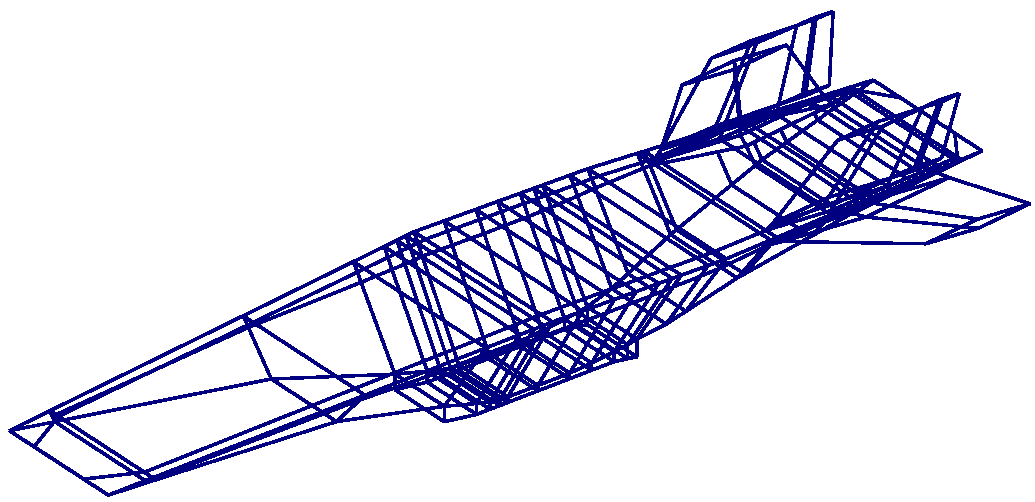
\includegraphics[width=4in]{./Images/frontispiece.pdf}}

% Default style for front pages
\frontpagestyle{1}

%% Dedication
\dedication{\topskip0pt
\pagebreak
\vspace*{\fill}
\begin{center}
  To Dad
\end{center}
\vspace*{\fill}
\pagebreak

%%% Local Variables:
%%% mode: latex
%%% TeX-master: "../main"
%%% End:
}

%% Acknowledgments
%\include{./Content/Acknowledgements}
% This command sets the width of the acknowledgments area as a fraction
% of the total width of the text area.
%\acknowledgmentswidth{0.8}

%% Preface
%\preface[2]{ %
%}

% Committee
\committee{
Assistant Professor Eric Johnsen, Chair \\
Professor David R. Dowling\\%, Mechanical Engineering, University of Michigan\\
Professor William Schultz\\%, Mechanical Engineering, University of Michigan\\
Professor Douglas L. Miller\\%, Radiology, University of Michigan
Professor J. Brian Fowlkes
}

%% Chair must be entered separately for formatting reasons.
\chair{Eric Johnsen}

%% What deliverable requirement does this fill
\deliverable{Dissertation}

% Commands to hide or show lists of figures, tables, etc.
% \hidelistoftables
% \hidelistofprograms
% \hidelistofappendices
% \hidelistoffigures
% \hidelistofabbreviations
\hidededication

%\showlistoftables
%\showlistofprograms
%\showlistofappendices
%\showlistofabbreviations
%\showlistoffigures



%% Definition of any abbreviations used.
\abbreviations{
 \acro{CEUS}{Contrast-Enhanced Ultrasound}
 \acro{CFD}{Computational Fluid Dynamics}
 \acro{DG}{Discontinuous Galerkin}
 \acro{DUS}{Diagnostic Ultrasound}
 \acro{HIFU}{High Intensity Focused Ultrasound}
 \acro{IC}{Inertial Cavitation} 
 \acro{LH}{Lung hemorrhage}
 \acro{MC}{Monte Carlo}
 \acro{PD}{Pulse Duration}
 \acro{PDF}{Probability Distribution Function}
 \acro{PFP}{Perfluoropropane}
 \acro{PRF}{Pulse Repetition Frequency}
 \acro{PRPA}{Peak Rarefaction Pressure Amplitude}
 \acro{RMI}{Richtmyer-Meshkov Instability}
 \acro{TL}{Transmission Loss}
 \acro{US}{Ultrasound}


%%% Local Variables:
%%% mode: latex
%%% TeX-master: "../main"
%%% End:

}

%% Some abstract text
\abstract{\begin{center}
  \begin{minipage}{0.8\textwidth}
    \subsection*{Abstract}
    \ac{DUS} of the lung has been shown to cause hemorrhage in a
    variety of mammals, though the underlying damage mechanism is yet
    to be determined. Motivated by this problem we model an alveolar
    tissue-air interface as a perturbed water-air interface and
    simulate its interaction with trapezoidal acoustic waves to
    investigate the underlying physics. We find that baroclinic
    vorticity is generated along the interface as a result of
    misalignment between acoustic pressure gradients and the density
    gradients across the interface. This vorticity remains continues
    to deform the interface long after all of the acoustic waves have
    passed. We postulate that this nonlinear effect is important
    because of the sharp density gradient that occurs at the water-air
    interface.

    Unlike shocks, whose interactions with fluid-fluid interfaces is
    well studied and nearly instantaneous, the acoustic waves
    considered here interact with the interface over variable, finite
    amounts of time. The effect of this interaction time is shown to
    have a significant impact on the growth of the interface
    perturbation for acoustic waves of similar amplitude and shape. We
    show that this is a result of changes in vorticity deposition that
    occur due to interface deformation that occurs during the
    interaction with the
    wave.

    Finally, We additionally perform analysis to predict the location
    of vorticity generation and growth of the interface, which we
    compare to the observed computational results.
  \end{minipage}
\end{center}
%%% Local Variables:
%%% mode: latex
%%% TeX-master: "../main"
%%% End:
}
\hideabstractpagenumber

%\usepackage{fullpage}
\usepackage{hyperref}
\usepackage{graphicx}
\usepackage{natbib}
\usepackage{pdflscape}
\usepackage{mathrsfs}
\usepackage{rotating}
\usepackage[usenames,dvipsnames]{xcolor}
\usepackage{tikz}
\usepackage{pgfgantt}
%\usepackage{typearea}
\usepackage{abstract}
\usepackage{verbatim}
\usepackage{tabularx}
\usepackage{caption}
\usepackage{subcaption}
\usepackage{embedfile}
\usepackage{import}
\usepackage[normalem]{ulem}

% My commands
\newcommand{\ganttgroupc}[5][none]{\ganttgroup[group/.append style={draw=black, fill=#1}, group incomplete/.append style={draw=black,fill=#1!50}, progress=#2]{#3}{#4}{#5}}
\newcommand{\ganttbarc}[5][none]{\ganttbar[bar/.append style={draw=black, fill=#1}, bar incomplete/.append style={draw=black,fill=#1!50}, progress=#2]{#3}{#4}{#5}}
\newcommand{\bs}[1]{\boldsymbol{#1}}
\newcommand{\del}[0]{\nabla}
\newcommand{\orderof}[1]{\ensuremath{\mathcal{O}\left(#1\right)}}
\newcommand{\abs}[1]{\ensuremath{\left|#1\right|}}
\newcommand{\norm}[1]{\ensuremath{\left\Vert#1\right\Vert}}
\newcommand{\plus}{\raisebox{.2\height}{\scalebox{.8}{+}}}

%% Declare math operators
\DeclareMathOperator{\sech}{sech}
\DeclareMathOperator{\csch}{csch}
\DeclareMathOperator{\arcsec}{arcsec}
\DeclareMathOperator{\arccot}{arcCot}
\DeclareMathOperator{\arccsc}{arcCsc}
\DeclareMathOperator{\arccosh}{arcCosh}
\DeclareMathOperator{\arcsinh}{arcsinh}
\DeclareMathOperator{\arctanh}{arctanh}
\DeclareMathOperator{\arcsech}{arcsech}
\DeclareMathOperator{\arccsch}{arcCsch}
\DeclareMathOperator{\arccoth}{arcCoth}  

% Create a snapshot of dependencies and place in .dep file
\RequirePackage{snapshot}

% Embed files
\embedfile{./content/embed_files.tex}
\embedfile{./content/abstract.tex}
\embedfile{./content/intro.tex}
\embedfile{./content/methods.tex}
\embedfile{./content/analysis.tex}
\embedfile{./content/results.tex}
\embedfile{./content/conclusions.tex}
\embedfile{./content/future.tex}
%                                                               
%
%%% Local Variables:
%%% mode: latex
%%% TeX-master: "main"
%%% End:

\embedfile{./main.tex}

% Setup latexdiff
%DIF PREAMBLE EXTENSION ADDED BY LATEXDIFF
%DIF UNDERLINE PREAMBLE %DIF PREAMBLE
\RequirePackage[normalem]{ulem} %DIF PREAMBLE
\RequirePackage{color}\definecolor{RED}{rgb}{1,0,0}\definecolor{BLUE}{rgb}{0,0,1} %DIF PREAMBLE
\providecommand{\DIFadd}[1]{{\protect\color{blue}\uwave{#1}}} %DIF PREAMBLE
\providecommand{\DIFdel}[1]{{\protect\color{red}\sout{#1}}}                      %DIF PREAMBLE
%DIF SAFE PREAMBLE %DIF PREAMBLE
\providecommand{\DIFaddbegin}{} %DIF PREAMBLE
\providecommand{\DIFaddend}{} %DIF PREAMBLE
\providecommand{\DIFdelbegin}{} %DIF PREAMBLE
\providecommand{\DIFdelend}{} %DIF PREAMBLE
%DIF FLOATSAFE PREAMBLE %DIF PREAMBLE
\providecommand{\DIFaddFL}[1]{\DIFadd{#1}} %DIF PREAMBLE
\providecommand{\DIFdelFL}[1]{\DIFdel{#1}} %DIF PREAMBLE
\providecommand{\DIFaddbeginFL}{} %DIF PREAMBLE
\providecommand{\DIFaddendFL}{} %DIF PREAMBLE
\providecommand{\DIFdelbeginFL}{} %DIF PREAMBLE
\providecommand{\DIFdelendFL}{} %DIF PREAMBLE
%DIF END PREAMBLE EXTENSION ADDED BY LATEXDIFF


%%% Local Variables:
%%% mode: latex
%%% TeX-master: t
%%% End:



%% DOCUMENT AREA

\begin{document}
\chapter*{Foreword} \label{ch:foreword}
This dissertation will present work using computation to make
advancements in two separate and distinct areas of acoustics:
ultrasound bioeffects modeling and acoustic transmission loss
uncertainty quantification in uncertain ocean environment. Hence this
document is split into two parts along these lines. A summary of
relevant background information, work performed, and conclusions in
each area will be presented separately.
%%% Local Variables:
%%% mode: latex
%%% TeX-master: t
%%% End:



%Abstract
%\begin{center}
  \begin{minipage}{0.8\textwidth}
    \subsection*{Abstract}
    \ac{DUS} of the lung has been shown to cause hemorrhage in a
    variety of mammals, though the underlying damage mechanism is yet
    to be determined. Motivated by this problem we model an alveolar
    tissue-air interface as a perturbed water-air interface and
    simulate its interaction with trapezoidal acoustic waves to
    investigate the underlying physics. We find that baroclinic
    vorticity is generated along the interface as a result of
    misalignment between acoustic pressure gradients and the density
    gradients across the interface. This vorticity remains continues
    to deform the interface long after all of the acoustic waves have
    passed. We postulate that this nonlinear effect is important
    because of the sharp density gradient that occurs at the water-air
    interface.

    Unlike shocks, whose interactions with fluid-fluid interfaces is
    well studied and nearly instantaneous, the acoustic waves
    considered here interact with the interface over variable, finite
    amounts of time. The effect of this interaction time is shown to
    have a significant impact on the growth of the interface
    perturbation for acoustic waves of similar amplitude and shape. We
    show that this is a result of changes in vorticity deposition that
    occur due to interface deformation that occurs during the
    interaction with the
    wave.

    Finally, We additionally perform analysis to predict the location
    of vorticity generation and growth of the interface, which we
    compare to the observed computational results.
  \end{minipage}
\end{center}
%%% Local Variables:
%%% mode: latex
%%% TeX-master: "../main"
%%% End:

\chapter{Introduction} \label{ch:Introduction}
The purpose of this introduction is to set the stage for the proposed
dissertation research. The problems we approach in this work are all
problems of interest, current to the field of Acoustics. Broadly,
acoustics is the study of sound. In practice, this study is not
limited to just the kinds of sound that can be heard by humans, but
rather any molecular scale vibrations traveling throughout a media. As
sounds both natural and man-made are ubiquitous, it is a topic that
has intrigued man for quite some time and attracted much attention and
study. As such, we have gained not only an understand the physical
nature of sound, but have also learned to harness it as a
tool. Because sound waves travel reflect, transmit, and scatter in a
mathematically describable way, they are ideally suited for gathering
information in certain situations. Because they carry mechanical
energy that can be focused, concentrated, and in some instances
converted into other types of energy, such as heat, they can also be a
powerful tool for physically altering an environment. In some
applications of interest, attempts to use acoustics to gather
information, can unintentionally lead to physical modification of the
system, such is the case when \ac{DUS} for medical imaging leads to
unintended biological effects, or ultrasound bioeffects as we will
refer to them from here on out.

Many problems of contemporary acoustic interest present challenges
that make them difficult to investigate completely through direct
experimentation. Some problems, such as certain ultrasound bioeffects,
often involve physical processes that occur over such small length and
time scales that they cannot be directly observed. When these
phenomena are replicated in simplified lab experiments, as they
frequently are, physical quantities of interest, like stress, are not
always readily measurable. Other problems may call for experiments
that are prohibitively costly and time-intensive, as is often the case
in underwater and ocean acoustics experiments which can require long
cruises with extensive personnel and equipment. Furthermore, in
complex acoustic environments like the ocean or human body, we rarely
have sufficient information to precisely and accurately describe the
system of interest without a high degree of uncertainty. In instances
such as these, where direct experimentation is infeasible or unable to
provide the desired information, carefully designed numerical
experiments can be useful for providing insight into the
problem at hand. 

The unifying theme of the work presented here is the use of
computation to approach modern problems in acoustics. The two main
areas of research considered are \acf{US} bioeffects and underwater
acoustic uncertainty. In the first part of this work, we investigate
two problems related to biological effects of medical
\ac{US}. Specifically, we simulate physics associated with \ac{CEUS}
and \ac{DUS} of the lung, which have both been shown to be capable of
causing hemorrhage in mammals, in order to investigate the damage
mechanism behind each. In the second part of this work we develop and
test area statistics, a computationally efficient method for
estimating the \ac{PDF} of acoustic \ac{TL} in uncertain ocean
environments, which is useful in naval applications. As these areas
are appreciably different, we will refer the reader to later portions
of this document and to the authors relevant submitted and published
works for more detailed introduction and background on each problem.

% %\subsection{\ac{US} background}
% Diagnostic \ac{US} has proven to be among the safest and most powerful
% medical imaging tools currently available and its use has become
% ubiquitous throughout modern medicine. The basic physical principle
% underlying this technology the scattering of sound at material
% interfaces. In practice, high-frequency, typically MHz range, acoustic
% waves and pulses are created at the surface of the body using a
% piezoelectric \ac{US} transducer. These vibrations propagate via an
% acoustic coupling medium from the transducer into the tissue and
% scatter whenever they encounter a change in the material properties of
% the medium. More simply, some of the sound echoes whenever it moves
% from one tissue to another, or hits a cavity in the body. These echoes
% are then picked up by a receiver and recorded. The strength and timing
% of these echoes allow for real-time imaging of the scattering surface.

% While clinical \ac{US} is generally incredibly safe there are
% specific instances during which \ac{US} can interact with tissue in
% such a way that it physically alters tissue. These effects to the body
% are referred to as \ac{US} bioeffects. While the entire field of
% therapeutic \ac{US} is based around intentionally causing
% bioeffects in a way that is beneficial to the patient, diagnostic
% \ac{US} is a different story. Bioeffects that occur during
% diagnostic \ac{US} typically take the form of unintended tissue
% damage or cell death. Depending on the type of physical damage
% mechanism responsible, these bioeffects are classified into two
% groups, thermal and non-thermal. The first group, thermal bioeffects
% are characterized by deposition of acoustic energy into tissue as
% heat. At the cellular and molecular scales, this can lead to the
% release of highly reactive free radicals, protein denaturation, and
% ultimately tissue damage and death. Little else will be said about
% thermal bioeffects, as the the bioeffects problems of interest to this
% work fall into the non-thermal category. The bulk of known non-thermal
% bioeffects are attributed to acoustically-induced cavitation.  

% Acoustic cavitation is the phenomenon by which gas nano and
% microbubbles, called cavitation nuclei, are cyclically grown by low
% pressures within the \ac{US} field and then collapsed high
% pressures within the field. When the bubble dynamics during collapse
% are dominated by the inertia of the surrounding fluid, it is called
% \ac{IC}. \ac{IC} is typically violent and results in the
% bubble collapsing to a fraction of its original size. There are
% several possible damage mechanisms associated with \ac{IC} that may be
% responsible for observed \ac{US} bioeffects. Upon collapse, the
% pressure and temperature within the bubbles spike, often reaching
% billions of pascals and thousands of Kelvin respectively. Due to the
% pressure difference between the vapor/gas mixture within the bubble at
% collapse and the surrounding media, the collapsed bubble can emit a
% powerful shock wave which can be damaging to the bubbles
% surroundings. When cavitation is triggered near a rigid surface, the
% bubble can collapse in a radially asymmetric fashion causing a high
% speed ``re-entrant'' jet of liquid to impinge upon the surface,
% effectively striking the surface with a liquid hammer \hl{CITE}. If
% cavitation occurs at an appropriate distance from a non-rigid surface,
% such as soft tissue boundaries and blood vessel walls, the jet can
% impinge away from the surface, potentially invaginating the surface
% \citep{Brujan2011}. \ac{CEUS}, which uses
% contrast-agent microbubbles injected into patients bloodstream to act
% as additional scattering surfaces. These microbubbles act as
% cavitation nuclei and have been associated with a variety of different
% forms of cellular death and damage.

% This proposal presents past work in which we simulate ultrasonically
% induced cavitation of contrast agent microbubbles in soft tissue
% \citep{Patterson2012} (See Chapter \ref{ch:usbe_bubble}).  We simulate
% experimentally measured \ac{US} waves obtained by \cite{Miller2008b}
% perturbing microbubbles in a Voigt viscoelastic soft tissue
% \cite[]{Yang2005}. The calculated cavitation dynamics and theoretical
% inertial cavitation thresholds \citep{Flynn1982,Apfel1982} are
% compared with bioeffects thresholds associated with each \ac{US}
% pulse, as defined by the observation of kidney hemorrhage in rats
% after exposure to CEUS by \cite{Miller2008b}. While the results were
% generally dependent on US, gas, and tissue properties, it was found
% that the inertial cavitation thresholds were lower than observed
% bioeffects thresholds.

% Another non-thermal \ac{US} bioeffect of interest is \ac{DUS}-induced
% \ac{LH}, which is the only known bioeffect of non-contrast \ac{DUS}
% known to occur in mammals. Despite the fact that this phenomenon was
% first observed in mice over twenty years ago \citep{Child1990}, the
% underlying physical damage mechanisms remain unknown. Research has
% shown that thermal damage mechanisms are unlikely as \ac{DUS}-induced
% lung lesions do not appear similar to those induced by heat
% \citep{Zachary2006}. Furthermore, cavitation mechanisms do not appear
% to be responsible, as the severity of \ac{DUS}-induced \ac{LH} in mice
% increased under raised hydrostatic pressure \citep{OBrien2000} and was
% unaffected by the introduction of \ac{US} contrast agents into
% subjects. Both of these results are inconsistent with what is expected
% of \ac{IC}-induced bioeffects. Works by \cite{Tjan2007,Tjan2008} model
% the evolution of an inviscid, free surface subjected to a Gaussian
% velocity potential and find that this can lead to the ejection of
% liquid droplets. They go on to say that \ac{DUS} of the lung may
% similarly lead to the ejected of droplets capable of puncturing the
% air-filled sacs within the lung. We propose another possible damage
% mechanism, that \ac{DUS} pulses torque tissue-air interfaces around
% alveoli, fragile air-sacs within the lungs. This deposits vorticity, a
% measure of local fluid rotation, in the surrounding fluid which drives
% deformation and ultimately hemorrhage of the thin alveolar walls.

% The concept of vorticity driven interface deformation has been
% extensively studied within the context of the \ac{RM}, which occurs
% when a traveling pressure wave, typically a shock, encounters a
% perturbed interface between fluids of different density. Note that the
% \ac{RM} is not a true instability, as the interface does not exhibit
% exponential growth. When this occurs vorticity is generated along the
% interface.

% As can be seen from the
% vorticity generation equation,
% \begin{align} \label{eq:vorticity}
% \frac{\partial \vec{\omega}}{\partial t}+\left(\vec{u}\cdot\nabla\right)\vec{\omega} = 
% \left(\vec{\omega\cdot\nabla}\right)\vec{u} - \vec{\omega}\left(\nabla\cdot\vec{u}\right)%
% +\frac{\nabla\rho\times\nabla p}{\rho^2} + \nabla\times\left(\frac{\nabla\cdot\tau}{\rho}\right)%
% +\nabla\times\left(\frac{\vec{B}}{\rho}\right)%
% \end{align}


% Computations of acoustic transmission loss are of practical interest in a variety of naval applications.






%%% Local Variables:
%%% mode: latex
%%% TeX-master: "../../main"
%%% End:

\acresetall

% % US Bioeffects
\part{Ultrasound bioeffects} \label{part:ultrasound_bioeffects}
\chapter{Introduction} \label{ch:usbe_intro}%
The purpose of this chapter is two fold. First, we aim to provide a
general physical context for the work presented in this part of the
thesis proposal. Second, we will provide a brief overview of the work
to be presented and its significance. For a more detailed overview of
the relevant literature, the reader is referred to later parts of this
document, and to this authors published works.

\section{Physical context} \label{sec:usbe_intro_physical_context}%
Diagnostic \ac{US} has proven to be among the safest and most powerful
medical imaging tools currently available. Its use has become
ubiquitous throughout modern medicine. The basic physical principle
underlying this technology is the scattering of sound at material
interfaces. In practice, high-frequency, typically MHz range, acoustic
waves and pulses are created at the surface of the body using a
piezoelectric \ac{US} transducer. These vibrations propagate via an
acoustic coupling medium from the transducer into the tissue and
scatter at changes in the material properties of the medium. More
simply, some of the sound echoes whenever it moves from one tissue to
another, or hits a cavity in the body. These echoes are then picked up
by a receiver and recorded. This echo signal is processed to obtain
real-time images of the scattering surface.

While clinical \ac{US} is typically safe there are specific instances
during which \ac{US} can interact with tissue in such a way that the
tissue is physically altered. These effects to the body are referred
to as \ac{US} bioeffects. Understanding these \ac{US}-tissue
interactions is important for the development of safe, effective
\ac{US} techniques \citep{Dalecki2004}. While the entire field of
therapeutic \ac{US} is focused on intentionally causing bioeffects in
a way that is beneficial to the patient, diagnostic \ac{US} is a
different story. Bioeffects that occur during diagnostic \ac{US}
typically take the form of unintended hemorrhage, tissue damage, or
cell death. Depending on the physical damage mechanism responsible,
these bioeffects are broadly classified into two groups, thermal and
non-thermal \citep{OBrien2007}. The first group, thermal bioeffects
are characterized by deposition of acoustic energy into tissue as
heat. At the cellular and molecular scales, this can lead to the
release of highly reactive free radicals, protein denaturation, and
ultimately tissue damage and death. Little else will be said about
thermal bioeffects, as the bioeffects problems of interest to this
work are a result of non-thermal mechanisms. 

The bulk of known non-thermal bioeffects are attributed to
acoustically-induced cavitation. Acoustic cavitation is the phenomenon
by which gas nano and microbubbles, called cavitation nuclei, are
cyclically grown by low pressures within the \ac{US} field and then
collapsed high pressures within the field. Cavitation can be divided
into two categories, stable cavitation, also called gas body
activation, and \ac{IC}, formerly referred to as transient
cavitation. Stable cavitation typically occurs for low \ac{US}
intensity an is characterized by bubbles periodically oscillating
around an equilibrium radius for multiple acoustic cycles. \ac{IC}
typically occurs for higher ultrasound intensities. During \ac{IC} the
bubble dynamics during collapse are dominated by the inertia of the
surrounding fluid. The bubble collapses violently to a tiny fraction
of its original size and then explosively rebounds back. There are
variety of physical phenomena associated with \ac{IC} that may be
responsible for observed \ac{US} bioeffects. Upon collapse, the
pressure and temperature within the bubbles spike, often reaching
billions of pascals and thousands of Kelvin respectively. Due to the
pressure difference between the vapor/gas mixture within the bubble at
collapse and the surrounding media, the collapsed bubble can emit a
powerful shock wave. When cavitation is triggered near a rigid
surface, the bubble can collapse in a radially asymmetric fashion
causing a high speed ``re-entrant'' jet of liquid to impinge upon the
surface, effectively striking the surface with a liquid hammer. If
cavitation occurs at an appropriate distance from a non-rigid surface,
such as soft tissue boundaries and blood vessel walls, the jet can
impinge away from the surface, potentially invaginating the surface
\citep{Brujan2011}. One type of \ac{DUS} for which cavitation is of
particular concern is \ac{CEUS}, which uses contrast-agent
microbubbles injected into patients bloodstream to act as additional
scattering surfaces. These microbubbles can also serve as cavitation
nuclei and have been associated with a variety of \ac{US} bioeffects. 

Another non-thermal \ac{US} bioeffect of interest is \ac{DUS}-induced
\ac{LH}, which is the only known bioeffect of non-contrast \ac{DUS}
known to occur in mammals. Despite the fact that this phenomenon was
first observed in mice over twenty years ago \citep{Child1990}, the
underlying physical damage mechanisms remain unknown. Research has
shown that thermal damage mechanisms are unlikely as \ac{DUS}-induced
lung lesions do not appear similar to those induced by heat
\citep{Zachary2006}. Furthermore, cavitation mechanisms do not appear
to be responsible, as the severity of \ac{DUS}-induced \ac{LH} in mice
increased under raised hydrostatic pressure \citep{OBrien2000} and was
unaffected by the introduction of \ac{US} contrast agents into
subjects. Both of these results are inconsistent with what is expected
of \ac{IC}-induced bioeffects. Works by \cite{Tjan2007,Tjan2008} model
the evolution of an inviscid, free surface subjected to a Gaussian
velocity potential and find that this can lead to the ejection of
liquid droplets. They go on to say that \ac{DUS} of the lung may
similarly lead to the ejected of droplets capable of puncturing the
air-filled sacs within the lung. This problem is central to the our
present and future work, and makes up the bulk of this proposal. As
such, a far more in-depth literature review will be provided in
Chapter \ref{ch:usbe_lung}.

\section{An overview of our work studying \ac{US}
  bioeffects} \label{sec:usbe_intro_overview}%
For the proposed dissertation, we will discuss our work studying two
ultrasound bioeffects problems. 

First, in Chapter \ref{ch:usbe_bubble} we present past work in which
we simulate ultrasonically induced cavitation of contrast agent
microbubbles in soft tissue \citep{Patterson2012}. We use
experimentally measured $1.5-7.5$ MHz \ac{US} waves, previously used
by \cite{Miller2008b} to determine kidney capillary hemorrhage
threshold amplitudes in rats, as input to the simulation. The
calculated cavitation dynamics and theoretical inertial cavitation
thresholds \citep{Flynn1982,Apfel1982} are compared with known
thresholds for kidney hemorrhage to investigate their dependence on
US, gas, and tissue properties. At the time of its publication, this
work was unique in its combination of experimental results and
numerical modeling to approach this problem.

Second, in Chapter \ref{ch:usbe_lung} we present current work
investigating a previously unconsidered potential mechanism for
\ac{DUS}-induced \ac{LH}. We develop a model of \ac{DUS}-alveolus
interaction as an acoustically accelerated interface between two
compressible fluids and perform numerical simulations to show that
acoustically generated baroclinic torque at tissue-air interfaces
within the lungs may be capable of deforming the fragile alveolar
walls within the lungs, possibly to the point of hemorrhage. We
generalize our discussion to acoustically-accelerated, perturbed,
liquid-gas interfaces. Finally we propose future work to be completed
for this dissertation.
%%% Local Variables:
%%% mode: latex
%%% TeX-master: "../../prelim"
%%% End:


% % US Bioeffects: 2012 Jasa Paper
\chapter{\textit{Past work:} Theoretical microbubble Dynamics at capillary breaching thresholds}   \label{ch:usbe_bubble}%
%\section{Abstract}
  In order to predict bioeffects in contrast-enhanced diagnostic and
  therapeutic ultrasound procedures, the dynamics of cavitation
  microbubbles in viscoelastic media must be determined.  For this
  theoretical study, measured 1.5-7.5 MHz pulse pressure waveforms,
  which were used in experimental determinations of capillary
  breaching thresholds for contrast-enhanced diagnostic ultrasound in
  rat kidney, were used to calculate cavitation nucleated from
  contrast agent microbubbles.  A numerical model for cavitation in
  tissue was developed based on the Keller-Miksis equation (a
  compressible extension of the Rayleigh-Plesset equation for
  spherical bubble dynamics), with a Kelvin-Voigt constitutive relation. From
  this model, the bubble dynamics corresponding to the experimentally
  obtained capillary breaching thresholds were determined. Values of
  the maximum radius and temperature corresponding to previously
  determined bioeffect thresholds were computed for a range of
  ultrasound pulses and bubble sizes for comparison to inertial
  cavitation threshold criteria.  The results were dependent on
  frequency, the gas contents, and the tissue elastic properties.  The
  bioeffects thresholds were above previously determined inertial
  cavitation thresholds, even for the tissue models, suggesting the
  possibility of a more complex dosimetry for capillary injury in
  tissue.


%%% Local Variables:
%%% mode: latex
%%% TeX-master: t
%%% End:

In this chapter we present work in which experimentally-measured
\ac{US} pulses are used to simulate \ac{US} contrast agent microbubble
dynamics. The pulses were previously used in experiments to determine
capillary breaching thresholds in rat kidneys \citep{Miller2008b}. We
compare the calculated bubble dynamics to the
experimentally-determined bioeffects thresholds to investigate the use
of theoretical \ac{IC} thresholds as a predictor for bioeffects. This
work was published in the Journal of the Acoustical Society of America
\citep{Patterson2012, Patterson2012a}. Here we present the abstract, key figures, and
conclusions of the published work.
%
\section{Abstract}
  In order to predict bioeffects in contrast-enhanced diagnostic and
  therapeutic ultrasound procedures, the dynamics of cavitation
  microbubbles in viscoelastic media must be determined.  For this
  theoretical study, measured 1.5-7.5 MHz pulse pressure waveforms,
  which were used in experimental determinations of capillary
  breaching thresholds for contrast-enhanced diagnostic ultrasound in
  rat kidney, were used to calculate cavitation nucleated from
  contrast agent microbubbles.  A numerical model for cavitation in
  tissue was developed based on the Keller-Miksis equation (a
  compressible extension of the Rayleigh-Plesset equation for
  spherical bubble dynamics), with a Kelvin-Voigt constitutive relation. From
  this model, the bubble dynamics corresponding to the experimentally
  obtained capillary breaching thresholds were determined. Values of
  the maximum radius and temperature corresponding to previously
  determined bioeffect thresholds were computed for a range of
  ultrasound pulses and bubble sizes for comparison to inertial
  cavitation threshold criteria.  The results were dependent on
  frequency, the gas contents, and the tissue elastic properties.  The
  bioeffects thresholds were above previously determined inertial
  cavitation thresholds, even for the tissue models, suggesting the
  possibility of a more complex dosimetry for capillary injury in
  tissue.


%%% Local Variables:
%%% mode: latex
%%% TeX-master: t
%%% End:


\section{Key figures}
\label{sec:usbe_bubble_key_figures}
%\subsection{Bubble Response}
In this section we present key figures from \cite{Patterson2012a}. The
results presented are based on simulations of microbubbles in a Voigt
viscoelastic medium as modeled by \cite{Yang2005}. Experimentally
determined input pressure waveforms and the associated bioeffects are
based on the work performed in \cite{Miller2008b}.

To illustrate typical bubble responses, Figures
\ref{fig:sample_bubble_linear} and \ref{fig:sample_bubble_nonlinear}
show sample experimental input pressure waveforms from
\citep{Miller2008b} and the calculated bubble radius histories
corresponding to each. Both simulations are for the case of the wave
impinging upon an initially $R_0=1 \mu$m radius microbubble in Voigt
viscoelastic media with shear moduli, $G=5$ kPa, $100$ kPa, and $1$
MPa as indicated. Figure \ref{fig:sample_bubble_linear} represents an
essentially linear case with \ac{US} center frequency 1.5 MHz and 0.35
MPa \ac{PRPA}, in which no bioeffects were observed. Figure
\ref{fig:sample_bubble_nonlinear} represents a highly nonlinear case
with 7.5 MHz and 6.0 MPa \ac{PRPA}. In bioeffects, in the form of
bleeding on the surface of the rat kidney, were observed
\cite{Miller2008b}.
\begin{figure}%[h!]
  \centering
  \includegraphics[width=0.66\textwidth]{./figs/bubble_figs/rt_linear}
  \caption[Bubble radius history and input-pressure for an essentially linear case]{History of the bubble radius (top) and input-pressure
    waveform (bottom) for an essentially linear case (frequency: 1.5 MHz; \ac{PRPA}: 0.35 MPa). No bioeffects are observed
    here. $R_0=1$ $\mu$m; solid: $G=5$ kPa; dashed: $G=100$ kPa; dotted: $G=1$ MPa.}
  \label{fig:sample_bubble_linear}
\end{figure}
%
\begin{figure}%[h!]
  \centering \includegraphics[width=0.66\textwidth]{./figs/bubble_figs/rt_nonlinear}
  \caption[Bubble radius history and input-pressure for a nonlinear case]{History of the bubble radius (top) and input-pressure
    waveform (bottom) for a highly nonlinear case (frequency: 
    7.5 MHz; peak negative pressure: 6.0 MPa). Bioeffects are observed
    here. $R_0=1$ $\mu$m; solid: $G=5$ kPa; dashed: $G=100$ kPa; dotted: $G=1$ MPa.}
  \label{fig:sample_bubble_nonlinear}
\end{figure}

To study the dependence of the bubble dynamics on the gas content, we
compare results obtained for bubbles containing \ac{PFP} and air.
Figure \ref{fig:gascontents} shows sample bubble radii histories for
each gas and the corresponding input pressure wave. Additionally, we
plot of the maximum temperature for \ac{PFP} (circles) and air
(squares), calculated based on isentropic relationships, for bubbles
with initial radii $R_0=0.1-2$ $\mu$m exposed to ultrasound
frequencies 1.5 - 7.5 MHz and \ac{PRPA} 0.35 - 6 MPa.
\begin{figure*}%[h!]
  \includegraphics[width=0.47\textwidth]{./figs/bubble_figs/pfpair}% }
  \includegraphics[width=0.47\textwidth]{./figs/bubble_figs/tmaxpfpair}% }
  \caption[Dependence of the bubble dynamics on the gas contents]{ Dependence of the bubble dynamics on the gas contents ($G=100$ kPa). (Left) History of the bubble radius for \ac{PFP} (solid) 
    and air (dashed). (Right) Maximum temperature for \ac{PFP} (circles) and air (squares). $R_0=0.1-2$ $\mu$m; frequency: 1.5 - 7.5 MHz. }
  \label{fig:gascontents}
\end{figure*}

To illustrate the dependence of the bubble response on the pulse
frequency Figure \ref{fig:freq} shows the maximum dimensionless and
dimensional radius for all initial bubble sizes and amplitudes vs
frequency. The square symbols denote cases in which bioeffects were
observed in the experiments, while the circular symbols represent no
bioeffects. The initial bubble sizes are not discriminated here for
simplicity. With the exception of a few outliers, a clear separation
between cases for which bioeffects did and did not occur is observed;
in other words, the bioeffect threshold has a strong dependence on the
frequency. The trend appears to be approximately linear with
frequency. Large growth may be achieved with no evident bioeffects,
especially at high frequencies. The quantity $R_{max}$ is a measure of
cavitation collapse since it is related to the available energy of the
bubble. Thus, the present results indicate that cavitation collapse is
expected to play an important role regarding bioeffects, although the
precise mechanism cannot be inferred. Again, the existing criteria for
inertial cavitation thresholds are frequency-independent and do not
correlate well with the bioeffects threshold, which clearly shows a
strong dependence on frequency.
\begin{figure*}%[h!]
  \includegraphics[width=0.47\textwidth]{./figs/bubble_figs/rstarmax_f}  
  \includegraphics[width=0.47\textwidth]{./figs/bubble_figs/rmax_f}      
  \caption[Dependence of the bubble dynamics on the ultrasound frequency]{ Dependence of the bubble dynamics on the frequency for
    $G=100$ kPa. $R_0=0.1-2$ $\mu$m; empty circles: no bioeffects; squares:
    bioeffects. (Left) Dimensionless (Left) and dimensional (Right) maximum bubble radius.}
  \label{fig:freq}
\end{figure*}

To explore the effect of the elasticity on the results and the
correlation to bioeffects, Figure \ref{fig:freq_tissue} shows the
maximum dimensionless radius for all initial bubble sizes and
amplitudes vs frequency for $G=5$ kPa and $G=1$ MPa. Although
seemingly high, the latter elasticity is chosen to match the work of
\begin{figure*}%[h!]
  \includegraphics[width=0.47\textwidth]{./figs/bubble_figs/rstarmax_f_ca=20}
  \includegraphics[width=0.47\textwidth]{./figs/bubble_figs/rstarmax_f_ca=0,1}    
  \caption[Dependence of the dimensionless maximum bubble radius on
    the ultrasound frequency]{ Dependence of the dimensionless maximum bubble radius on
    the frequency for $G=5$ kPa (Left) and $G=1$ MPa (Right). $R_0=0.1-2$ $\mu$m; empty circles: no bioeffects; squares:
    bioeffects. }
  \label{fig:freq_tissue}
\end{figure*}

% \begin{figure*}[h!]
%   \subfigure[$G=5$ kPa.]{
%     \includegraphics[width=0.47\textwidth]{./figs/bubble_figs/rstarmax_f_ca=20}
%   }
%   \subfigure[$G=1$ MPa.]{
%     \includegraphics[width=0.47\textwidth]{./figs/bubble_figs/rstarmax_f_ca=0,1}    
%   }
%    \caption{ Dependence of the dimensionless maximum bubble radius on
%      the frequency. $R_0=0.1-2$ $\mu$m; empty circles: no bioeffects; squares:
%      bioeffects.}
%   \label{fig:freq_tissue}
% \end{figure*}
\clearpage
\pagebreak
\section{Conclusions}
\label{sec:conclusions}

In the present work, a numerical model is used
to investigate experimentally observed bioeffects as a result of
contrast-enhanced ultrasound. This work is unique in its 
combination of experimental results and numerical modeling.
For the experimentally generated input
pressure waveforms, it is known which of these triggered bioeffects,
and from the numerical model we obtained calculated values for
the dimensionless maximum radius and dimensional maximum temperature for each of these cases.  By comparing the
results of this study to previously established inertial cavitation
thresholds used by \cite{Apfel1991} and \cite{Yang2005},
$T_{max}=5000$ K and $R_{max}=2$, it would appear that the inertial
cavitation threshold does not play a role in determining the bioeffects
threshold.  However, it is unlikely that the inertial cavitation
threshold is irrelevant. Instead, it is far more probable that these
thresholds are not defined appropriately for cavitation in a
viscoelastic medium, such as soft tissue. This work suggests the need for
further experimental and numerical studies of cavitation in viscoelastic media.

The present work shows a strong correlation between cavitation dynamics and bioeffects
when considering the pulse frequency.
From the plot of maximum
dimensionless radius vs. frequency, there is a clear separation
between when bioeffects do and do not occur, and based on these
results it appears that the frequency of the input pressure waveforms
is of key importance to the definition of a bioeffect threshold, and
likely the inertial cavitation threshold as well. 

The present work shows that the elasticity of tissue significantly
affects the bubble dynamics. This finding is perhaps not completely
unexpected given that bubble dynamics are known to strongly depend
on viscoelastic properties and model. The present study shows the need
for more accurate measurements of material properties and for
determining appropriate constitutive models for soft tissue,
particularly at high strain rates. Finally, although the present work
suggests that inertial cavitation collapse plays an important role with respect
to bioeffects, it does not shed light on the exact mechanism,
\emph{e.g.}, shock emission upon collapse, growth beyond a given size,
high temperatures generating free radicals, re-entrant jets in
non-spherical collapse, etc.  In future work we plan on investigating 
this injury mechanism by conducting direct simulations of
the full equations of motion for bubble dynamics in a viscoelastic medium.


%%% Local Variables:
%%% mode: latex
%%% TeX-master: "../../prelim"
%%% End:

% 
\begin{figure}
  \centering \includegraphics[width=0.66\textwidth]{./figs/bubble_figs/rt_linear}
  \caption{History of the bubble radius (top) and input-pressure
    waveform (bottom) for an essentially linear case (frequency: 1.5 MHz; peak y
    negative pressure: 0.35 MPa). No bioeffects are observed
    here. $R_0=1$ $\mu$m; solid: $G=5$ kPa; dashed: $G=100$ kPa; dotted: $G=1$ MPa.}
  \label{figure:sample_bubble_linear}
\end{figure}

\begin{figure}
  \centering 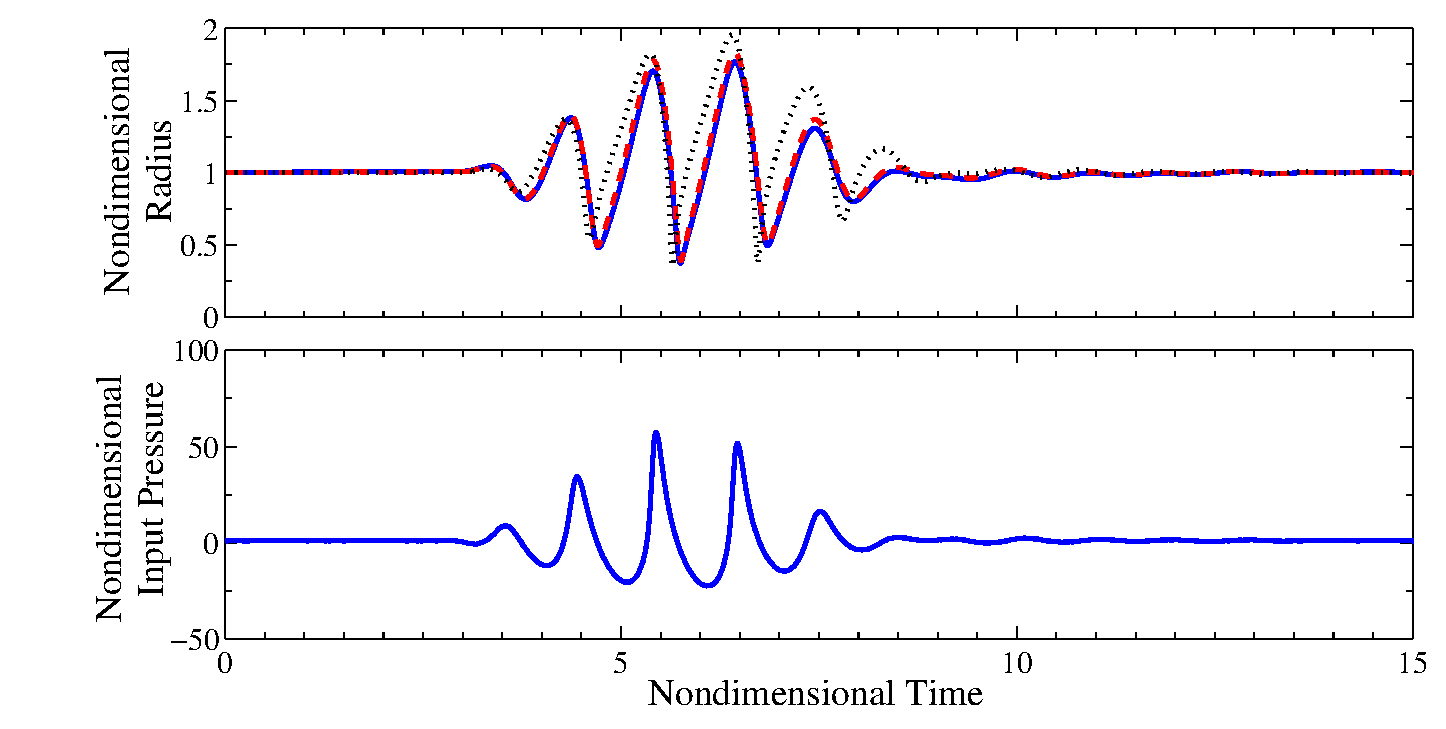
\includegraphics[width=0.66\textwidth]{./figs/bubble_figs/rt_intermediate}%
  \caption{History of the bubble radius (top) and input-pressure
    waveform (bottom) for a moderately nonlinear case (frequency: 3.5 MHz; peak 
    negative pressure: 2.4 MPa). Bioeffects are
    observed here. $R_0=1$ $\mu$m; solid: $G=5$ kPa; dashed: $G=100$ kPa;
    dotted: $G=1$ MPa.}
  \label{figure:sample_bubble_intermediate}
\end{figure}

\begin{figure}
  \centering \includegraphics[width=0.66\textwidth]{./figs/bubble_figs/rt_nonlinear}
  \caption{History of the bubble radius (top) and input-pressure
    waveform (bottom) for a highly nonlinear case (frequency: 
    7.5 MHz; peak negative pressure: 6.0 MPa). Bioeffects are observed
    here. $R_0=1$ $\mu$m; solid: $G=5$ kPa; dashed: $G=100$ kPa; dotted: $G=1$ MPa.}
  \label{figure:sample_bubble_nonlinear}
\end{figure}

In the results of the following sections, the maximum dimensionless radius,
$R_{max}$, and dimensional bubble temperature at collapse, $T_{max}$, obtained
using the ideal gas law, are determined by recording their largest
value over the simulation. These quantities are compared to the
inertial cavitation thresholds used by \cite{Apfel1991} and
\cite{Yang2005}: $R_{max}=2$ and $T_{max}=5000$ K. The dependence
of the bubble dynamics on the pulse amplitude, initial
bubble size (\emph{i.e.}, UCA size distribution), 
pulse frequency, and tissue properties are considered
individually. 



\subsection{Dependence on the Pulse Amplitude}

Given the strong dependence of the MI on the rarefactional pressure
amplitude, the influence of the pulse amplitude on the bubble dynamics
is first evaluated. Fig.~\ref{figure:amplitude} shows the dimensionless
maximum radius as a function of rarefactional pressure
amplitude. Initial bubble radii ranging between 0.1--2.0 $\mu$m are
shown, as well as different frequencies. The open symbols denote
cases where bioeffects did not occur, while the filled symbols denote
the occurrence of bioeffects.

\begin{figure}[t]
  \includegraphics[width=\columnwidth]{./figs/bubble_figs/rstarmax_pm}
  \caption{(color online) Dependence of the dimensionless maximum bubble radius on
    the peak negative pressure for $G=100$ kPa.  Empty symbols: no
    bioeffects; filled symbols: bioeffects. Pentagrams: 0.1 $\mu$m; circles:
    0.5 $\mu$m; squares: 1 $\mu$m; diamonds: 2 $\mu$m; frequency: 1.5 - 7.5 MHz. }
  \label{figure:amplitude}
\end{figure}

The results show that the bubble dynamics, through the maximum radius,
scale with the pulse amplitude. Although the results do not collapse fully
onto a line, a general trend is discernible. At low amplitude, the increase in
the maximum radius is approximately linear; beyond some amplitude, the bubble undergoes
nonlinear oscillations, thus explaining the different depenced and larger spread. 
These results are consistent with the plots shown in 
Figs.~\ref{figure:sample_bubble_linear}-\ref{figure:sample_bubble_nonlinear}.
Over a broad range of amplitudes, the
occurrence of bioeffects has little correlation with pulse amplitude
alone: at a given amplitude, bioeffects may be observed or not,
depending on the bubble size and pulse frequency.  Only at very large
pressure amplitudes (PRPA $>$ 4.20 MPa) are bioeffects systematically observed regardless of the
bubble size and pulse frequency. This behavior is not surprising, since at
these amplitudes the bubble response is expected to be highly
nonlinear. Conversely, at low amplitudes (PRPA $<$ 0.97 MPa), the oscillations are 
linear and no bioeffects are observed, regardless of
bubble size and pulse frequency. In this latter case, most bubbles
whose $R_{max}/R_o$ is below two do not exhibit bioeffects; however,
this behavior depends on the value of elasticity, as shown in \S
\ref{section:tissue_properties}.  Although not shown here for conciseness,
similar results are obtained for peak positive pressure.


Similarly, the criterion $T_{max} > 5000$ K is not achieved with perfluoropropane.
As shown in Fig.~\ref{figure:gascontents}, the observed temperatures for
PFP are far below this value, though the results for air approach it. This
result is expected since the criterion was determined for air, which
has a larger specific heats ratio ($\gamma_{air}=1.4$) than
PFP ($\gamma= 1.13$). The specific heats ratio appears in
the internal gas pressure term in Eq.~\ref{eq:bubble_pressure}; its
effect on the bubble dynamics is minor if the minimum radius is not
very small, as in Fig.~\ref{figure:gascontents}. Still, since the
adiabatic relationships for an ideal gas are used, the temperature is
significantly affected by the different specific heats ratio. Hence,
even though the bubble dynamics are not strongly affected by the
specific heats ratio, the maximum temperature is.

\begin{figure*}[t]
  \begin{subfigure}[b]{0.47\textwidth}
  \includegraphics[width=\textwidth]{./figs/bubble_figs/pfpair}
  \caption{History of the bubble radius for PFP (solid) and air
    (dashed). $R_0=1$ $\mu$m; frequency: 3.5 MHz; peak negative
    pressure: 3.3 MPa}
\end{subfigure}
  \begin{subfigure}[b]{0.47\textwidth}
    \includegraphics[width=\textwidth]{./figs/bubble_figs/tmaxpfpair} 
    \caption{Maximum temperature for PFP (circles) and air (squares). $R_0=0.1-2$ $\mu$m; frequency: 1.5 - 7.5 MHz.}
  \end{subfigure}
  \caption{(color online) Dependence of the bubble dynamics on the gas contents ($G=100$ kPa).}
  \label{figure:gascontents}
\end{figure*}

% \begin{figure*}[t]
%   \subfigure[History of the bubble radius for PFP (solid) 
%     and air (dashed). $R_0=1$ $\mu$m; frequency: 3.5 MHz; peak negative pressure: 3.3 MPa]{
%   \includegraphics[width=0.47\textwidth]{./figs/bubble_figs/pfpair} }
%   \subfigure[Maximum temperature for PFP (circles) and air (squares). $R_0=0.1-2$ $\mu$m; frequency: 1.5 - 7.5 MHz. ]{
%   \includegraphics[width=0.47\textwidth]{./figs/bubble_figs/tmaxpfpair} }
%   \caption{(color online) Dependence of the bubble dynamics on the gas contents
%   ($G=100$ kPa).}
%   \label{figure:gascontents}
% \end{figure*}






\subsection{Dependence on the Initial (Equilibrium) Bubble Radius}

In the experiment, the size distribution of the UCAs is not known
exactly. It is desirable to know whether the observed bioeffects are
caused by all bubbles responding to the ultrasound, or whether a
specific size is more likely to be responsible at the bioeffects
threshold. To answer this question, for each experimental frequency,
bubbles of different radii ranging from 0.1--2 $\mu$m are subjected to
the pressure waveform corresponding to the bioeffects threshold
amplitude. It should be noted that varying the equilibrium radius
changes the non-dimensional parameters. Fig.~\ref{figure:size} shows the maximum dimensionless
radius, for both water (zero elasticity) and tissue (finite
elasticity, $G=100$ kPa), for the amplitude at which bioeffects are
first observed at a given frequency.

\begin{figure}[t]
    \includegraphics[width=\columnwidth]{./figs/bubble_figs/rstarmax_r0}
    \caption{(color online) Dependence of the dimensionless maximum bubble radius on
      the initial bubble size for the amplitude at which bioeffects
      are first observed, at a given frequency, for $G=100$ kPa. Empty
      symbols: water; filled symbols: tissue. Circles: 1.50 MHz; squares:
      2.25 MHz; diamonds: 3.50 MHz; pentagrams: 5.00 MHz; hexagrams: 7.50 MHz.}
    \label{figure:size}
\end{figure}

Excluding the smallest size, the bubble response in tissue is monotone
and changes little for a given frequency; there is no initial size
that consistently leads to a dramatic response. The somewhat erratic
behavior of the small bubbles may imply that such sizes are not
present in UCA concentrations. On the other hand, the behavior is more
irregular for water, particularly at small radii: for a given
frequency, there is an optimal size that exhibits the largest
response; these variations are much larger than for tissue.  








\subsection{Dependence on the Pulse Frequency}

The dependence of the bubble response on the pulse frequency is
considered in this section.  Fig.~\ref{figure:freq} shows the maximum
dimensionless and dimensional radius for all initial bubble sizes and
amplitudes vs. frequency. The square symbols denote cases in which
bioeffects were observed in the experiments, while the circular symbols
represent no bioeffects. The initial bubble sizes are not
discriminated here for simplicity.


\begin{figure*}[t]
  \begin{subfigure}[b]{0.47\textwidth}
    \includegraphics[width=\textwidth]{./figs/bubble_figs/rstarmax_f}  
    \caption{Dimensionless maximum bubble radius.}
  \end{subfigure}

  \begin{subfigure}[b]{0.47\textwidth}
    \includegraphics[width=0.47\textwidth]{./figs/bubble_figs/rmax_f}      
    \caption{Dimensional maximum bubble radius.}
  \end{subfigure}
  \caption{(color online) Dependence of the bubble dynamics on the frequency for
    $G=100$ kPa. $R_0=0.1-2$ $\mu$m; empty circles: no bioeffects; squares:
    bioeffects.}
  \label{figure:freq}
\end{figure*}

With the exception of a few outliers, a clear separation between cases
for which bioeffects did and did not occur is observed; in other
words, the bioeffects threshold has a strong dependence on the
frequency. The trend appears to be approximately linear with
frequency. Large growth may be achieved with no evident bioeffects,
especially at high frequencies. The quantity $R_{max}$ is a
measure of cavitation collapse, since it is related to the available
energy of the bubble. Thus, the present results indicate that
cavitation collapse is expected to play an important role regarding
bioeffects, although the precise mechanism cannot be inferred.  Again,
the existing criteria for inertial cavitation thresholds are
frequency-independent and do not correlate well with the bioeffects
threshold, which clearly shows a strong dependence on frequency.

Another hypothesis is that bubble growth may be responsible for
capillary breaching. However, the plot of the dimensional maximum radius vs. frequency does
not show systematic bioeffects beyond a certain size, \emph{e.g.},
some capillary diameter. Thus, growth is not the sole mechanism by
which bioeffects occur. However, the data remains inconclusive,
due to the inability to identify the cases in which cavitation
collapse is the dominant effect.






\subsection{Dependence on the Tissue Properties}
\label{section:tissue_properties}

As suggested in
Figs.~\ref{figure:sample_bubble_linear}-\ref{figure:sample_bubble_nonlinear},
the bubble dynamics are sensitive to the tissue properties,
specifically the elasticity. However, different types of tissue may
have very different properties. Many of the measurements of tissue elasticity are made
\emph{in vitro}, and depend strongly on tissue preparation, storage,
and degradation as well as method of measurement.  Consequently it is
possible that these measurements do not accurately represent the
current behavior.  To explore the effect of the elasticity on the
results and the correlation to bioeffects, Fig.~\ref{figure:freq_tissue}
shows the maximum dimensionless radius for all initial bubble sizes
and amplitudes vs. frequency for $G=5$ kPa and $G=1$ MPa. Although
seemingly high, the latter elasticity is chosen to match the work of
\cite{Yang2005}.

\begin{figure*}[t]
  \begin{subfigure}[b]{0.47\textwidth}
    \includegraphics[width=\textwidth]{./figs/bubble_figs/rstarmax_f_ca=20}
    \caption{$G=5$ kPa.}
  \end{subfigure}

  \begin{subfigure}[b]{0.47\textwidth}
    \includegraphics[width=\textwidth]{./figs/bubble_figs/rstarmax_f_ca=0,1}    
    \caption{$G=1$ MPa.}
  \end{subfigure}
  \caption{(color online) Dependence of the dimensionless maximum bubble radius on
     the frequency. $R_0=0.1-2$ $\mu$m; empty circles: no bioeffects; squares:
     bioeffects.}
  \label{figure:freq_tissue}
\end{figure*}

% \begin{figure*}[t]
%   \subfigure[$G=5$ kPa.]{
%     \includegraphics[width=0.47\textwidth]{./figs/bubble_figs/rstarmax_f_ca=20}
%   }
%   \subfigure[$G=1$ MPa.]{
%     \includegraphics[width=0.47\textwidth]{./figs/bubble_figs/rstarmax_f_ca=0,1}    
%   }
%    \caption{(color online) Dependence of the dimensionless maximum bubble radius on
%      the frequency. $R_0=0.1-2$ $\mu$m; empty circles: no bioeffects; squares:
%      bioeffects.}
%   \label{figure:freq_tissue}
% \end{figure*}

The bubble dynamics and correlation to bioeffects significantly change
when reducing the elasticity. For a value of 5 kPa, the discrimination
is no longer clear. The bubble dynamics are closer to the behavior in
water, such that different sizes may have dramatically different
responses to the same waveform, as explained previously. On the other
hand, the stiffer medium ($G=1$ MPa) shows an even sharper
demarcation, which again appears to be approximately linear. Given the
sensitivity of the results on the elasticity, it is clear that more
precise \emph{in vivo} data is required for elasticities of tissues at the
relevant strain rates. 

Although not shown here, the type of
viscoelastic model significantly affects the bubble dynamics
\cite[]{Johnsen2012}. For instance, a standard linear solid
model, which includes stress relaxation in addition to elasticity, leads 
to very different maximum
radii and oscillation properties (frequency and damping).  For
large relaxation times, elasticity variations become negligible.




\section{Conclusions}
\label{sec:usbe_bubble_conclusions}

In the present work, a numerical model is used
to investigate experimentally observed bioeffects as a result of
contrast-enhanced ultrasound. This work is unique in its 
combination of experimental results and numerical modeling.
For the experimentally generated input
pressure waveforms, it is known which of these triggered bioeffects,
and from the numerical model we obtained calculated values for
the dimensionless maximum radius and dimensional maximum temperature for each of these cases.  By comparing the
results of this study to previously established inertial cavitation
thresholds used by \cite{Apfel1991} and \cite{Yang2005},
$T_{max}=5000$ K and $R_{max}=2$, it would appear that the inertial
cavitation threshold does not play a role in determining the bioeffects
threshold.  However, it is unlikely that the inertial cavitation
threshold is irrelevant. Instead, it is far more probable that these
thresholds are not defined appropriately for cavitation in a
viscoelastic medium, such as soft tissue. This work suggests the need for
further experimental and numerical studies of cavitation in viscoelastic media.

The present work shows a strong correlation between cavitation dynamics and bioeffects
when considering the pulse frequency.
From the plot of maximum
dimensionless radius vs. frequency, there is a clear separation
between when bioeffects do and do not occur, and based on these
results it appears that the frequency of the input pressure waveforms
is of key importance to the definition of a bioeffect threshold, and
likely the inertial cavitation threshold as well. 

The present work shows that the elasticity of tissue significantly
affects the bubble dynamics. This finding is perhaps not completely
unexpected given that bubble dynamics are known to strongly depend
on viscoelastic properties and model. The present study shows the need
for more accurate measurements of material properties and for
determining appropriate constitutive models for soft tissue,
particularly at high strain rates. Finally, although the present work
suggests that inertial cavitation collapse plays an important role with respect
to bioeffects, it does not shed light on the exact mechanism,
\emph{e.g.}, shock emission upon collapse, growth beyond a given size,
high temperatures generating free radicals, re-entrant jets in
non-spherical collapse, etc.  In future work we plan on investigating 
this injury mechanism by conducting direct simulations of
the full equations of motion for bubble dynamics in a viscoelastic medium.


%%% Local Variables:
%%% mode: latex
%%% TeX-master: t
%%% End:

\acresetall
% %
%
% US Bioeffects: DUS-induced Lung Hehorrage work
\chapter{\textit{Current work:} Diagnostic Ultrasound Induced Lung Hemorrhage} \label{ch:usbe_lung}
\subsection{Abstract}
Over the past few decades, \ac{DUS} of the lung has been shown to
cause hemorrhage in a variety of mammals, though the underlying damage
mechanism is yet to be determined. While there do not appear to be
serious health risks associated with this problem under typical
clinical conditions, the use of \ac{DUS} for imaging of the lung is
increasing rapidly. It is important we understand this phenomena to
ensure that lung \ac{DUS} remains safe as new procedures and
technologies are developed. In this work we investigate the underlying
physics associated with acoustic waves and liquid-gas interfaces and
propose a previously unconsidered physical damage mechanism for
\ac{DUS}-induced \ac{LH}. Specifically we propose that misalignments
between ultrasound pressure gradients and tissue-air interface density
gradients result in the generation of baroclinic vorticity, which
could drive fragile cellular barriers around the alveoli to deform and
ultimately hemorrhage. To investigate our hypothesis, we treat the
lung as an inviscid, compressible fluid system and develop a
simplified, numerical model of the problem to simulate \ac{DUS}
pulse-alveolus interaction. We show that acoustic waves, such as
\ac{DUS} pulses, are capable of generating baroclinic vorticity at
sharp liquid-gas interfaces such as those found in the lungs, and that
this drives subsequent deformation of the interface. We perform
analysis to describe the vorticity and interface dynamics and propose
a scaling law based on dimensional analysis to predict the growth of a
purely circulation driven interface. We compare predicted results with
numerical experiments to verify that baroclinic vorticity is the
mechanism responsible for the deformation. 

Finally we suggest future work to be completed for this dissertation
in the upcoming year. We plan to increase the relevance of this work
to lung \ac{US} by using more realistic geometries and computing
theoretical stresses within the lungs. Additionally we will model the
circulation and interface deformation associated with simple expansion
and compression waves and use these models to design optimal waveforms
for minimizing interface growth after the passage of the wave.

%%% Local Variables:
%%% mode: latex
%%% TeX-master: "../../prelim"
%%% End:

\section{Introduction}
\label{sec:usbe_lung_introduction}
\subsection{A review of previous work on diagnostic ultrasound-induced lung hemorrhage}
\label{subsec:usbe_lung_bio_intro}
\ac{DUS} is the safest form of medical imaging available today and has
become ubiquitous in clinical practice. Currently, the only known
bioeffect of non-contrast \ac{DUS} known to occur in mammals is
\ac{LH}. The physical damage mechanisms underlying, \ac{DUS}-induced
\ac{LH} are presently unknown, though the damage does not appear to be
particularly severe, and is not considered a problem of significant
clinical concern. However, it is an important problem to understand if
we hope to improve lung \ac{DUS} by expanding the US regimes used in
clinical application. In this work, we use numerical experiments to
investigate the underlying physics of \ac{DUS} wave-lung
interaction. We model the lung as a compressible multi-fluid system
and solve the Euler equations of inviscid fluid motion to study the
dynamics of fluid-fluid interfaces exposed to acoustic waves relevant
to \ac{DUS}. We observe that acoustically-generated vorticity at
perturbed water-air interfaces drives the interface to deform. We
hypothesize that a similar mechanism may be responsible for deforming
and ultimately rupturing the fragile tissue barriers around alveoli,
tiny air sacs within the lungs, leading to \ac{DUS} induced \ac{LH}.

\ac{US}-induced \ac{LH} is not a new problem. It was first discovered
in mice over 20 year ago \citep{Child1990}. Since then, the use of
lung \ac{DUS} has become increasingly common in certain critical care
situations \citep{Lichtenstein2009}. And there has been much work to
better understand the problem of \ac{DUS}-induced \ac{LH}. Previous
research has primarily aimed at three specific ends: (1) Determining
the dependence of damage characteristics and thresholds on the
characteristics of the \ac{US} subject; (2) Determining the dependence
of damage characteristics and thresholds on the \ac{US} properties;
and (3) Investigating the physical damage mechanism causing the
hemorrhage.  Our work aims to contribute to this third area by
investigating the fundamental physics underlying the problem.

Work in the first area has considered species, age, physiological
development, and pulmonary state of the \ac{US} subject as possible
variables which \ac{DUS}-induced \ac{LH} may depend upon.  Within
mammals, \ac{DUS}-induced \ac{LH} has been observed to be largely
species indiscriminate and has been found to occur in mice, pigs,
rats, rabbits, and monkeys \citep{Baggs1996, Child1990, Dalecki1997,
  Frizzell1994, Frizzell2003, Harrison1995, Holland1996, Kramer2001,
  OBrien1997a, OBrien2001b, OBrien2003a, OBrien2005, OBrien2000,
  OBrien2001a, Penney1993a, Raeman1993, Raeman1996, Tarantal1994a,
  Zachary1995a, Zachary2001, Zachary2001a}. \cite{Dalecki1997}
investigated the effect of age on \ac{DUS}-induced \ac{LH} in mice by
exposing neonatal, juvenile, and adult mice to \ac{DUS} pulses. The
study found that while hemorrhage thresholds were similar in all mice,
the degree of hemorrhage was much greater in the adult mice than in
the younger subjects. Similarly, \cite{OBrien2003a}, studied the age
dependence of hemorrhage in pigs, and found that older pigs had a
significantly lower hemorrhage thresholds than juvenile and
middle-aged pigs. In an unexpected result, the study also found that
if one lung was exposed to \ac{US} and the pig was then rolled over
and the second lung exposed, the hemorrhage threshold in the second
lung was substantially lower than in the first. In a separate study,
\cite{OBrien2002a} subjected rats with variable degrees of lung
inflation to \ac{DUS} in order to study the role of the impedance
boundary condition at the lung’s pleural surface on \ac{LH}. It was
found that rats with deflated lungs, that had less impedance mismatch
with their surroundings, were more easily damaged than deflated
lungs. While no direct experimentation has been performed on humans,
for obvious ethical reasons, \cite{Meltzer1998} found that
transesophageal echocardiography with similar \ac{US} parameters to
those causing lung hemorrhage did not lead to visible hemorrhage on
the surface of the lung. While \ac{DUS}-induced \ac{LH} has not been
shown to occur in humans, it has been demonstrated in a wide variety
of mammals of varying age and size. The work presented here is not
specific to any particular species or subject, but aims to consider
the more general physical problem at hand.


The second area of research, investigating the dependence of lung
hemorrhage on \ac{US} properties, has seen the largest amount of work
and is important for designing \ac{US} in a way that is capable of
high quality diagnostic imaging while minimizing any unwanted
bioeffects. Research in this area has looked at the dependence of
hemorrhage on \ac{US} waveform and dosimetric properties.
\cite{Zachary1995a} used continuous-wave and pulsed-wave \ac{US} in
mice, rabbits, and pigs, and found that while the continuous- and
pulsed-wave-induced lesions appear macroscopically similar, they
differ microscopically.  Hemorrhage induced by continuous wave \ac{US}
consisted primarily of plasma and contained some cells, whereas
pulsed-wave induced hemorrhage was composed largely of cells and
contained little plasma. \cite{Raeman1996} subjected mice to pulsed
\ac{US} with varying exposure time and concluded that while threshold
amplitudes appeared insensitive to exposure time, suprathreshold
damage increased with increasing exposure. \cite{OBrien2001}
investigated the effects of \ac{US} beamwidth and found that as
beamwidth increased so did the incidence, surface area, and volume of
hemorrhage. It was noted that lung hemorrhage is perhaps the only
known beamwidth-dependent mechanical bioeffect of \ac{US}.
\cite{OBrien2003c} found evidence that increasing \ac{US} pulse
duration increases the likelihood of lung hemorrhage in rats. In this
effort we consider the dependence of the alveolar wall dynamics on
acoustic properties relevant to \ac{US}, including acoustic wave
amplitude, duration, and pressure gradient, which we relate back to
\ac{US} more closely in our discussion of our results (See Section
\ref{subsec:usbe_lung_further_discussion}).

While work in the third area of research, studying the cause of
\ac{DUS}-induced \ac{LH}, has not yet led to a conclusive
determination of the specific physical damage mechanisms, the most
common ultrasound bioeffects mechanisms have been shown to be unlikely
causes of the damage. \cite{Zachary2006} found that \ac{DUS}-induced
lung lesions do not appear similar to those induced by heat, and hence
concluded that thermal damage mechanisms are
unlikely. \cite{OBrien2000} observed that the severity of
\ac{DUS}-induced \ac{LH} in mice increased under raised hydrostatic
pressure. And \cite{Raeman1996} notes that hemorrhage is unaffected by
the introduction of \ac{US} contrast agents into subjects. Both of
these findings suggest that \ac{IC} is not a likely cause of
\ac{DUS}-induced \ac{LH}. However, \cite{Holland1996} reports
detecting cavitation during \ac{DUS}-lung interaction in
rats. \cite{Tjan2007,Tjan2008} model \ac{DUS} of the lung as an
inviscid, free surface subjected to a Gaussian velocity potential and
perform simulations to find that this setup can lead to the ejection
of liquid droplets. They go on to say that \ac{DUS} of the lung may
similarly lead to ejected droplets capable of puncturing the
air-filled sacs within the lung. Despite these efforts, the precise
damage mechanism underlying \ac{DUS}-induced \ac{LH} is still
unknown. In this work we propose a previously unconsidered mechanical
damage mechanism and perform simulations to investigate its
feasibility.

\subsection{A review of previous work on driven fluid-fluid interfaces}
\label{subsec:usbe_lung_fluids_intro}
Within the fluids community, there has been extensive research into
the fundamental physics describing interactions between mechanical
waves and fluid interfaces. Much of this research is motivated by
applications in fusion energy and astrophysics and accordingly has
investigated the \ac{RMI}, in which a perturbed fluid-fluid interface
is accelerated by a shock, causing the interface perturbation to grow
\citep{Brouillette2002,Drake2006}. The growth is driven by a sheet of
baroclinic vorticity deposited along the interface as a result of
misalignment between the pressure gradient across the shock and the
density gradient across the perturbed interface. This physical
mechanism by which these misaligned gradients create a torque on fluid
particles and generate vorticity can be thought of in terms of a
hydrostatic balance upon a particle. Pressure gradients result in
acceleration of the flow. This acceleration is inversely proportional
to density, resulting in shear and vorticity \cite{Heifetz2015}. This
is illustrated in Figure \ref{fig:usbe_lung_baroclinic_schematic}.
The existence of baroclinic vorticity can be shown by taking the curl
of the conservation of momentum equation for a compressible fluid,
however we note that it is a nonlinear effect cannot be explained by
traditional linear acoustics.
\ref{fig:usbe_lung_baroclinic_schematic} from \cite{Heifetz2015}.
\begin{figure}
  \centering
  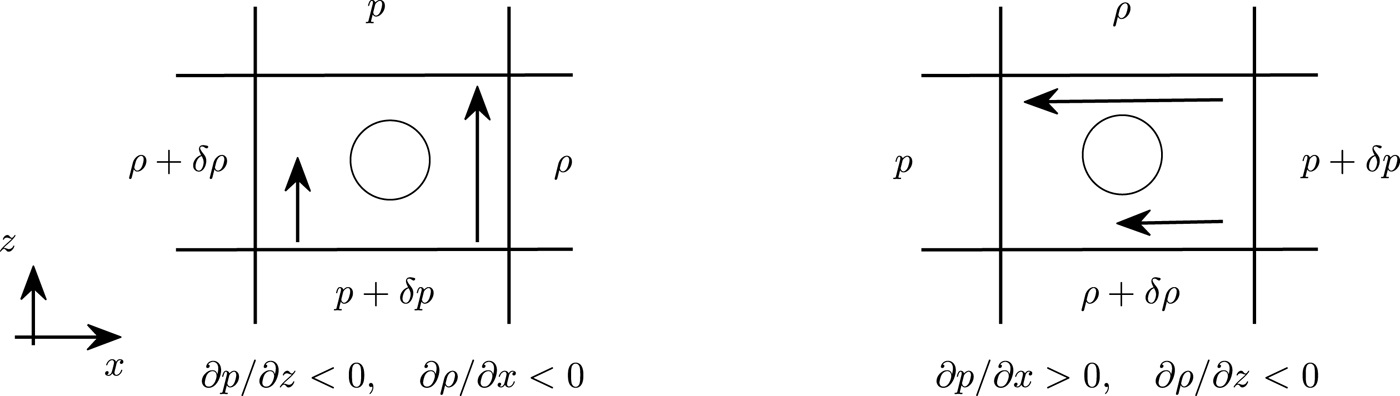
\includegraphics[width=0.9\textwidth]{./figs/lung_figs/baroclinic_schematic} \hfill
 \caption[A schematic of baroclinic torque]{From
    \cite{Heifetz2015}. A hydrostatic force balance upon a particle
    subject to perpendicular pressure and density gradients
    illustrates baroclinic torque on a fluid particle.}
  \label{fig:usbe_lung_baroclinic_schematic}
\end{figure}

For the classical \ac{RMI} setup, a planar shock impinges normally
upon the peaks and troughs of a sinusoidal interface. As the degree of
misalignment varies along the interface, the interface is accelerated
non-uniformly. The direction of the vorticity changes where the
slope of the interface changes. This counter rotation on either side
of interface peaks and troughs entrains nearby fluid causing interface
peaks to accelerate in one direction and troughs to accelerate in the
opposite direction. This results in a ``bubble'' of light fluid
penetrating the heavy fluid, and a ``spike'' of heavy fluid
penetrating the light fluid. How exactly this occurs varies slightly
depending on the relative densities of the two fluids. For the case of
a wave moving from a light fluid into a heavy one, the peaks and
troughs of the interface are initially accelerated to move away from
one another, and the interface perturbation amplitude undergoes growth
exclusively. For the case of a wave moving from a heavy fluid to a
lighter fluid, the peaks and troughs of the interface are accelerated
such that they initially move closer to one another decreasing the
perturbation amplitude. They then pass one another, inverting the
phase of the interface perturbation, and then continue moving in
opposite directions, growing the perturbation amplitude. This process
is illustrated in Figure \ref{fig:rmi_schematic}, which has been
adapted from \cite{Brouillette2002}.
\begin{figure}
  \centering
  \def\svgwidth{0.9\textwidth}
  \import{./figs/lung_figs/}{brouillette_fig3_mod.pdf_tex} \hfill%
  \caption[A schematic view of the \ac{RMI} instability for a
  heavy-light interface]{Adapted from \cite{Brouillette2002}. The
    \ac{RMI} for a heavy-light interface is illustrated. The initial
    condition (left), circulation post wave-interface interaction
    (center), and perturbation growth (right) are shown.}
  \label{fig:rmi_schematic}
\end{figure}

Previous studies of the \ac{RMI} has utilized theory, computation, and
experiments to describe the behavior of the interface after the wave
has passed. \cite{Richtmyer1960} performed the linear stability
perturbation analysis developed by \cite{Taylor1950} for the case of
an impulsive acceleration to create a model for the initial growth of
the interface perturbation. \cite{Meshkov1969} experimentally
confirmed Richtmyer's qualitative predictions, hence the name of the
instability. \cite{Meyer1972} performed numerical simulations of the
\ac{RMI} and found good agreement with Richtmyer for the case of a
shock impinging upon a light-heavy interface. \cite{Fraley1986} used
Laplace transforms in order to find the first analytical solution for
the asymptotic growth rate for a shocked interface between perfect
gases. To describe the late time, nonlinear growth of the
perturbation, \cite{Zhang1997} used single mode perturbation, keeping
many high order terms, to describe the velocity of the bubble and
spike regions of the fluid. \cite{Sadot1998} combined the linear,
impulsive solution with potential flow models of the asymptotic
behavior of the bubble and spike to develop a model for the
perturbation growth that is in good agreement with shock tube
experiments for shocks with Mach numbers Ma=1.3, 3.5. Vortex theory
has also been used to describe the behavior of the
interface. \cite{Jacobs1996} horizontally oscillated a container with
two vertically stratified liquids to obtain standing waves and then
bounced the container off of a coil spring to study the incompressible
\ac{RMI}. The late time evolution of is interface is modeled using a
row of line vorticies to obtain qualitatively similar results to those
experimentally observed, however the late-time growth rate is
underestimated. \cite{Samtaney1994} used shock polar analysis to find
the circulation deposited by a shock on planar and non-planar
interfaces. Their results are validated using and Euler code and found
to be within 10\% of the computed value for $1.0\,<\,$Ma$\,\leq\,1.32$
for all $\rho_2/\rho_1\,>\,1$, and
$5.8\,\leq\,\rho_2/\rho_1\,\leq\,32.6$ for all Ma. This work aims to
add to the current body of work on this topic by investigating
interfaces accelerated by pressure waves within the acoustic regime.

\subsection{Explanation and contributions of the present work}
\label{subsec:usbe_lung_contribution_intro}
We argue that the basic problem setup of the \ac{RMI}, a mechanical
wave impinging upon a material interface, is similar to \ac{DUS} of
the lungs. Accordingly we propose another possible damage mechanism of
\ac{DUS}-induced \ac{LH}. We hypothesize that misalignment between the
pressure gradients in the \ac{DUS} pulses and the sharp density gradients
across the    tissue-air interfaces of the lungs creates a torque around
the alveoli, which deforms and ultimately hemorrhages the alveolar
walls.

The detailed nonlinear interactions between acoustic waves and
perturbed fluid-fluid interfaces does not appear to have been
previously studied in this manner or context. This work is separate
from previous research into the \ac{RMI} as a result of the acoustic
waves being studied. Unlike shock waves, which occur over a few
molecular mean free paths and interact nearly instantaneously,
acoustic waves have a finite spacial wavelength and can occupy a much
larger portion of space. Consequently, their interaction with
interfaces occurs over a longer period of time, the duration of which
depends on a variety of factors including shape and amplitude of the
waveform, the speed of sound in the media, the relative orientation of
the traveling wave and the interface (e.g., the shape of the
interface). This duration can also be thought of in terms of the
relative sizes of the physical features of the interface and the
wavelengths of each feature of the acoustic wave of interest. Simple
\ac{RMI} analysis assumes an impulsive acceleration, and does not
apply to this work because the interface has time to deform throughout its
interaction with the wave. In this work we demonstrate that the finite
duration of the wave-interface interaction can effect the qualitative
behavior of the on interface dynamics because of the interface
deformation that occurs during this period. We will specifically
attempt to address the following questions:
\begin{enumerate} \label{itm:usbe_lung_questions}
\item Are acoustic waves capable of generating sufficient baroclinic
  vorticity at perturbed fluid-fluid interfaces for substantial
  deformations?
\item what is the impact of the acoustic wave properties, such as
  amplitude and wave duration, on the vorticity and interface
  dynamics?
\end{enumerate}

In the remainder of this work, we will first present a simplified
model problem and a set of numerical experiments designed to
investigate the fundamental physics underlying interactions between
acoustic waves and perturbed interfaces between fluids. The simulation
results and related analysis will be presented and discussed first in
the context of the fluid dynamics. We will then draw from these
results to further elaborate on the significance of these results as
they regard to the motivating problem of \ac{DUS}-induced lung
hemorrhage. We will finally end by summarizing the main conclusions
drawn from this work and suggest the next steps to be taken.

%%% Local Variables:
%%% mode: latex
%%% TeX-master: "../../prelim"
%%% End:

\section{Methods} \label{sec:usbe_lung_methods}%
In this section, we describe the set of numerical experiments
performed to investigate the fundamental fluid dynamics associated
with acoustically-accelerated, perturbed liquid-gas interfaces and
\ac{US}-induced \ac{LH}.

\subsection{Problem set-up}
\label{subsec:setup}
\begin{figure}[t]
  \centering
%  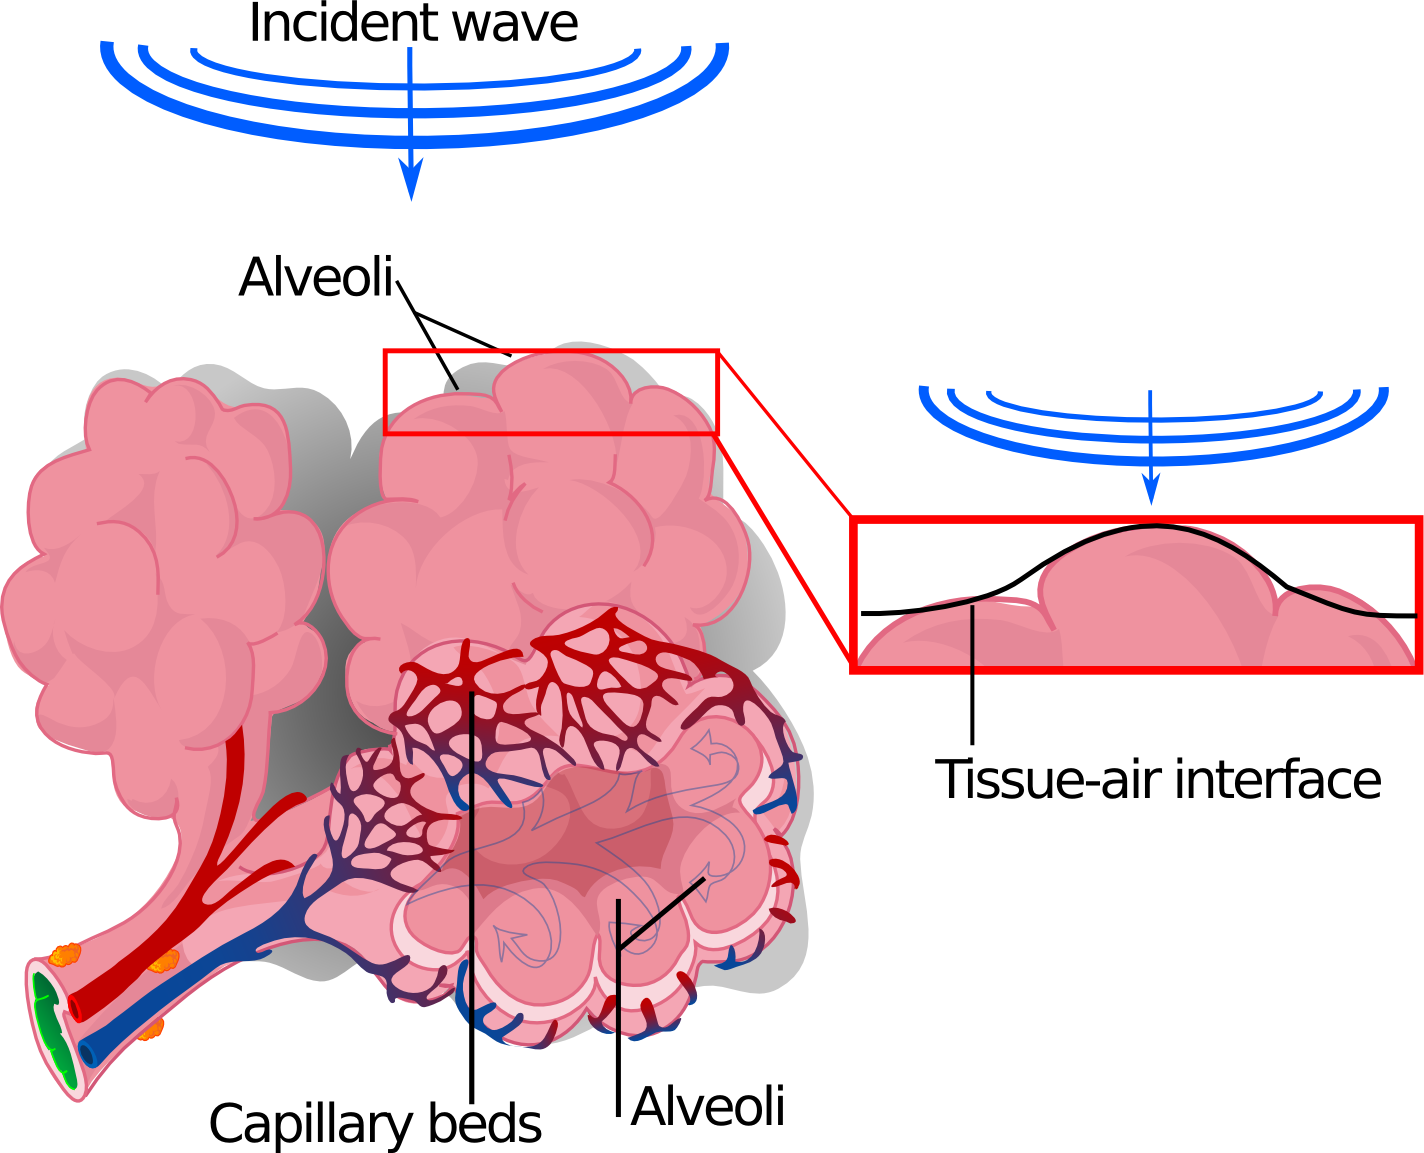
\includegraphics[width=0.48\textwidth]{./figs/lung_figs/Alveolus_US_zoom_diagram.pdf_tex} \hfill

  \def\svgwidth{0.48\textwidth}
  \import{./figs/lung_figs/}{usbe_lung_schematic2.pdf_tex} \hfill%
  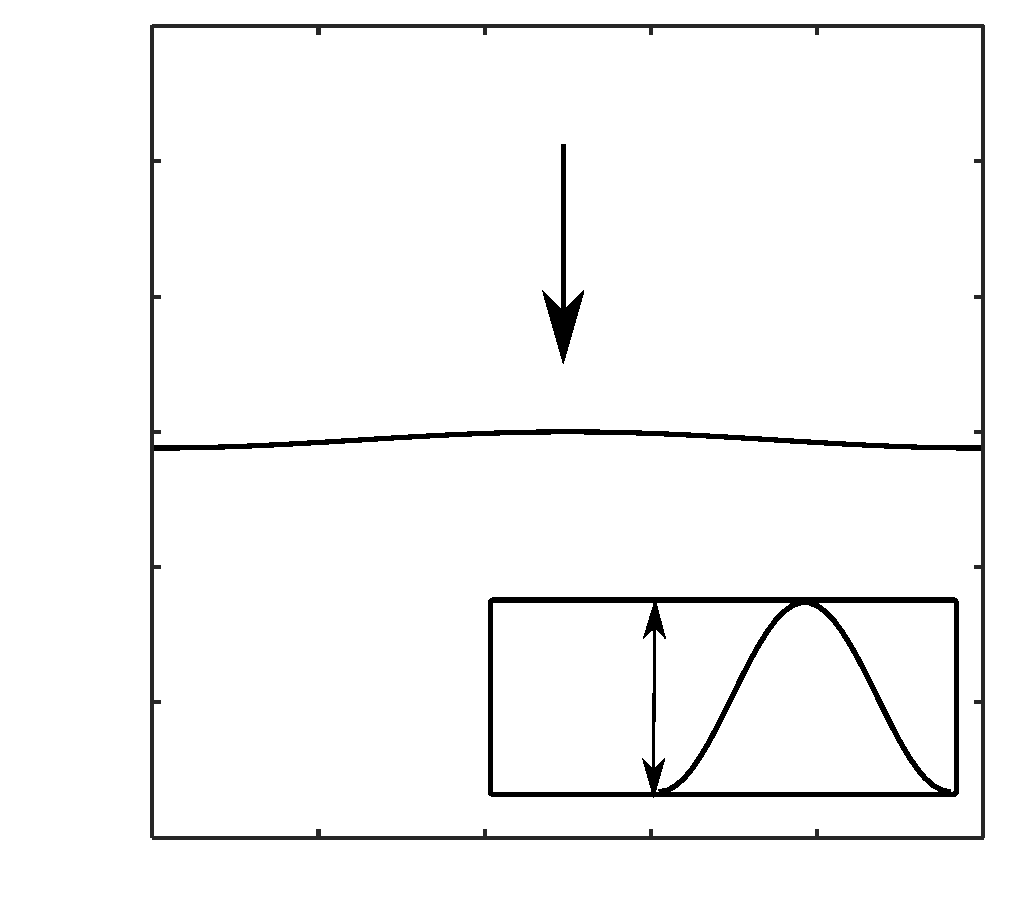
\includegraphics[width=0.48\textwidth]{./figs/lung_figs/usbe_model_schematic} \hfill
  \caption[A schematic view of lung \ac{DUS} and the model problem]{A schematic view of the physical problem (left) is shown next
    to a schematic view of initial setup and boundary conditions of the
    numerical experiments performed (right). A \ac{DUS} pulse impinging
    from tissue onto a pulmonary alveolus is modeled as an acoustic wave
    impinging from water onto a sinusoidally perturbed water-air interface.}
  \label{fig:lung_schematic}
\end{figure}
The experiments are designed to model the physics associated with a
\ac{DUS} pulse propagating from soft lung tissue (modeled as water)
onto a pulmonary alveolus (modeled as air). Accordingly, we consider a
2D, compressible inviscid fluid system in the $xy$-plane with an
acoustic wave impinging from water (top) downward toward air
(bottom). The water-air interface is initially located at the origin
and has a sinusoidal shape with wavelength $\lambda$ and amplitude
$0.03\lambda$ as seen in Figure \ref{fig:lung_schematic}. The width
of the rectangular computational domain is $1\lambda$ such that it is
traversed by a single period of the interface. This interface geometry
is consistent previous studies of the \ac{RMI}
\citep{Brouillette2002}.

To model the \ac{DUS} pulse we consider two different waveforms with
different purposes. We aim to create the first waveform such that the
problem can be analytically studied to understand the relevant
vorticity and interface dynamics. To design this wave, we consider a
typical \ac{US} pulse waveform as one that can be Fourier decomposed
into a sum of sinusoids of varying frequencies and amplitudes. Each
sinusoid can be further broken down into its positive and negative
portions, each consisting of a pressure rise and fall in either
order. We consider only a single rise and fall in pressure and we
simplify further allowing pressure to only rise and fall linearly
(i.e., with constant time derivative). Hence we use an initially
symmetric trapezoidal waves. Each wave is prescribed as an initial
condition in the flow and is composed of three stages, described here
in the order that they encounter the interface. First, compression
occurs. Pressure increases linearly from atmospheric to a maximum of
$p_a=1, 5$, or $10$ MPa gauge pressure. Second, the elevated pressure
$p_a$ remains constant over a fixed distance (or time). Third,
expansion occurs and pressure decreases linearly back to atmospheric
pressure. The pressure rise and fall occur over equal distances
$5\lambda$, such that they have constant, equal slopes
$\pm p_{a}/5\lambda$. Note that this neglects wave distortion due to
acoustically induced changes in sound speed, which we assume to be
small for our purposes. Unless otherwise stated, the period of
constant pressure has length $35\lambda$. Hence the total length $L$
of the incoming trapezoidal wave is $45\lambda$. 

We aim to design the second waveform to closely resemble that of a
typical \ac{DUS} pulse, such that we can compare the associated
interface and vorticity dynamics to those created by the trapezoidal
waveform. The waveform shape is composed of a sinusoidal pressure
modulated by a Gaussian envelope as seen in Figure \ref{fig:p0}),
%
\begin{align} \label{eq:us_waveform}
p(t)=p_a \sin{\left( 2\pi f \left[ t-t_0\right]\right)}
\exp{\left(-\frac{t-t_0}{FWHM/\left(2\sqrt{2\ln{\left(2\right)}}\right)}\right)}.
\end{align}
%
Here $p(t)$ is the pulse pressure as a function of time, $p_a$ is the
maximum acoustic pressure, $f$ is the frequency in Hz, $t$ is time,
$t_0$ is a time offset, and $FWHM$ is the full width at half maximum
amplitude for the Gaussian envelope. The presented \ac{DUS}-like pulse
waveform is given as a function of time, as is typical of \ac{US}. The
speed of sound in water is used to convert this to a spatial waveform
for the initial condition.

we assume a typical alveolar length scale
$\lambda=100 \, \mu$m. For the wave initially in water, (c=$1500$
m/s), we find an equivalent acoustic pulse duration of our waveform is
$3 \, \mu$s.  This is within the range of typical \ac{US} pulse
durations in clinical imaging \citep{Edelman2005} and relevant
research \citep{Obrien2006b}.
%
\begin{figure}% 
  \centering%
  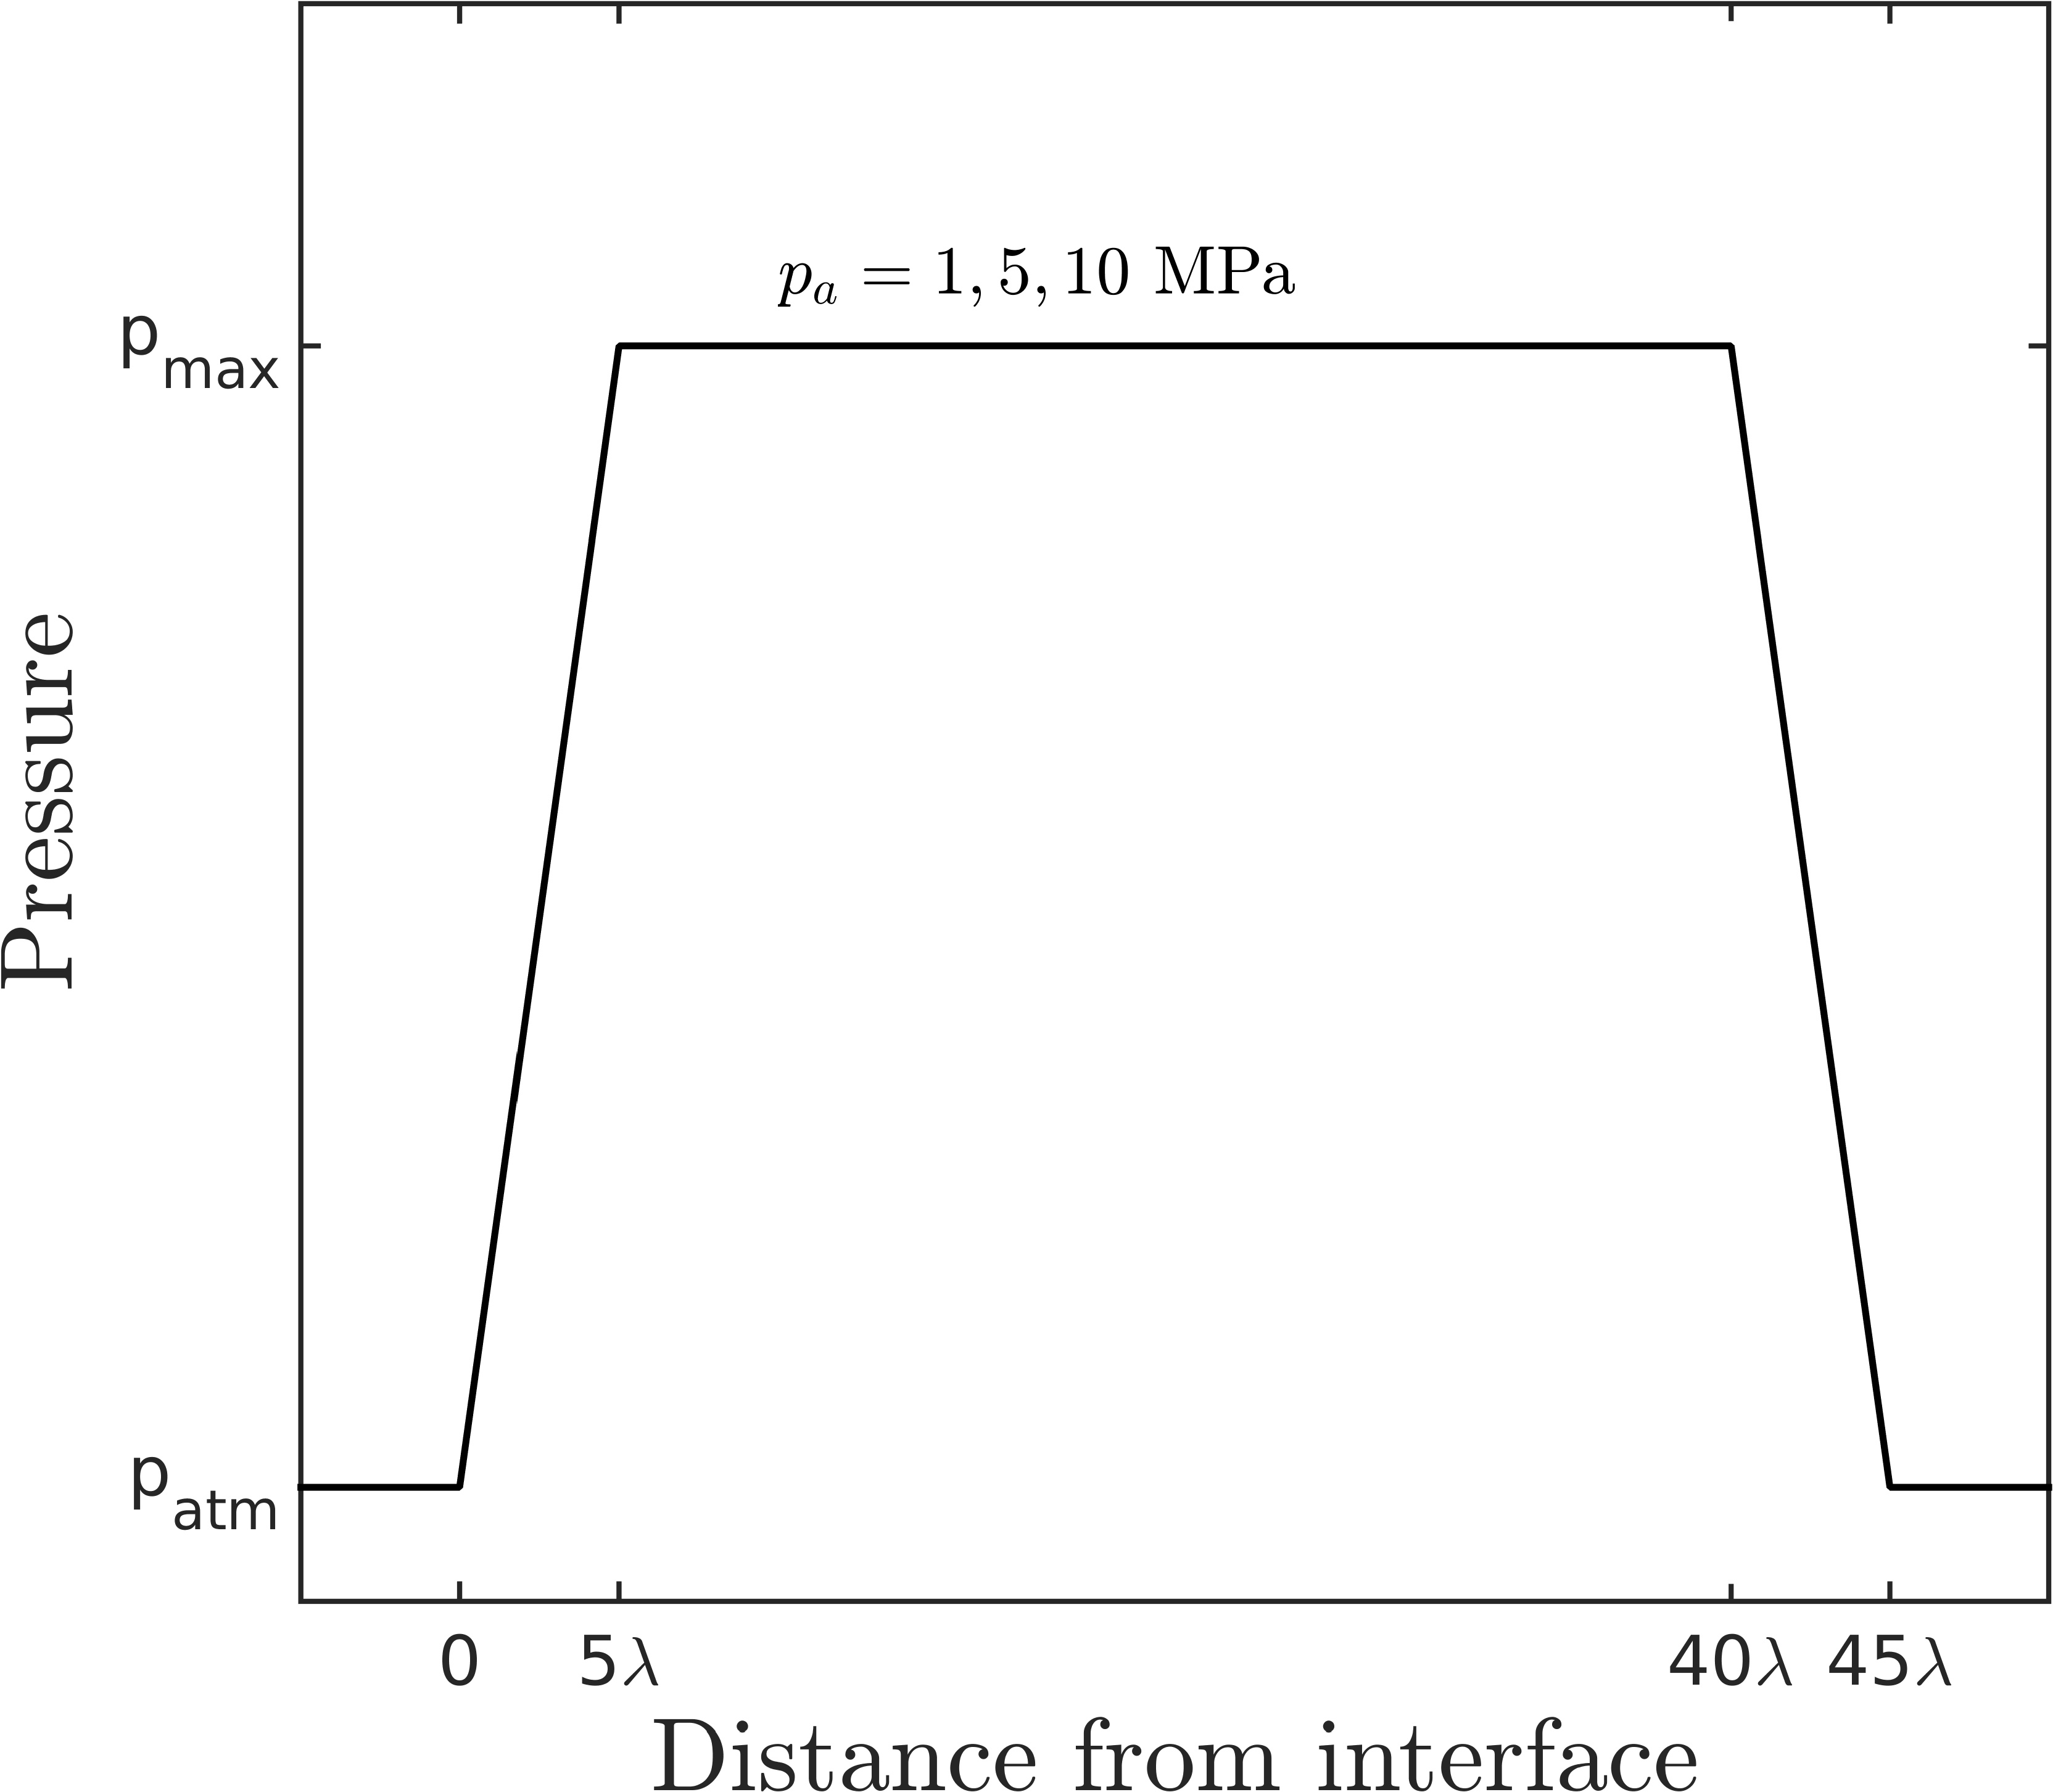
\includegraphics[width=0.47\textwidth]{./figs/lung_figs/p0_vs_y}%
  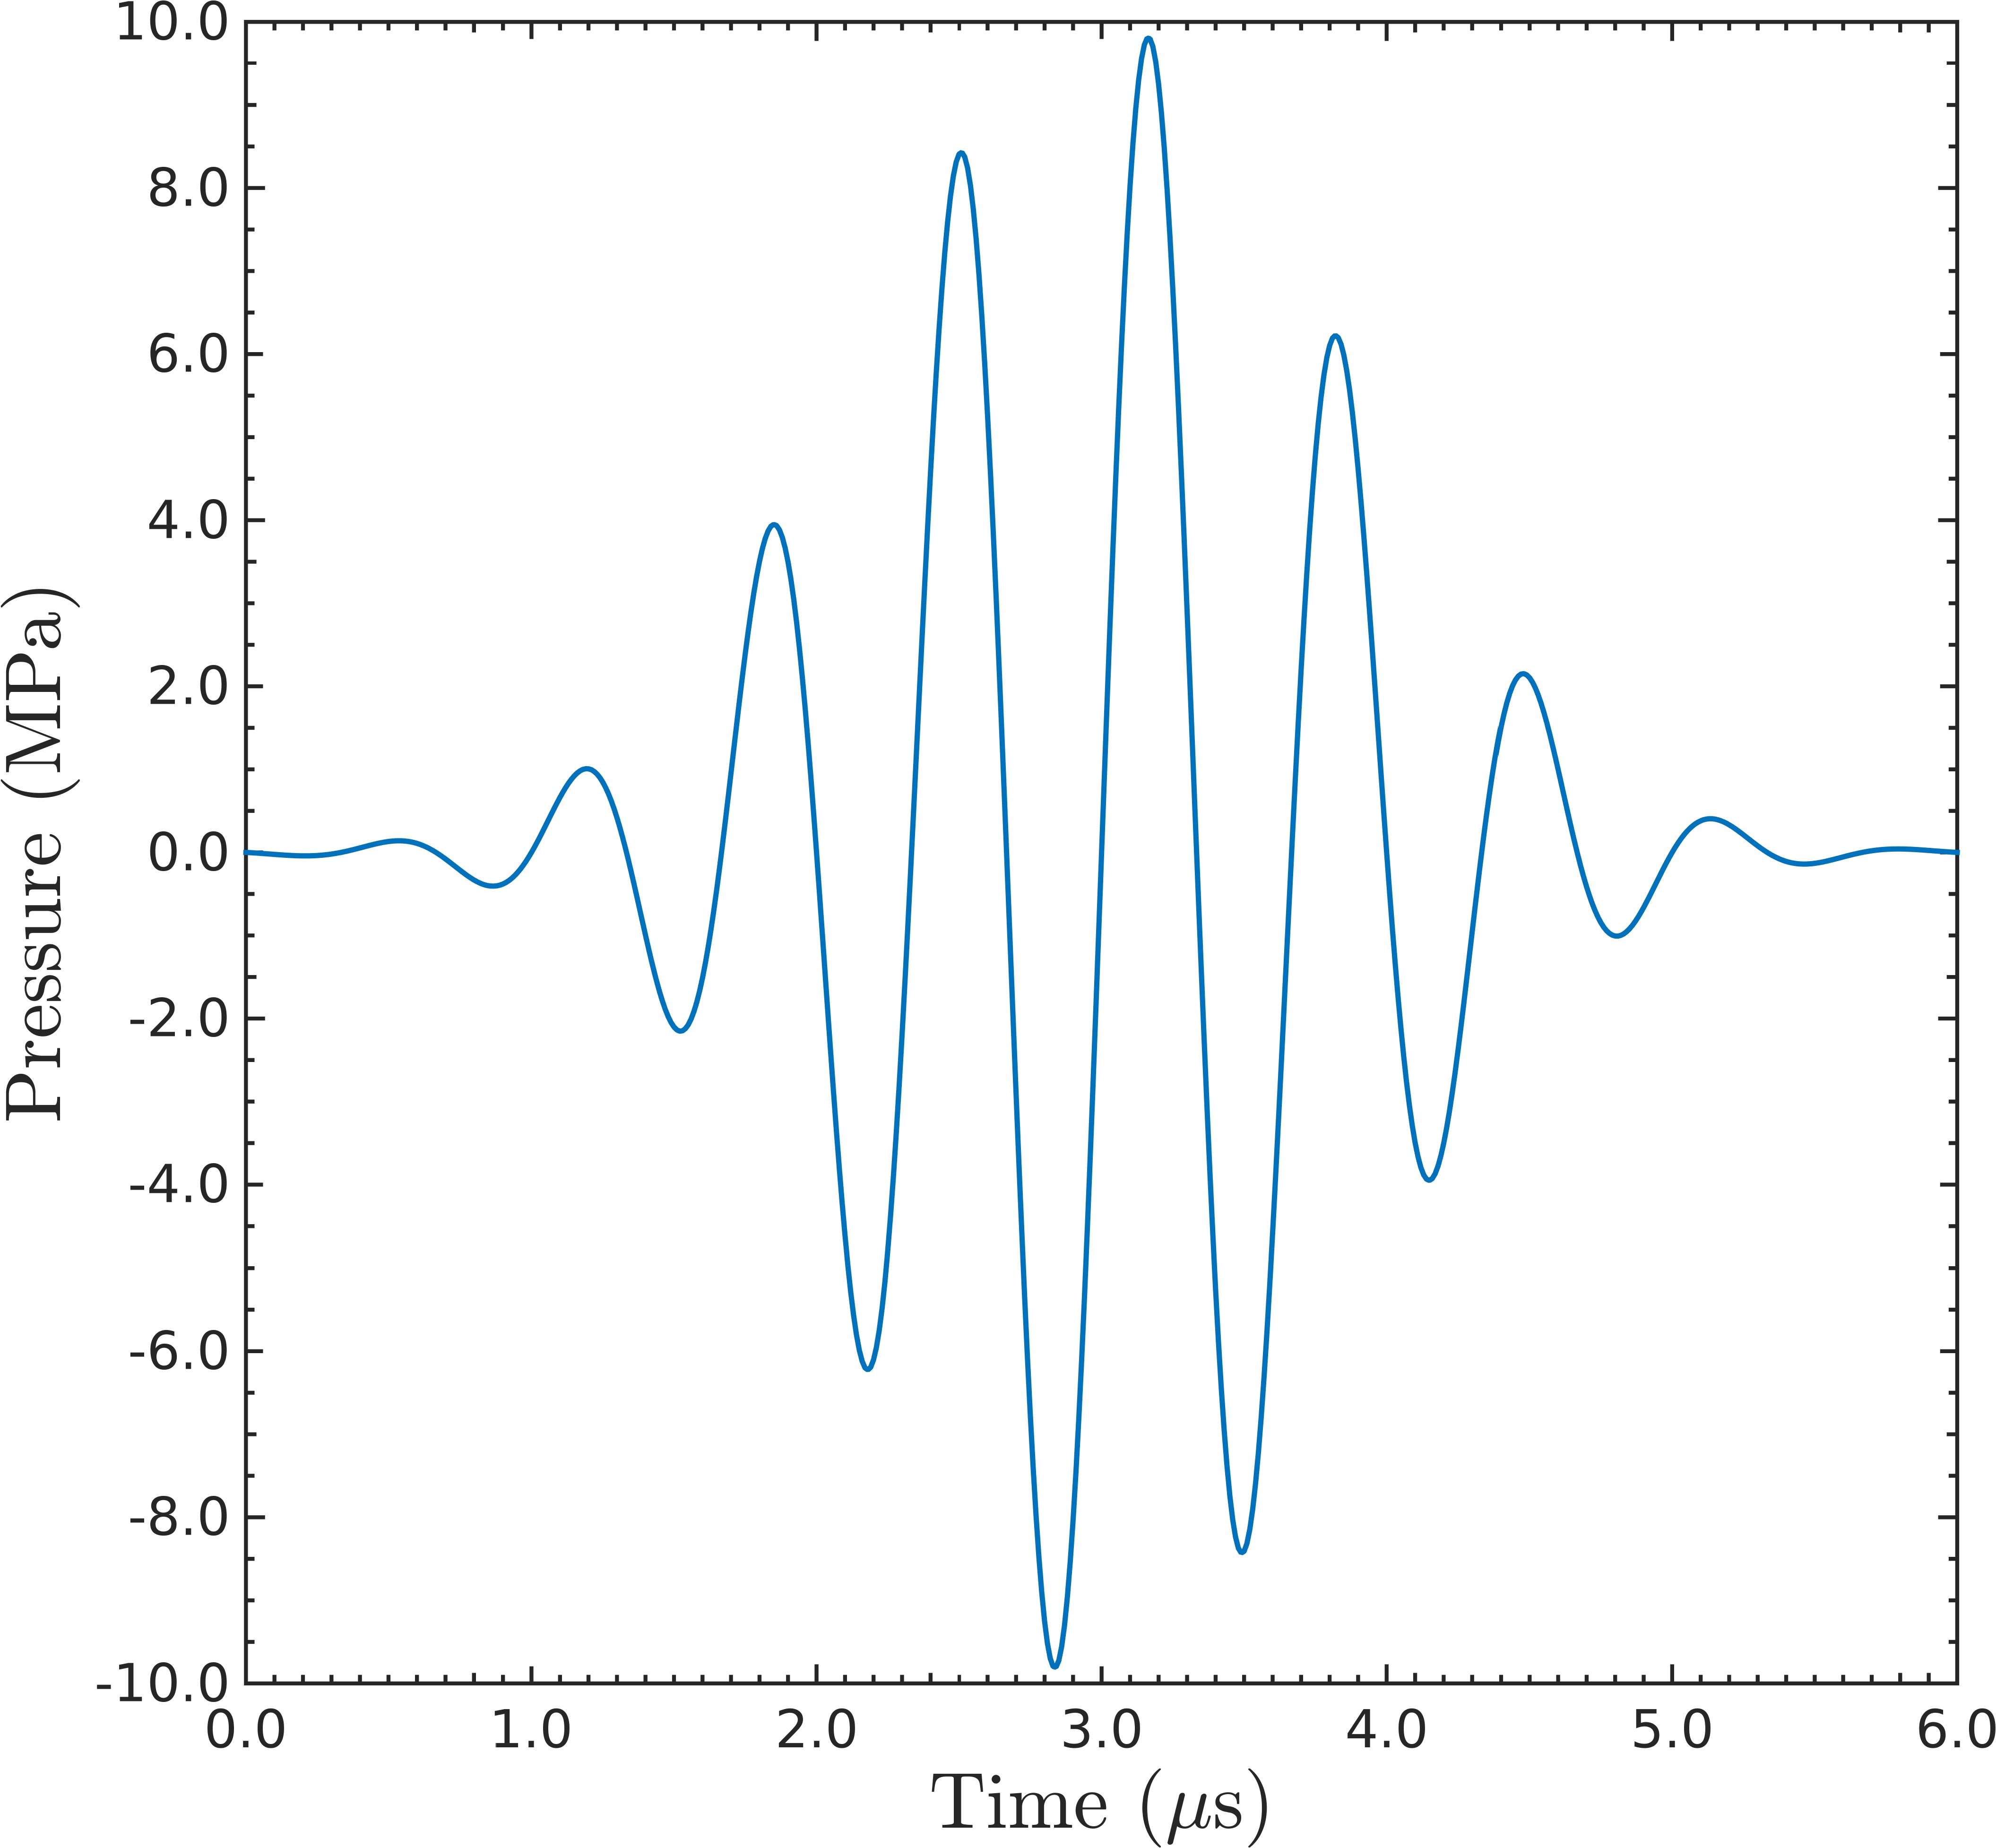
\includegraphics[width=0.47\textwidth]{./figs/lung_figs/p0_vs_t_us}%
  \caption[Trapezoidal and \ac{DUS} pulse waves]{The initial pressure in the domain. The trapezoidal wave
    pressure is shown as a function of distance from the interface
    (Left). A \ac{DUS}-like pulse wave is used for comparison
    (Right).}%
  \label{fig:p0}
\end{figure}
%
\subsection{Governing equations}
The governing equations describing the dynamics \ac{US} lung
interaction are conservation of mass, momentum, and energy for a
compressible, viscoelastic material. In the present work we neglect
elastic and viscous effects to arrive at the Euler equations of fluid
motion, which we nondimensionalize by the density $\rho$ and speed of
sound $c$ of air.  For our setup we model the tissue as water and
alveolus as air and the \ac{DUS} pulse as a trapezoidal pressure
waveform. Hence we solve the Euler equations to simulate simplified
trapezoidal acoustic waves propagating from water towards a
sinusoidally perturbed water-air interface. The interface and
vorticity dynamics are studied.

It is worth noting that the Euler equations are length scale invariant, and
thus no inherent physical length scale exists in the equations that we
solve. Hence all length scales hereafter will be considered relative
to an interface perturbation wavelength $\lambda$. Within the context
of the \ac{DUS}, $\lambda$ can be thought of as a typical length scale
of an alveolus.

We solve the dimensionless Euler equations of compressible, inviscid
fluid motion in two dimensions ($x,y$),
%
\begin{subequations} \label{eq:euler}%
  \begin{align}% 
    \frac{\partial \rho}{\partial t} + \frac{\partial \left(\rho u\right)}{\partial x} + \frac{\partial \left(\rho v\right)}{\partial y} = 0,\\
    \frac{\partial \rho u}{\partial t} + \frac{\partial}{\partial x}\left( \rho u^2+p\right)  + \frac{\partial}{\partial y}\left( \rho uv\right) = 0,\\
    \frac{\partial \rho v}{\partial t} + \frac{\partial}{\partial x}\left( \rho uv\right)  + \frac{\partial}{\partial y}\left( \rho v^2+p\right) = 0,\\
    \frac{\partial E}{\partial t} + \frac{\partial}{\partial x}\left[u\left(E+p\right)\right] + \frac{\partial}{\partial y}\left[v\left(E+p\right)\right] = 0,
  \end{align}%
\end{subequations}%
%
where $t$ is time, $\rho$ is density, $p$ is the pressure, $u$ and $v$
are the velocity components in the $x$ and $y$ directions
respectively, and $E$ is the total energy. We use the density and
sound speed of air at 300 K to nondimensionalize the system. It is
worth noting that the Euler equations are length scale invariant, and
thus no inherent physical length scale exists in the equations that we
solve. Hence all length scales hereafter will be considered relative
to an interface perturbation wavelength $\lambda$.

To close the system, we solve a stiffened equation of state which
relate the total energy to the pressure and velocity in the flow, such
that,
% 
\begin{align} \label{eq:stiffened_eos}%
  E=\frac{\rho\left(u^2+v^2\right)}{2} + \frac{p+\gamma B}{\gamma-1}.
\end{align}
%
Here $B$ is a measure of liquid stiffness. For perfect gases, such as
is our treatment of air, $\gamma$ is the specific heats ratio and
$B=0$. The sound speed in our simulations is calculated based on the
following relationship, derived from the stiffened equation of state.
%
\begin{align}
  c = \sqrt{\frac{\gamma\left(p+B\right)}{\rho}}.
\end{align}
%
While physical diffusion is not considered in this setup, numerical
diffusion does occur at the water-air interface, creating a mixed
region between the two fluids. The numerical treatment of the
diffusion layer at the interface for the initial condition is such
that the density has an exponential profile \citep{Latini2007}, which
is used to get the mass fraction and molecular weight fields in the
mixed region. Which then used to determine the other material
parameters in the mixed region in a thermodynamically consistent
fashion.

To solve for
the material parameters in the mixed region and prevent spurious
pressure oscillations at the interface, two additional advection
equations are solved for $\gamma$ and $B$.
\begin{subequations} \label{usbe_lung_eosvar_advection}%
\begin{align}% 
\frac{\partial}{\partial t}\left(\frac{\gamma B}{\gamma-1}\right)+\vec{u}\frac{\partial}{\partial x}\left(\frac{\gamma B}{\gamma-1}\right) = 0,\\
\frac{\partial}{\partial t}\left(\frac{1}{\gamma-1}\right)+\vec{u}\frac{\partial}{\partial x}\left(\frac{1}{\gamma-1}\right) = 0. 
\end{align}%
\end{subequations}%
This implementation is consistent with the works of \cite{Abgrall1996,
  Shyue2001, Beig2015}. Details of this implementation are explained
by \cite{HenrydeFrahan2015}.
%
The dimensional and dimensionless values of each fluid property can be
found in tables \ref{tab:usbe_lung_dimensional_parameters} and
\ref{tab:usbe_lung_dimensionless_parameters} respectively.
% 
\begin{table}[bp]%
  \begin{center}
    \caption{Dimensional properties of air and water used in simulations.}
    \label{tab:usbe_lung_dimensional_parameters}%
    \begin{tabularx}{0.75\textwidth}{| X | X | X | X | X |}
      \hline
      & Density, $\rho^*$ (kg/m$^3$) & $\gamma$ & $B^*$ (Pa)  & $c^*$ (m/s) ($p$=$1$ atm) \\ \hline
      Air   & 1.18                        & 1.4      & 0         & 347.2     \\ \hline
      Water & 996                           & 5.5      & 492115000 & 1648.7     \\ \hline
      \multicolumn{5}{l}{\small $^*$ indicates dimensional parameter}
    \end{tabularx}
  \end{center}
\end{table}%
\begin{table}[bp]%
  \begin{center}
    \caption{Dimensionless properties of air and water used in simulations.}
    \label{tab:usbe_lung_dimensionless_parameters}%
    \begin{tabularx}{0.75\textwidth}{| X | X | X | X | X |}
      \hline
      & Density, $\rho$ & $\gamma$ & $B$ & $c$ \\ \hline
      Air   & 1                          & 1.4      & 0         & 1          \\ \hline
      Water & 846.6                      & 5.5      & 3469.1    & 4.75       \\ \hline
      \multicolumn{5}{l}{\small Parameters are nondimensionalized by the density and sound speed of air. }
    \end{tabularx}
  \end{center}
\end{table}
%
\subsection{Numerical methods}%
\label{subsec:numerical_methods}%
To solve the governing equations, we implement a third-order accurate
\ac{DG} scheme in space and a fourth-order accurate, adaptive
Runge-Kutta method to march forward in time
\citep{HenrydeFrahan2015}. Roe solver is used to calculate flux in an
out of each cell in a way that handles discontinuities and keeps the
interface sharp. As previously stated, the computational domain width
($x$-direction) is $\lambda$. The domain length ($y$-direction) is
80$\lambda$. The grid resolution is 100 points per $\lambda$ unless
otherwise stated. To minimize artificial reflections, we use inflow
and outflow boundary conditions at the top and bottom of the domain,
and implement geometric grid stretching in the vertical direction for
the top and bottom-most 10$\lambda$ segments of the grid. Periodic
boundary conditions are used at the left and right edges of the
domain.

%%% Local Variables:
%%% mode: latex
%%% TeX-master: "../../prelim"
%%% End:

\section{Analysis}%
\label{sec:usbe_lung_analysis}%
We perform analysis to make quantifiable predictions about the
vorticity and interface dynamics. The results of these
analyses are compared with the results of our numerical experiments in
section \ref{sec:usbe_lung_results}.

To better understand the source of circulation within our problem we
look to the vorticity generation equation for a 2D, inviscid fluid
system,
\begin{align} \label{eq:vorticity_euler}
  \frac{\partial \vec{\omega}}{\partial t}+\left(\vec{u}\cdot\nabla\right)\vec{\omega} =% 
  - \vec{\omega}\left(\nabla\cdot\vec{u}\right) + \frac{\nabla\rho\times\nabla p}{\rho^2}.%
\end{align}
Each term in equation \eqref{eq:vorticity_euler} represents a
different physical mechanism by which the vorticity $\vec{\omega}$ is
changing. The terms on the left-hand side of the equation represent
changes in the existing vorticity field and the terms on the right
represent vorticity sources and sinks. The first term on the left
represents the total change of vorticity at a location in the flow
field with respect to time. The second term on the left represents the
advection of vorticity within the field. The first term on the right
describes changes in vorticity due to compressibility. The last term
on the right is the baroclinic term which represents vorticity
generated by the misalignment of the pressure and density gradients in
the flow. We seek to understand the relative importance of these
mechanisms on the dynamics of the acoustically driven interface.

\subsection{Order of magnitude analysis of vorticity generation mechanisms}
To quantifiably compare the various mechanisms by which vorticity
changes within the flow, we recognize that any vorticity generated
must be a result of acoustic energy being converted to kinetic
energy. As the only mechanism for this to occur in an inviscid fluid
without pre-existing vorticity is baroclinic, we require misaligned
density and pressure gradients. Hence we choose to perform our
analysis at the water-air interface during the period in which the
interface is interacting with the incoming wave. For simplicity, we
narrow this down to only consider the period in which the incoming
compressive portion of the wave encounters the interface. As this
interaction occurs quickly, over an approximate time span
$\Delta t_a\approx5\lambda/c_{w}$, we assume that the interface is
static and remains undeformed from its initial state during this
interaction. We will show in section \ref{sec:usbe_lung_results} that
this assumption is reasonable for the cases considered. Having now
established the point at which the analysis is to be performed we
evaluate the order of magnitude of the compressible, advective, and
baroclinic terms of the vorticity generation equation
\eqref{eq:vorticity_euler}. We note that the advective term is not a
true source of vorticity, but is useful in understanding the change of
vorticity at a given time and location within the flow.

In our evaluation of the order of magnitude of the individual terms of
the vorticity generation equation \eqref{eq:vorticity_euler}, we treat
gradient, curl, and divergence terms of any arbitrary quantity $f$
such that $\nabla f= \orderof{\left|\Delta f\right|/\Delta L}$,
$\nabla\cdot f=\orderof{\left|\Delta f\right|/\Delta L}$, and
$\nabla\times f=\orderof{\left|\Delta f\right|/\Delta L}$. Here
$\Delta f$ is a change in $f$ over a characteristic length scale
$\Delta L$. Because the only motion in the flow is generated by the
acoustic wave. Accordingly, we consider acoustic pressure, velocity,
and density perturbations such that $\Delta p=\Delta p_a$,
$\Delta \vec{u}=\Delta \vec{u}_a$, and $\Delta \rho=\Delta \rho_a$,
and use acoustic relations to relate these quantities
\citep{Anderson1990},
\begin{align}%
  \label{eq:acoustic_relations}%
  \Delta p_a=\pm\Delta u_a \rho c=c^2\Delta \rho_a.%
\end{align}
Additionally, to evaluate the expressions in this section we use the
values in in tables \ref{tab:usbe_lung_dimensional_parameters} and
\ref{tab:usbe_lung_dimensionless_parameters} consider our base
trapezoidal wave case where $p_a = \Delta p_a = 10$ MPa. The length
scale associated with the acoustic wave is the initial length of the
pressure rise $\Delta L_a=5\lambda$. The initial interface length
scale $\Delta L_I$, defined as the thickness of the thickness of the
mixed layer from 0.05 to 0.95 volume fraction is estimated as
$\Delta L_I \approx 0.05\lambda$. We approximate the order of theta
based on its average value along a half-wavelength of the interface
for our initial condition $a_0=0.03\lambda$ such that
$\overline{\abs{\theta}}\approx0.12$.

To assess the baroclinic contribution to vorticity, we write the cross
product of the density and pressure gradients as
$\abs{\nabla \rho} \abs{\nabla p} \sin{\left(\theta\right)}$. Here
$\theta$ is the angle between the acoustic pressure gradient, treated
as constantly in the $\plus y$-direction, and the direction of the
density gradient which we treat as the outward normal direction to the
interface. For $a_0/\lambda<<1$, we can approximate
$\sin{\left(\theta\right)}\approx\theta$ at the interface. The density
gradient due to the water-air interface is far greater than that due
to the acoustic wave. As such we use the change in density across the
interface $\Delta \rho_I$ and associated length scale $\Delta L_I$ to
write the density gradient. The pressure change is a result of the
acoustic wave, and as such we use the acoustic pressure change
$\Delta p_a$ and associated length scale $\Delta L_a$ to express the
pressure gradient. And thus we write the order of magnitude of the
baroclinic vorticity generation term at the interface,
\begin{align}
  \label{eq:baroclinic_vorticity}%
  \norm{\frac{\nabla\rho\times\nabla p}{\rho^2}} = \orderof{\frac{\abs{\Delta \rho_I}}{\abs{\Delta L_I}}\frac{\abs{\Delta p_a}}{\abs{\Delta L_a}}\frac{1}{\abs{\rho}^2}\abs{\theta}}.%
\end{align}

In the evaluation of the compressible and advective terms we consider
two possible cases for the evaluation of the vorticity, based on
whether the dominant vorticity arises from the acoustic flow-field or
is baroclinically generated. Thus we will ultimately treat
$\vec{\omega}$ as either the curl of the acoustic velocity field
$\vec{\omega}=\nabla\times\vec{u}$ or the integral of the baroclinic
vorticity generation term \eqref{eq:baroclinic_vorticity}, treated as
constant, over the characteristic time of the pressure rise
$\Delta t_a\approx\Delta L_a/c_w$.

We first consider the case in which vorticity is predominately a
product of the acoustic velocity field such that the approximate order
of magnitude of the compressible contribution to vorticity generation
is expressed as
\begin{align}
  \label{eq:compressible_vorticity}%
  \norm{-\vec{\omega}\left(\nabla\cdot\vec{u}\right)} = \orderof{\left[\frac{\abs{\Delta u_a}}{\abs{\Delta L_a}}\right]^2},%
\end{align}
and for the advective contribution we find
\begin{align}
  \label{eq:advective_vorticity}%
  \norm{\left(\vec{u}\cdot\nabla\right)\vec{\omega}} = \orderof{\left[\frac{\abs{\Delta u_a}}{\abs{\Delta L_a}}\right]^2}.%
\end{align}
We note that from this analysis, we expect the advective and
compressible vorticity effects to be of the same order during
considered period and will treat them as such for the remaining
analysis.

Now, to compare the relative importance of the baroclinic and
compressible (or advective) contributions to vorticity for this case
we will look at the ratio of the two vorticity generation
approximations. We divide equation \eqref{eq:baroclinic_vorticity} by
equation \eqref{eq:compressible_vorticity} use
\eqref{eq:acoustic_relations} to express acoustic quantities in terms
of the density perturbation $\Delta \rho_a$ and simplify,

\begin{align} \label{eq:vorticity_comparison_broke}
%\left(\frac{\partial\omega}{\partial t}\right)_{\text{baroclinic}} / \left(\frac{\partial \omega}{\partial t}\right)_{\substack{\text{compressible/}\\\text{advective}}} =&%
\frac{\norm{\frac{\nabla\rho\times\nabla p}{\rho^2}}}{\norm{-\vec{\omega}\left(\nabla\cdot\vec{u}\right)}} =&%
\orderof{\left(\frac{\abs{\Delta \rho_I}}{\abs{\Delta L_I}}\frac{\abs{\Delta p_a}}{\abs{\Delta L_a}}\frac{1}{\abs{\rho}^2}\abs{\theta}\right) /%
\left( \left[\frac{\abs{\Delta u_a}}{\abs{\Delta L_a}}\right]^2 \right)}\nonumber\\%
%
=&\orderof{\left[\frac{\abs{\Delta \rho_I}}{\abs{\Delta L_I}}\frac{\abs{\Delta \rho_a}}{\abs{\Delta L_a}}\frac{\abs{c}^2}{\abs{\rho}^2}\abs{\theta}\right] /
\left[\frac{\abs{c}}{\abs{\rho}}\frac{\abs{\Delta \rho_a}}{\abs{\Delta L_a}}\right]^2}\nonumber\\%
%
=&\orderof{\frac{\abs{\Delta \rho_I}/\abs{\Delta L_I}}{\abs{\Delta \rho_a}/\abs{\Delta L_a}} \abs{\theta} }.
%=&\orderof{\abs{\theta}\frac{\abs{\Delta \rho_I}}{\abs{\Delta L_I}} / \frac{\abs{\Delta \rho_a}}{\abs{\Delta L_a}}}.
\end{align}
Evaluating the right-hand side of
\eqref{eq:vorticity_comparison_broke} using the previously described
approximations and values we find that the ratio of baroclinic
vorticity and compressible contributions to vorticity to be of order
$\orderof{10^3}$.

As the previous result would suggest that baroclinic vorticity
generation is strongly dominant, we must check the result by again
evaluating the compressible and advective contributions to vorticity
generation, using an expression for vorticity based on the time
integration of \eqref{eq:baroclinic_vorticity},
\begin{align}
  \label{eq:compressible_advective_vorticity}%
\norm{-\vec{\omega}\left(\nabla\cdot\vec{u}\right)}\sim \norm{\left(\vec{u}\cdot\nabla\right)\vec{\omega}} = %
\orderof{\frac{\abs{\Delta u_a}}{\abs{\Delta L_a}} \frac{\abs{\Delta \rho_I}}{\abs{\Delta L_I}}\frac{\abs{\Delta p_a}}{\abs{\Delta L_a}}\frac{1}{\abs{\rho}^2}\abs{\theta}\frac{\abs{c}}{\abs{\Delta L_a}}}.%
\end{align}
%
Again, comparing the relative importance of the baroclinic and
compressible (or advective) contributions to vorticity as we did before,
\begin{align} \label{eq:vorticity_comparison}
\frac{\norm{\frac{\nabla\rho\times\nabla p}{\rho^2}}}{\norm{-\vec{\omega}\left(\nabla\cdot\vec{u}\right)}} = \frac{c}{\abs{\Delta u_a}} = \frac{\rho}{\abs{\Delta \rho_a}}%
\end{align}
Now evaluating this expression we expect that the relative contribution of
baroclinic to compressible/advective vorticity generation is
approximately of order $\orderof{10^2}$ at the end of the
compression-interface interaction.

Comparing the evaluations of expressions
\eqref{eq:vorticity_comparison_broke} and
\eqref{eq:vorticity_comparison} we expect two things. First, that
baroclinicity will be the dominant physical mechanism by which
circulation is generated. Hence, we expect
that \label{eq:vorticity_comparison_broke} is likely to overestimate
the dominance of baroclinic vorticity after a small amount of
baroclinic vorticity has been generated. Second, we expect the ratio
of the baroclinic to compressible contributions to vorticity
generation will range from $\orderof{10^3}$ to $\orderof{10^2}$ during
the compression-interface interaction.

\subsection{Comparison of vorticity generation in air and water}
Having established that the dominant source of vorticity is
baroclinicity we now aim to determine where this vorticity will
generated within the mixed region of the interface. Specifically, we
aim to compare the order of baroclinic vorticity generation from
equation \eqref{eq:baroclinic_vorticity} in pure water and air. As
this can already be evaluated in water from what we have provided up
to this point, we will focus on evaluation of the order of baroclinic
vorticity generation in air, from equation
\eqref{eq:baroclinic_vorticity}. Throughout the analysis we will
denote the properties of the incoming wave and water with a subscript
$-$, and the transmitted wave and air with a subscript $+$. For water,
we will use the values for
$\Delta \rho_I, \Delta L_I, \Delta \rho_a, \Delta L_a$ and $\theta$
defined in the previous section based on our initial condition. Our
treatment of the density gradient at the interface will remain
unchanged for evaluation in air such that
$\Delta \rho_I^-=\Delta \rho_I^+$ and $\Delta L_I^-=\Delta L_I^+$.

As a portion of the acoustic wave is transmitted into air, it
undergoes several physical changes relative to the incident wave. To
describe the properties of the transmitted wave in air we will borrow
techniques from linear acoustics. To find the pressure change in the
transmitted compression wave $\Delta p_a^+$, we recognize that
$a_0/\lambda<<1$ and treat the incoming wave as a plane wave impinging
normally on a flat material interface such that
$\Delta p_a^+=\bs{T} \Delta p_a^-$, where $\bs{T}$ is the acoustic
transmission coefficient,
$\bs{T}=2\rho^+ c^+/\left(\rho^+ c^+ + \rho^- c^- \right)$
\citep{Kinsler1982}. For our water-air interface
$\bs{T}\approx4.97\times10^{-4}$. Because of the strong impedance
mismatch between fluids, the acoustic wave is almost entirely
reflected, decreasing the pressure gradient of the transmitted wave
relative to the incident wave. Because of the drop in sound speed
across the interface, the transmitted wave is compressed into a
smaller physical area (i.e., the wavelength decreases) relative to the
incoming wave, such that $\Delta L_a^+=\Delta L_a^- (c^+/c^-)$. This
effect increases the pressure gradient in the transmitted wave. To
evaluate $\theta^+$, we utilize Snell's law which states that
$c^-\sin{(\theta^-)}=c^+\sin{(\theta^+)}$. Tedious, but simple
geometric arguments can be used to show that because $a_0/\lambda<<1$
it is also true that $\theta^-<<1$. Thus we use the small angle
approximation of $\sin$ to find that
$\theta^+\approx\theta^-(c^+/c^-)$. We note that this decreases the
misalignment between the pressure and density gradients in air, and
quantitatively approximately cancels the increase in pressure gradient
due to the decrease in wavelength of the transmitted wave.

To determine where the vorticity will be generated at the interface,
we consider equation \eqref{eq:baroclinic_vorticity} in air and water
and write the ratio to find
\begin{align}%
\label{eq:baroclinic_air_water}%
%\left(\frac{\partial\omega}{\partial t}\right)_{\substack{\text{baroclinic}\\\text{air}}} / \left(\frac{\partial\omega}{\partial t}\right)_{\substack{\text{baroclinic}\\\text{water}}}%
\frac{\norm{\frac{\nabla\rho\times\nabla p}{\rho^2}}_{air\quad}}{\norm{\frac{\nabla\rho\times\nabla p}{\rho^2}}_{water}}
=&\orderof{\frac{\left[\frac{\abs{\Delta \rho_I^+}}{\abs{\Delta L_I^+}}\frac{\abs{\Delta p_a^+}}{\abs{\Delta L_a^+}}\frac{1}{\abs{\rho^+}^2}\abs{\theta^+}\right]}
{\left[\frac{\abs{\Delta \rho_I^+}}{\abs{\Delta L_I^+}}\frac{\left(\abs{\Delta p_a^+}/\abs{\bs{T}}\right)}{\abs{\Delta L_a^+}\left(\abs{c^+}/\abs{c^-}\right)}\frac{1}{\abs{\rho^-}^2}\left(\abs{c^+}/\abs{c^-}\right)\abs{\theta^+}\right]}},\nonumber\\%
=&\orderof{\abs{\bs{T}}\left(\frac{\abs{\rho^-}}{\abs{\rho^+}}\right)^2}.%
\end{align}
For our water-air interface, we evaluate equation
\eqref{eq:baroclinic_air_water} to find that the ratio of baroclinic
vorticity generation in air to that in water would be of order
$\orderof{10^2}$. While this result considers vorticity generation in
pure air and water, as opposed to the mixed fluid region relevant to
this work, it provides a useful upper bound on the change we expect in
the vorticity across the interface. Additionally, this result suggests
that for the mixed water-air region, where the strongest density
gradient exists, vorticity generation is likely to occur in areas with
a lower volume fraction of water (i.e., gas-dominated fluid).

\subsection{Considerations of circulation}
In order to verify our analyses numerically we will consider not the
vorticity generation, but rather the circulation and circulation
generation as functions of time. As circulation is a global quantity
of vorticity integrated over a region, it is more practical to compare
to our numerical experiments. The expressions previously obtained for
estimates of vorticity generation can be integrated in space to obtain
integral expressions for circulation generation. As the expressions
derived were approximate and spatially independent, we expect that the
approximate vorticity relationships found in this section can be
extended to considerations of the circulation. For instance, based on
the results of equation \eqref{eq:vorticity_comparison} we expect the
baroclinic circulation generation in the left or right half-domain to
be $\orderof{10^2}$ larger than the compressible and advective terms
toward the end of interaction between the interface and the acoustic
compression.

To access this, we integrate equation \eqref{eq:vorticity_euler} over
the half-domain, $A_R$, to get
\begin{align} \label{eq:circulation_generation}
  \left(\frac{\partial \Gamma}{\partial t}\right)_{total} =%
  \left(\frac{\partial \Gamma}{\partial t}\right)_{compressible} + \left(\frac{\partial \Gamma}{\partial t}\right)_{baroclinic} - \left(\frac{\partial \Gamma}{\partial t}\right)_{advective},
\end{align}
%
Each term will be analyzed separately to determine the individual
physical contributions to circulation. Here
%
\addtocounter{equation}{-1}
\begin{subequations}\label{eq:circulation_generation_components}%
  \begin{align}% 
    &\left(\frac{\partial \Gamma}{\partial t}\right)_{compressible} &=& -\int_{A_R} \vec{\omega}\left(\nabla\cdot\vec{u}\right) \, dA_R,&\\
    &\left(\frac{\partial \Gamma}{\partial t}\right)_{baroclinic} &=& +\int_{A_R} \frac{\nabla\rho\times\nabla p}{\rho^2} dA_R,&\\
    &\left(\frac{\partial \Gamma}{\partial t}\right)_{advective} &=& +\int_{A_R} \left(\vec{u}\cdot\nabla\right)\vec{\omega} \, dA_R.&
  \end{align}
\end{subequations}
%

Finally, as we expect the interface growth to be purely circulation driven
long after all waves have left the domain, we perform dimensional
analysis to find a scaling law for the corresponding interface
perturbation amplitude $a(t)$ as a function of circulation and time,
\begin{align} \label{eq:intf_circ_scaling}
  a(t) \sim \sqrt{\Gamma t}.
\end{align}
This proposed scaling law will be compared to the late time dynamics
of the interface, after the acoustic wave has left the domain in
Section \ref{subsubsec:usbe_lung_amplitude_dependence}.















% % To perform the analysis, we recognize that any vorticity generated must
% % be a result of acoustic energy being convert to kinetic energy within
% % the flow at and around the interface. As such specifically we consider
% % the period in which the incoming compression wave encounters the
% % interface. As this interaction occurs quickly, over an approximate
% % time span $\Delta t_p\approx5\lambda/c_{w}$, we assume that the
% % interface is static and remains undeformed from its initial state
% % during this interaction. 

% % To evaluate the vorticity in the compressible and advective terms, we
% % write it as the curl of the velocity field
% % $\vec{\omega}=\nabla\times\vec{u}$. Because the only motion in the
% % flow is generated by the acoustic wave, we use acoustic relations to
% % write the velocity as $u=\pm p/(\rho c)$. Lastly we treat gradient, curl, and
% % divergence terms of any arbitrary quantity $f$ such that
% % $\nabla\cdot f= \orderof{=\left|f\right|/dY}$ and
% % $\nabla\times f=\left|f\right|/dY$. Note that for our a uniform grid
% % is used except where stretched at the top and bottom boundaries such
% % that $dY=dX$ for our interests.

% % With these treatments and assumptions we can immediately approximate
% % the order of the advective contribution to vorticity as
% % \begin{align}
% % \norm{\left(\vec{u}\cdot\nabla\right)\vec{\omega}} = \orderof{\left[\frac{\abs{p}}{\abs{\rho}\abs{c}}\frac{1}{\abs{dY}}\right]^2},
% % \end{align}
% % and the compressible contribution as 
% % \begin{align}
% % \norm{-\vec{\omega}\left(\nabla\cdot\vec{u}\right)} = \orderof{\left[\frac{\abs{p}}{\abs{\rho}\abs{c}}\frac{1}{\abs{dY}}\right]^2}.
% % \end{align}

% % In consideration of the baroclinic contribution to vorticity we expect
% % the density gradient to be dominated by that across the
% % interface. While the interface of our simulation is designed to obey
% % thermodynamic conditions, and as such does not occur over a single
% % $dY$, the thickness based on the distance from 5 to 95\% volume
% % fraction of water is initially $4.7~dY$ which we treat as
% % $\orderof{dY}$. Additionally, to account for the degree of
% % misalignment between the pressure and density gradients, we can
% % rewrite the cross product as
% % $\abs{\nabla \rho} \abs{\nabla p} \sin{\left(\theta\right)}$. Here
% % $\theta$ is the angle between the direction of the acoustic pressure
% % gradient which as being in the $+y$-direction and the direction of the
% % density gradient which we treat as the outward normal direction to the
% % interface. Thus we estimate the order of the baroclinic vorticity
% % generation rate as 
% % \begin{align}
% %  \frac{\nabla\rho\times\nabla p}{\rho^2} = \orderof{\frac{\abs{p}\overline{\sin{\left(\theta\right)}}}{\abs{\rho}}\frac{1}{dY^2}}.
% % \end{align}
% % Recognizing that we expect the advective and compressible
% % contributions to be of the same order, we compare them to the
% % baroclinic term for the strongest point in the compression wave in
% % which $p=p_a$ in water and $p=\bs{T} p_a$ in air. Here $\bs{T}$ is the
% % acoustic transmission coefficient, approximated based on sinusoidal
% % plane wave impinging normally upon an interface as
% % $\bs{T}=2\left[\rho c\right]_{air}/\left(\left[\rho
% %     c\right]_{air}+\left[\rho c\right]_{water}\right)$
% % \citep{Kinsler1982}. Here we note that we expect the majority of the
% % generated vorticity will likely occur in the mixed-fluid interface
% % region and that the actual values will likely lie between those
% % calculated for either pure fluid. To get an order of magnitude
% % estimate for the baroclinic term of we compute the mean
% % $\overline{\sin{\left(\theta\right)}}\approx0.12$ over the right half
% % of the interface for our setup with $a_0=0.03\lambda$. Plugging in the dimensionless material
% % values from Table \ref{tab:usbe_lung_dimensional_parameters} we
% % approximate that for our minimum acoustic pressure, $p_a=1$ MPa,

% % \begin{subequations} \label{eq:vorticity_oom}
% % \begin{align}
% % -\vec{\omega}\left(\nabla\cdot\vec{u}\right)~\text{and}~\left(\vec{u}\cdot\nabla\right)\vec{\omega} =%
% %   \begin{cases} 
% %     \orderof{10^{-6} \frac{1}{dY^2} } &\text(water), \\
% %     \orderof{10^{-5} \frac{1}{dY^2} } &\text(air),
% %   \end{cases}\\
% % \frac{\nabla\rho\times\nabla p}{\rho^2} =% \orderof{\frac{\abs{p}}{\abs{\rho}}\frac{1}{dY^2}}.
% %   \begin{cases}
% %     \orderof{10^{-4} \frac{1}{dY^2} } &\text(water),\\
% %     \orderof{10^{-1} \frac{1}{dY^2} }&\text(air),
% %   \end{cases}
% % \end{align}

% % and for our maximum acoustic pressure $p_a=10$ MPa, 

% % \begin{align}
% % -\vec{\omega}\left(\nabla\cdot\vec{u}\right)~\text{and}~\left(\vec{u}\cdot\nabla\right)\vec{\omega} =%
% %   \begin{cases}
% %     \orderof{10^{-4} \frac{1}{dY^2} } &\text(water),\\
% %     \orderof{10^{-3} \frac{1}{dY^2} } &\text(air),
% %   \end{cases}\\
% % \frac{\nabla\rho\times\nabla p}{\rho^2} =% \orderof{\frac{\abs{p}}{\abs{\rho}}\frac{1}{dY^2}}.
% %   \begin{cases}
% %     \orderof{10^{-2} \frac{1}{dY^2} } &\text(water),\\
% %     \orderof{10^{0} \frac{1}{dY^2} }&\text(air).
% %   \end{cases}
% % \end{align}
% % \end{subequations}


% % Based on this order of magnitude analysis we expect two things. First,
% % baroclinically generated vorticity is dominant over vorticity
% % generated through all other mechanisms. Hence the quantities
% % associated with this, such as acoustic pressure, are those of most
% % interest to our study. Second, due to the relatively high density of
% % water, we expect the majority of vorticity to occur in fluid with a
% % higher volume fraction of air than water. Additionally, we expect that
% % these trends will extend to considerations of the half-domain
% % circulation $\gamma$, which is an integral quantity of vorticity
% % $\omega$.

% % To verify the above in our results, we will look for two
% % things. First, as the above analysis suggests circulation generated
% % during the compression wave-interface interaction is predominantly
% % baroclinically generated. Because our acoustic pressure is
% % linearly-increasing we predict that circulation deposited during this
% % will also increase linearly with maximum acoustic pressure $p_a$, i.e.,
% % \begin{align} \label{eq:linear_circulation}
% %   \Gamma \sim \norm{\frac{\nabla \rho\times\nabla p}{\rho^2}} \sim p_a.
% % \end{align}

% % Second, to numerically verify our predictions for the types of
% % vorticity generated in a visualizable way, we integrate the vorticity
% % generation equation \eqref{eq:vorticity_euler} over the
% % half-domain. 
% % %
% % \begin{align} \label{eq:circulation_generation}
% %   \left(\frac{\partial \Gamma}{\partial t}\right)_{total} = \left(\frac{\partial \Gamma}{\partial t}\right)_{compressible} + \left(\frac{\partial \Gamma}{\partial t}\right)_{baroclinic} - \left(\frac{\partial \Gamma}{\partial t}\right)_{advective},
% % \end{align}
% % %
% % Each term will be analyzed separately to determine the individual
% % physical contributions to circulation at any point time. Here
% % %
% % \addtocounter{equation}{-1}
% % \begin{subequations}\label{eq:circulation_generation_components}%
% %   \begin{align}% 
% %     &\left(\frac{\partial \Gamma}{\partial t}\right)_{compressible} &=& -\int_{A_R} \vec{\omega}\left(\nabla\cdot\vec{u}\right) \, dA_R,&\\
% %     &\left(\frac{\partial \Gamma}{\partial t}\right)_{baroclinic} &=& +\int_{A_R} \frac{\nabla\rho\times\nabla p}{\rho^2}, dA_R,&\\
% %     &\left(\frac{\partial \Gamma}{\partial t}\right)_{advective} &=& +\int_{A_R} \left(\vec{u}\cdot\nabla\right)\vec{\omega} \, dA_R,&
% %   \end{align}
% % \end{subequations}
% % %

% % Finally, as we expect the interface growth to be purely circulation
% % driven long after all waves have left the domain, we perform
% % dimensional analysis to find a scaling law for the corresponding
% % interface perturbation amplitude $a(t)$ as a function of circulation
% % and time,
% % %
% % \begin{align} \label{eq:intf_circ_scaling}%
% %   a(t) \sim \sqrt{\Gamma t}.
% % \end{align}
% % %
% % This proposed scaling law will be compared to the late time dynamics
% % of the interface, after the acoustic wave has left the domain in
% % Section \ref{subsubsec:usbe_lung_amplitude_dependence}.

%%% Local Variables:
%%% mode: latex
%%% TeX-master: "../../prelim"
%%% End:

%\DIFdelbegin %DIFDELCMD < \section{Analysis}%%%
%DIF < 
%DIFDELCMD < \label{sec:usbe_lung_analysis}%%%
\DIFdelend \DIFaddbegin {}\DIFadd{,}\nonumber\\\DIFaddend %
\DIFdelbegin \DIFdel{We perform analysis to make quantifiable predictions about the
vorticity generation and interface growth. The results of these
analyses are compared with the results of our numerical experiments in
section \ref{sec:usbe_lung_results}.
}%DIFDELCMD < 

%DIFDELCMD < %%%
\DIFdel{To better understand the source of circulation within our problem we
look to the vorticity generation equation for a 2D inviscid fluid
system,
}\begin{eqnarray*}\DIFdel{ \label{eq:vorticity_euler}
  \frac{\partial \vec{\omega}}{\partial t}+\left(\vec{u}\cdot\nabla\right)\vec{\omega} =%DIF <  
  - \vec{\omega}\left(\nabla\cdot\vec{u}\right) + \frac{\nabla\rho\times\nabla p}{\rho^2}.%DIF < 
}\end{eqnarray*}
%DIFAUXCMD
\DIFdel{Each term in equation }%DIFDELCMD < \eqref{eq:vorticity_euler} %%%
\DIFdel{represents a
different physical mechanism by which the vorticity $\vec{\omega}$ is
changing. The terms on the left-hand side of the equation represent
changes in the existing vorticity field and the terms on the right
represent vorticity sources and sinks. The first term on the left
represents the total change of vorticity at a location in the flow
field with respect to time. The second term on the left represents the
advection of vorticity within the field. The first term on the right
describes changes in vorticity due to compressibility. The last term
on the right is the baroclinic term which represents vorticity
generated by the misalignment of the pressure and density gradients in
the flow. We seek to understand the relative importance of these
mechanisms on the dynamics of the acoustically accelerated interface.
}%DIFDELCMD < 

%DIFDELCMD < \subsection{Order of magnitude analysis of vorticity generation mechanisms}
%DIFDELCMD < %%%
\DIFdel{To quantifiably compare the various mechanisms by which vorticity
changes within the flow, we recognize that any vorticity generated
must be a result of acoustic energy being converted to kinetic energy
. As the only mechanism for this to occur in an inviscid fluid without
pre-existing vorticity is baroclinic, we require misaligned density
and pressure gradients. Thus we choose to perform our analysis at the
water-air interface during the period in which the interface is
interacting with the incoming wave. For simplicity, we narrow this
down even further to only consider the period in which the incoming
compressive portion of the wave encounters the interface. As this
interaction occurs quickly, over an approximate time span
$\Delta t_a\approx5\lambda/c_{w}$, we assume that the interface is
static and remains undeformed from its initial state during this
interaction. We will show in section \ref{sec:usbe_lung_results}, this
pis a reasonable assumption for this period. Having now established the
point at which the analysis is to be performed we evaluate the order
of magnitude of compressible, advective, and baroclinic terms of the
vorticity generation equation }%DIFDELCMD < \eqref{eq:vorticity_euler}%%%
\DIFdel{. We note that
the advective term is not a true source of vorticity, but is useful in
understanding the change of vorticity at any given time and location
within the flow.
}%DIFDELCMD < 

%DIFDELCMD < %%%
\DIFdel{In our evaluation of the individual terms of the vorticity generation
equation }%DIFDELCMD < \eqref{eq:vorticity_euler}%%%
\DIFdel{, we treat gradient, curl, and
divergence terms of any arbitrary quantity $f$ such that
$\nabla f= \orderof{\left|\Delta f\right|/\Delta L}$,
$\nabla\cdot f=\orderof{\left|\Delta f\right|/\Delta L}$, and
$\nabla\times f=\orderof{\left|\Delta f\right|/\Delta L}$. Here
$\Delta f$ is a change in $f$ over a characteristic length scale
$\Delta L$. Because the only motion in the flow is generated by the
acoustic wave. Accordingly, we consider acoustic pressure, velocity,
and density perturbations such that $\Delta p=\Delta p_a$,
$\Delta \vec{u}=\Delta \vec{u}_a$, and $\Delta \rho=\Delta \rho_a$,
and use acoustic relations to relate these quantities
\mbox{%DIFAUXCMD
\citep{Anderson1990}
}%DIFAUXCMD
,
}\begin{eqnarray*}%DIF < 
  \DIFdel{\label{eq:acoustic_relations}%DIF < 
  \Delta p_a=\pm\Delta u_a \rho c=c^2\Delta \rho_a%DIF < 
}\end{eqnarray*}
%DIFAUXCMD
\DIFdel{Additionally, to evaluate the expressions in this section we use the
values in in tables \ref{tab:usbe_lung_dimensional_parameters} and
\ref{tab:usbe_lung_dimensionless_parameters} consider our base
trapezoidal wave case where $p_a = \Delta p_a = 10$ MPa. The length
scale associated with the acoustic wave is the initial length of the
pressure rise $\Delta L_a=5\lambda$. The initial interface length
scale $\Delta L_I$, defined as the thickness of the thickness of the
mixed layer from 0.05 to 0.95 volume fraction is estimated as
$\Delta L_I \approx 0.05\lambda$. We approximate the order of theta
based on its average value along a half-wavelength of the interface
for $a_0=0.03\lambda$ such that $\overline{\abs{\theta}}\approx0.12$.
}%DIFDELCMD < 

%DIFDELCMD < %%%
\DIFdel{To assess the baroclinic contribution to vorticity, we write the cross
product of the density and pressure gradients as
$\abs{\nabla \rho} \abs{\nabla p} \sin{\left(\theta\right)}$. Here
$\theta$ is the angle between the acoustic pressure gradient, treated
as being in the $\plus y$-direction, and the direction of the density
gradient which we treat as the outward normal direction to the
interface. For $a_0/\lambda<<1$, we can approximate
$\sin{\left(\theta\right)}\approx\theta$ at the interface. The density
gradient due to the water-air interface is far greater than that due
to the acoustic wave. As such we use the change in density across the
interface $\Delta \rho_I$ and associated length scale $\Delta L_I$ to
write the density gradient. The pressure change is a result of the
acoustic wave, and as such we use the acoustic pressure change
$\Delta p_a$ and associated length scale $\Delta L_a$ to express the
pressure gradient. And thus we write the order of magnitude of the
baroclinic vorticity generation term at the interface,
}\begin{eqnarray*}\DIFdel{
  \label{eq:baroclinic_vorticity}%DIF < 
  \norm{\frac{\nabla\rho\times\nabla p}{\rho^2}} = \orderof{\frac{\abs{\Delta \rho_I}}{\abs{\Delta L_I}}\frac{\abs{\Delta p_a}}{\abs{\Delta L_a}}\frac{1}{\abs{\rho}^2}\abs{\theta}}.%DIF < 
}\end{eqnarray*}
%DIFAUXCMD
%DIFDELCMD < 

%DIFDELCMD < %%%
\DIFdel{In the evaluation of the compressible and advective terms we consider
two possible evaluations of the vorticity $\vec{\omega}$ as either the
curl of the acoustic velocity field $\vec{\omega}=\nabla\times\vec{u}$
or the integral of the baroclinic vorticity generation term from
}%DIFDELCMD < \eqref{eq:baroclinic_vorticity}%%%
\DIFdel{, treated as constant, over the
characteristic time of the pressure rise
$\Delta t_a\approx\Delta L_a/c_w$.
}%DIFDELCMD < 

%DIFDELCMD < %%%
\DIFdel{We first treat the vorticity as being a product of the acoustic
velocity field such that the approximate order of magnitude of the
compressible contribution to vorticity generation is 
}\begin{eqnarray*}\DIFdel{
  \label{eq:compressible_vorticity}%DIF < 
  \norm{-\vec{\omega}\left(\nabla\cdot\vec{u}\right)} = \orderof{\left[\frac{\abs{\Delta u_a}}{\abs{\Delta L_a}}\right]^2},%DIF < 
}\end{eqnarray*}
%DIFAUXCMD
\DIFdel{and for the advective contribution we find
}\begin{eqnarray*}\DIFdel{
  \label{eq:advective_vorticity}%DIF < 
  \norm{\left(\vec{u}\cdot\nabla\right)\vec{\omega}} = \orderof{\left[\frac{\abs{\Delta u_a}}{\abs{\Delta L_a}}\right]^2}.%DIF < 
}\end{eqnarray*}
%DIFAUXCMD
%DIFDELCMD < 

%DIFDELCMD < %%%
\DIFdel{Now, to compare the relative importance of the baroclinic and
compressible (or advective) contributions to vorticity we will look
at the ratio of the two vorticity generation approximations. We
divide equation }%DIFDELCMD < \eqref{eq:baroclinic_vorticity} %%%
\DIFdel{by equation
}%DIFDELCMD < \eqref{eq:compressible_vorticity} %%%
\DIFdel{use }%DIFDELCMD < \eqref{eq:acoustic_relations} %%%
\DIFdel{to
express acoustic quantities in terms of the density perturbation
$\Delta \rho_a$ and simplify,
}%DIFDELCMD < 

%DIFDELCMD < %%%
\begin{eqnarray*}\DIFdel{ \label{eq:vorticity_comparison_broke}
%DIF < \left(\frac{\partial\omega}{\partial t}\right)_{\text{baroclinic}} / \left(\frac{\partial \omega}{\partial t}\right)_{\substack{\text{compressible/}\\\text{advective}}} =&%
\frac{\norm{\frac{\nabla\rho\times\nabla p}{\rho^2}}}{\norm{-\vec{\omega}\left(\nabla\cdot\vec{u}\right)}} =}&%DIF < 
\DIFdel{\orderof{\left(\frac{\abs{\Delta \rho_I}}{\abs{\Delta L_I}}\frac{\abs{\Delta p_a}}{\abs{\Delta L_a}}\frac{1}{\abs{\rho}^2}\abs{\theta}\right) /%
\left( \left[\frac{\abs{\Delta u_a}}{\abs{\Delta L_a}}\right]^2 \right)}\nonumber}\\%DIF < 
%DIF < 
\DIFdel{=}&\DIFdel{\orderof{\left[\frac{\abs{\Delta \rho_I}}{\abs{\Delta L_I}}\frac{\abs{\Delta \rho_a}}{\abs{\Delta L_a}}\frac{\abs{c}^2}{\abs{\rho}^2}\abs{\theta}\right] /
\left[\frac{\abs{c}}{\abs{\rho}}\frac{\abs{\Delta \rho_a}}{\abs{\Delta L_a}}\right]^2}\nonumber}\\%DIF < 
%DIF < 
\DIFdel{=}&\DIFdel{\orderof{\frac{\abs{\Delta \rho_I}/\abs{\Delta L_I}}{\abs{\Delta \rho_a}/\abs{\Delta L_a}} \abs{\theta} }.
%DIF < =&\orderof{\abs{\theta}\frac{\abs{\Delta \rho_I}}{\abs{\Delta L_I}} / \frac{\abs{\Delta \rho_a}}{\abs{\Delta L_a}}}.
}\end{eqnarray*}
%DIFAUXCMD
\DIFdel{Evaluating the right-hand side of
}%DIFDELCMD < \eqref{eq:vorticity_comparison_broke} %%%
\DIFdel{using the previously described
approximations and values we find that the ratio of baroclinic
vorticity and compressible contributions to vorticity to be of order
$\orderof{10^3}$. While this result would suggest that baroclinic
vorticity is strongly dominant, we must check this result by again
evaluating the compressible and advective contributions to vorticity,this time using the baroclinic expression of vorticity such
}\begin{eqnarray*}\DIFdel{
  \label{eq:compressible_advective_vorticity}%DIF < 
\norm{-\vec{\omega}\left(\nabla\cdot\vec{u}\right)}\sim \norm{\left(\vec{u}\cdot\nabla\right)\vec{\omega}} = %DIF < 
\orderof{\frac{\abs{\Delta u_a}}{\abs{\Delta L_a}} \frac{\abs{\Delta \rho_I}}{\abs{\Delta L_I}}\frac{\abs{\Delta p_a}}{\abs{\Delta L_a}}\frac{1}{\abs{\rho}^2}\abs{\theta}\frac{\abs{c}}{\abs{\Delta L_a}}}.%DIF < 
}\end{eqnarray*}
%DIFAUXCMD
\DIFdelend \DIFaddbegin
\DIFadd{=}&\orderof{\abs{\bs{T}}\left(\frac{\abs{\rho^-}}{\abs{\rho^+}}\right)^2}\DIFadd{.}\DIFaddend %
\DIFdelbegin \DIFdel{Again, comparing the relative importance of the
  baroclinic and compressible (or advective) contributions to
  vorticity as we did before,
}\begin{eqnarray*}\DIFdel{ \label{eq:vorticity_comparison}
    \frac{\norm{\frac{\nabla\rho\times\nabla
          p}{\rho^2}}}{\norm{-\vec{\omega}\left(\nabla\cdot\vec{u}\right)}}
    = \frac{c}{\abs{\Delta u_a}} = \frac{\rho}{\abs{\Delta
        \rho_a}}%DIF <
   }\end{eqnarray*}
%DIFAUXCMD
\DIFdel{Now evaluating this expression we expect that the relative contribution of
baroclinic to compressible/advective vorticity generation is
approximately of order $\orderof{10^2}$ at the end of the
compression-interface interaction.
}%DIFDELCMD < 

%DIFDELCMD < %%%
\DIFdel{Comparing the evaluations of expressions
}%DIFDELCMD < \eqref{eq:vorticity_comparison_broke} %%%
\DIFdel{and
}%DIFDELCMD < \eqref{eq:vorticity_comparison} %%%
\DIFdel{we expect two things. First, that
baroclinicity will be the dominant physical mechanism by which
circulation is generated. Second, we expect the ratio of the
baroclinic to compressible contributions to vorticity generation will
range from $\orderof{10^3}$ to $\orderof{10^2}$ during the
compression-interface interaction.
}%DIFDELCMD < 

%DIFDELCMD < \subsection{Comparison of vorticity generation in air and water}
%DIFDELCMD < %%%
\DIFdel{Having established that the dominant source of vorticity is
baroclinicity we now aim to determine where this vorticity will
generated within the mixed region of the interface. Specifically, we
aim to compare the order of baroclinic vorticity generation from
equation }%DIFDELCMD < \eqref{eq:baroclinic_vorticity} %%%
\DIFdel{in pure water and air. As
this can already be evaluated in water from what we have provided up
to this point, we will focus on evaluation of the order of baroclinic
vorticity generation in air, from equation
}%DIFDELCMD < \eqref{eq:baroclinic_vorticity}%%%
\DIFdel{. Throughout the analysis we will
denote the properties of the incoming wave and water with a subscript
$-$, and the transmitted wave and air with a subscript $+$. For water,
we will use the values for
$\Delta \rho_I, \Delta L_I, \Delta \rho_a, \Delta L_a$ and $\theta$
defined in the previous section based on our initial condition. Our
treatment of the density gradient at the interface will remain
unchanged for evaluation in air such that
$\Delta \rho_I^-=\Delta \rho_I^+$ and $\Delta L_I^-=\Delta L_I^+$.
}%DIFDELCMD < 

%DIFDELCMD < %%%
\DIFdel{To evaluate the remaining terms in air we will borrow techniques from
linear acoustics. To find the pressure change in the transmitted wave
$\Delta p_a^+$, we recognize that $a_0/\lambda<<1$ and treat the
incoming wave as a plane wave impinging normally on a flat material
interface such that $\Delta p_a^+=\bs{T} \Delta p_a^-$, where $\bs{T}$
is the acoustic transmission coefficient,
$\bs{T}=2\rho^+ c^+/\left(\rho^+ c^+ + \rho^- c^- \right)$
\mbox{%DIFAUXCMD
\citep{Kinsler1982}
}%DIFAUXCMD
. For our water-air interface
$\bs{T}\approx4.97\times10^{-4}$. Because of the strong impedance
mismatch between fluids, the acoustic wave is almost entirely
reflected, decreasing the pressure gradient in the air. Because of the
drop in sound speed across the interface, the transmitted wave is
compressed into a smaller physical area (i.e., the wavelength
decreases) relative to the incoming wave, such that
$\Delta L_a^+=\Delta L_a^- (c^+/c^-)$. This effect increases the
pressure gradient in the air. To evaluate $\theta^+$, we utilize
Snell's law which states that
$c^-\sin{\theta^-}=c^+\sin{\theta^+}$. Because $a_0/\lambda<<1$ it is
also true that $\theta^-<<1$, thus we use the small angle
approximation of $\sin$ to find that
$\theta^+\approx\theta^-(c^+/c^-)$. We note that this decreases the
misalignment between the pressure and density gradients in air, and
quantitatively approximately cancels the increase in pressure gradient
due to the decrease in wavelength of the transmitted wave.}%DIFDELCMD < 

%DIFDELCMD < %%%
\DIFdel{To determine where the vorticity will be generated at the interface,
we consider equation }%DIFDELCMD < \eqref{eq:baroclinic_vorticity} %%%
\DIFdel{in air and water
and write the ratio to find
}\begin{eqnarray*}%DIF < 
\DIFdel{\label{eq:baroclinic_air_water}%DIF < 
%DIF < \left(\frac{\partial\omega}{\partial t}\right)_{\substack{\text{baroclinic}\\\text{air}}} / \left(\frac{\partial\omega}{\partial t}\right)_{\substack{\text{baroclinic}\\\text{water}}}%
\frac{\norm{\frac{\nabla\rho\times\nabla p}{\rho^2}}_{air\quad}}{\norm{\frac{\nabla\rho\times\nabla p}{\rho^2}}_{water}}
=}&\DIFdel{\orderof{\frac{\left[\frac{\abs{\Delta \rho_I^+}}{\abs{\Delta L_I^+}}\frac{\abs{\Delta p_a^+}}{\abs{\Delta L_a^+}}\frac{1}{\abs{\rho^+}^2}\abs{\theta^+}\right]}
{\left[\frac{\abs{\Delta \rho_I^+}}{\abs{\Delta L_I^+}}\frac{\left(\abs{\Delta p_a^+}/\abs{\bs{T}}\right)}{\abs{\Delta L_a^+}\left(\abs{c^+}/\abs{c^-}\right)}\frac{1}{\abs{\rho^-}^2}\left(\abs{c^+}/\abs{c^-}\right)\abs{\theta^+}\right]}},\nonumber}\\%DIF < 
\DIFdel{=}&\DIFdel{\orderof{\abs{\bs{T}}\left(\frac{\abs{\rho^-}}{\abs{\rho^+}}\right)^2}.%DIF < 
}\end{eqnarray*}
%DIFAUXCMD
\DIFdelend \DIFaddbegin \end{align}
\DIFaddend For our water-air interface, we evaluate equation
\eqref{eq:baroclinic_air_water} to find that the ratio of baroclinic
vorticity generation in air to that in water would be of order
$\orderof{10^2}$. While this result considers vorticity generation in
pure air and water, as opposed to the mixed fluid region relevant to
this work, it provides a useful upper bound on the change we expect in
the vorticity across the interface. Additionally, this result suggests
that for the mixed water-air region, where the strongest density
gradient exists, vorticity generation is likely to occur in areas with
a lower volume fraction of water.

\subsection{Considerations of circulation}
In order to verify our analyses numerically we will consider not the
vorticity generation, but rather the circulation as a function of
time. As circulation is a global quantity of vorticity integrated over
a region, it is more practical to compare to our numerical
experiments. The expressions previously obtained for estimates of
vorticity generation can be integrated in space to obtain integral
expressions for circulation generation. As the expressions derived
were approximate and spatially independent, we expect that the
approximate vorticity relationships found in this section will remain
relevant in considerations of the circulation.  For instance, based on
the results of equation \eqref{eq:vorticity_comparison} we expect the
baroclinic circulation generation to be $\orderof{10^2}$ larger than
the compressible and advective terms toward the end of interaction
between the interface and the acoustic compression.

To access this, we integrate equation \eqref{eq:vorticity_euler} over
the half-domain, $A_R$, to get
\begin{align} \label{eq:circulation_generation}
  \left(\frac{\partial \Gamma}{\partial t}\right)_{total} =%
  \left(\frac{\partial \Gamma}{\partial t}\right)_{compressible} + \left(\frac{\partial \Gamma}{\partial t}\right)_{baroclinic} - \left(\frac{\partial \Gamma}{\partial t}\right)_{advective},
\end{align}
%
Each term will be analyzed separately to determine the individual
physical contributions to circulation. Here
%
\addtocounter{equation}{-1}
\begin{subequations}\label{eq:circulation_generation_components}%
  \begin{align}% 
    &\left(\frac{\partial \Gamma}{\partial t}\right)_{compressible} &=& -\int_{A_R} \vec{\omega}\left(\nabla\cdot\vec{u}\right) \, dA_R,&\\
    &\left(\frac{\partial \Gamma}{\partial t}\right)_{baroclinic} &=& +\int_{A_R} \frac{\nabla\rho\times\nabla p}{\rho^2} dA_R,&\\
    &\left(\frac{\partial \Gamma}{\partial t}\right)_{advective} &=& +\int_{A_R} \left(\vec{u}\cdot\nabla\right)\vec{\omega} \, dA_R.&
  \end{align}
\end{subequations}
%

Finally, as we expect the interface growth to be purely circulation driven
long after all waves have left the domain, we perform dimensional
analysis to find a scaling law for the corresponding interface
perturbation amplitude $a(t)$ as a function of circulation and time,
\begin{align} \label{eq:intf_circ_scaling}
  a(t) \sim \sqrt{\Gamma t}.
\end{align}
This proposed scaling law will be compared to the late time dynamics
of the interface, after the acoustic wave has left the domain in
Section \ref{subsubsec:amplitude_dependence}. \DIFdelbegin %DIFDELCMD < 

%DIFDELCMD < %%%
%DIF <  % To perform the analysis, we recognize that any vorticity generated must
%DIF <  % be a result of acoustic energy being convert to kinetic energy within
%DIF <  % the flow at and around the interface. As such specifically we consider
%DIF <  % the period in which the incoming compression wave encounters the
%DIF <  % interface. As this interaction occurs quickly, over an approximate
%DIF <  % time span $\Delta t_p\approx5\lambda/c_{w}$, we assume that the
%DIF <  % interface is static and remains undeformed from its initial state
%DIF <  % during this interaction. 
%DIFDELCMD < 

%DIFDELCMD < %%%
%DIF <  % To evaluate the vorticity in the compressible and advective terms, we
%DIF <  % write it as the curl of the velocity field
%DIF <  % $\vec{\omega}=\nabla\times\vec{u}$. Because the only motion in the
%DIF <  % flow is generated by the acoustic wave, we use acoustic relations to
%DIF <  % write the velocity as $u=\pm p/(\rho c)$. Lastly we treat gradient, curl, and
%DIF <  % divergence terms of any arbitrary quantity $f$ such that
%DIF <  % $\nabla\cdot f= \orderof{=\left|f\right|/dY}$ and
%DIF <  % $\nabla\times f=\left|f\right|/dY$. Note that for our a uniform grid
%DIF <  % is used except where stretched at the top and bottom boundaries such
%DIF <  % that $dY=dX$ for our interests.
%DIFDELCMD < 

%DIFDELCMD < %%%
%DIF <  % With these treatments and assumptions we can immediately approximate
%DIF <  % the order of the advective contribution to vorticity as
%DIF <  % \begin{align}
%DIF <  % \norm{\left(\vec{u}\cdot\nabla\right)\vec{\omega}} = \orderof{\left[\frac{\abs{p}}{\abs{\rho}\abs{c}}\frac{1}{\abs{dY}}\right]^2},
%DIF <  % \end{align}
%DIF <  % and the compressible contribution as 
%DIF <  % \begin{align}
%DIF <  % \norm{-\vec{\omega}\left(\nabla\cdot\vec{u}\right)} = \orderof{\left[\frac{\abs{p}}{\abs{\rho}\abs{c}}\frac{1}{\abs{dY}}\right]^2}.
%DIF <  % \end{align}
%DIFDELCMD < 

%DIFDELCMD < %%%
%DIF <  % In consideration of the baroclinic contribution to vorticity we expect
%DIF <  % the density gradient to be dominated by that across the
%DIF <  % interface. While the interface of our simulation is designed to obey
%DIF <  % thermodynamic conditions, and as such does not occur over a single
%DIF <  % $dY$, the thickness based on the distance from 5 to 95\% volume
%DIF <  % fraction of water is initially $4.7~dY$ which we treat as
%DIF <  % $\orderof{dY}$. Additionally, to account for the degree of
%DIF <  % misalignment between the pressure and density gradients, we can
%DIF <  % rewrite the cross product as
%DIF <  % $\abs{\nabla \rho} \abs{\nabla p} \sin{\left(\theta\right)}$. Here
%DIF <  % $\theta$ is the angle between the direction of the acoustic pressure
%DIF <  % gradient which as being in the $+y$-direction and the direction of the
%DIF <  % density gradient which we treat as the outward normal direction to the
%DIF <  % interface. Thus we estimate the order of the baroclinic vorticity
%DIF <  % generation rate as 
%DIF <  % \begin{align}
%DIF <  %  \frac{\nabla\rho\times\nabla p}{\rho^2} = \orderof{\frac{\abs{p}\overline{\sin{\left(\theta\right)}}}{\abs{\rho}}\frac{1}{dY^2}}.
%DIF <  % \end{align}
%DIF <  % Recognizing that we expect the advective and compressible
%DIF <  % contributions to be of the same order, we compare them to the
%DIF <  % baroclinic term for the strongest point in the compression wave in
%DIF <  % which $p=p_a$ in water and $p=\bs{T} p_a$ in air. Here $\bs{T}$ is the
%DIF <  % acoustic transmission coefficient, approximated based on sinusoidal
%DIF <  % plane wave impinging normally upon an interface as
%DIF <  % $\bs{T}=2\left[\rho c\right]_{air}/\left(\left[\rho
%DIF <  %     c\right]_{air}+\left[\rho c\right]_{water}\right)$
%DIF <  % \citep{Kinsler1982}. Here we note that we expect the majority of the
%DIF <  % generated vorticity will likely occur in the mixed-fluid interface
%DIF <  % region and that the actual values will likely lie between those
%DIF <  % calculated for either pure fluid. To get an order of magnitude
%DIF <  % estimate for the baroclinic term of we compute the mean
%DIF <  % $\overline{\sin{\left(\theta\right)}}\approx0.12$ over the right half
%DIF <  % of the interface for our setup with $a_0=0.03\lambda$. Plugging in the dimensionless material
%DIF <  % values from Table \ref{tab:usbe_lung_dimensional_parameters} we
%DIF <  % approximate that for our minimum acoustic pressure, $p_a=1$ MPa,
%DIFDELCMD < 

%DIFDELCMD < %%%
%DIF <  % \begin{subequations} \label{eq:vorticity_oom}
%DIF <  % \begin{align}
%DIF <  % -\vec{\omega}\left(\nabla\cdot\vec{u}\right)~\text{and}~\left(\vec{u}\cdot\nabla\right)\vec{\omega} =%
%DIF <  %   \begin{cases} 
%DIF <  %     \orderof{10^{-6} \frac{1}{dY^2} } &\text(water), \\
%DIF <  %     \orderof{10^{-5} \frac{1}{dY^2} } &\text(air),
%DIF <  %   \end{cases}\\
%DIF <  % \frac{\nabla\rho\times\nabla p}{\rho^2} =% \orderof{\frac{\abs{p}}{\abs{\rho}}\frac{1}{dY^2}}.
%DIF <  %   \begin{cases}
%DIF <  %     \orderof{10^{-4} \frac{1}{dY^2} } &\text(water),\\
%DIF <  %     \orderof{10^{-1} \frac{1}{dY^2} }&\text(air),
%DIF <  %   \end{cases}
%DIF <  % \end{align}
%DIFDELCMD < 

%DIFDELCMD < %%%
%DIF <  % and for our maximum acoustic pressure $p_a=10$ MPa, 
%DIFDELCMD < 

%DIFDELCMD < %%%
%DIF <  % \begin{align}
%DIF <  % -\vec{\omega}\left(\nabla\cdot\vec{u}\right)~\text{and}~\left(\vec{u}\cdot\nabla\right)\vec{\omega} =%
%DIF <  %   \begin{cases}
%DIF <  %     \orderof{10^{-4} \frac{1}{dY^2} } &\text(water),\\
%DIF <  %     \orderof{10^{-3} \frac{1}{dY^2} } &\text(air),
%DIF <  %   \end{cases}\\
%DIF <  % \frac{\nabla\rho\times\nabla p}{\rho^2} =% \orderof{\frac{\abs{p}}{\abs{\rho}}\frac{1}{dY^2}}.
%DIF <  %   \begin{cases}
%DIF <  %     \orderof{10^{-2} \frac{1}{dY^2} } &\text(water),\\
%DIF <  %     \orderof{10^{0} \frac{1}{dY^2} }&\text(air).
%DIF <  %   \end{cases}
%DIF <  % \end{align}
%DIF <  % \end{subequations}
%DIFDELCMD < 

%DIFDELCMD < %%%
%DIF <  % Based on this order of magnitude analysis we expect two things. First,
%DIF <  % baroclinically generated vorticity is dominant over vorticity
%DIF <  % generated through all other mechanisms. Hence the quantities
%DIF <  % associated with this, such as acoustic pressure, are those of most
%DIF <  % interest to our study. Second, due to the relatively high density of
%DIF <  % water, we expect the majority of vorticity to occur in fluid with a
%DIF <  % higher volume fraction of air than water. Additionally, we expect that
%DIF <  % these trends will extend to considerations of the half-domain
%DIF <  % circulation $\gamma$, which is an integral quantity of vorticity
%DIF <  % $\omega$.
%DIFDELCMD < 

%DIFDELCMD < %%%
%DIF <  % To verify the above in our results, we will look for two
%DIF <  % things. First, as the above analysis suggests circulation generated
%DIF <  % during the compression wave-interface interaction is predominantly
%DIF <  % baroclinically generated. Because our acoustic pressure is
%DIF <  % linearly-increasing we predict that circulation deposited during this
%DIF <  % will also increase linearly with maximum acoustic pressure $p_a$, i.e.,
%DIF <  % \begin{align} \label{eq:linear_circulation}
%DIF <  %   \Gamma \sim \norm{\frac{\nabla \rho\times\nabla p}{\rho^2}} \sim p_a.
%DIF <  % \end{align}
%DIFDELCMD < 

%DIFDELCMD < %%%
%DIF <  % Second, to numerically verify our predictions for the types of
%DIF <  % vorticity generated in a visualizable way, we integrate the vorticity
%DIF <  % generation equation \eqref{eq:vorticity_euler} over the
%DIF <  % half-domain. 
%DIF <  % %
%DIF <  % \begin{align} \label{eq:circulation_generation}
%DIF <  %   \left(\frac{\partial \Gamma}{\partial t}\right)_{total} = \left(\frac{\partial \Gamma}{\partial t}\right)_{compressible} + \left(\frac{\partial \Gamma}{\partial t}\right)_{baroclinic} - \left(\frac{\partial \Gamma}{\partial t}\right)_{advective},
%DIF <  % \end{align}
%DIF <  % %
%DIF <  % Each term will be analyzed separately to determine the individual
%DIF <  % physical contributions to circulation at any point time. Here
%DIF <  % %
%DIF <  % \addtocounter{equation}{-1}
%DIF <  % \begin{subequations}\label{eq:circulation_generation_components}%
%DIF <  %   \begin{align}% 
%DIF <  %     &\left(\frac{\partial \Gamma}{\partial t}\right)_{compressible} &=& -\int_{A_R} \vec{\omega}\left(\nabla\cdot\vec{u}\right) \, dA_R,&\\
%DIF <  %     &\left(\frac{\partial \Gamma}{\partial t}\right)_{baroclinic} &=& +\int_{A_R} \frac{\nabla\rho\times\nabla p}{\rho^2}, dA_R,&\\
%DIF <  %     &\left(\frac{\partial \Gamma}{\partial t}\right)_{advective} &=& +\int_{A_R} \left(\vec{u}\cdot\nabla\right)\vec{\omega} \, dA_R,&
%DIF <  %   \end{align}
%DIF <  % \end{subequations}
%DIF <  % %
%DIFDELCMD < 

%DIFDELCMD < %%%
%DIF <  % Finally, as we expect the interface growth to be purely circulation
%DIF <  % driven long after all waves have left the domain, we perform
%DIF <  % dimensional analysis to find a scaling law for the corresponding
%DIF <  % interface perturbation amplitude $a(t)$ as a function of circulation
%DIF <  % and time,
%DIF <  % %
%DIF <  % \begin{align} \label{eq:intf_circ_scaling}%
%DIF <  %   a(t) \sim \sqrt{\Gamma t}.
%DIF <  % \end{align}
%DIF <  % %
%DIF <  % This proposed scaling law will be compared to the late time dynamics
%DIF <  % of the interface, after the acoustic wave has left the domain in
%DIF <  % Section \ref{subsubsec:usbe_lung_amplitude_dependence}.
\DIFdelend \DIFaddbegin \DIFadd{Tacotacotaco
}\DIFaddend 

%%% Local Variables:
%%% mode: latex
%%% TeX-master: "../../prelim"
%%% End:

\section{Preliminary results and discussion}%
\label{sec:usbe_lung_results}%
In this section we present the results of the numerical experiments
and compare them to our analysis. We focus specifically on the
vorticity/circulation and interface dynamics. We first investigate the
response of the the trapezoidal wave case in detail and then
qualitatively compare this to results for the \ac{US} pulse case.
%
%
\subsection{Interface response to the $p_a=10$ MPa trapezoidal wave}
\label{subsec:Interface response to }
\subsubsection{Qualitative behavior of the interface and vorticity}
\label{subsubsec:Qualitative}
To provide a qualitative understanding of the underlying physics, we
consider our reference case in which a $p_a=10$ MPa trapezoidal wave
(See Figure \ref{fig:p0}) impinges on the water-air interface. Nearly
all of the acoustic energy is reflected back into the
water as a tension wave due lower acoustic impedance of the second
fluid. The transmitted compression wave is weakly focused due to the sound
speed mismatch across the curved interface perturbation. These
reflected and transmitted waves dissipate at the inflow and outflow
boundaries.

To illustrate the evolution of the interface and vorticity fields,
Figure \ref{fig:interface_snapshots} contains color plots of the
density (Top) and vorticity (Bottom) fields at different instances in
the flow's evolution. Areas of high density (i.e., water) are dark
blue and areas of low density (i.e., air) are light-blue. On the
vorticity contours, counterclockwise (positive) vorticity is red, and
clockwise (negative) vorticity is blue. The purpose of the vorticity
plots is only to show the location and direction of vorticity at each
time. For sake of visualization, the range of the vorticity color
scale changes at each time slice because the vorticity spreads over
time. Hence the vorticity magnitudes are not shown here. Contours of
0.5 volume fraction are indicated in black on both plots. 

The initially smooth interface perturbation grows from a smooth
sinusoid to a sharp spike at late time. At $t=1$, the
compression-interface interaction has nearly completed and the
vorticity is heavily concentrated in the air such that 97\% of the
total circulation in the left or right half domain exists in fluid
with volume fraction of water $\alpha<0.5$. This is qualitatively
consistent with our analysis. As time progresses, it can be seen that
the vorticity disperses throughout the domain, but remains
concentrated around the interface and the vertical center of the
domain.

To more closely exam the interface and circulation dynamics associated
with the compression wave-interface interaction, Figure
\ref{fig:trapz10_circ_interface} shows the early-time histories of the
interface amplitude $a(t)$ and half-domain circulation
$\Gamma$. $t_{1-4}$ are the times at which the interface first
encounters each features of the incoming wave: 1-pressure rise,
2-static elevated pressure, 3-pressure fall, and 4-return to ambient
pressure. These points are denoted with black $\bs{\times}$s along the
curves in these figures and those hereafter. From $t_1=0^+$ to $t_2$
the compression wave encounters the interface. During this interaction
the perturbation amplitude decreases, and the right half-domain
circulation $\Gamma$ rises sharply. At $t_2\approx1.1$, the pressure
reaches its maximum amplitude, $p_a=10$ MPa, and remains constant
until $t_3$. We note that at $\overline{a(t_{1-2})}/a_0\approx0.96$,
suggesting that the static interface assumption made in our vorticity
generation order of magnitude analysis was reasonable. The interface
amplitude continues to decrease and the half-domain circulation
$\Gamma$ stops its rapid growth and changes little during this static
elevated pressure period, until the expansion wave hits at $t_3$. At
$t\approx 5.0$, the perturbation undergoes a phase inversion and
begins to grow, as is observed for the heavy-light interface
Richtmyer-Meshkov problem. At $t_3\approx8.5$ the expansion wave first
hits the interface. The perturbation amplitude continues to grow, and
$\Gamma$ increases sharply again. At $t_4\approx9.7$ the acoustic wave
has finished traversing the interface, and atmospheric pressure is
resumed. The perturbation amplitude $a_0$ continues to grow long after
the wave-interface interaction has finished.
%
\begin{figure}[h] 
  \centering
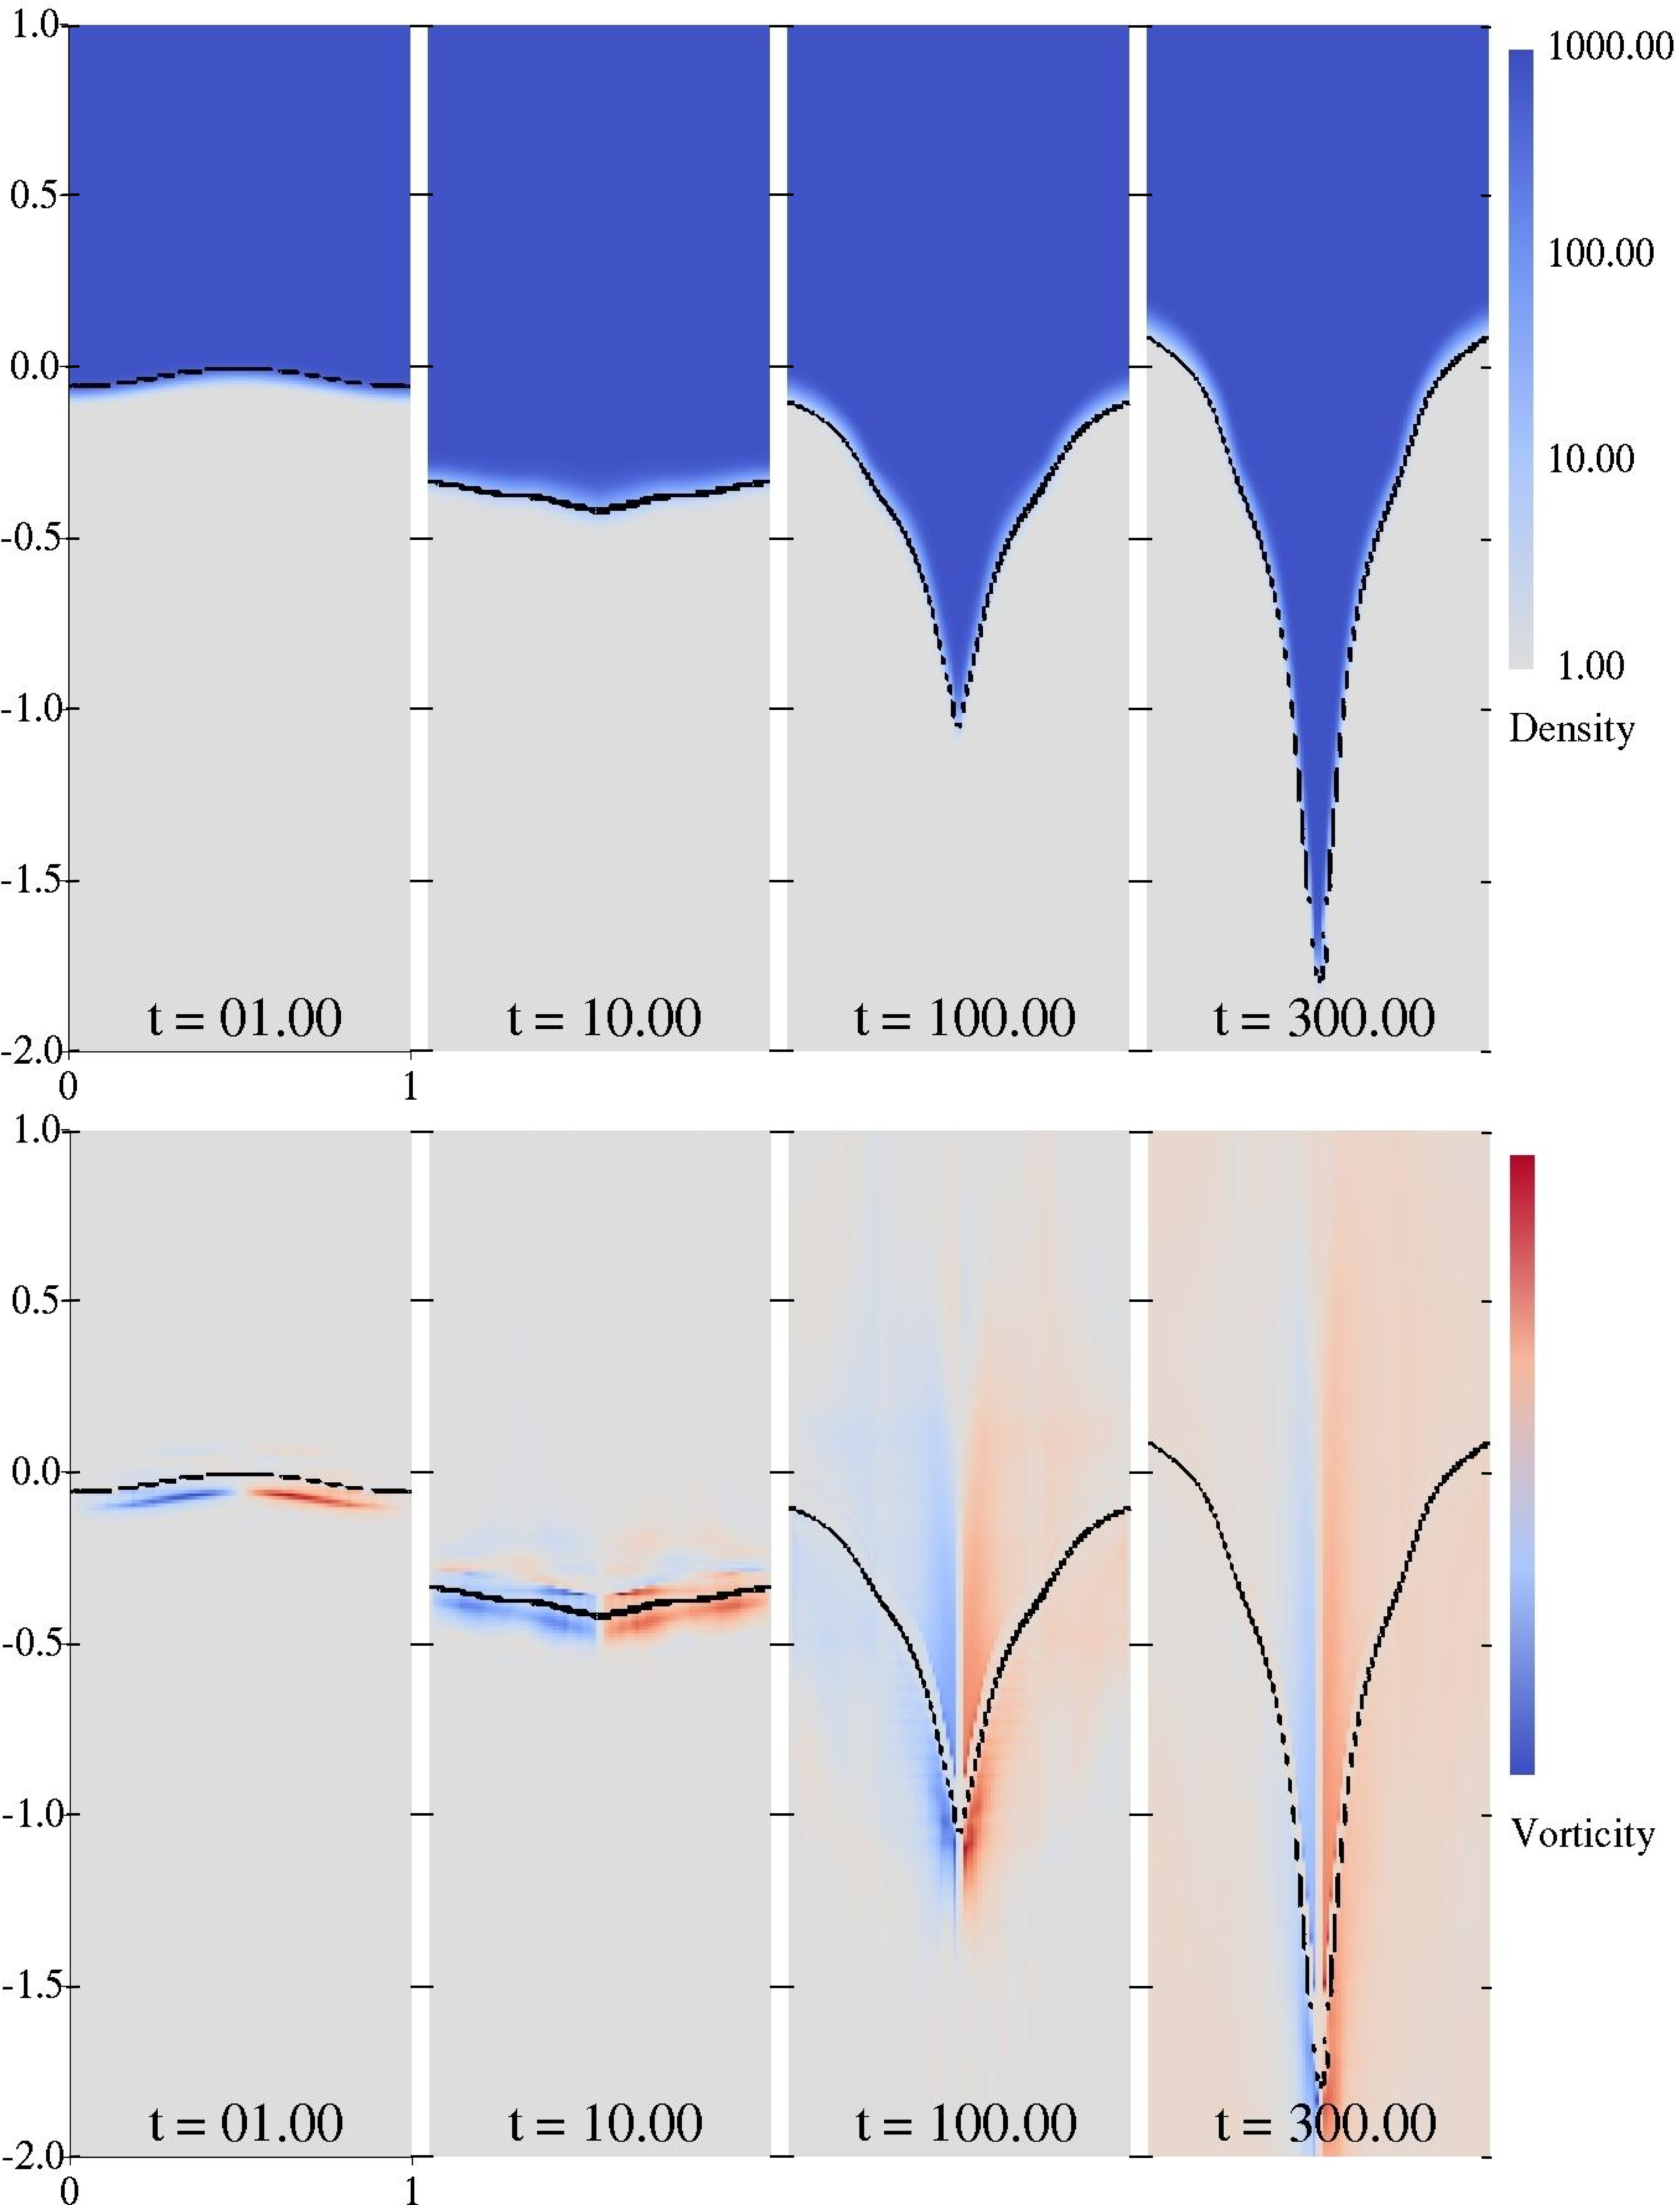
\includegraphics[width=0.9\textwidth]{./figs/lung_figs/snapshots_t1}
\caption[The evolution of the acoustically perturbed interface and vorticity field]{Surface plots of density (Top) and vorticity (Bottom)
  throughout the evolution of the interface for the $10$ MPa
  trapezoidal wave case. Areas of high density (i.e., water) are
indicated in dark blue. Areas of low density (i.e., air) are indicated
in white.  Positive (counterclockwise) vorticity is indicated in red,
and negative (clockwise) vorticity can be seen in blue.}
  \label{fig:interface_snapshots}
\end{figure}
%
\begin{figure}[h] 
  \centering
  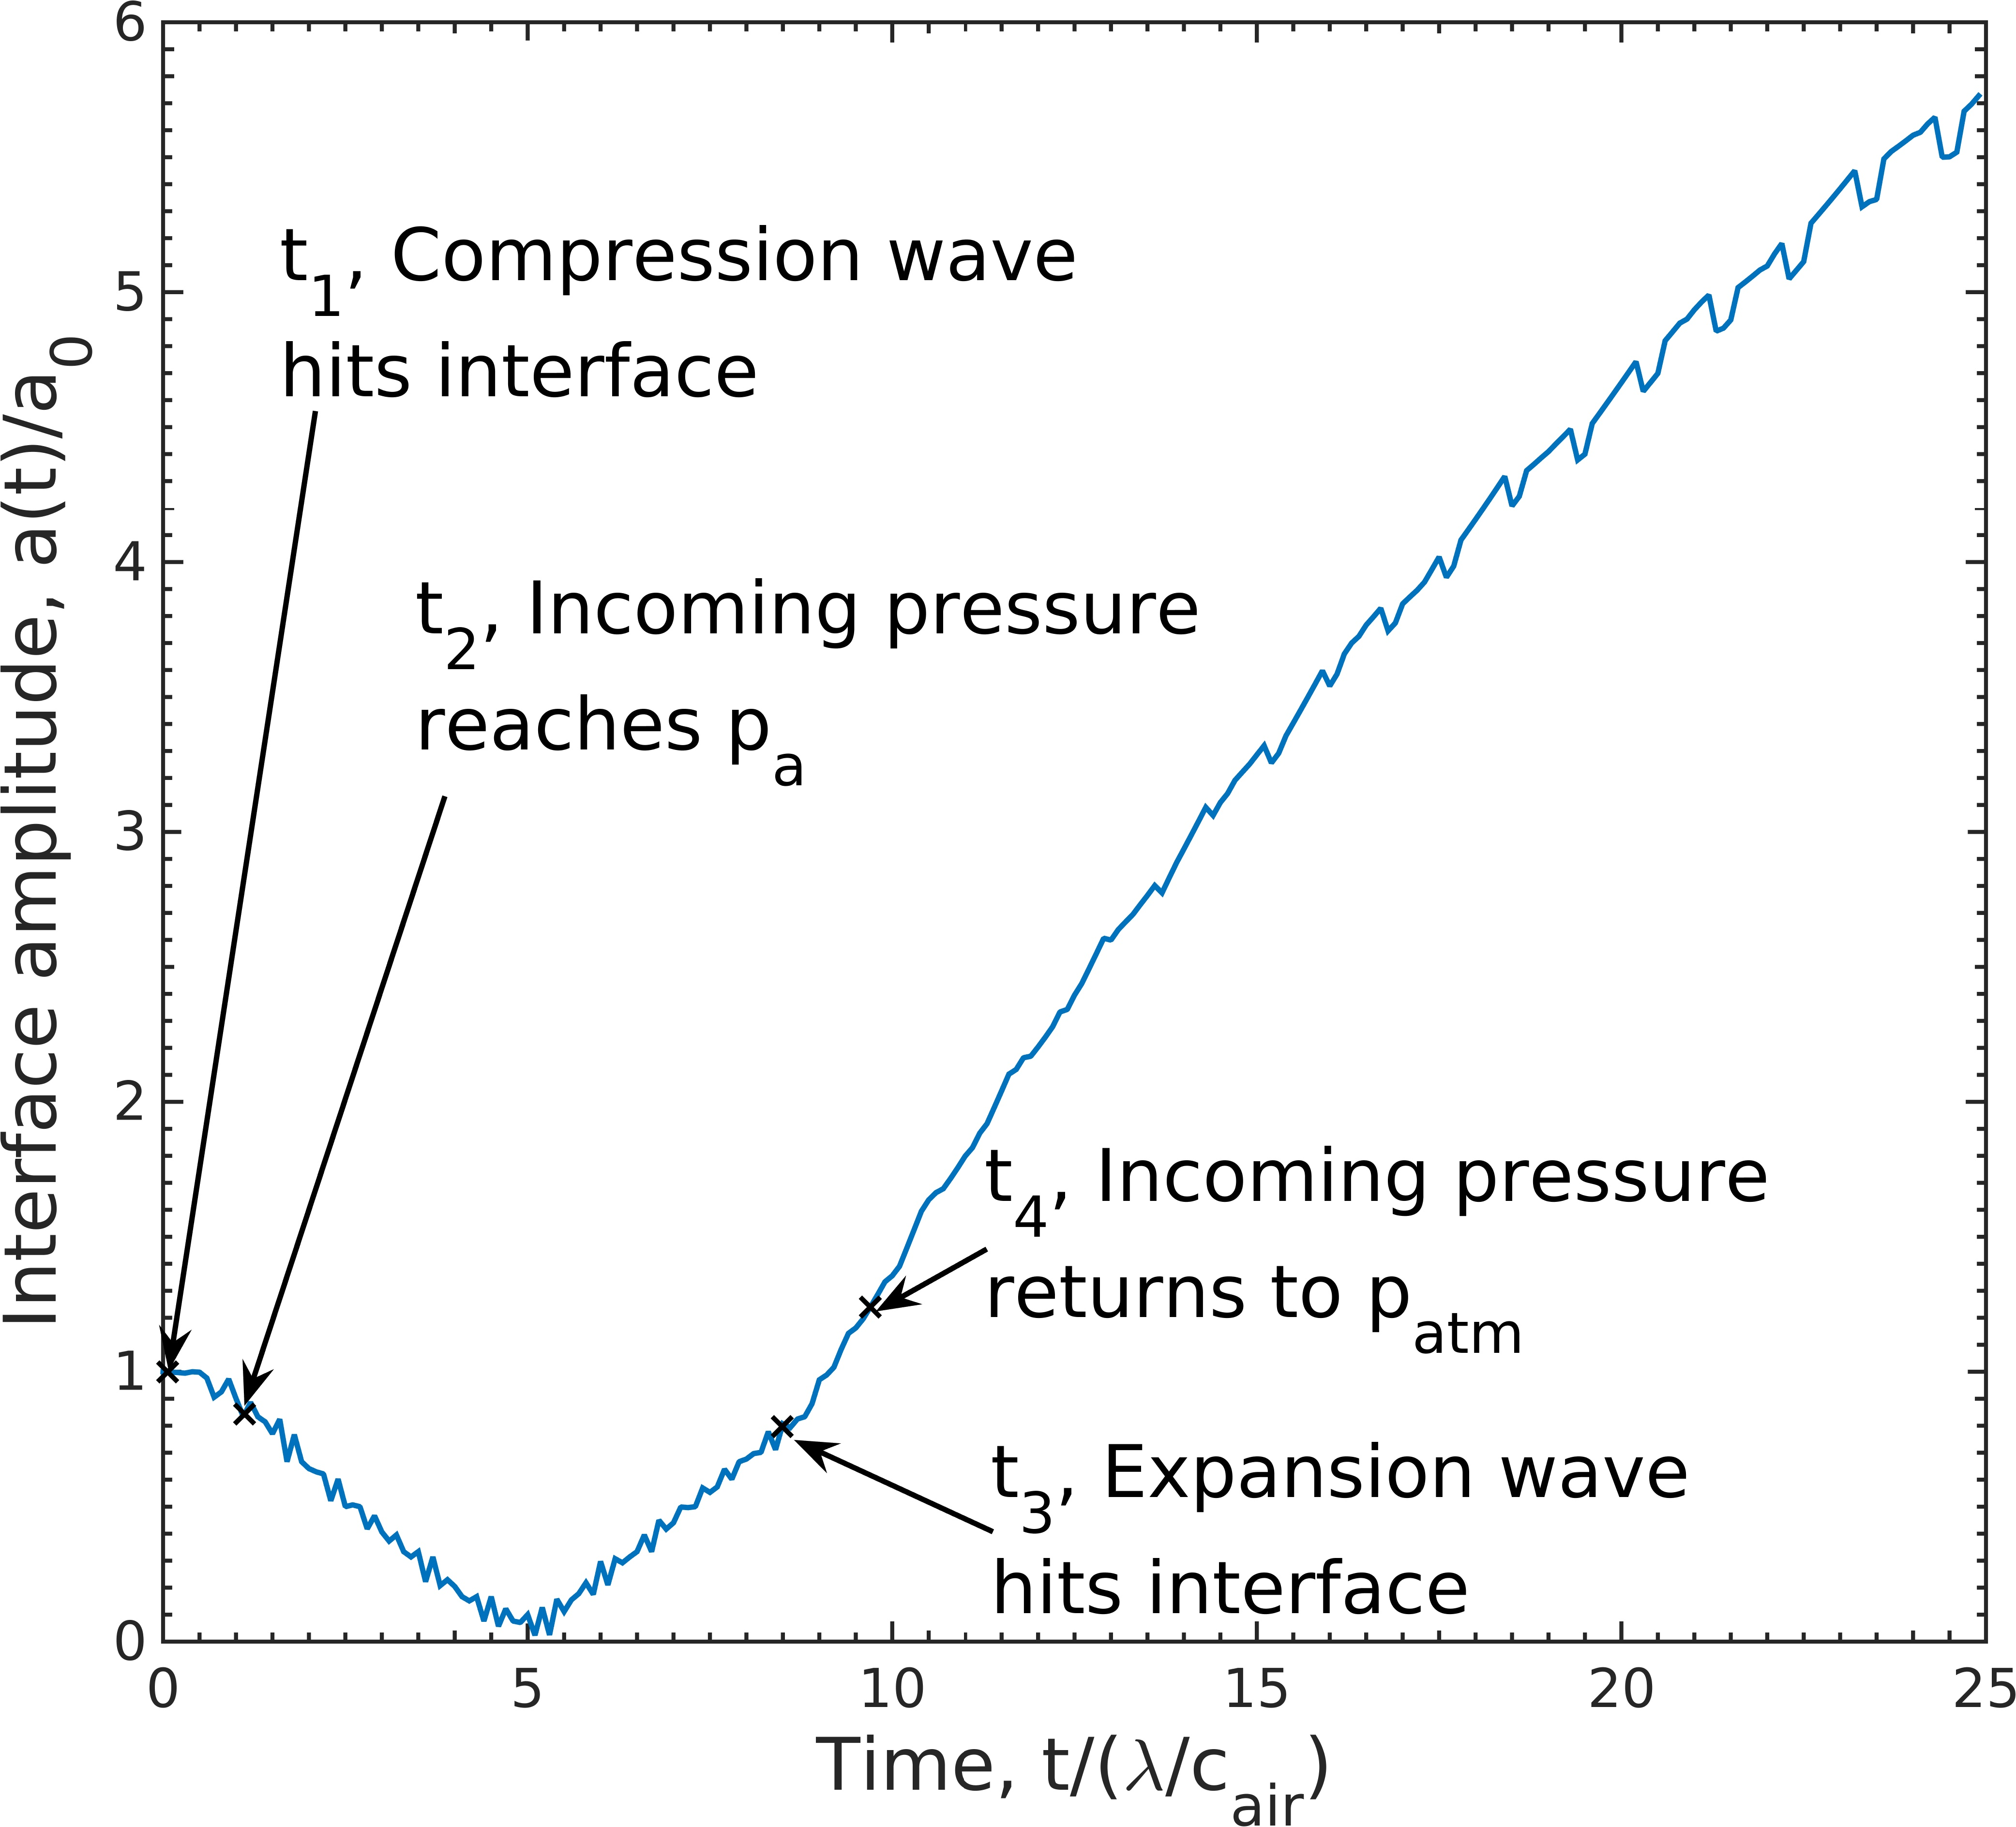
\includegraphics[width=0.48\textwidth]{./figs/lung_figs/trapz10_intf_schematic}
  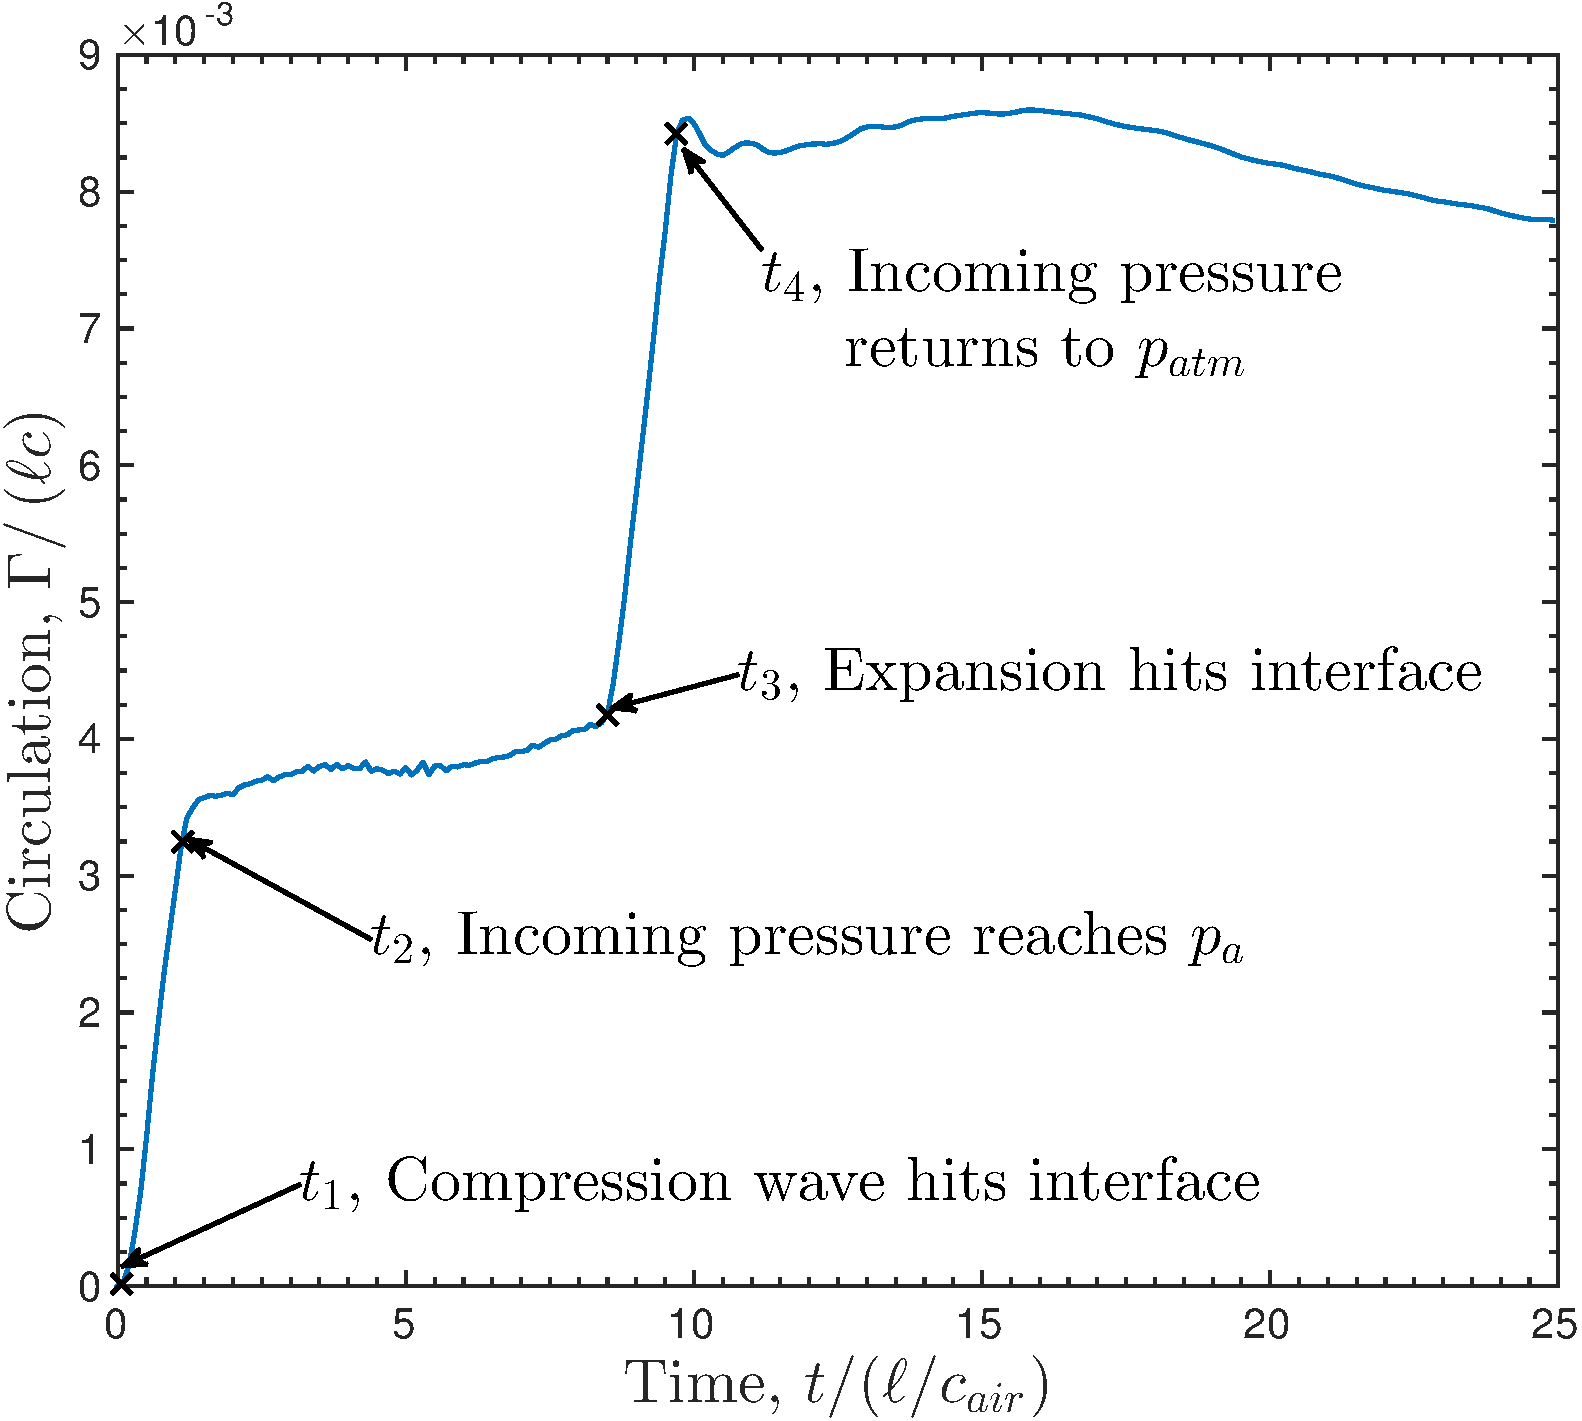
\includegraphics[width=0.48\textwidth]{./figs/lung_figs/trapz10_circ_schematic}
  \caption[The interface amplitude and circulation histories for the $10$ MPa trapezoidal wave]{The interface amplitude (left) and circulation (right)
    histories corresponding to the $10$ MPa trapezoidal waves are
    shown for $t\leq25$. Indicated times, $t_{1-4}$, are the times at
    which different stages of the incoming trapezoidal pressure wave
    shown in Figure \ref{fig:p0} first encounter the interface.}
  \label{fig:trapz10_circ_interface}
\end{figure}

\subsubsection{Dependence on acoustic wave amplitude}%
\label{subsubsec:usbe_lung_amplitude_dependence}%
To investigate the dependence of the dynamics on the trapezoidal wave
amplitude, we compare results for $p_a=1$, $5$, and $10$ MPa while
keeping the initial lengths of the wave $L$ and the rise and fall
$\Delta L_a$ constant such that $p_a$ scales linearly with the
acoustic pressure gradient. Figure
\ref{fig:trapz_circ_interface_early}, illustrates the interface
amplitude and $p_a$-normalized circulation histories for $t\leq25$,
during and shortly after the wave-interface interaction. Black
$\bs{\times}$s along the curves indicate $t_{1-4}$, described
previously in Subsection \label{subsec:Qualitative}. During the
interaction between the interface and the compression wave, the rate
at which the perturbation amplitude decreases is greater for higher
amplitude waves. The circulation deposited during this period scales
linearly with $p_a$ as is consistent with baroclinically-generated
circulation based on our analysis. For the $10$ MPa wave, the phase of
the interface inverts at, before the expansion hits, causing
circulation deposited by the expansion to have the same sign as that
deposited by the compression. For the $1$ and $5$ MPa waves interface
phase inversion occurs after the expansion and consequently deposits
circulation opposite that of the compression wave.

Figure \ref{fig:trapz_circ_interface_loglog} shows the interface
amplitude and circulation histories for $5$ and $10$ MPa trapezoidal
wave cases for $0 \leq t\leq 1000$. The perturbation amplitude history
is plotted on logarithmically-scaled axes. For both waves, the slope
of the perturbation amplitude is approximately $0.60$ long after the
waves have left the interface. This is slightly higher than the 0.5
slope predicted by scaling law \eqref{eq:intf_circ_scaling}. The
results for the $1$ MPa trapezoidal wave were not included because
interface evolved too slowly to obtain useful data given the
computational resources available.
%
\begin{figure}[h] 
  \centering
  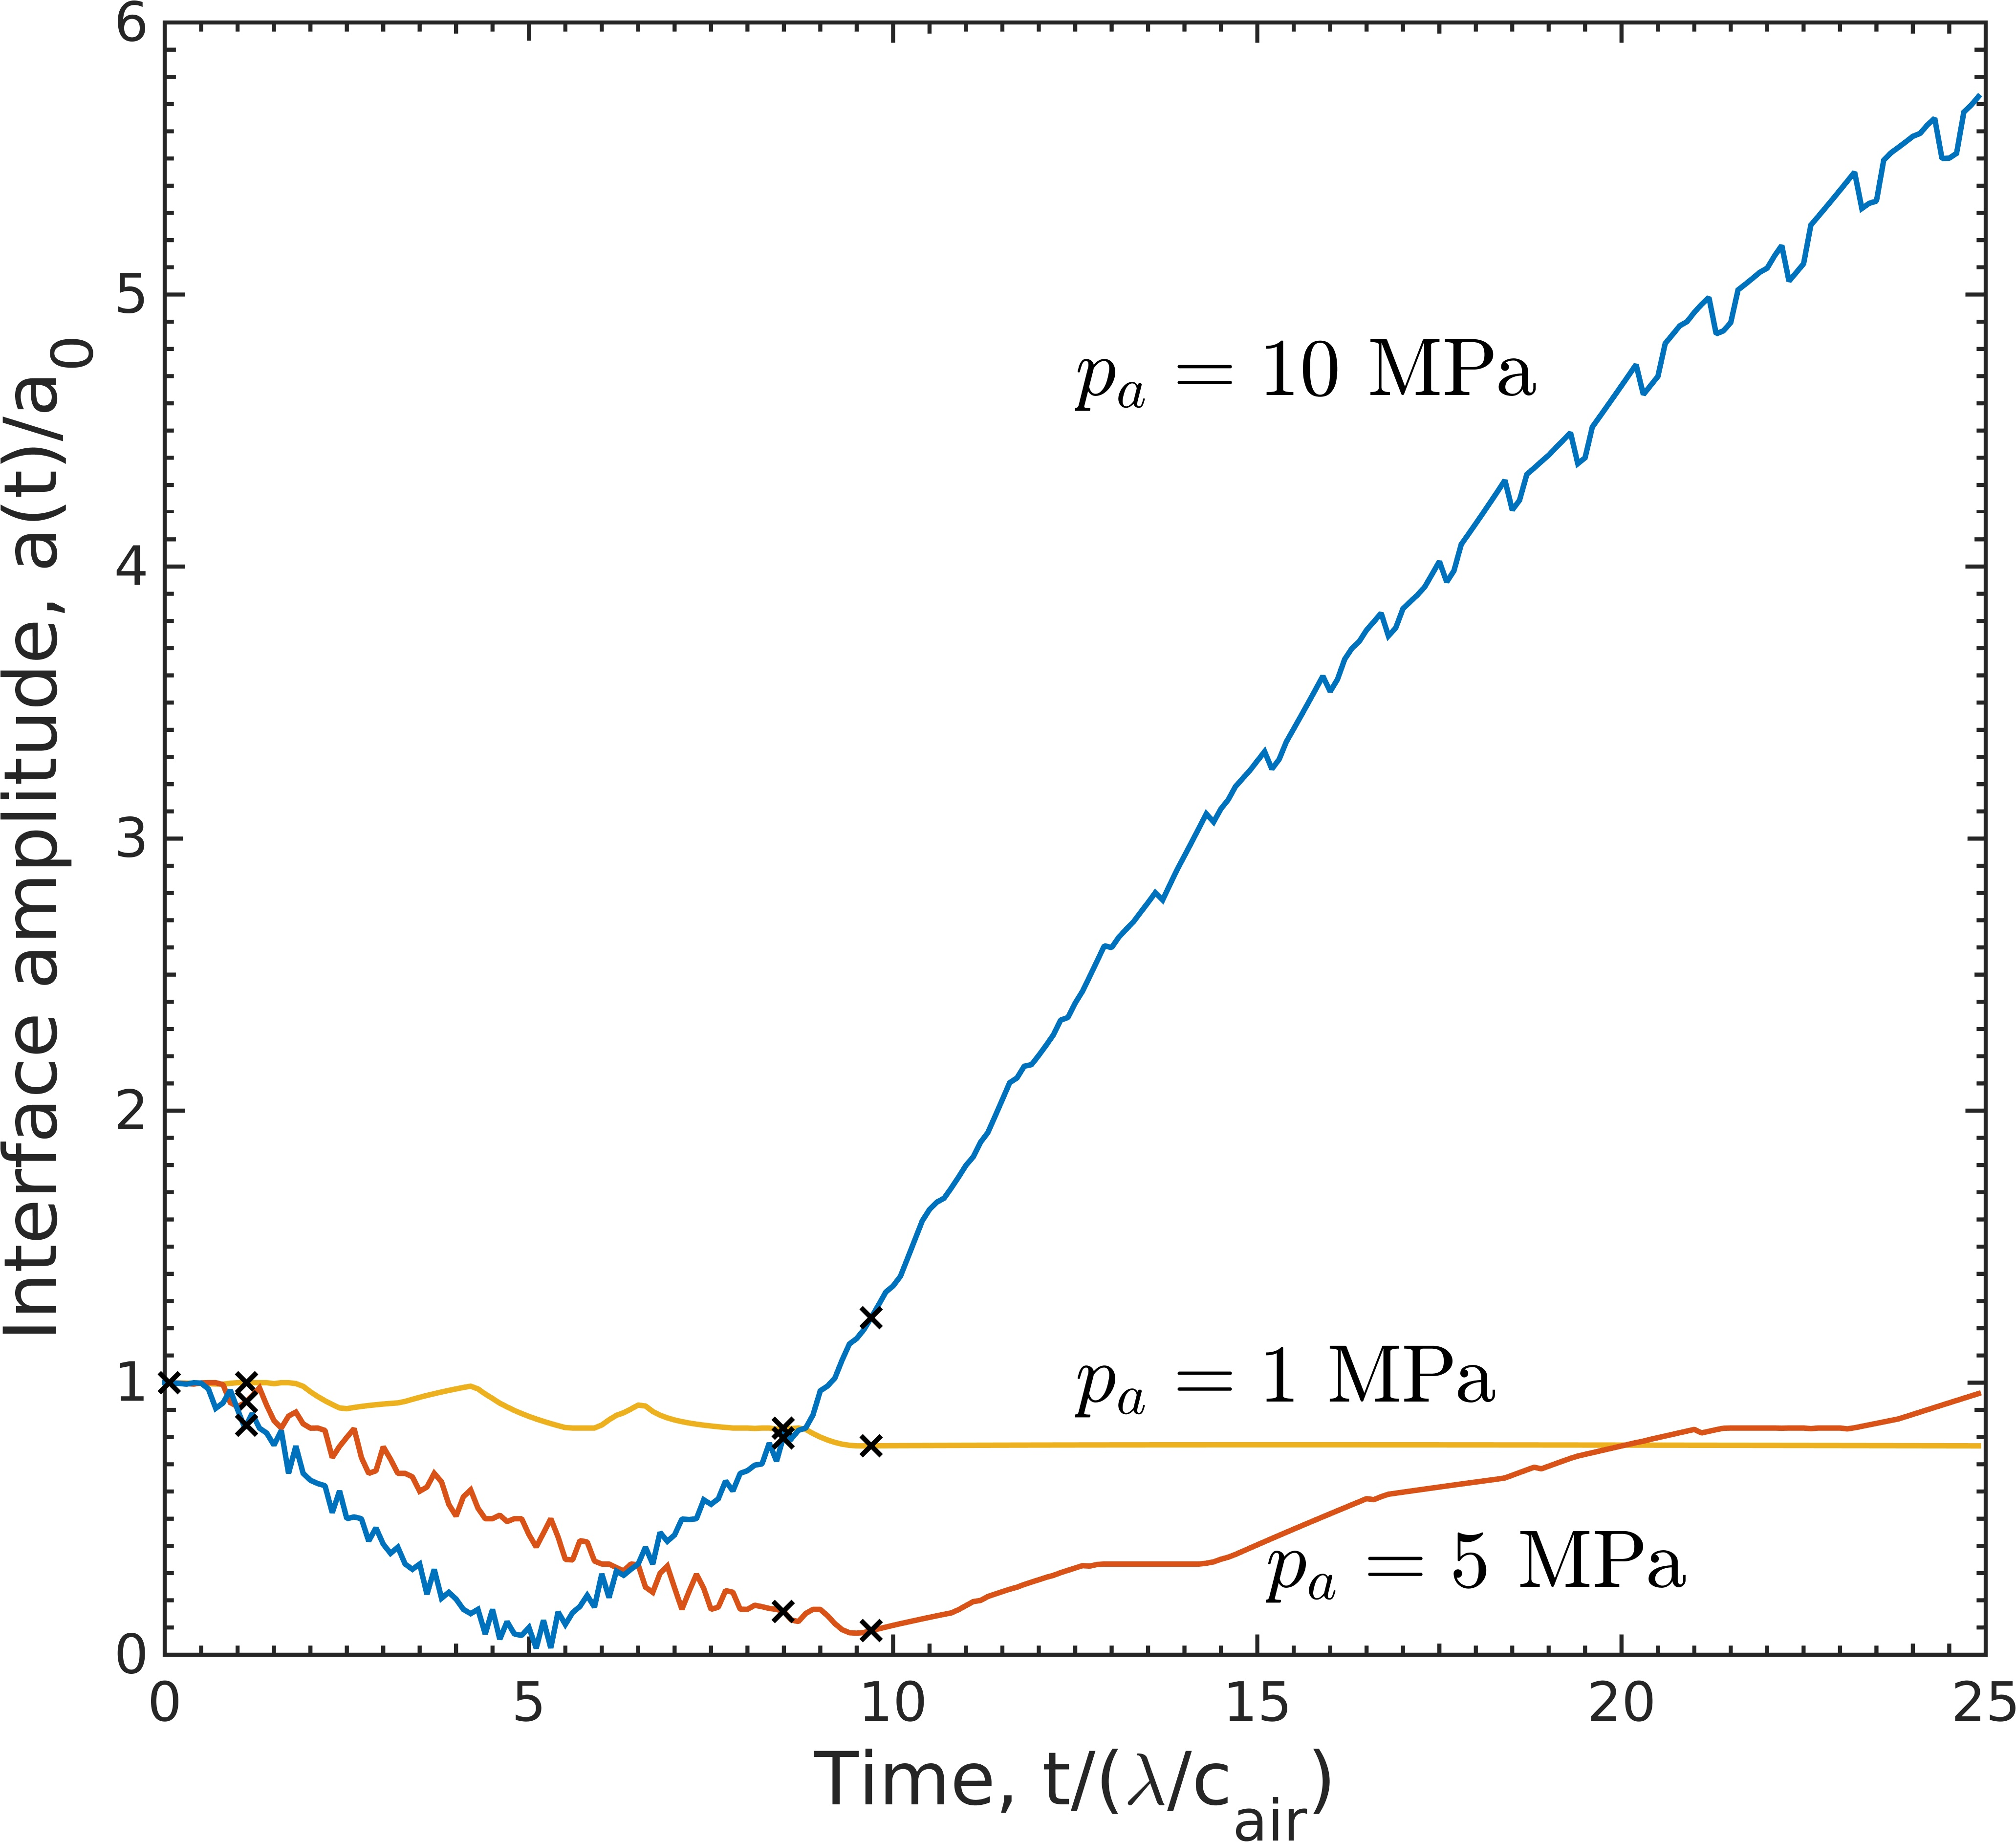
\includegraphics[width=0.48\textwidth]{./figs/lung_figs/interface_multi-amp_norm}
  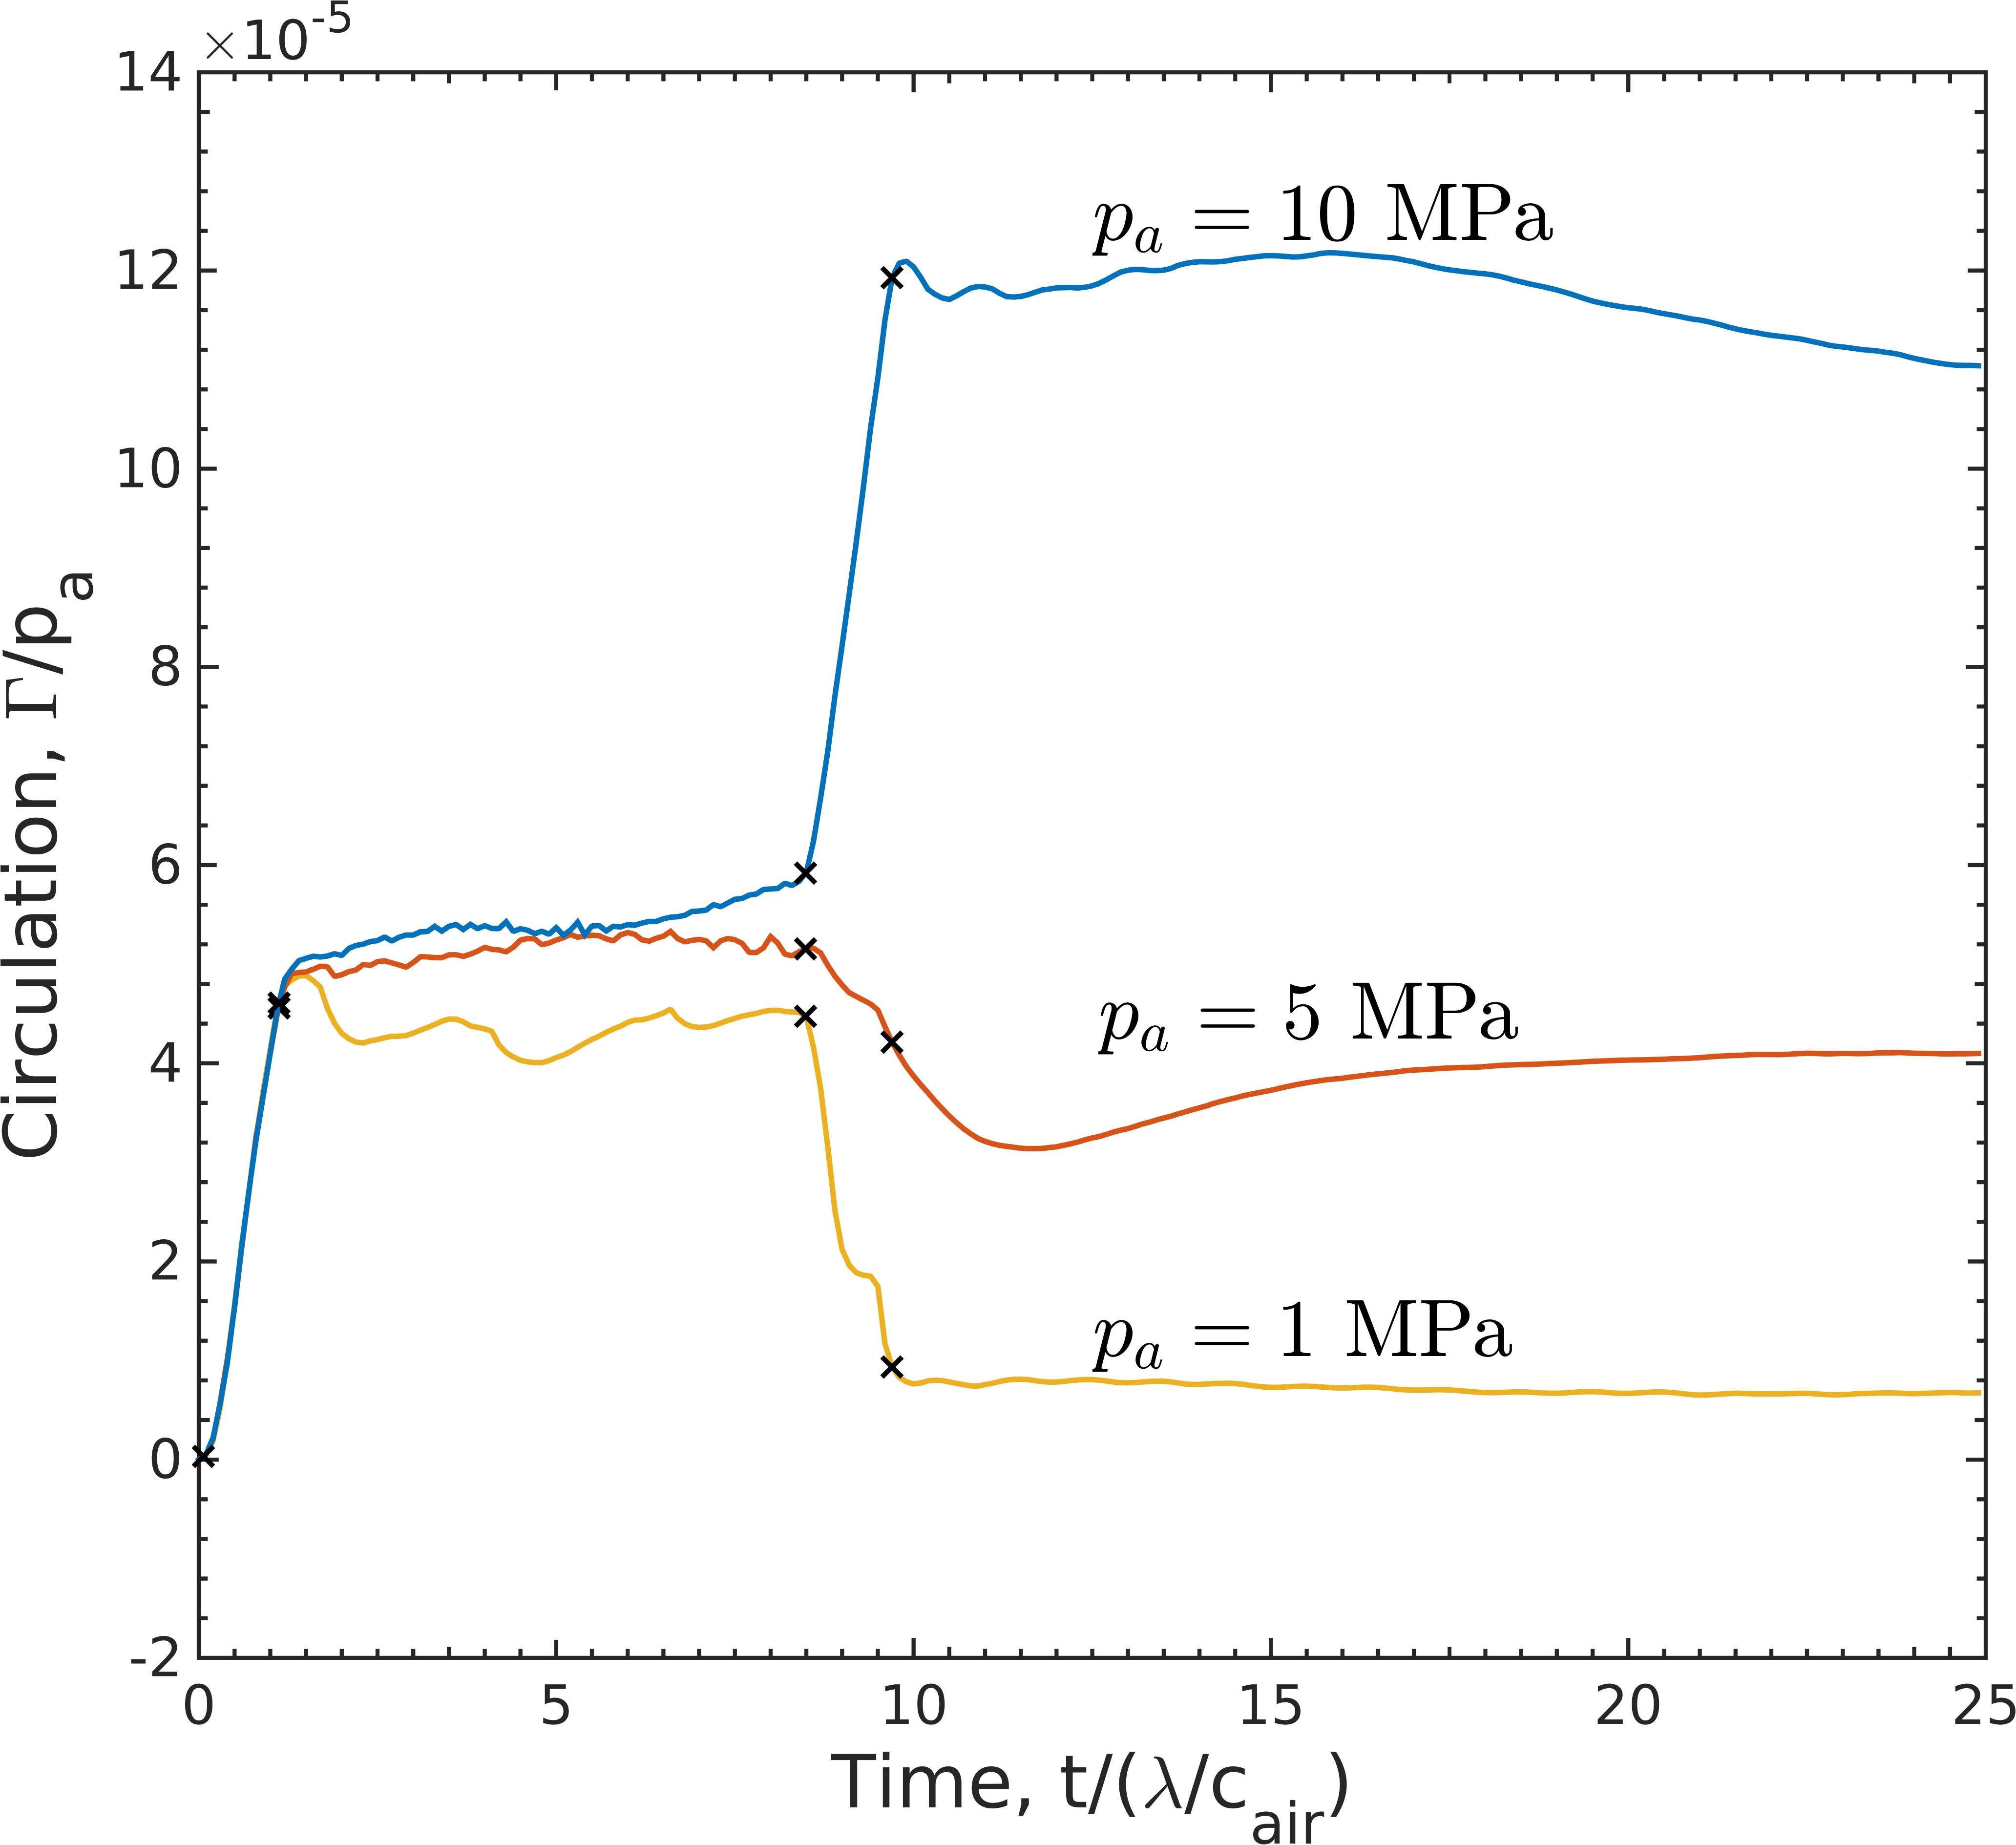
\includegraphics[width=0.48\textwidth]{./figs/lung_figs/circulation_multi-amp_norm}
  \caption[The interface and circulation dependence on wave amplitude at early time]{The interface amplitude (left) and circulation (right)
    histories corresponding to the $1$(yellow), $5$(orange), and
    $10$(blue) MPa trapezoidal waves are shown for $t\leq 25$. The
    circulation history is normalized by the acoustic amplitude of the
    incoming wave to illustrate that circulation deposition by the
    compression wave scales linearly with $p_a$.}
  \label{fig:trapz_circ_interface_early}
\end{figure}
%
\begin{figure}[h] 
  \centering
  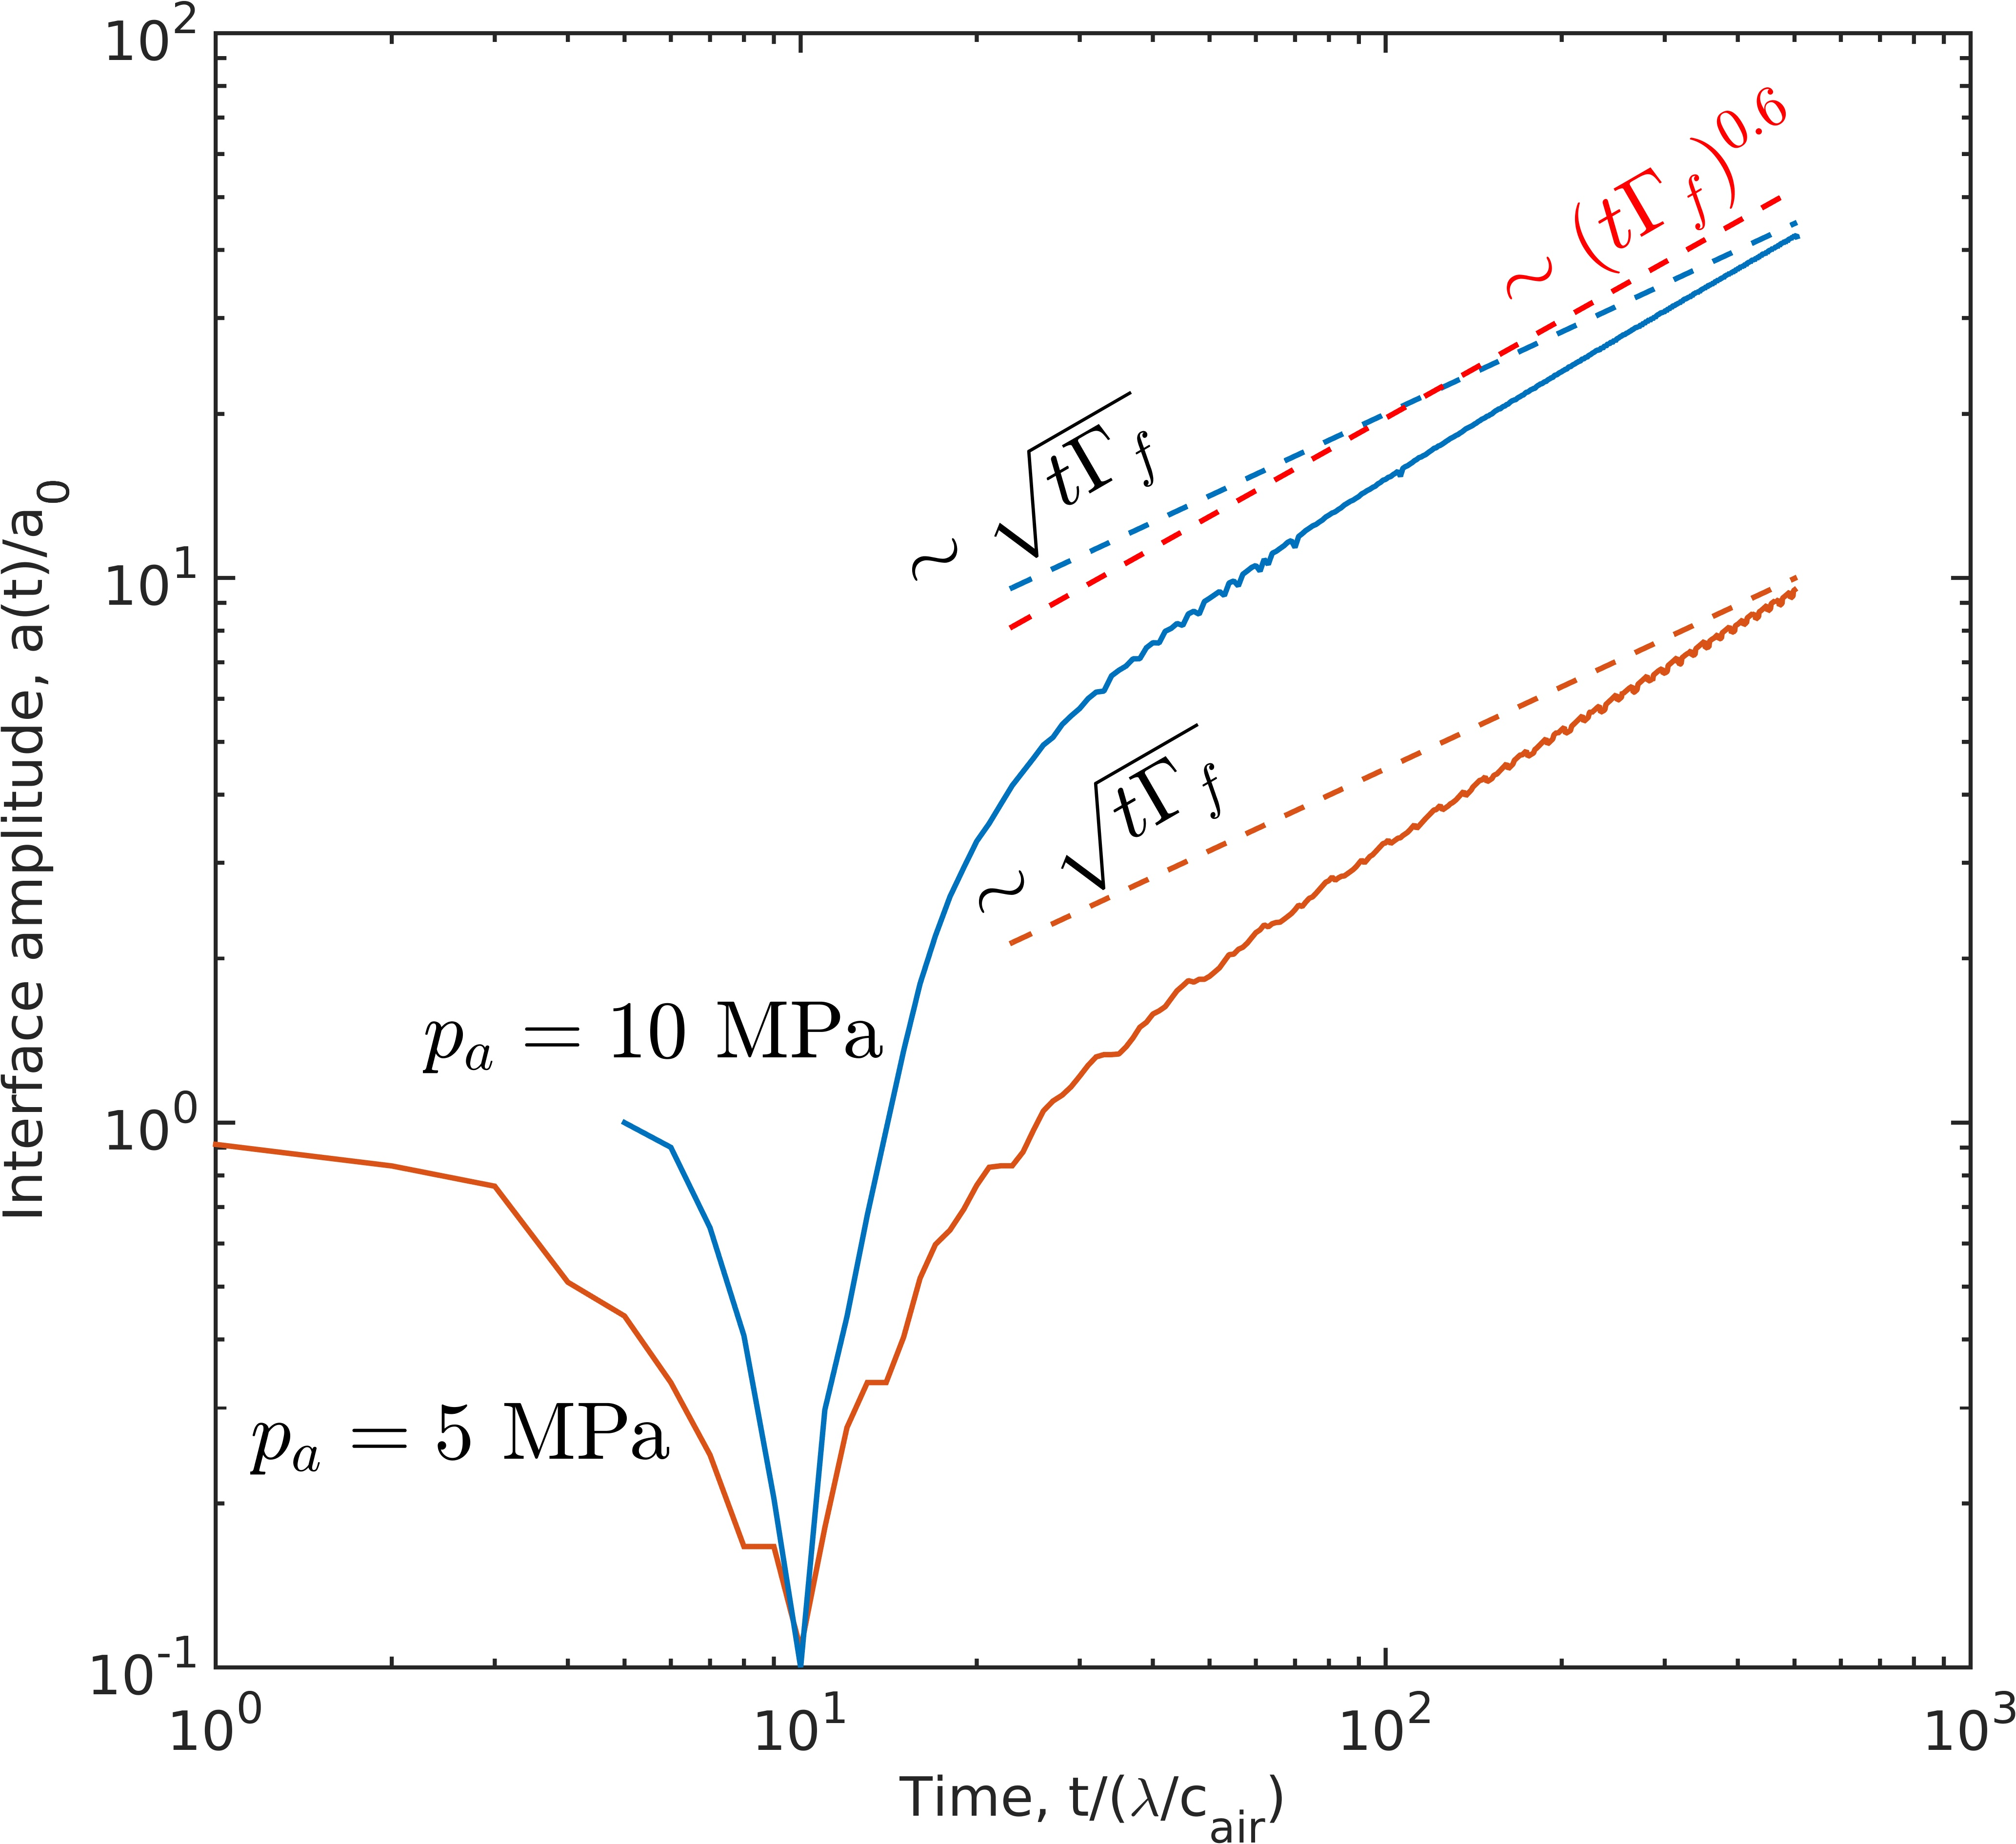
\includegraphics[width=0.48\textwidth]{./figs/lung_figs/interface_multi-amp_loglog_roe_extra}
  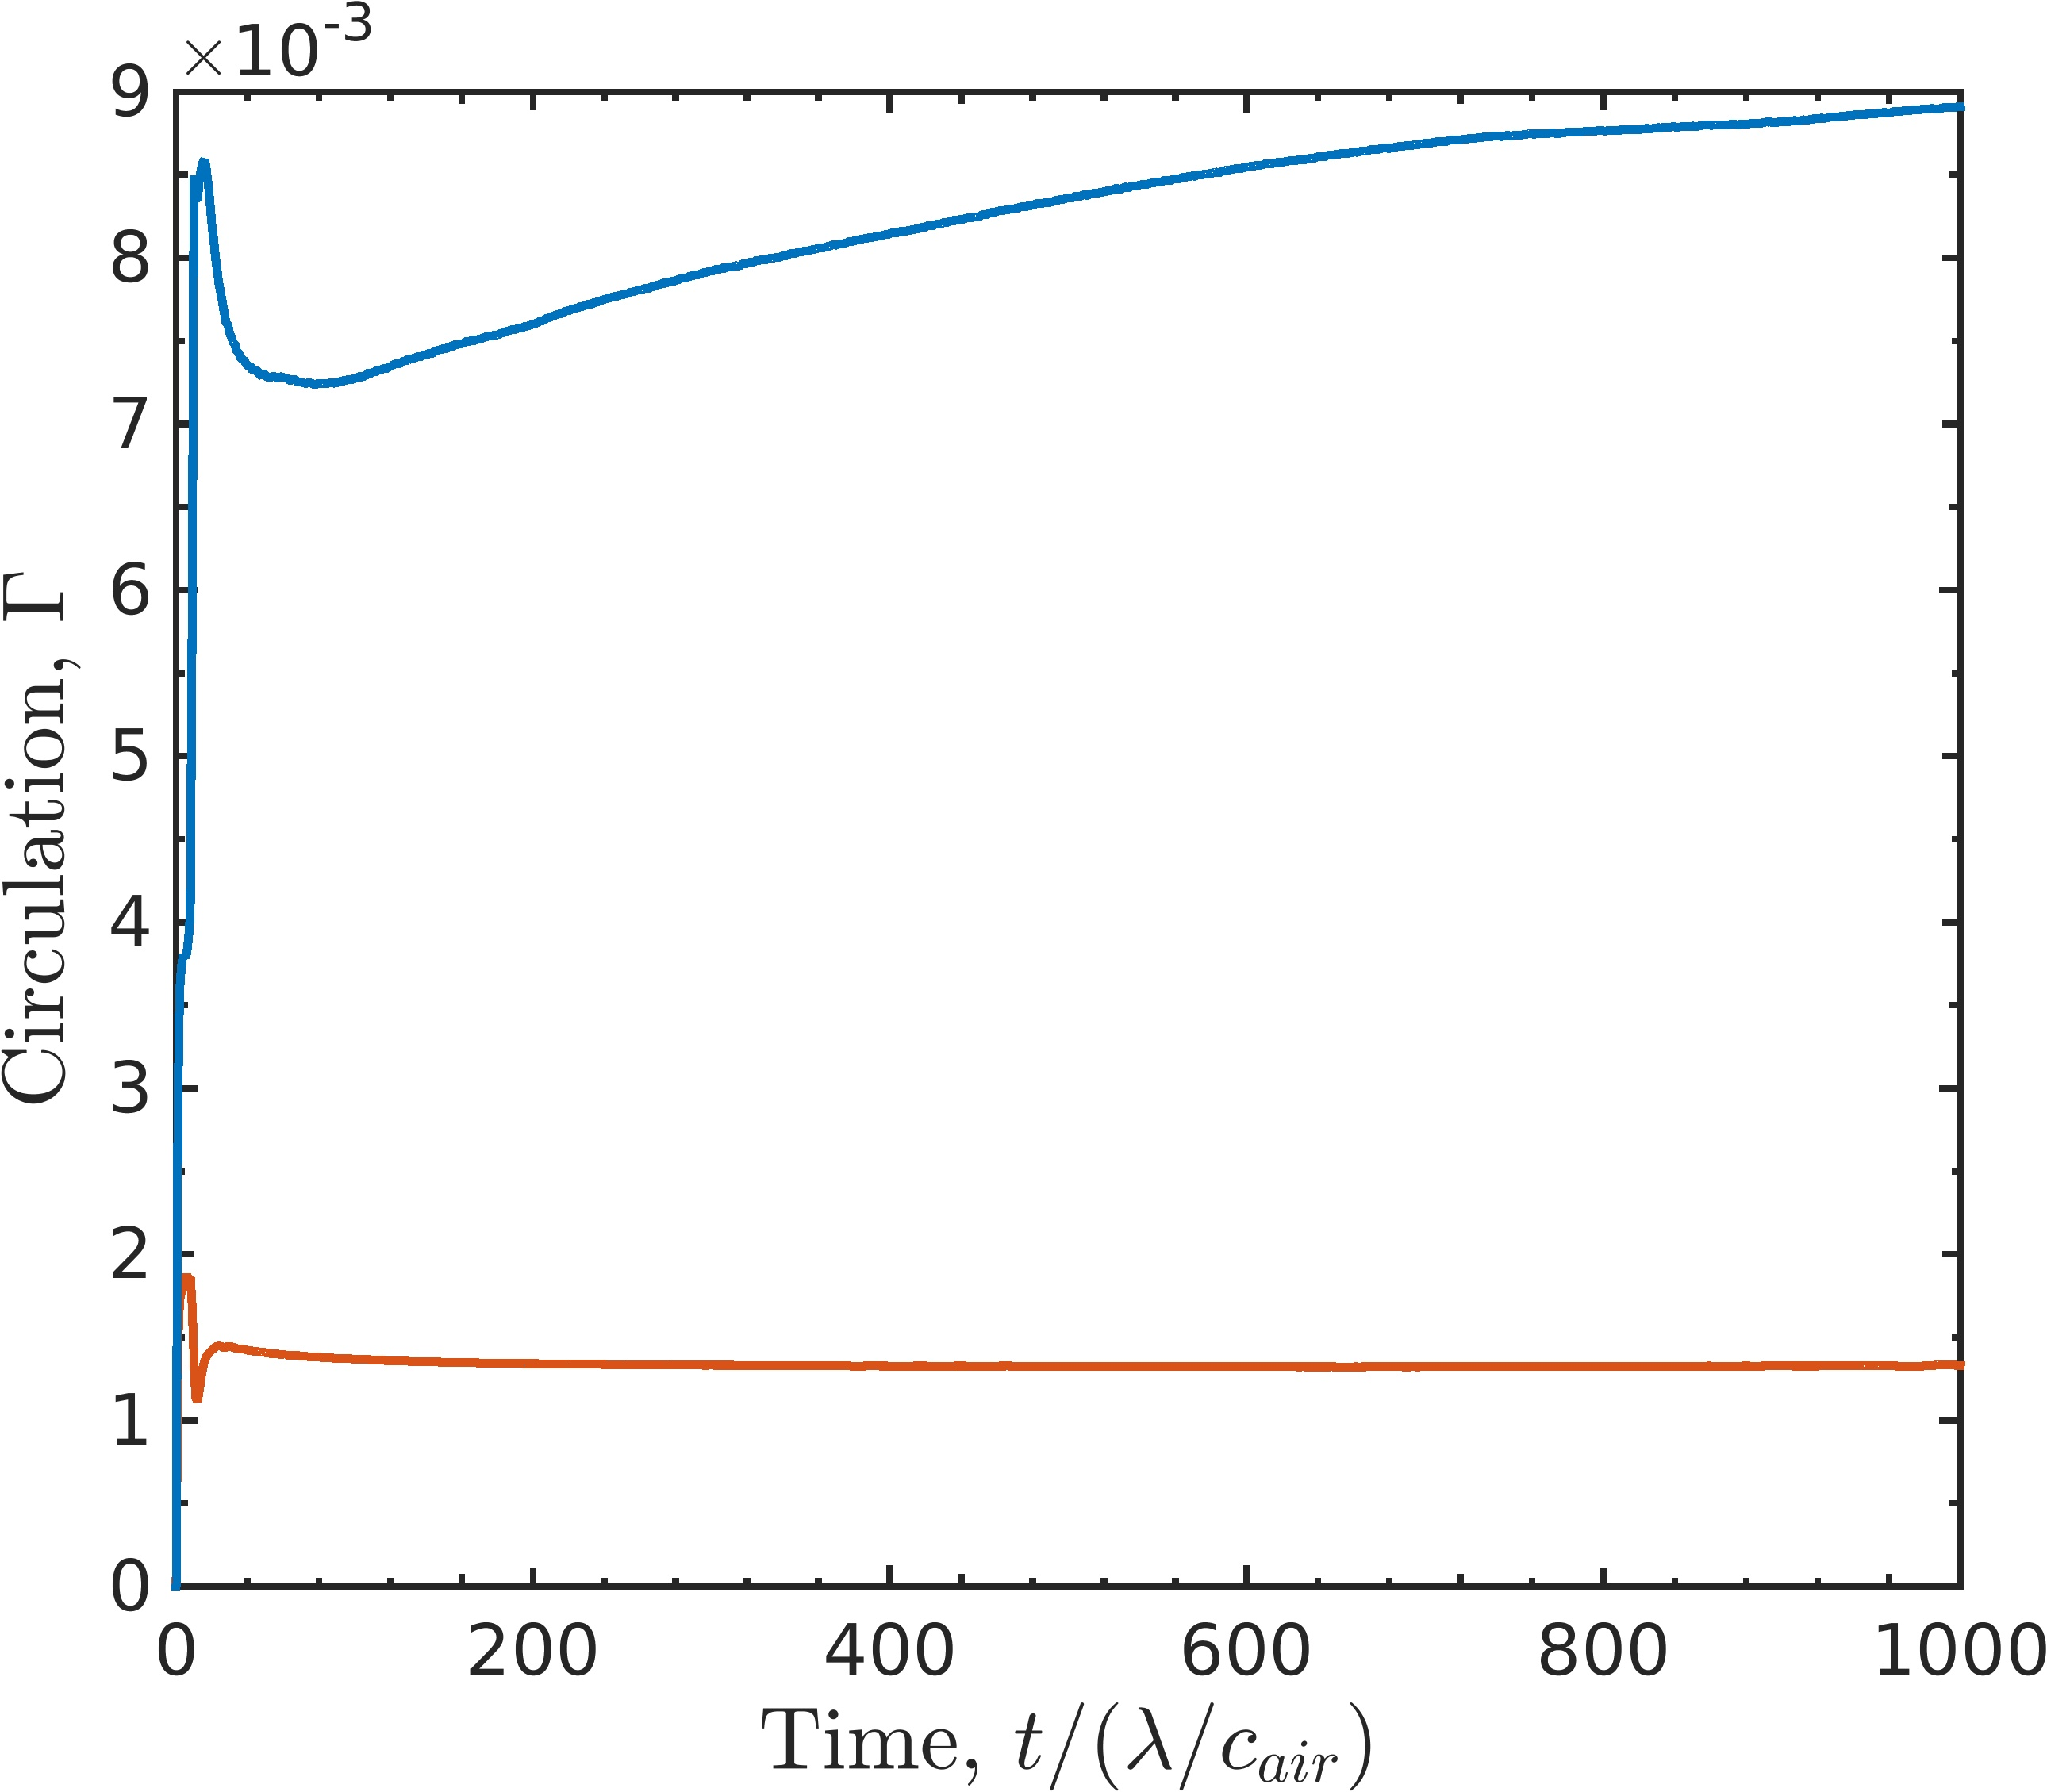
\includegraphics[width=0.48\textwidth]{./figs/lung_figs/circulation_multi-amp2_roe_fixed}
  \caption[The interface and circulation dependence on wave amplitude
  at long time]{The interface amplitude (left) and circulation (right)
    histories corresponding to the $5$(orange) and $10$(blue) MPa
    trapezoidal waves are shown for $t\leq 500$. To appropriately
    compare late time dynamics, time has been offset in the interface
    amplitude history such that the phase reversal appears to occur
    simultaneously in both simulations. Dashed lines of the same color
    are used to demonstrate the expected slope of pure circulation
    driven interface growth, based on Equation
    \eqref{eq:intf_circ_scaling}. The red dashed line shows the slope we
    appear to be approaching for the $10$ MPa wave case for the end time.}
  \label{fig:trapz_circ_interface_loglog}
\end{figure}
%
\subsubsection{Circulation and vorticity dynamics}
We observe that the wave deposits a sheet of vorticity along the
interface that moves with the interface in time. Figure
\ref{fig:interface_snapshots} shows a surface plot of vorticity in the
region of the domain around the interface for the $10$ Mpa trapezoidal
wave case, at $t=1.0$, during the middle of the interface-compression
wave interaction (Left). Not shown is the rest of the domain, where
vorticity was relatively insignificant. The vorticity is antisymmetric
across the $x=0.5$ center line. To analyze the physical mechanisms
generating the vorticity, we plot each term of the circulation
generation equation \eqref{eq:circulation_generation} during the
period around the compression wave-interface interaction. Near the end
of the interaction at $t=1.0$,
$\left(\partial \Gamma/\partial t\right)_{advective} =
-5.3\,\text{e}{-5}$; %
$\left(\partial \Gamma/\partial t\right)_{compressible} =
2.7\,\text{e}{-5}$; %
$\left(\partial \Gamma/\partial t\right)_{baroclinic} =
7.7\,\text{e}{-3}$; %
$\left(\partial \Gamma/\partial t\right)_{total} =
7.7\,\text{e}{-3}$. %
This result is quantitatively consistent with expected vorticity generation
based on our analysis \eqref{eq:vorticity_comparison}. Furthermore, it
supports our hypothesis that vorticity is primarily baroclinically
generated. 
%
\begin{figure}[h] 
  \centering
%  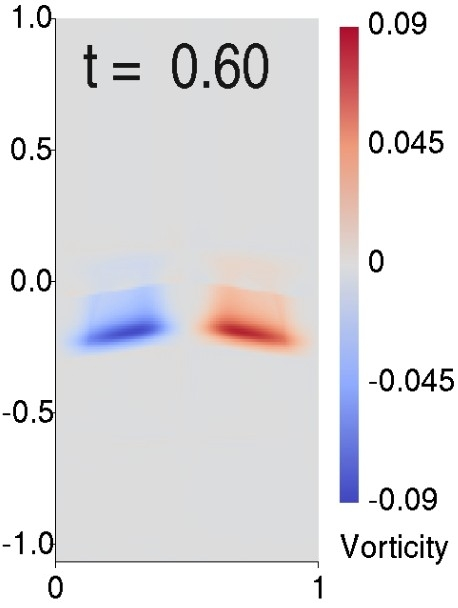
\includegraphics[width=0.35\textwidth]{./figs/lung_figs/vorticity2}
  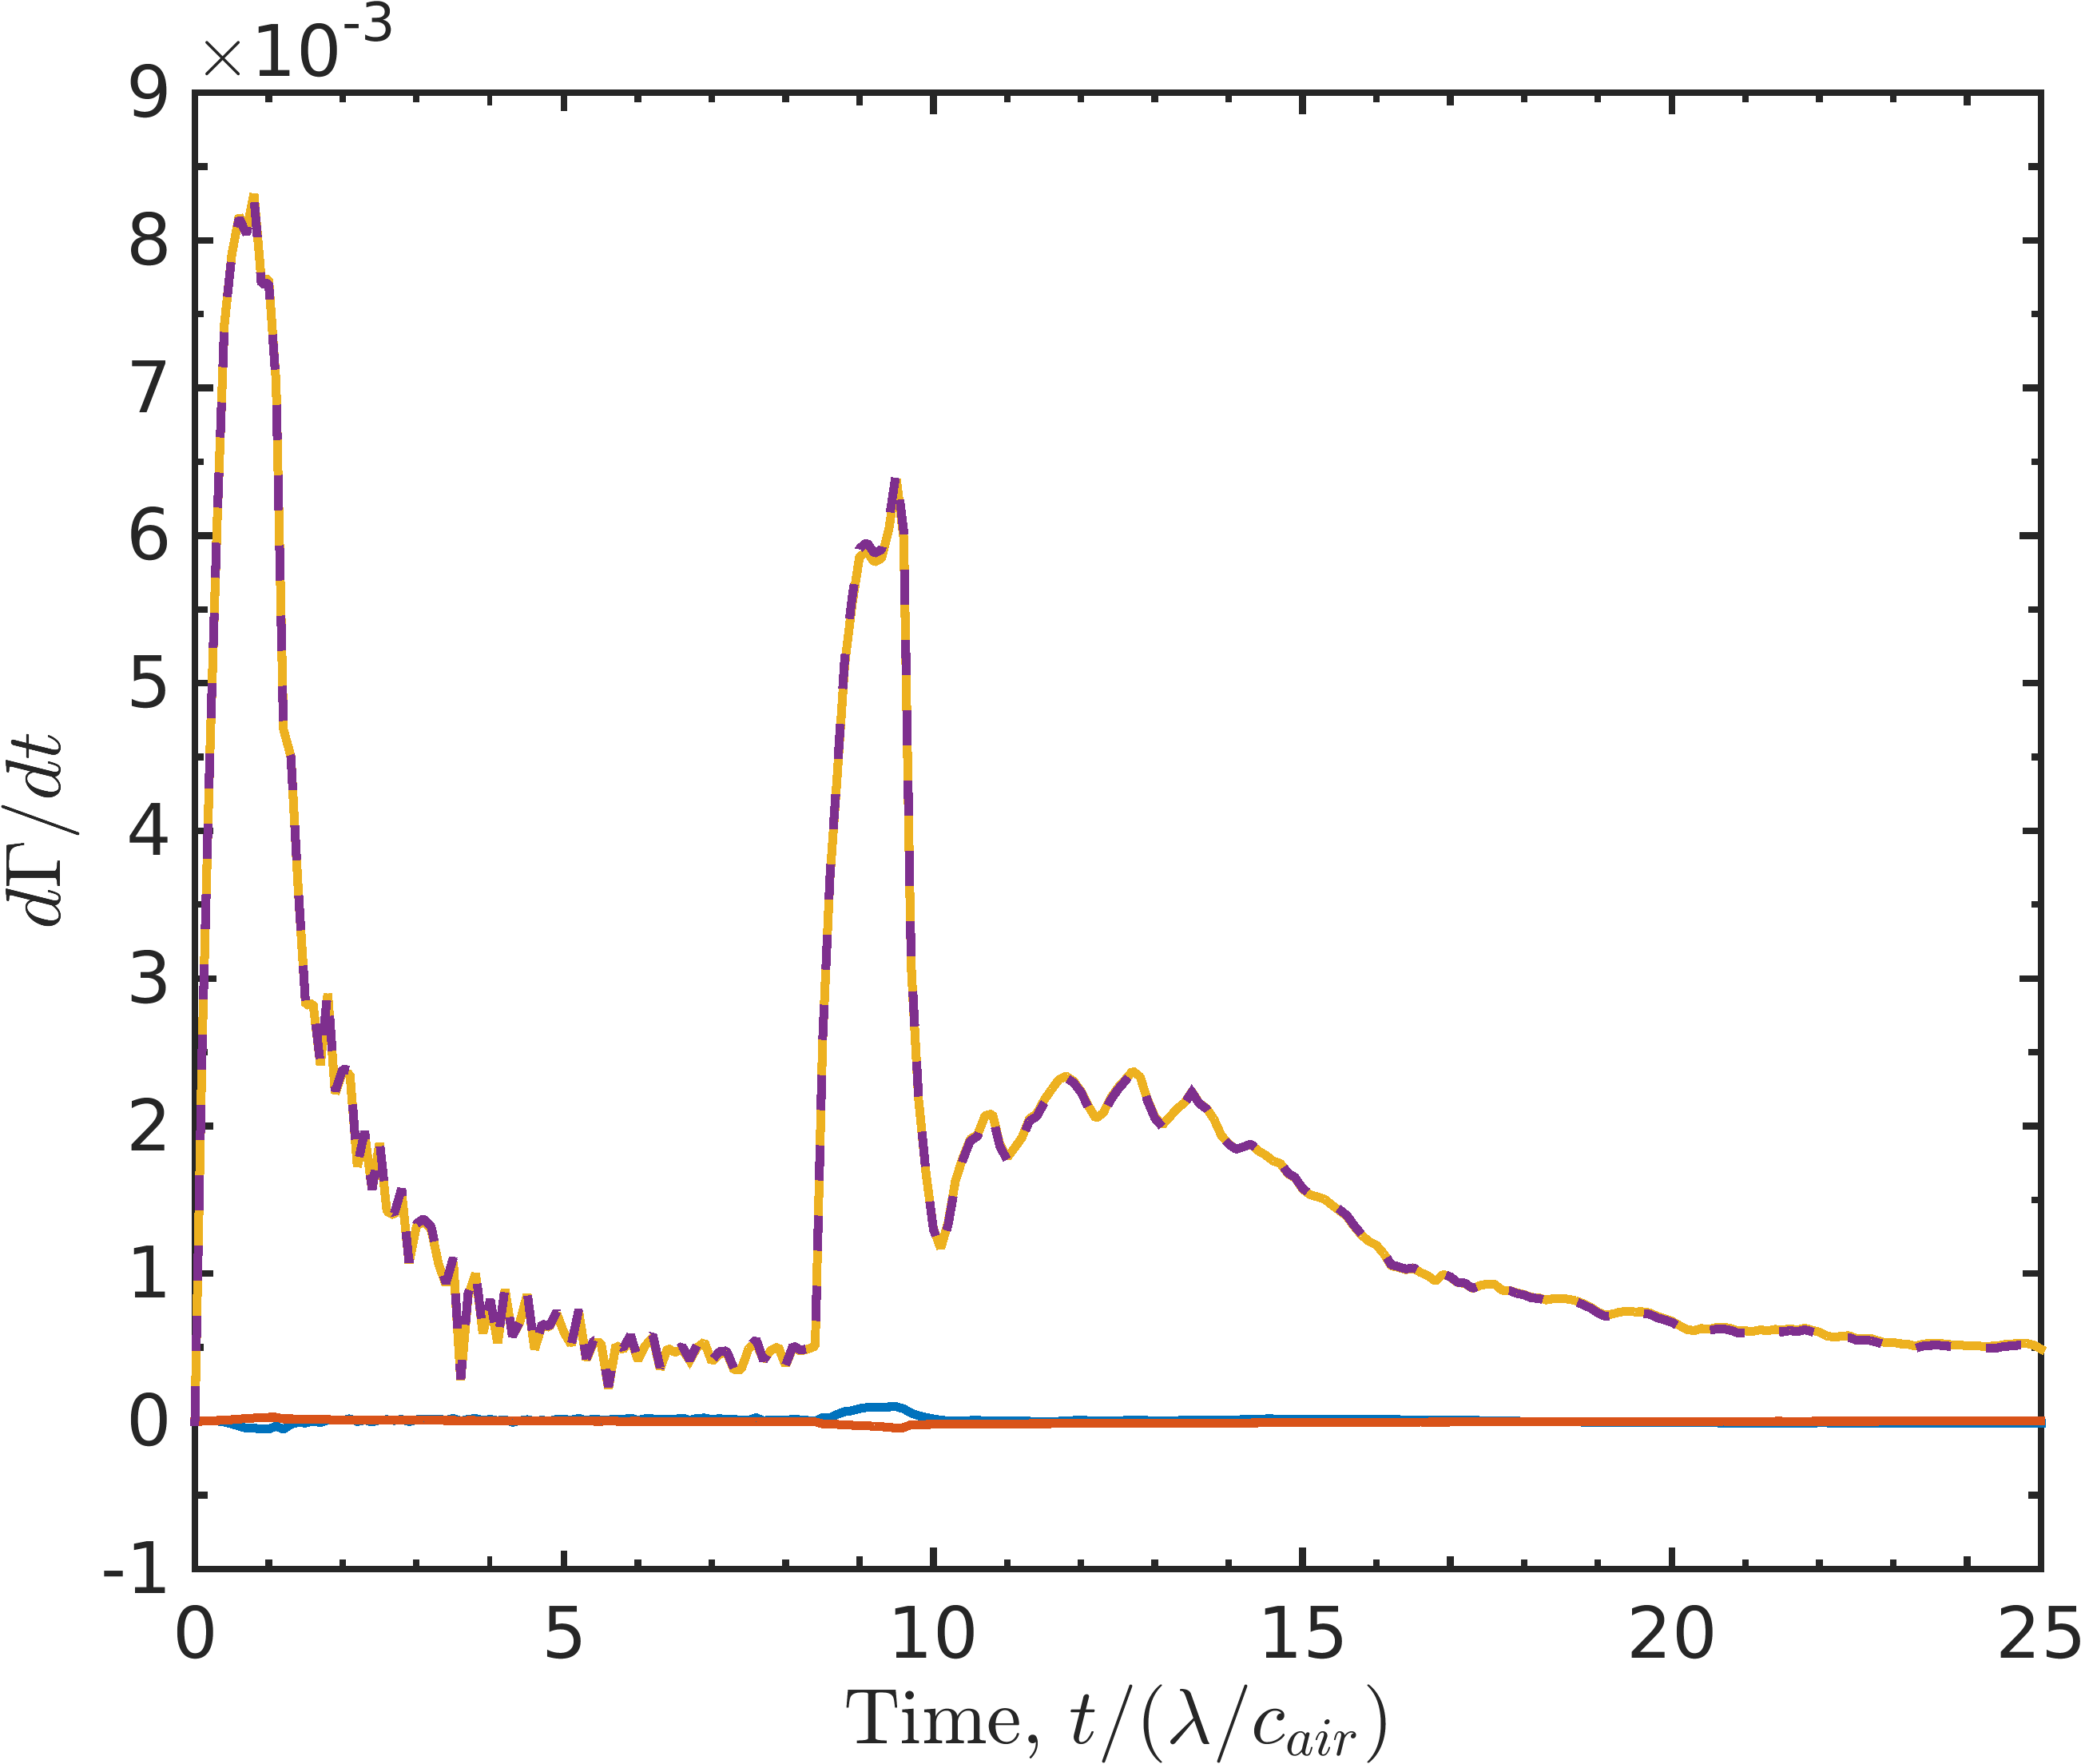
\includegraphics[width=0.48\textwidth]{./figs/lung_figs/ddtcirc_fixed}
  \caption[The individual contributions to circulation generation by physical mechanism]{Each term of the
    circulation generation equation \eqref{eq:circulation_generation} is plotted as a function of time:
    $\left(d\Gamma/dt\right)_{advective}$ (blue),
    $\left(d\Gamma/dt\right)_{compressible}$ (orange),
    $\left(d\Gamma/dt\right)_{baroclinic}$ (yellow),
    $\left(d\Gamma/dt\right)_{total}$ (purple, dashed).}
  \label{fig:trapz_ddt_circ}
\end{figure}
%
\subsubsection{Dependence on the length of the wave}%
To investigate the dependence of the dynamics on the length of the
trapezoidal wave $L$, and comparably the wave-interface interaction
time, we compare results for $p_a=10$ MPa waves of constant rise and
fall length $\Delta L_a$. This effectively changes the time the
interface has to evolve while experiencing the constant elevated
pressure portion of the wave between the compression and expansion.
Figure \ref{fig:trapz_circ_interface_multi-lag} shows the interface
amplitude and circulation histories corresponding to waves with
$L=45\lambda, 35\lambda ,30\lambda ,25\lambda ,15\lambda ,10\lambda$
for $0 \leq t\leq 25$.  For the three longest waves, $L \geq 30\lambda$,
the expansion encounters the interface after the perturbation reverses
phase. In these cases, the expansion deposits additional positive
circulation along the right half of the interface. For the shorter
waves, $L \leq 25\lambda$, the expansion encounters the interface before
the perturbation reverses phase and the net half-domain circulation is
decreased. Comparing cases in which the interface inverts phase before
the expansion occurs the larger $a(t)$ is at the time, the more
circulation is generated. The same is true when comparing cases in
which the phase inversion occurs after the interface inverts phase.
%
\begin{figure}[h] 
  \centering
  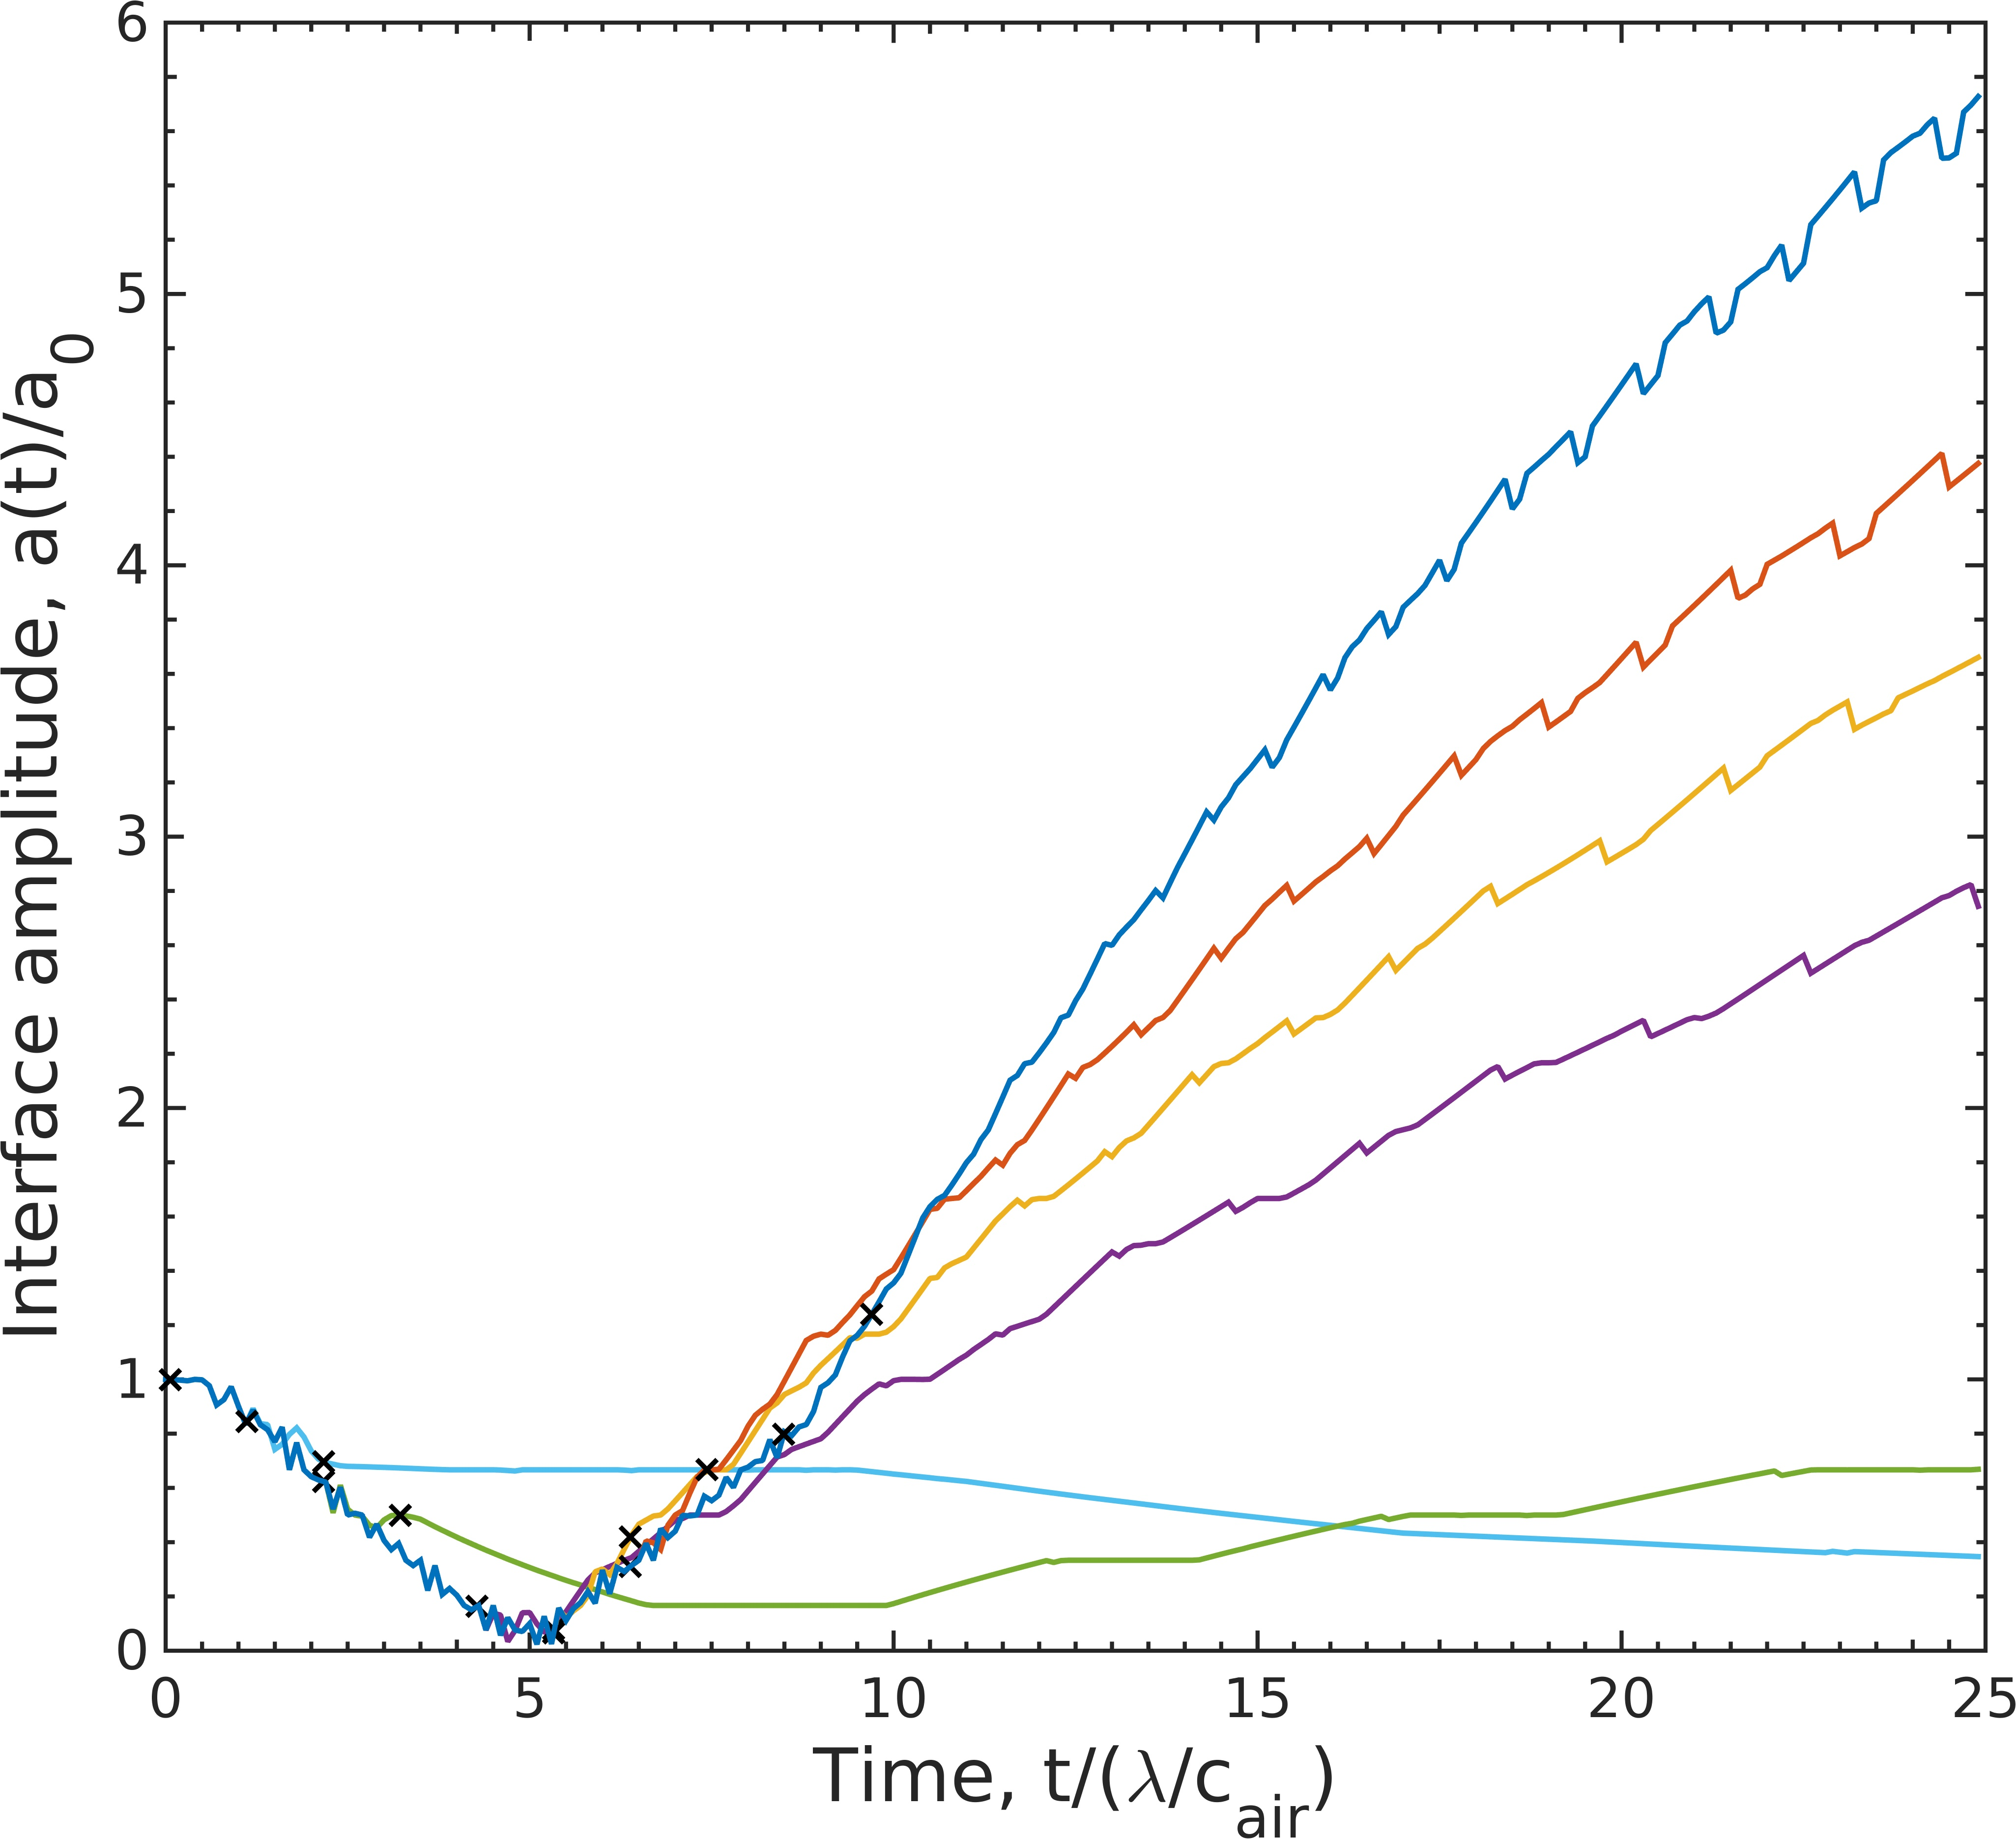
\includegraphics[width=0.48\textwidth]{./figs/lung_figs/interface_multi-lag}
  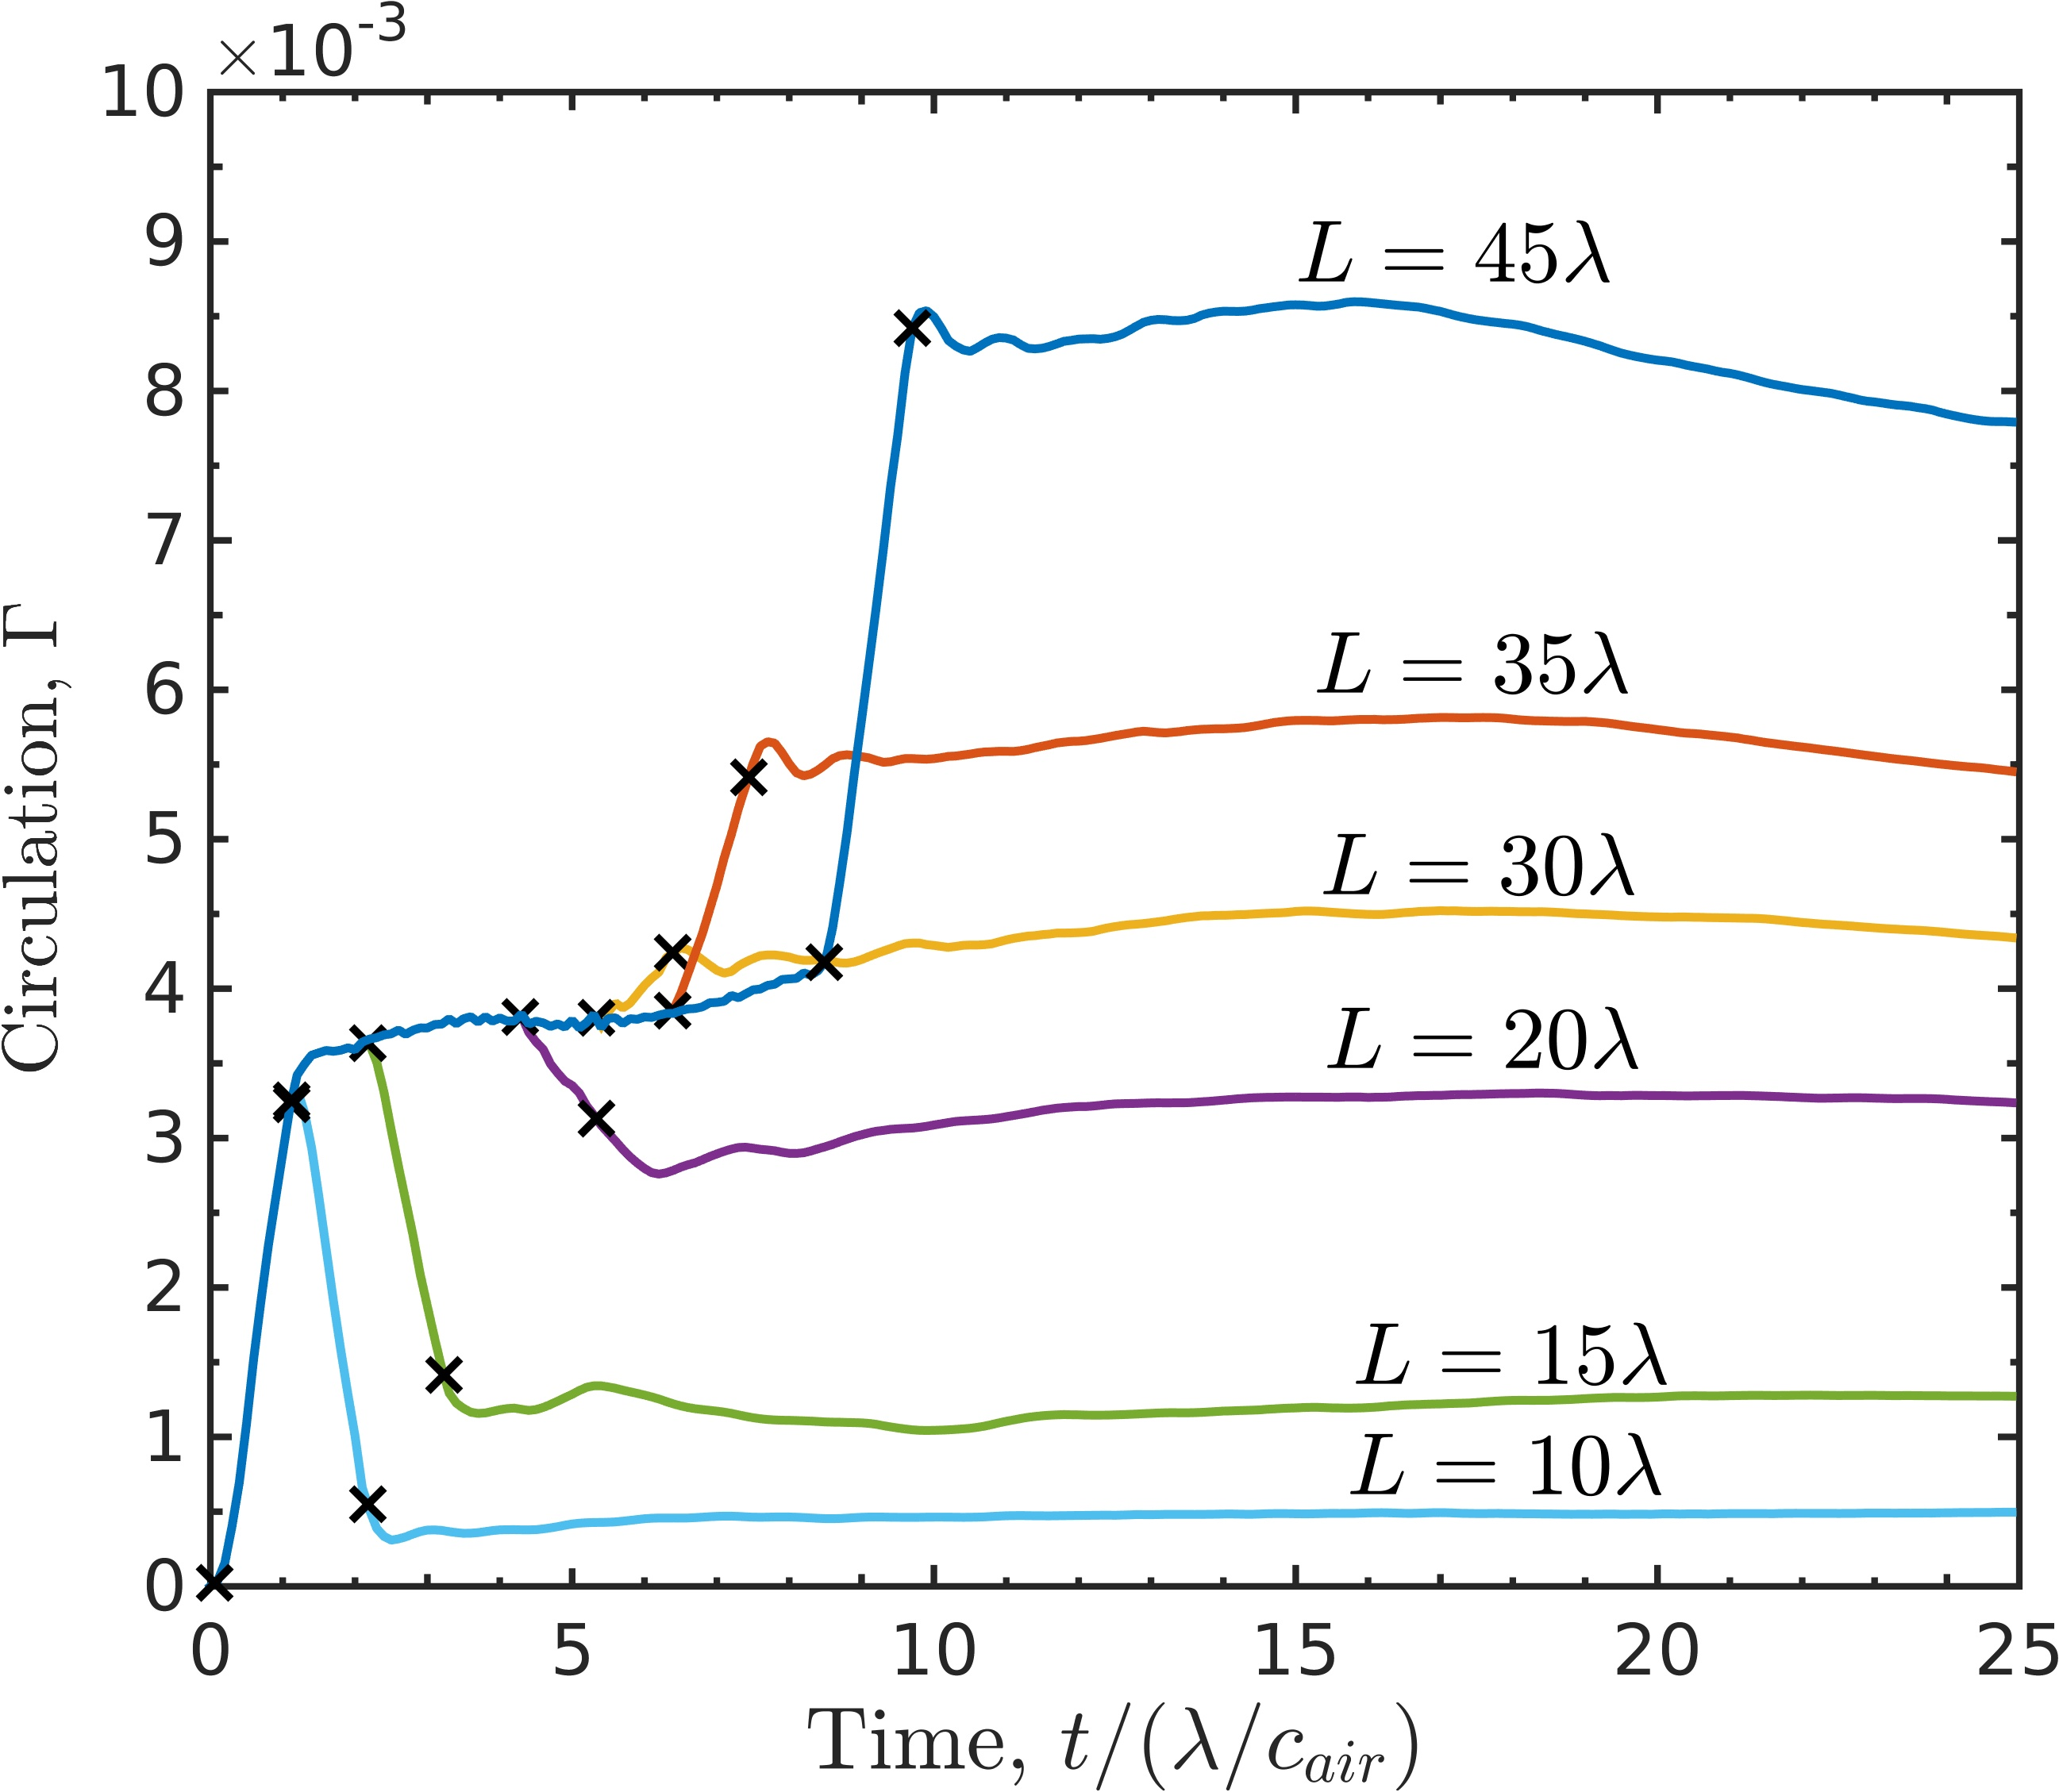
\includegraphics[width=0.48\textwidth]{./figs/lung_figs/circulation_multi-lag_fixed}
  \caption[The interface and circulation dependence on wave
  duration]{The interface amplitude (left) and circulation (right)
    histories for waves of varying total length $L$ and elevated
    static pressure duration between the expansion and compression
    . Here we show results for $L=45\lambda$ (blue), $L=35\lambda$
    (orange), $L=30\lambda$ (yellow), $L=20\lambda$ (purple),
    $L=15\lambda$ (green), $L=10\lambda$ (light blue)}
  \label{fig:trapz_circ_interface_multi-lag}
\end{figure}

\subsection{Interface response to \acf{DUS} waves}%
\label{subsec:usbe_lung_trapezoidal_results}%
To evaluate the relevance of our trapezoidal wave experiments we simulate
a $p_a=1, 5$ and $10$ MPa \ac{DUS} pulse waves (See Figure
\ref{fig:p0}) impinging onto the water air interface. In figure
\ref{fig:us_circ_interface} we illustrate the circulation and
interface amplitude histories for the $p_a=10$ MPa \ac{DUS} like-pulse
case. The post-wave interface dynamics are similar to those observed
for trapezoidal wave cases. During the wave-interface interaction, the
interface amplitude is compressed overall, but oscillations are
observed in correspondence with the acoustic pulse oscillations. After
the wave has left the interface, the perturbation amplitude continues
to decrease until the interface undergoes a phase inversion, after
which the perturbation amplitude grows for the remainder of the
simulation. half-domain circulation oscillates during wave-interface
interaction before settling to a nearly constant non-zero value after
the wave has passed. We note that the total circulation deposited is
of the same order of magnitude as that generated by the trapezoidal
wave of the same amplitude and duration. Qualitatively similar results
were observed for the $5$ MPa case. For the one $1$ MPa case, the
evolution of the system was slow such that running the simulation long
enough to obtain useful results was computationally prohibitive.

\begin{figure}
  \centering
  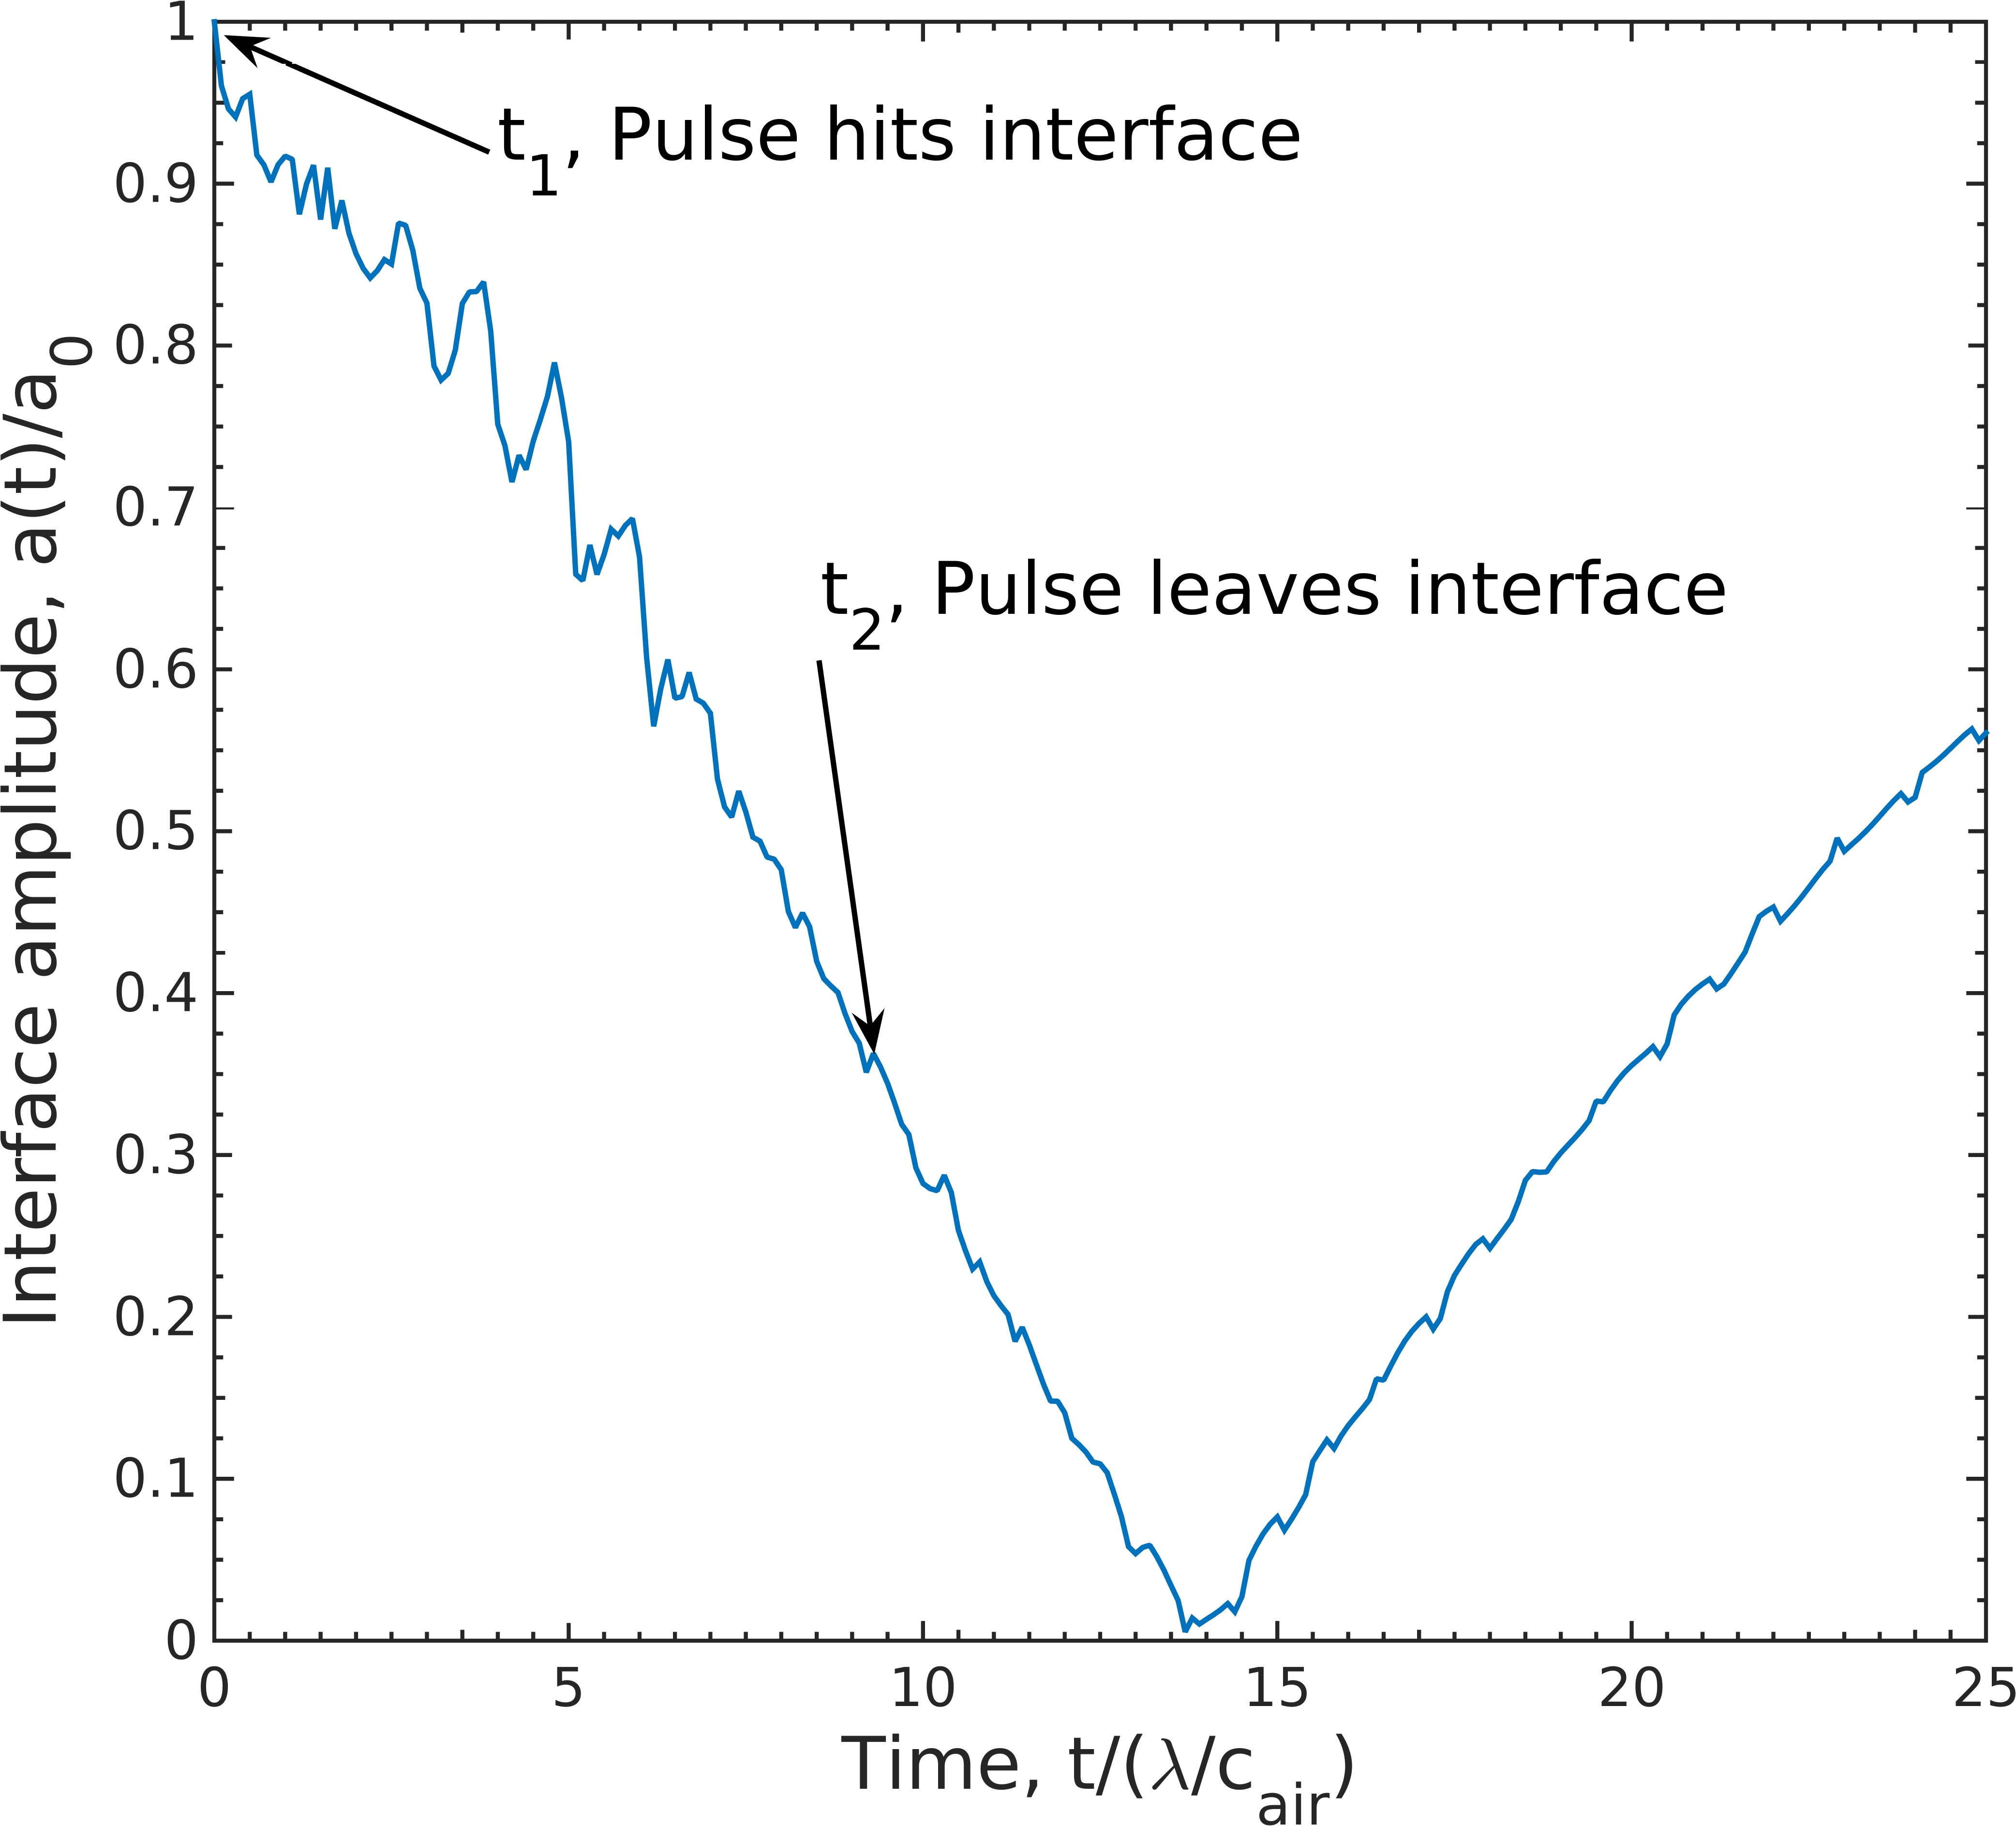
\includegraphics[width=0.48\textwidth]{./figs/lung_figs/us_intf_schematic} \hfill
  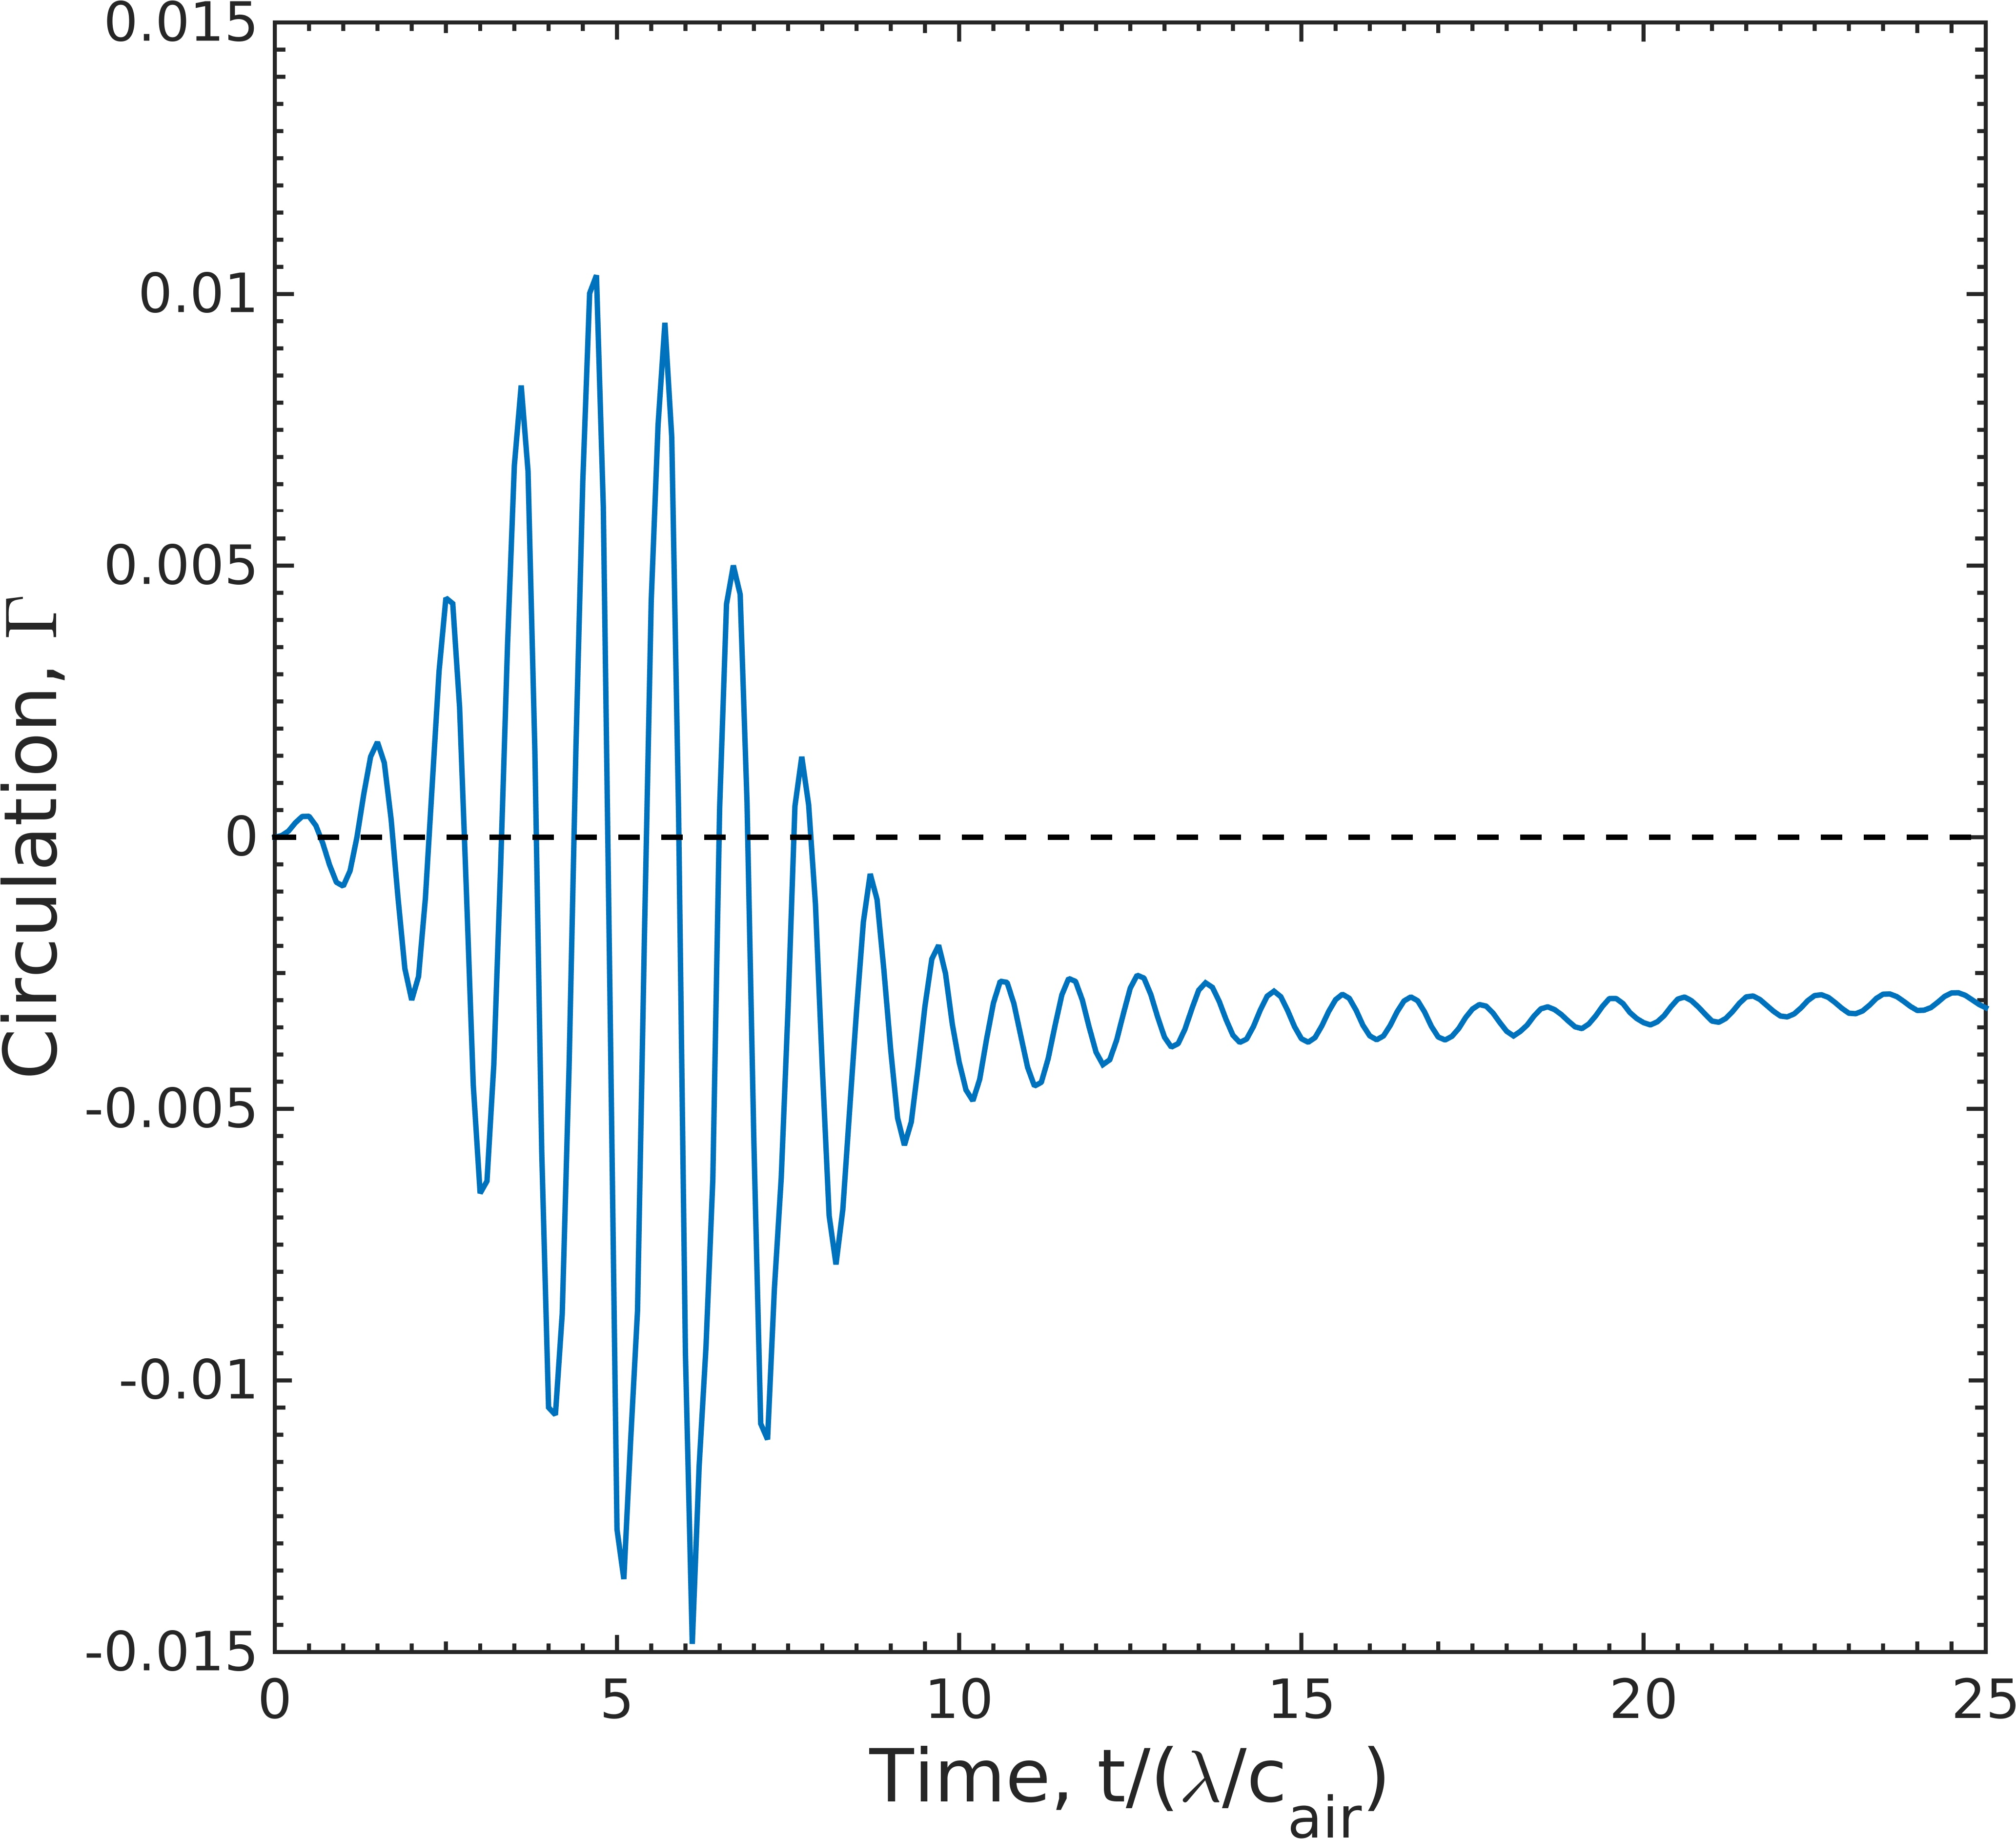
\includegraphics[width=0.48\textwidth]{./figs/lung_figs/us_circ_schematic}
  \caption[The interface amplitude and circulation histories for the \ac{DUS} pulse]{The interface amplitude (left) and circulation (right)
    histories corresponding to the a water-air interface disturbed by
    the US-like pulse shown in Figure \ref{fig:p0}.}
  \label{fig:us_circ_interface}
\end{figure}

\subsection{Further discussion of the results}%
\label{subsec:usbe_lung_further_discussion}%
For both the trapezoidal and \ac{DUS} pulse acoustic waves, the
pressure, velocity, and density return to initial, ambient conditions
after the passing of the wave. As these waveforms are continuous, this
implies that the integral of the pressure gradient $\nabla p$ at each
point along the interface, over all time must be zero. Hence we
surmise that if the interface remains unchanged during the interaction
with the wave, as it would for a wave moving with infinite velocity,
$\nabla \rho$ remains constant and the net baroclinic circulation
deposited must be zero. Thus for any finite duration acoustic wave
such as ours to deposit net baroclinic circulation upon an interface,
the interface itself must deform during interaction with the
wave. This deformation alters the misalignment of the pressure and
density gradients at the interface causing positive and negative
circulation deposited to not cancel out entirely. Note that this is
unique to waves that begin and end at the same pressure. This is not
the case for the traditional \ac{RMI} problem, for which conditions do
not return to their original state after the passage of the shock.

For the cases varying the length of the static elevated pressure in
the trapezoidal wave we previously noted that whether the expansion
increased or decreased the total half-domain circulation depended on
whether it encountered the interface before or after the phase
change. If indeed circulation is driving the deformation of the
interface, then changes in the waveform that appear to have very
little effect on the interface dynamics during the wave-interface
interaction period, may have far more significant impacts on the long
term dynamics of the interface. To put this in the context of
\ac{DUS}, which uses repeated pulses, if ultrasonically-deposited
circulation is causing deformation within the lungs, longer \acp{PD}
may allow for greater deformation and increased circulation deposition
as a result of any individual pulse. If the system acts as we have
modeled it, the \ac{PRF} would determine the degree of interface
deformation experienced by pulses subsequent to the first and may
influence deformation and hemorrhage. Finally, in recognition of the
limitations of this study, we note that the true physical nature of
lung tissue is viscoelastic \citep{Bayliss1939}, and neither viscosity
nor elasticity is included in our model problems. While preliminary
results with a Navier-Stokes code showed similar early time results,
we expect that viscosity would dissipate circulation over a long
enough period of time. Furthermore, elasticity may provide a mechanism
by which the alveolar walls could resist deformation or retard to
their original shape between pressure perturbations.

In the context of \ac{DUS}, which uses repeated pulses, if
ultrasonically-deposited circulation is causing deformation within the
lungs, longer \acp{PD} may allow for greater deformation and increased
circulation deposition as a result of any individual pulse. If the
system acts as we have modeled it, the \ac{PRF} would determine the
degree of interface deformation experienced by pulses subsequent to
the first and may influence deformation and hemorrhage. Finally, in
recognition of the limitations of this study, we note that the true
physical nature of lung tissue is viscoelastic \citep{Bayliss1939},
and neither viscosity nor elasticity is included in our model
problems. While preliminary results with a Navier-Stokes code showed
similar early time results, we expect that viscosity would dissipate
circulation over a long enough period of time. Furthermore, elasticity
may provide a mechanism by which the alveolar walls could resist
deformation or retard to their original shape between pressure
perturbations.



%-----------------------------------------------------------------------


% %
% In this section we present the results of the numerical experiments
% and compare them to our analysis. We briefly touch on the general
% behavior of the acoustic waves, during the experiments, then go on to
% discuss the interface dynamics associated with the trapezoidal
% acoustic waves. We present results to illustrate the behavior of the
% interface during and after interactions with the acoustic waves. We
% compare the late time interface growth to the scaling law we obtained
% for purely circulation-driven interface growth based on dimensional
% analysis (Relationship \eqref{eq:intf_circ_scaling}). We additionally
% provide plots of the half-domain circulation as a function of time and
% contours of vorticity to show that the compression and expansion waves
% deposit vorticity at the interface. We further plot the individual
% advective, compressible, and baroclinic contributions
% \eqref{eq:circulation_generation_components} to the circulation
% generation equation \eqref{eq:circulation_generation} as functions of
% time to demonstrate the specific physical mechanisms responsible for
% generating circulation at teach stage of the interaction. We next
% investigate the dependence of the interface and circulation dynamics
% on the time dependent features of the wave by varying the lag time
% between the compression and expansion portions of the trapezoidal
% wave. Then we present circulation and interface results for the
% \ac{US} pulse waveform case for comparison to the trapezoidal
% wave cases. Lastly, we discuss broadly some of the implications of the
% results as a whole.

% \subsection{Acoustic wave behavior}

% Trapezoidal and \ac{US} pulse waves (see Figure \ref{fig:p0})
% propagate from water toward the perturbed water-air interface. Nearly
% all ($>99.99\%$) of the acoustic energy is reflected back into the
% water. The sign of the reflected wave is opposite that of the incoming
% wave due to the movement of the incoming wave from media of higher to
% lower acoustic impedance, or simply, compression waves reflect
% expansion waves and vice versa. Due to the strong impedance mismatch,
% a very much weakened acoustic wave, with shape similar to the initial
% acoustic wave condition, is transmitted into the air. The curvature of
% the interface combined with the sound speed change across the
% interface causes slight redirection of the transmitted wave in
% accordance with Snell's law. Reflected and transmitted waves dissipate
% at the inflow and outflow boundaries.

% \subsection{Interface response to trapezoidal acoustic waves} \label{subsec:usbe_lung_trapz_results}
% \subsubsection{Qualitative observations for the $p_a=10$ MPa trapezoidal wave case}
% We first show typical interface amplitude and circulation histories to
% provide a qualitative understanding of the physics. For each
% trapezoidal wave case we observe that the interface begins to compress
% (i.e., the interface amplitude $a(t)$ decreases) when contacted by the
% wave and continues to deform throughout and after the interface-wave
% interaction period. At some point during this process the perturbation
% undergoes a phase change and the begins to grow in amplitude. This is
% consistent with the previously discussed \ac{RMI} for the case of a
% shock moving from a heavy fluid to a light fluid.

% To illustrate the evolution of the interface Figure
% \ref{fig:interface_snapshots} shows snapshots of the density (Top) and
% vorticity (Bottom) fields at different points in the flow's evolution
% for the case of a $10$ MPa trapezoidal wave impinging on the water-air
% interface. In the density plots, areas of high density (i.e., water)
% are dark blue and areas of low density (i.e., air) are white. From
% these contours we see that the initially smooth interface perturbation
% grows from a smooth sinusoid to a sharp spike at late time. On the
% vorticity contours, positive (counterclockwise) vorticity is red, and
% negative (clockwise) vorticity is blue.  When we compare the density
% and vorticity contours, we see that the vorticity is heavily
% concentrated in the air and remains so throughout the flow.

% Figure \ref{fig:trapz10_circ_interface} shows the
% early-time interface amplitude and half-domain circulation histories
% for the same case. At $t_1=0^+$ the compression portion of the wave
% first hits the interface. The interface begins to compress and the
% perturbation amplitude decreases. From $t_1$ to $t_2$ the half-domain
% circulation $\Gamma$ rises sharply. At $t_2\approx1.1$, the
% compression portion of the wave has passed, the interface amplitude
% continues to decrease. The half-domain circulation $\Gamma$ stops its
% rapid growth and changes little during this static elevated pressure
% period, until the expansion wave hits at $t_3$. At $t\approx 5.0$, the
% perturbation undergoes a phase inversion and begins to grow. At
% $t_3\approx8.5$ the expansion wave first hits the interface. The
% perturbation amplitude continues to grow, and $\Gamma$ increases
% sharply again. At $t_4\approx9.7$ the acoustic wave has finished
% traversing the interface, and atmospheric pressure is resumed.
% %
% \begin{figure}[h] 
%   \centering
% 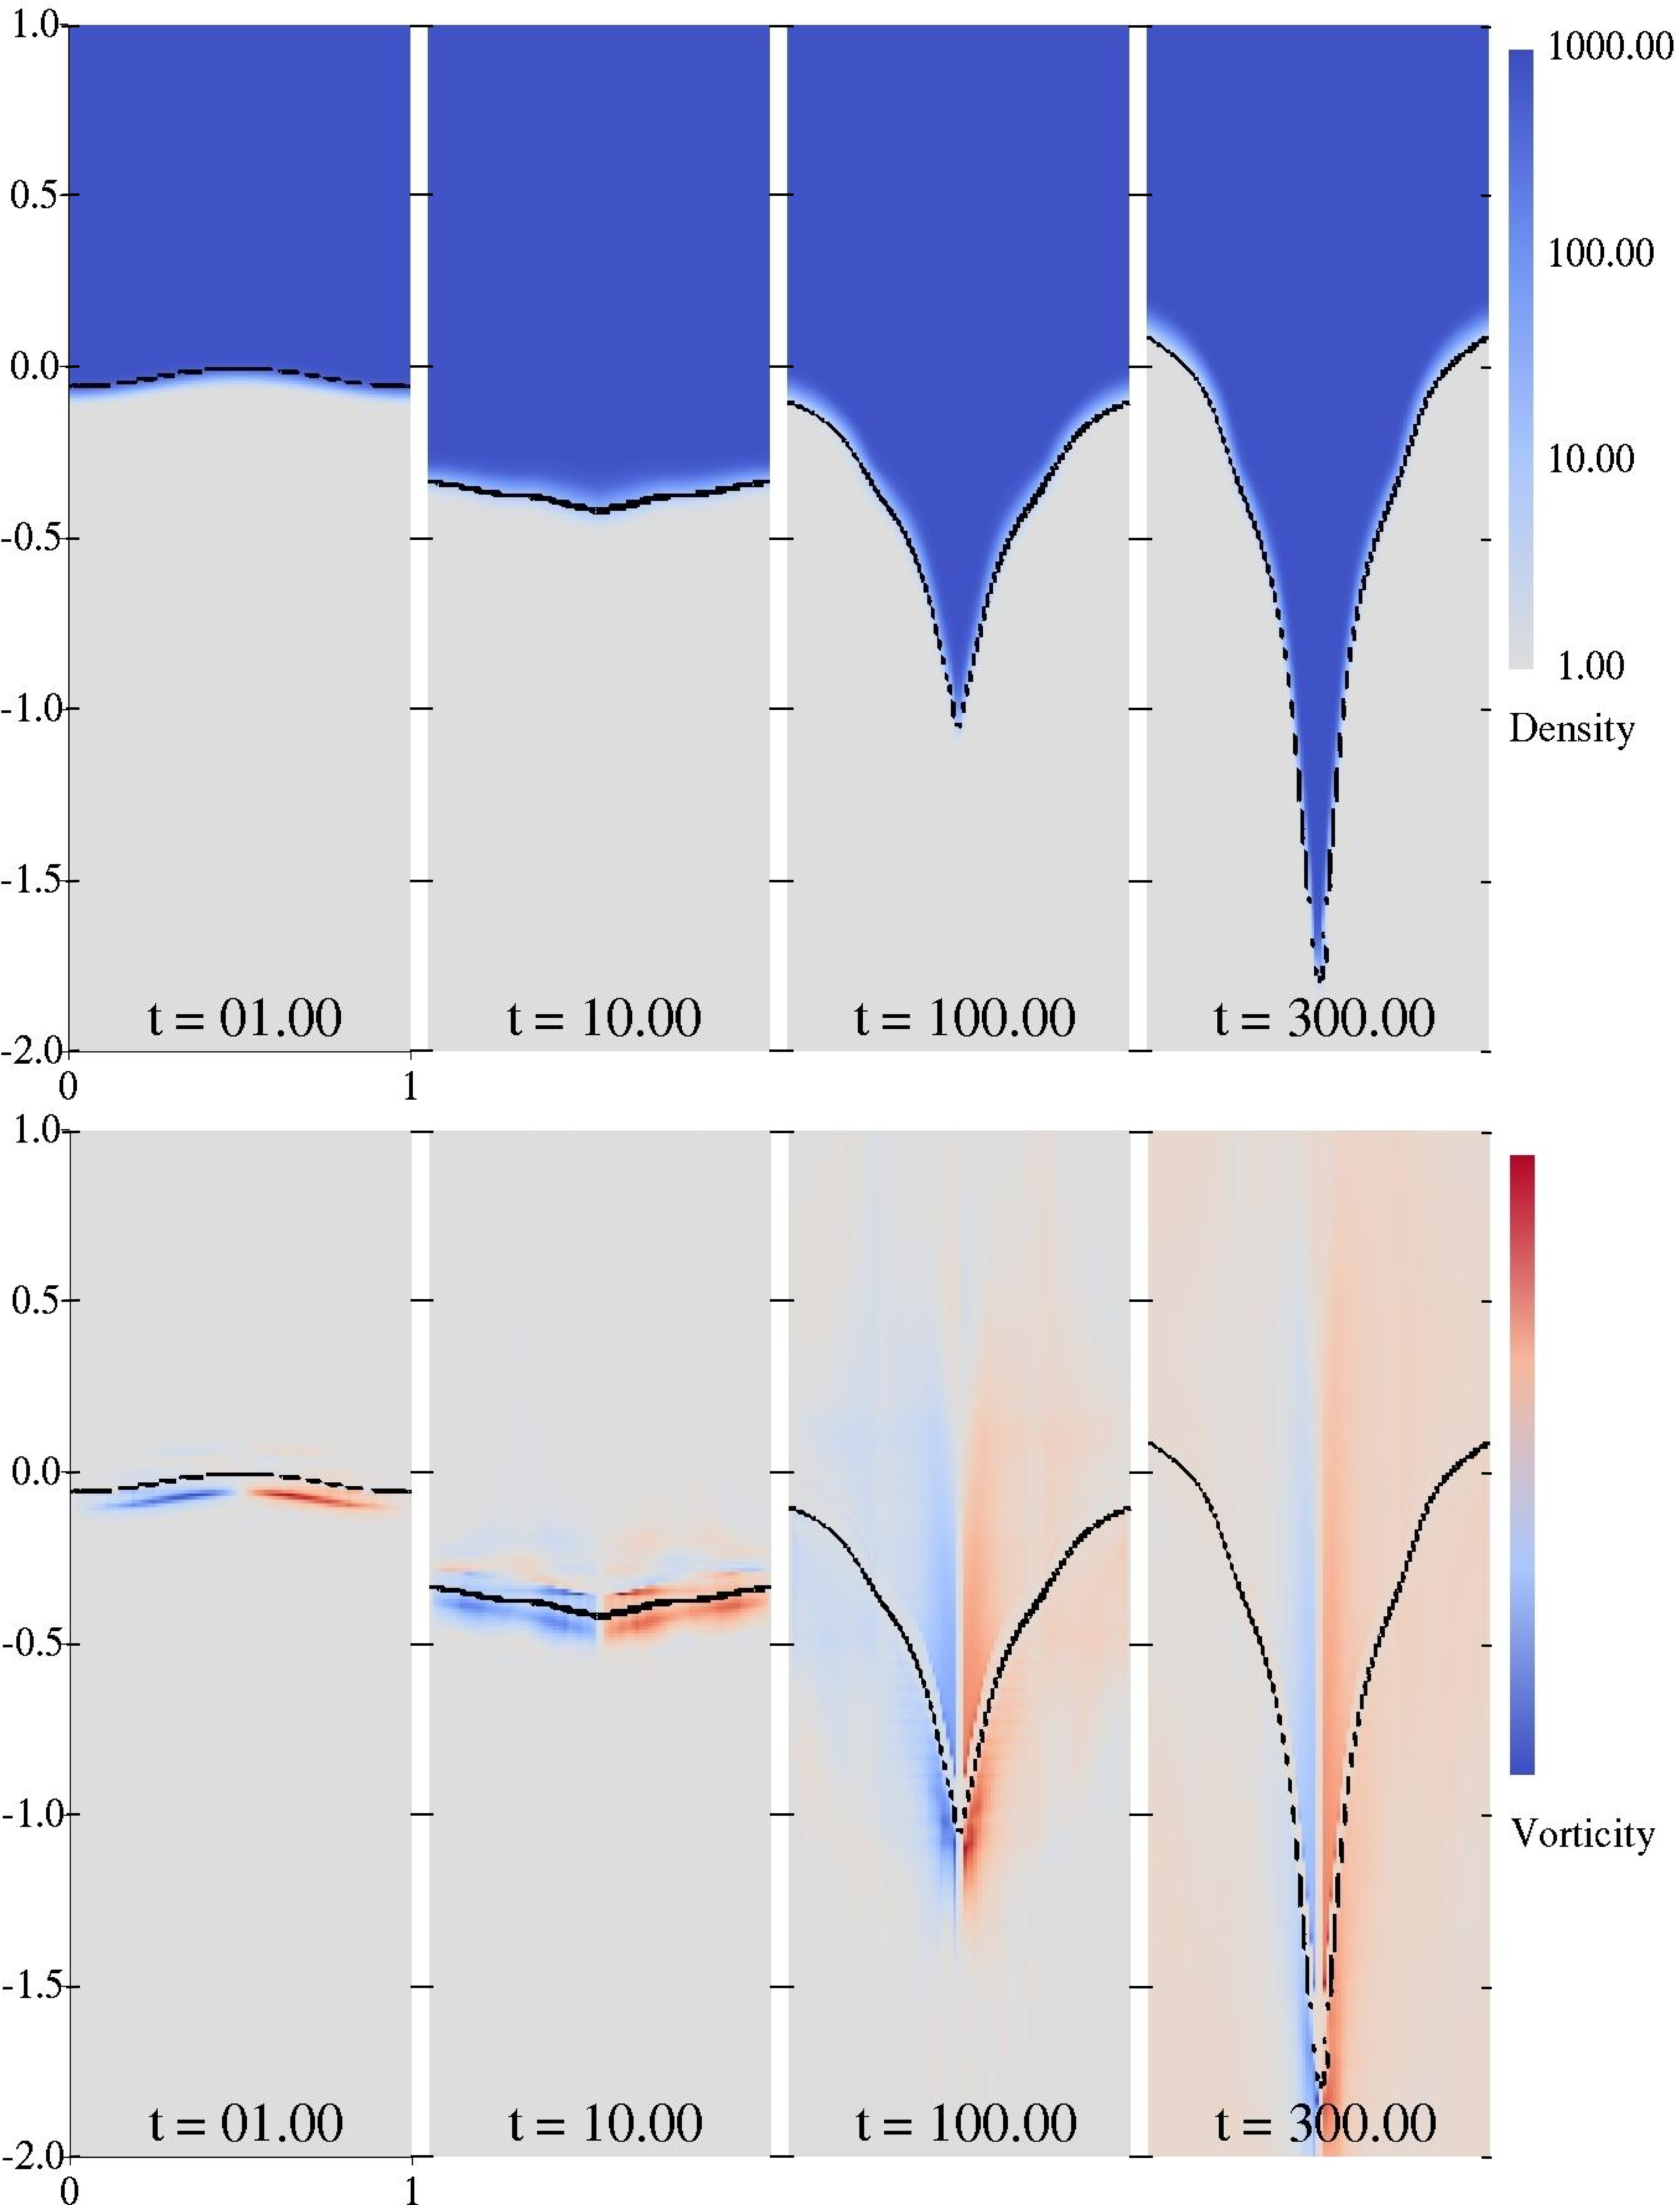
\includegraphics[width=0.9\textwidth]{./figs/lung_figs/snapshots_t1}
% \caption[The evolution of the acoustically perturbed interface and vorticity field]{Surface plots of density (Top) and vorticity (Bottom)
%   throughout the evolution of the interface for the $10$ MPa
%   trapezoidal wave case. Areas of high density (i.e., water) are
% indicated in dark blue. Areas of low density (i.e., air) are indicated
% in white.  Positive (counterclockwise) vorticity is indicated in red,
% and negative (clockwise) vorticity can be seen in blue.}
%   \label{fig:interface_snapshots}
% \end{figure}
% %
% \begin{figure}[h] 
%   \centering
%   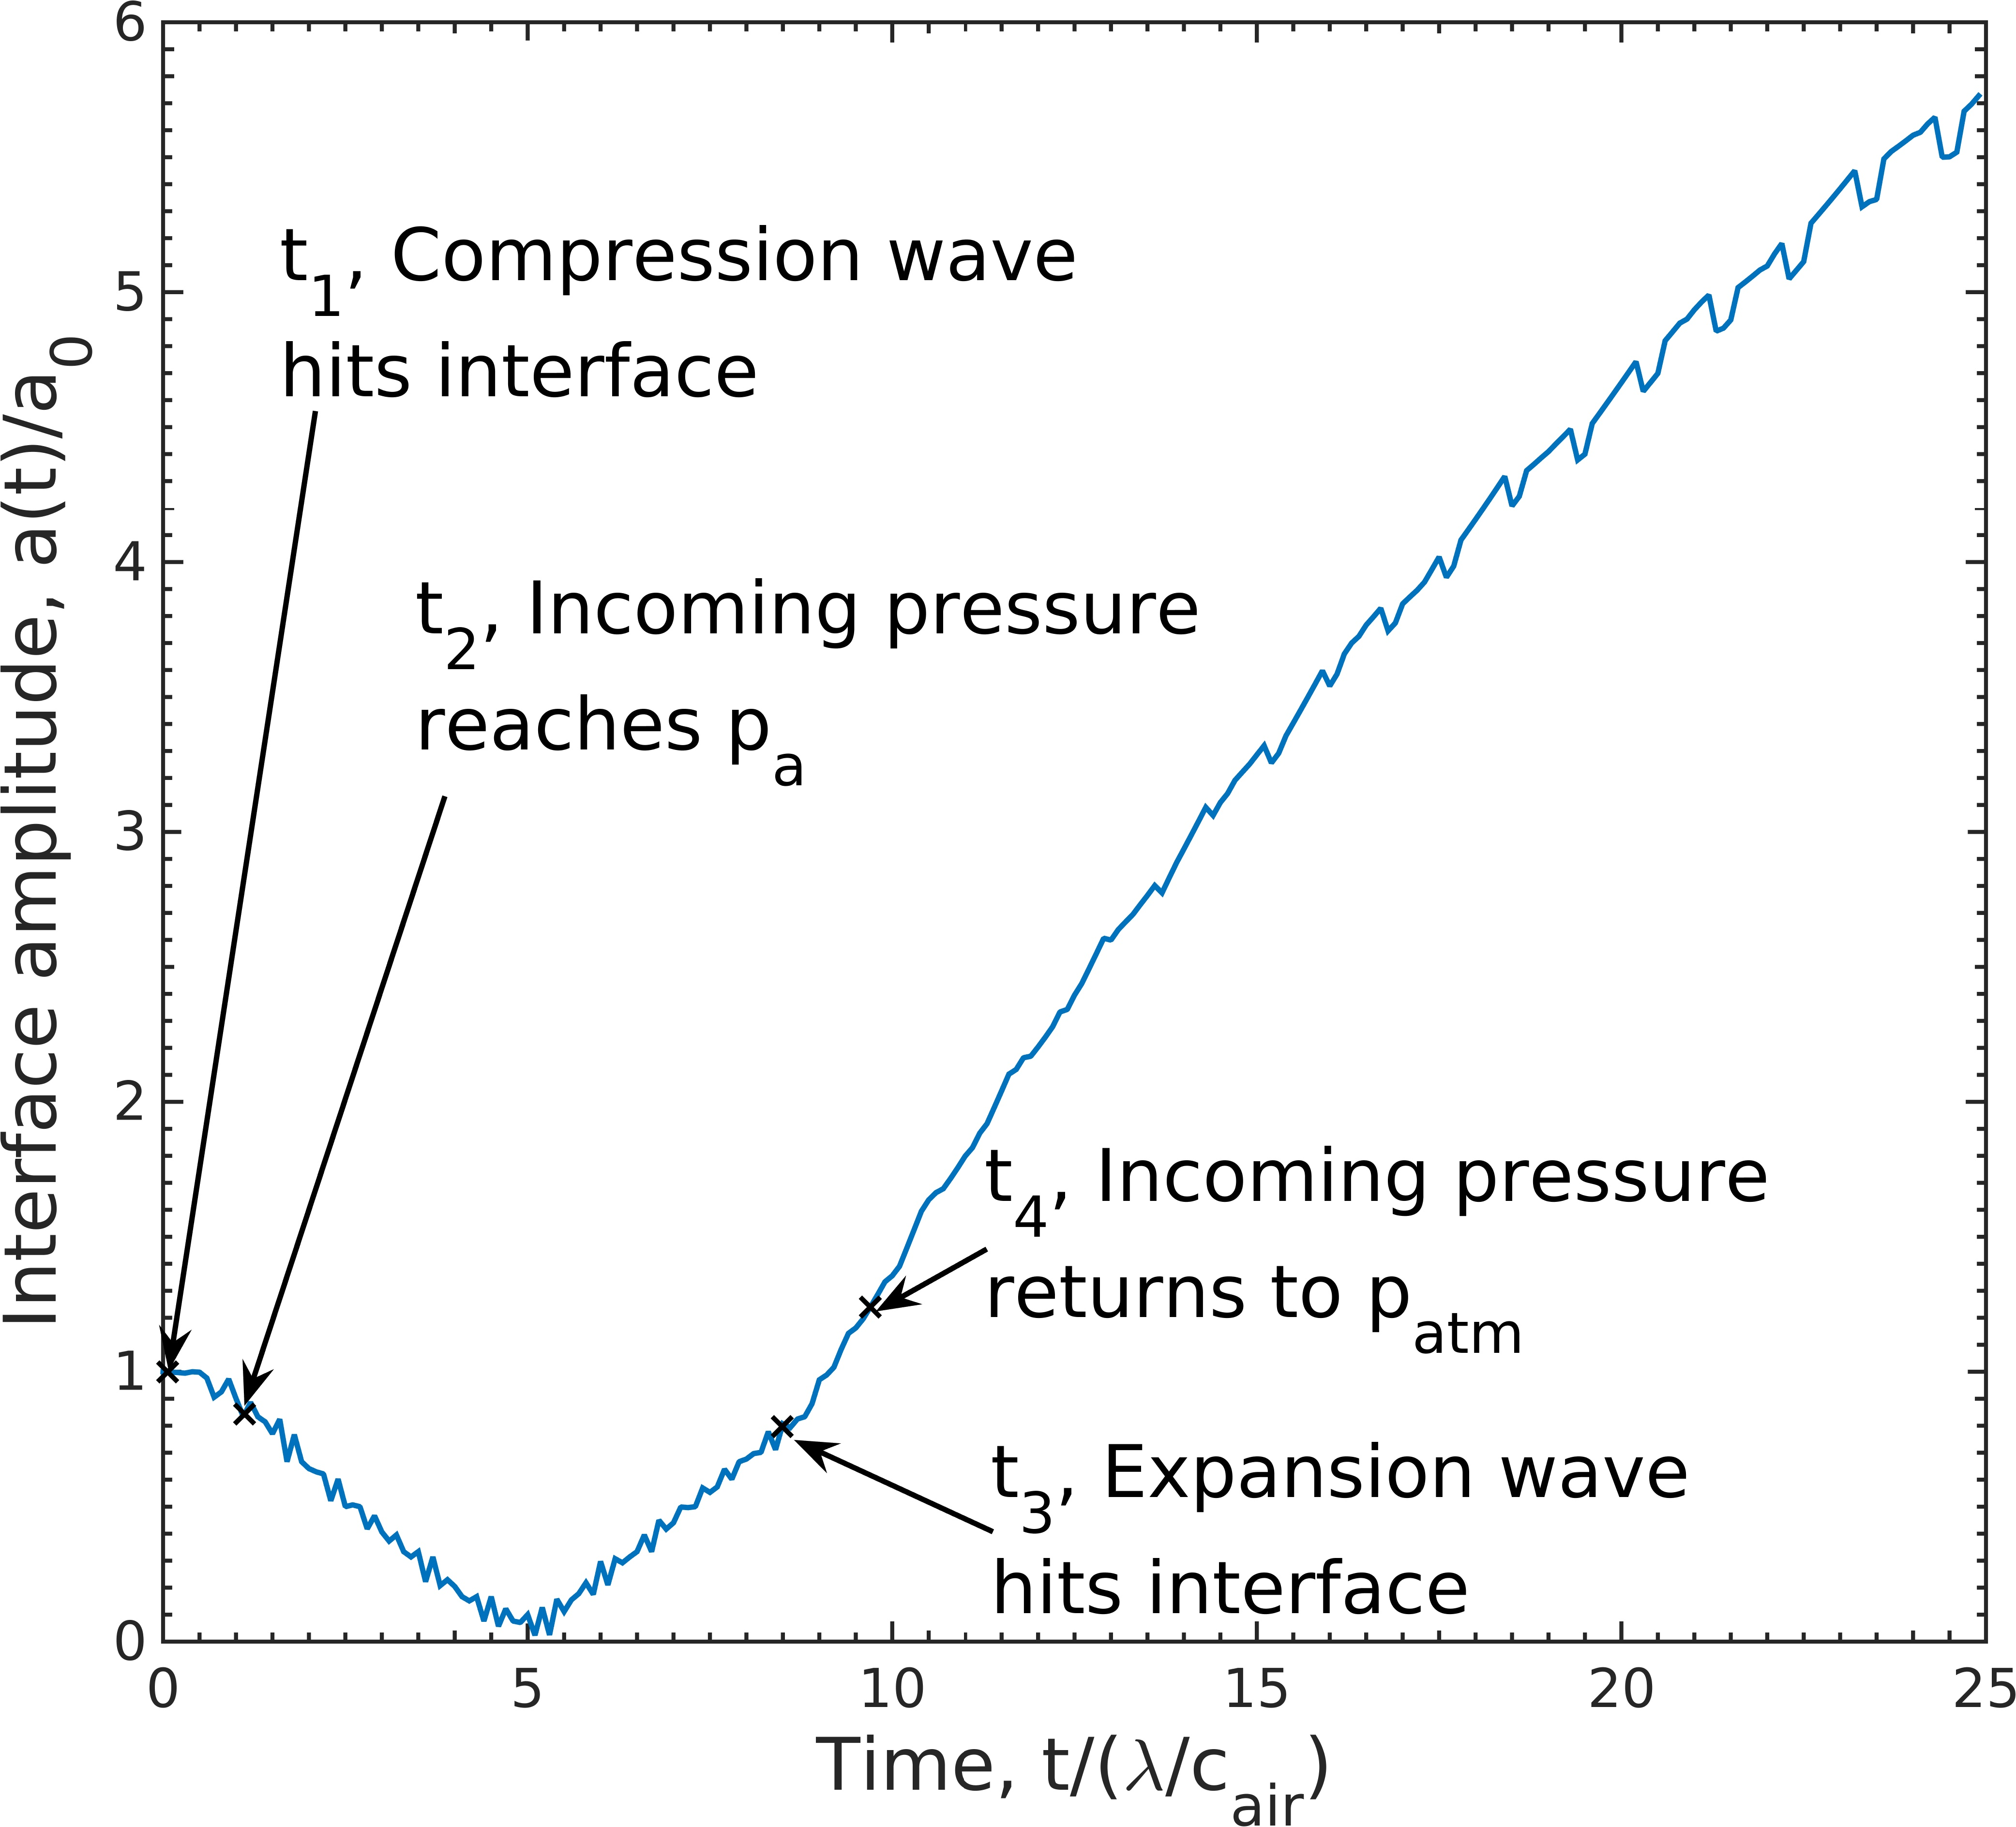
\includegraphics[width=0.48\textwidth]{./figs/lung_figs/trapz10_intf_schematic}
%   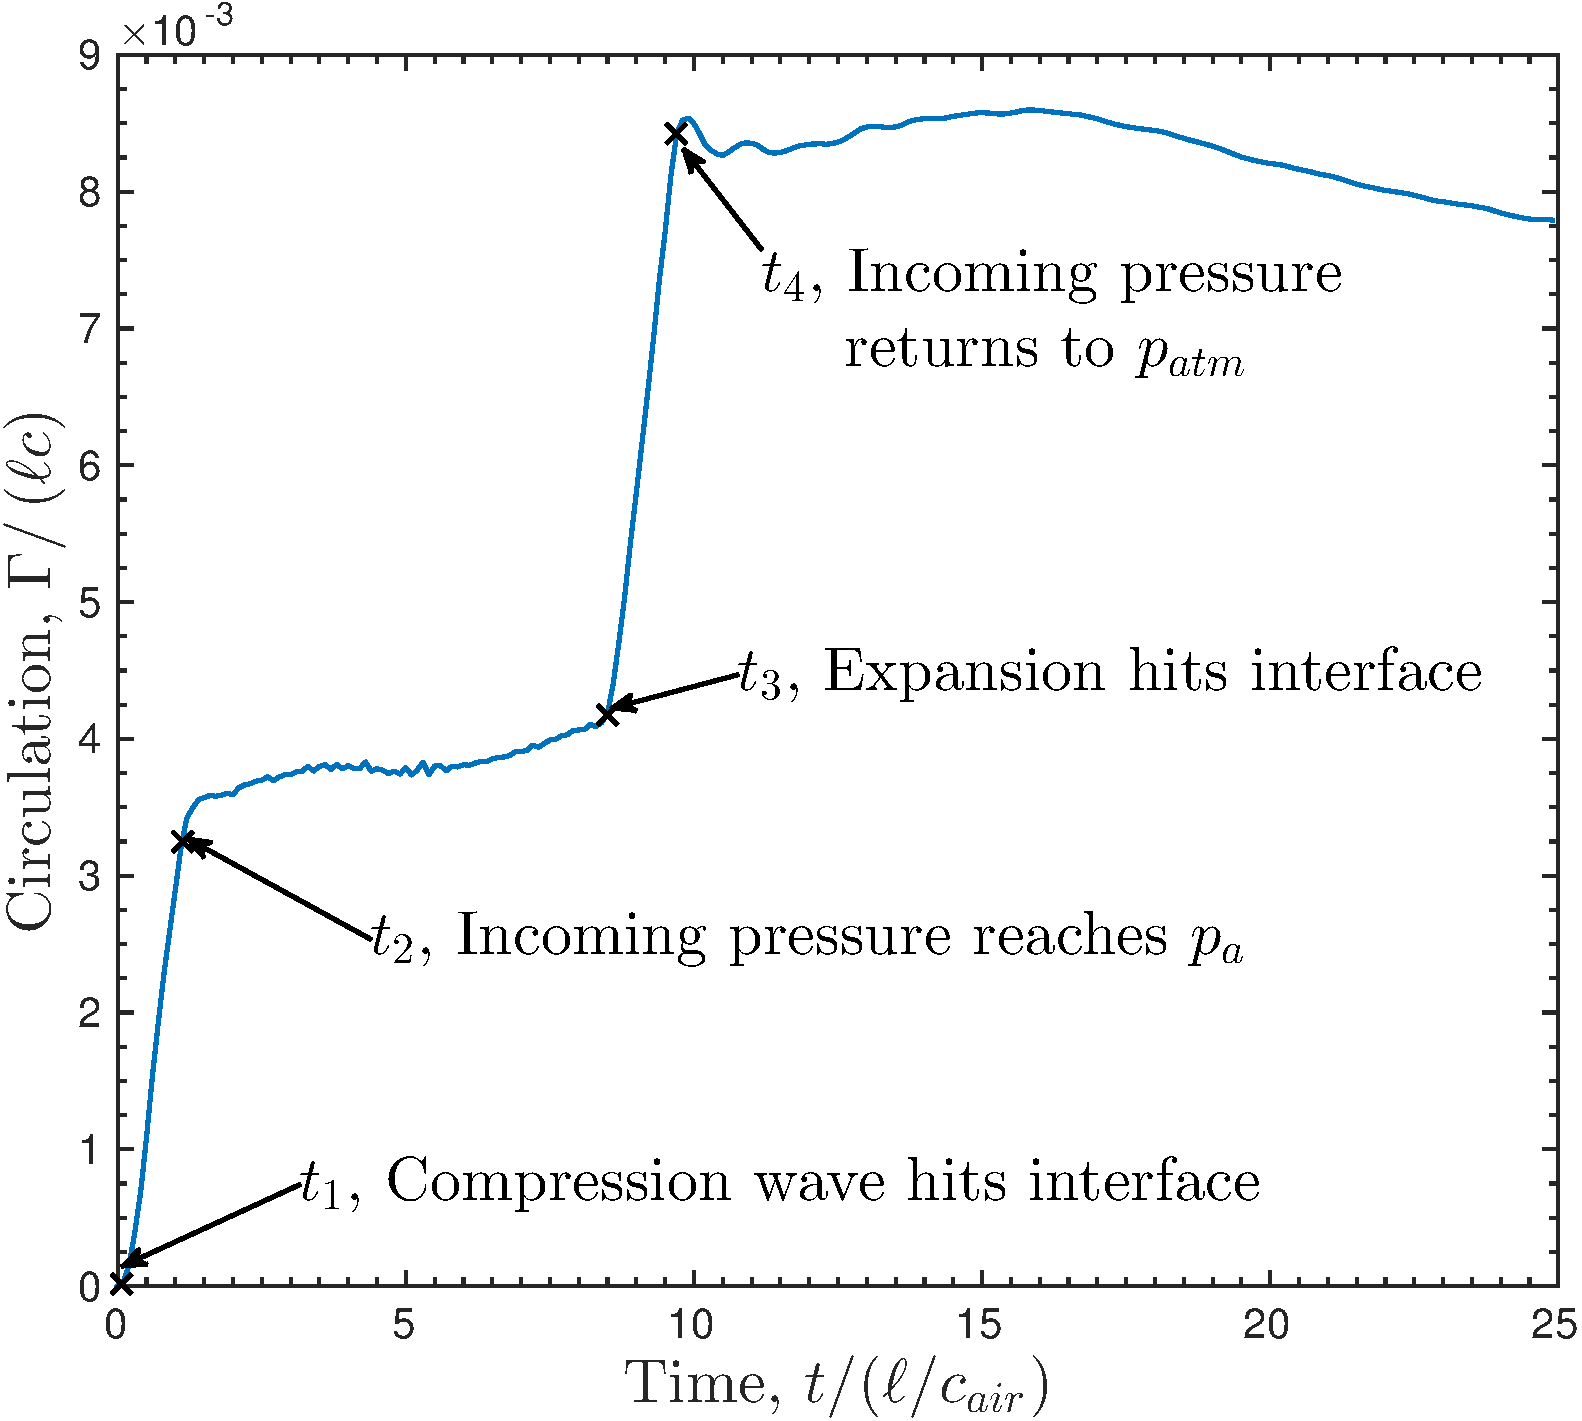
\includegraphics[width=0.48\textwidth]{./figs/lung_figs/trapz10_circ_schematic}
%   \caption[The interface amplitude and circulation histories for the $10$ MPa trapezoidal wave]{The interface amplitude (left) and circulation (right)
%     histories corresponding to the $10$ MPa trapezoidal waves are
%     shown for $t\leq25$. Indicated times, $t_{1-4}$, are the times at
%     which different stages of the incoming trapezoidal pressure wave
%     shown in Figure \ref{fig:p0} first encounter the interface.}
%   \label{fig:trapz10_circ_interface}
% \end{figure}
% %
% \subsubsection{Dependence on wave amplitude}%
% \label{subsubsec:usbe_lung_amplitude_dependence}%
% To illustrate the effects of varying the trapezoidal wave amplitude,
% while keeping the duration of each wave feature constant, we show
% interface amplitudes and half-domain circulation histories for
% $p_a=1$, $5$, and $10$ MPa trapezoidal waves. In Figure
% \ref{fig:trapz_circ_interface_early}, we look closely at the period
% around the wave interaction for $0 \leq t\leq 25$. We note that the
% for the $p_a10$ MPa case, the phase reversal of the interface happened
% around $t=5.0$, which is about haft the time it took for this to occur
% for the for the $p_a=5$ MPa case. The $p_a1$ MPa case, the evolution
% of the interface is sufficiently slow as to not phase invert during
% the period shown. For each wave amplitude, the circulation is
% normalized by the $p_a$ to show that the circulation generated by the
% interface-compression wave interaction, $0^+<t<scales<0.12$, increases
% linearly with $p_a$. To show the longer term effects of varying
% amplitude and show the late time behavior of the interface, defined as
% the behavior significantly after the acoustic waves have left the
% domain, Figure \ref{fig:trapz_circ_interface_loglog} shows the
% interface amplitude and half-domain circulation histories for
% $0 \leq t\leq 500$ as functions of time for $5$ and $10$ MPa
% trapezoidal waves impinging on the interface. Here, the interface
% amplitude is plotted on logarithmically-scaled axes. From scaling law
% \eqref{eq:intf_circ_scaling} we expect that for purely circulation
% driven interface growth, $a(t)$ will grow with $\sqrt{t}$, which is
% shown by dashed lines of corresponding colors. For the $10$ MPa wave
% case the slope of the observed growth appears to grow as $t^{0.6}$.
% Longer time simulations will be used to see if this settles to the
% expected $\sqrt{t}$ growth. Note that results for the $1$ MPa
% trapezoidal wave were not included because the slow evolution of the
% interface made the computation prohibitively expensive.
% %
% \begin{figure}[h] 
%   \centering
%   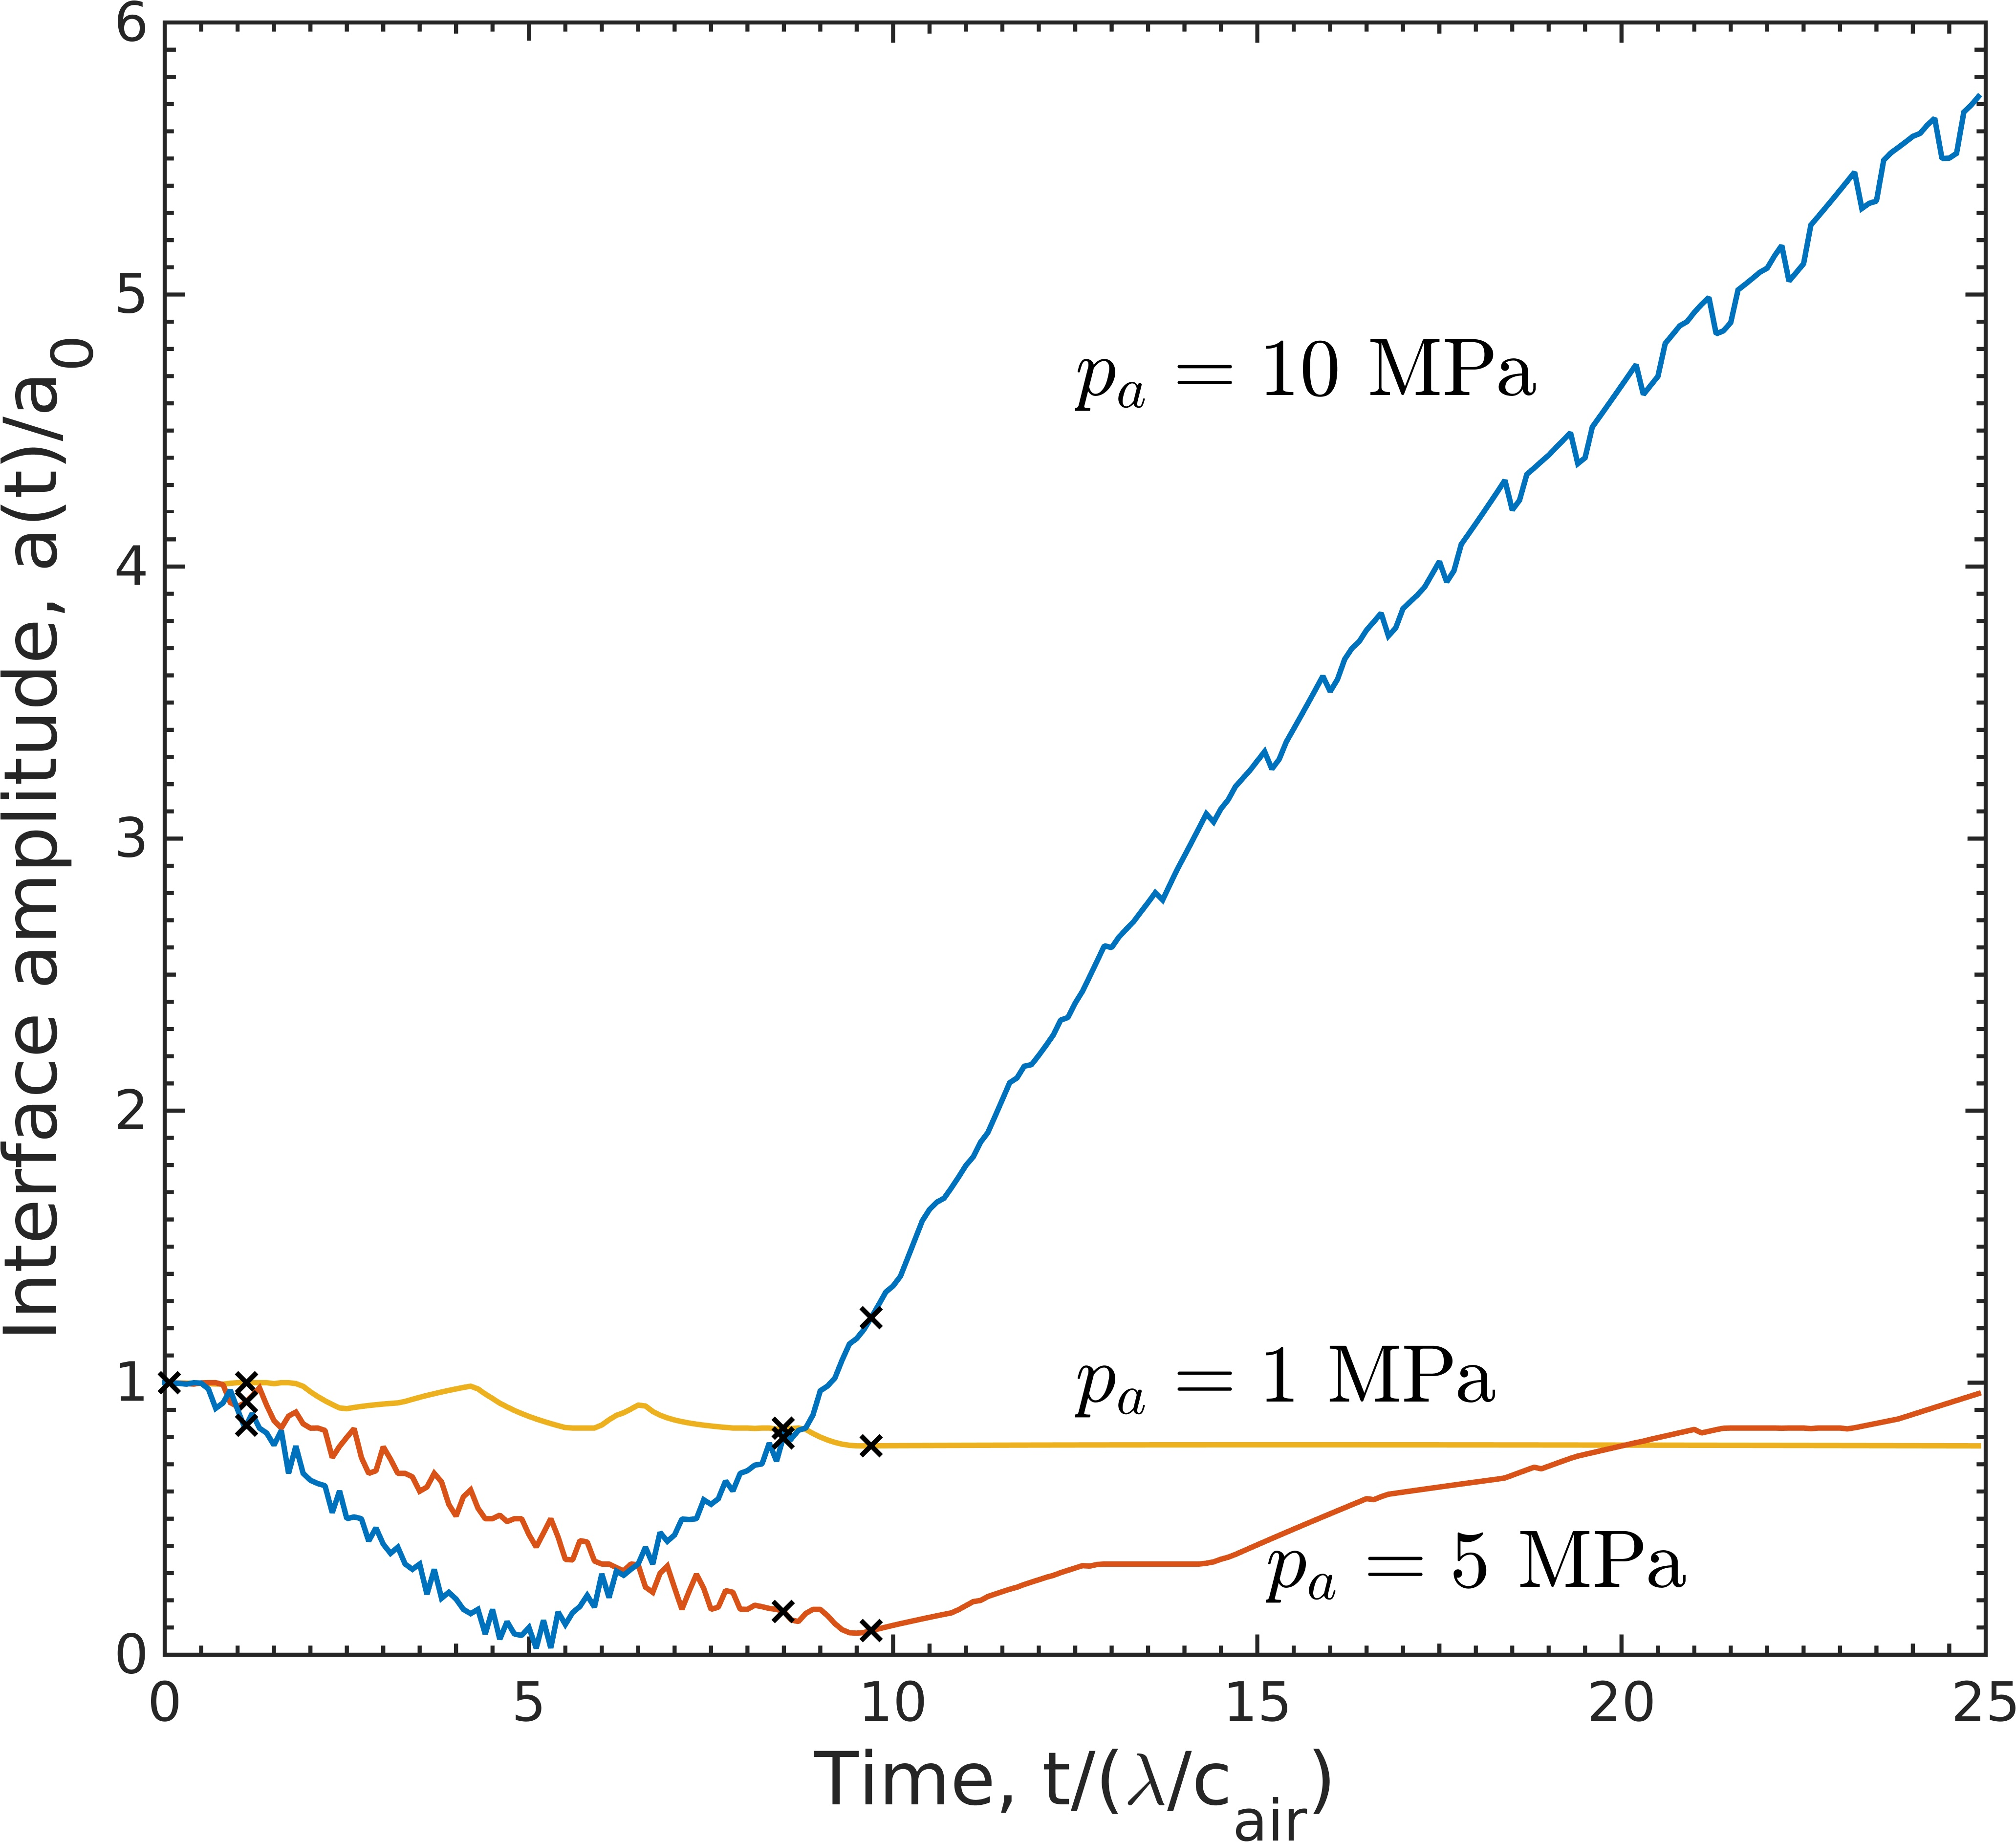
\includegraphics[width=0.48\textwidth]{./figs/lung_figs/interface_multi-amp_norm}
%   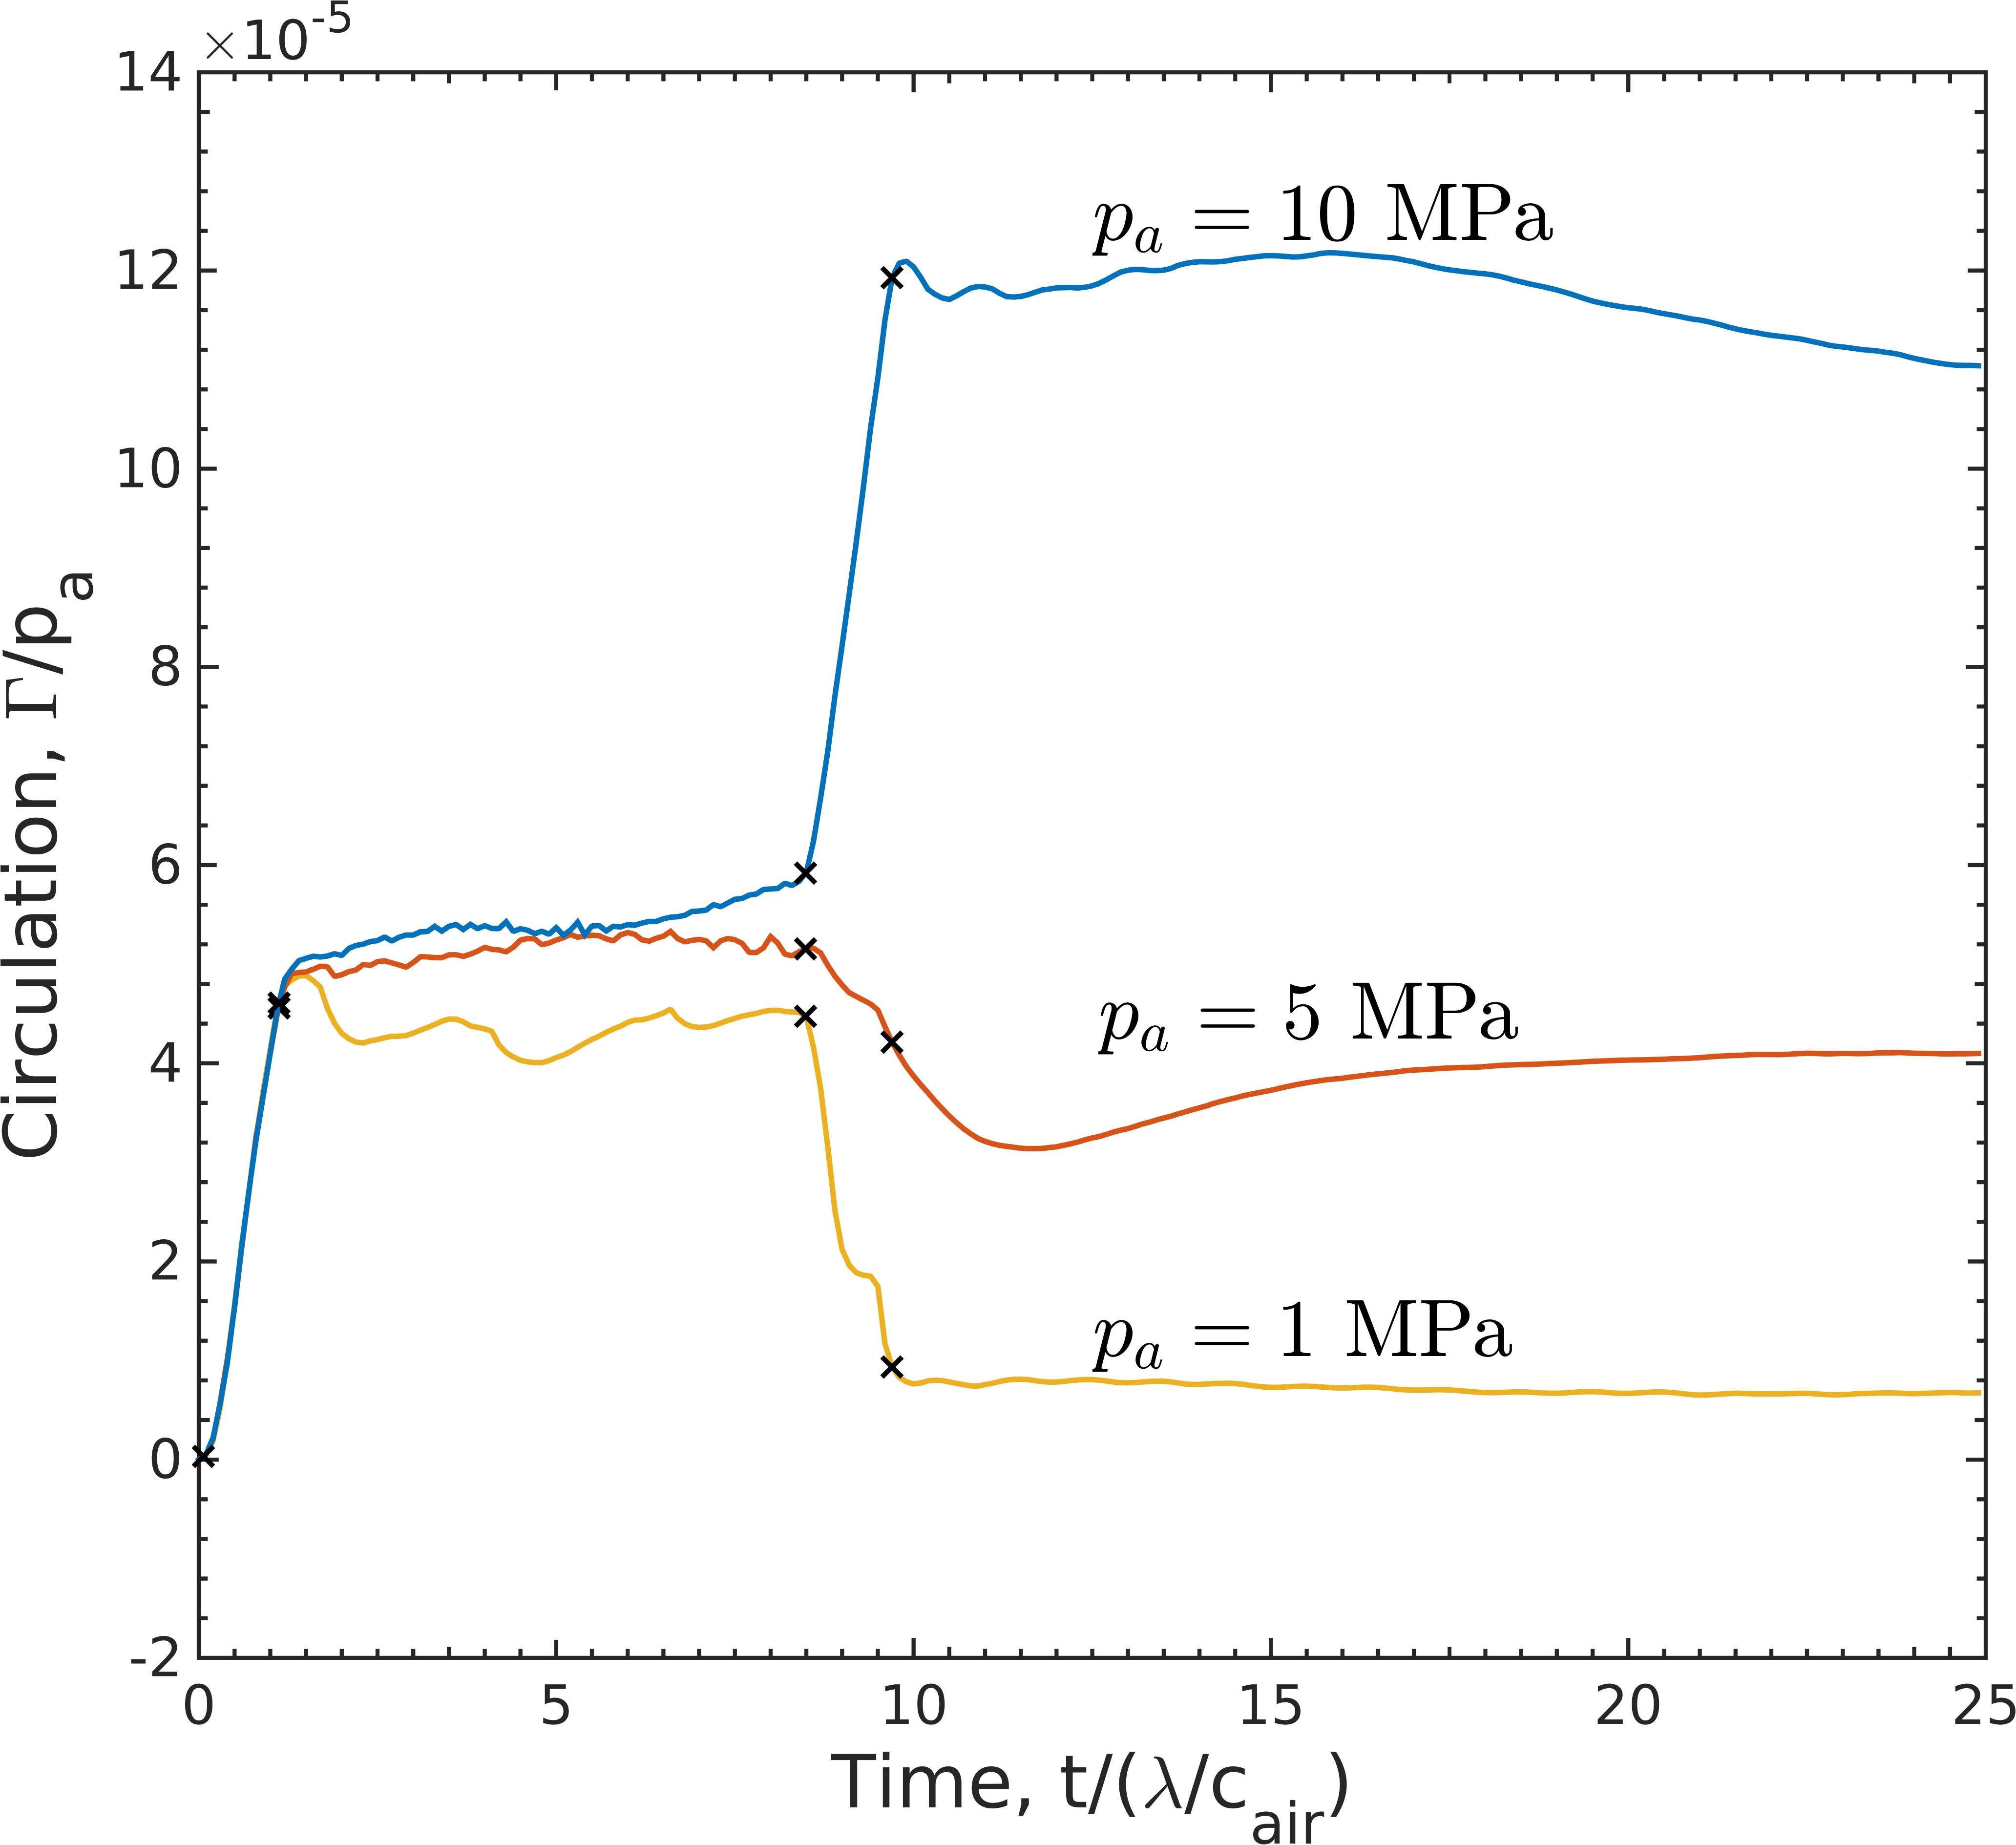
\includegraphics[width=0.48\textwidth]{./figs/lung_figs/circulation_multi-amp_norm}
%   \caption[The interface and circulation dependence on wave amplitude at early time]{The interface amplitude (left) and circulation (right)
%     histories corresponding to the $1$(yellow), $5$(orange), and
%     $10$(blue) MPa trapezoidal waves are shown for $t\leq 25$. The
%     circulation history is normalized by the acoustic amplitude of the
%     incoming wave to illustrate that circulation deposition by the
%     compression wave scales linearly with $p_a$ }
%   \label{fig:trapz_circ_interface_early}
% \end{figure}
% %
% \begin{figure}[h] 
%   \centering
%   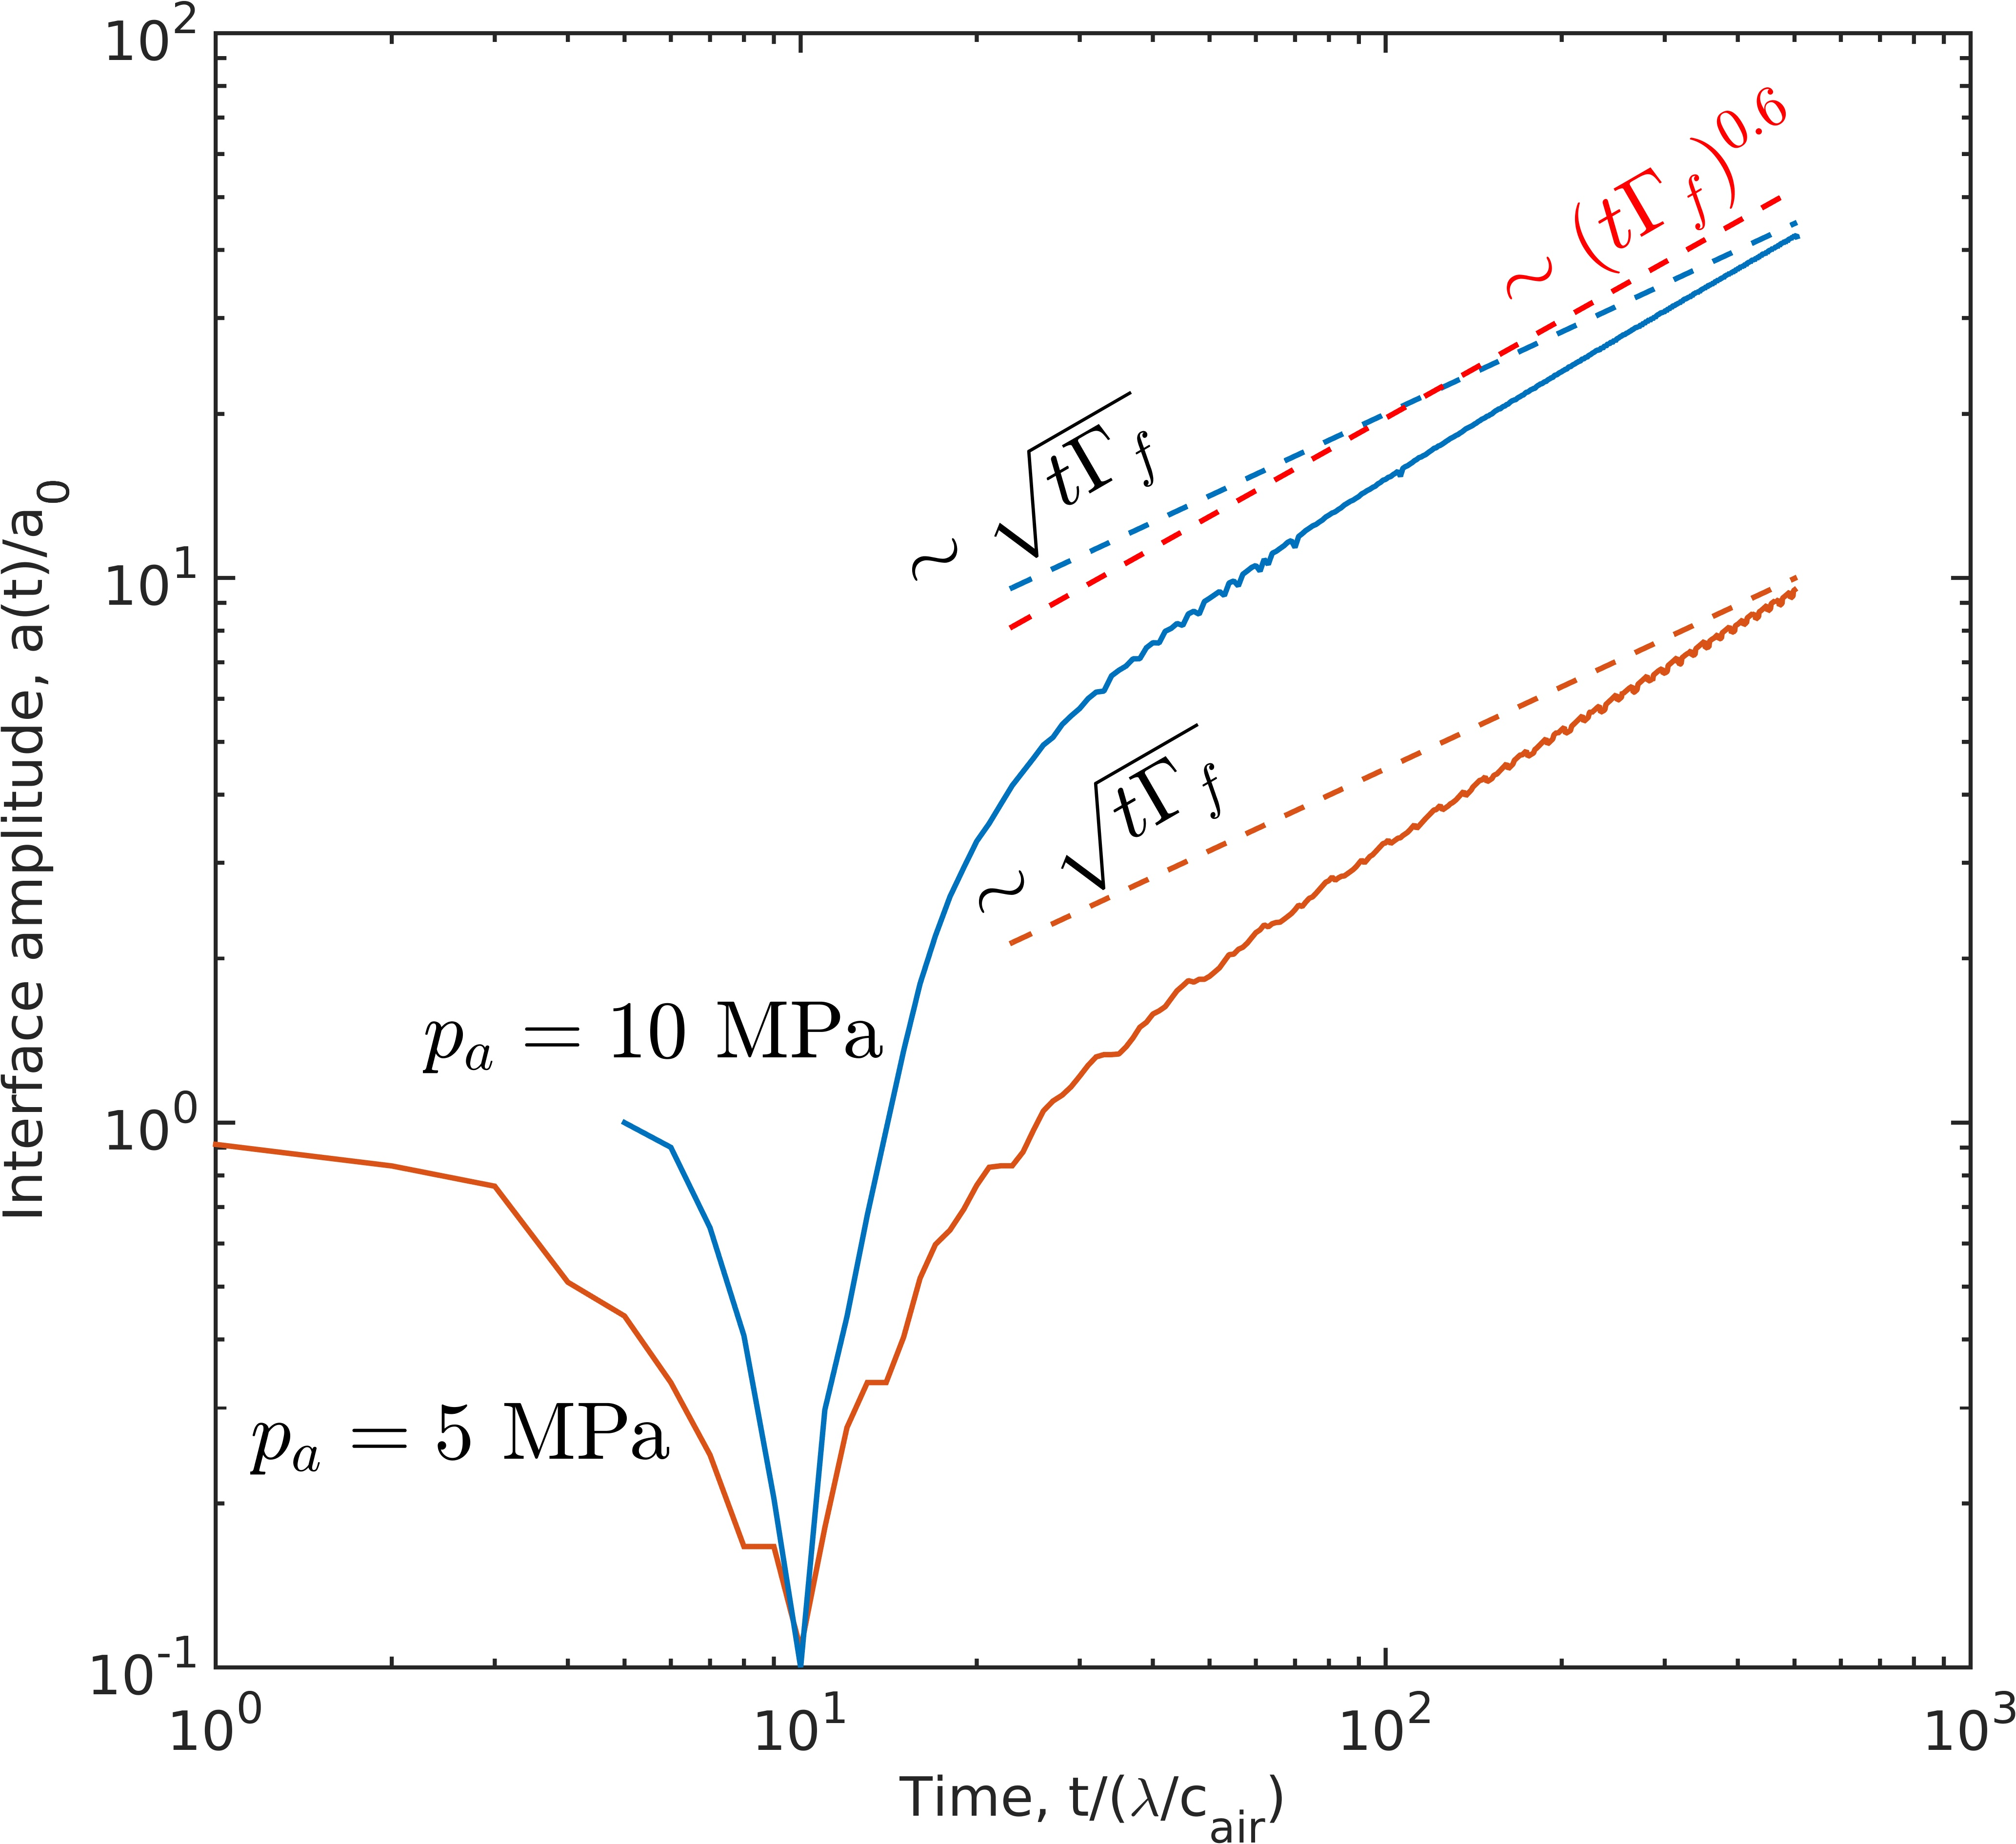
\includegraphics[width=0.48\textwidth]{./figs/lung_figs/interface_multi-amp_loglog_roe_extra}
%   \includegraphics[width=0.48\textwidth]{./figs/lung_figs/circulation_multi-amp2_roe}
%   \caption[The interface and circulation dependence on wave amplitude
%   at long time]{The interface amplitude (left) and circulation (right)
%     histories corresponding to the $5$(orange) and $10$(blue) MPa
%     trapezoidal waves are shown for $t\leq 500$. To appropriately
%     compare late time dynamics, time has been offset in the interface
%     amplitude history such that the phase reversal appears to occur
%     simultaneously in both simulations. Dashed lines of the same color
%     are used to demonstrate the expected slope of pure circulation
%     driven interface growth, based on Equation
%     \eqref{eq:intf_circ_scaling}. The red dashed line shows the slope we
%     appear to be approaching for the $10$ MPa wave case for the end time.}
%   \label{fig:trapz_circ_interface_loglog}
% \end{figure}
% %
% \subsubsection{Circulation and vorticity dynamics}
% We observe that the wave deposits a sheet of vorticity along the
% interface that moves with the interface in time. Figure
% \ref{fig:trapz_ddt_circ} shows a surface plot of vorticity in the
% region of the domain around the interface for the $10$ Mpa trapezoidal
% wave case, at $t=0.6$, during the middle of the interface-compression
% wave interaction (Left). Not shown is the rest of the domain, where
% vorticity was relatively insignificant. The vorticity is antisymmetric
% across the $x=0.5$ center line. To analyze the physical mechanisms
% generating the vorticity, we plot each term of the circulation
% generation equation \eqref{eq:circulation_generation} during the
% period around the compression wave-interface interaction. Near the end
% of the interaction at $t=1.0$,
% $\left(\partial \Gamma/\partial t\right)_{advective} =
% 5.3\,\text{e}{-5}$; %
% $\left(\partial \Gamma/\partial t\right)_{compressible} =
% -2.7\,\text{e}{-5}$; %
% $\left(\partial \Gamma/\partial t\right)_{baroclinic} =
% -7.7\,\text{e}{-3}$; %
% $\left(\partial \Gamma/\partial t\right)_{total} =
% -7.7\,\text{e}{-3}$. %
% This result is quantitatively consistent with expected vorticity generation
% based on our analysis \eqref{eq:vorticity_comparison}. Furthermore, it
% supports our hypothesis that vorticity is primarily baroclinically
% generated. 
% %
% \begin{figure}[h] 
%   \centering
%   \includegraphics[width=0.35\textwidth]{./figs/lung_figs/vorticity2}
%   \includegraphics[width=0.48\textwidth]{./figs/lung_figs/ddtcirc}
%   \caption[The vorticity field and individual contributions to circulation by physical mechanism]{A surface plot of vorticity for the $10$ MPa trapezoidal
%     wave case, at time $t=0.6$, during the middle of the
%     interface-compression wave interaction (Left). Each term of the
%     circulation generation equation \eqref{eq:circulation_generation} is plotted as a function of time:
%     $\left(d\Gamma/dt\right)_{advective}$ (blue),
%     $\left(d\Gamma/dt\right)_{compressible}$ (orange),
%     $\left(d\Gamma/dt\right)_{baroclinic}$ (yellow),
%     $\left(d\Gamma/dt\right)_{total}$ (purple, dotted) is plotted as a
%     function of time (Right).}
%   \label{fig:trapz_ddt_circ}
% \end{figure}
% %
% \subsubsection{Dependence on time-dependent wave features: time lag between compression and expansion waves}
% To demonstrate the importance of time-dependent wave features, we
% simulate $p_a=10$ MPa trapezoidal waves of varying duration impinging
% onto the water-air interface. The compression and expansion portions
% of the waveform are exactly the same as is in the other trapezoidal
% wave cases, with pressure rising and falling over an initial distance
% of $5\lambda$. We vary the duration of interaction between interface
% and the elevated static pressure portion of the wave, we will consider
% in terms of the static portion of the wave's initial length, defined
% as $\Delta x_{lag}$. We decrease this duration from the typical
% $\Delta x_{lag}=35\lambda$ to
% $\Delta x_{lag}=25\lambda, 20\lambda, 15\lambda, 5\lambda,$ and
% $0\lambda$. For each of these cases the system dynamics are virtually
% identical to the original case until the expansion encounters the
% interface. Figure \ref{fig:trapz_circ_interface_multi-lag} shows the
% interface amplitude and circulation histories for each case. For the
% three longest duration trapezoidal waves, with static elevated
% pressure durations of $\Delta x_{lag}=35\lambda, 25\lambda$ and
% $20\lambda$, we note that the expansion encounters the interface after
% the phase reversal has already occurred. In these cases, the expansion
% deposits additional circulation at the interface. For the shorter
% duration waves, with static elevated pressure durations of
% $\Delta x_{lag}=10\lambda, 5\lambda$ and $0\lambda$, the expansion
% encounters the interface before the phase inversion and the net
% half-domain circulation is decreased. We note that before or after the
% phase change of the interface, the larger $a(t)$ is at the time the
% expansion encounters the interface, the more circulation is generated
% by the wave, though this does not necessarily hold true across the
% phase inversion.
% %
% \begin{figure}[h] 
%   \centering
%   \includegraphics[width=0.48\textwidth]{./figs/lung_figs/interface_multi-lag}
%   \includegraphics[width=0.48\textwidth]{./figs/lung_figs/circulation_multi-lag}
%   \caption[The interface and circulation dependence on wave duration]{The interface amplitude (left) and circulation (right)
%     histories for varying elevated static pressure durations or lag
%     time $\Delta x_{lag}$ between the expansion and compression
%     waves. Here we show results for $\Delta x_{lag}=35\lambda$ (blue),
%     $\Delta x_{lag}=25\lambda$ (orange), $\Delta x_{lag}=20\lambda$
%     (yellow), $\Delta x_{lag}=10\lambda$ (purple),
%     $\Delta x_{lag}=5\lambda$ (green), $\Delta x_{lag}=0\lambda$
%     (light blue)}
%   \label{fig:trapz_circ_interface_multi-lag}
% \end{figure}
% %
% \subsection{Interface response to \acf{DUS} waves}%
% \label{subsec:usbe_lung_trapezoidal_results}%
% To evaluate the relevance of our trapezoidal wave experiments we simulate
% a $p_a=1, 5$ and $10$ MPa \ac{DUS} pulse waves (See Figure
% \ref{fig:p0}) impinging onto the water air interface. In figure
% \ref{fig:us_circ_interface} we illustrate the circulation and
% interface amplitude histories for the $p_a=10$ MPa \ac{DUS} like-pulse
% case. The post-wave interface dynamics are similar to those observed
% for trapezoidal wave cases. During the wave-interface interaction, the
% interface amplitude is compressed overall, but oscillations are
% observed in correspondence with the acoustic pulse oscillations. After
% the wave has left the interface, the perturbation amplitude continues
% to decrease until the interface undergoes a phase inversion, after
% which the perturbation amplitude grows for the remainder of the
% simulation. half-domain circulation oscillates during wave-interface
% interaction before settling to a nearly constant non-zero value after
% the wave has passed. We note that the total circulation deposited is
% of the same order of magnitude as that generated by the trapezoidal
% wave of the same amplitude and duration. Qualitatively similar results
% were observed for the $5$ MPa case. For the one $1$ MPa case, the
% evolution of the system was slow such that running the simulation long
% enough to obtain useful results was computationally prohibitive.

% \begin{figure}
%   \centering
%   \includegraphics[width=0.48\textwidth]{./figs/lung_figs/us_intf_schematic} \hfill
%   \includegraphics[width=0.48\textwidth]{./figs/lung_figs/us_circ_schematic}
%   \caption[The interface amplitude and circulation histories for the \ac{DUS} pulse]{The interface amplitude (left) and circulation (right)
%     histories corresponding to the a water-air interface disturbed by
%     the US-like pulse shown in Figure \ref{fig:p0}.}
%   \label{fig:us_circ_interface}
% \end{figure}

% \subsection{Further discussion of the results}%
% \label{subsec:usbe_lung_further_discussion}%
% For both the trapezoidal and \ac{DUS} pulse acoustic waves, the
% pressure, velocity, and density return to initial, ambient conditions
% after the passing of the wave. As these waveforms are continuous, this
% implies that the integral of the pressure gradient $\nabla p$ at each
% point along the interface, over all time must be zero. Hence we
% surmise that if the interface remains unchanged during the interaction
% with the wave, as it would for a wave moving with infinite velocity,
% $\nabla \rho$ remains constant and the net baroclinic circulation
% deposited must be zero. Thus for any finite duration acoustic wave
% such as ours to deposit net baroclinic circulation upon an interface,
% the interface itself must deform during interaction with the
% wave. This deformation alters the misalignment of the pressure and
% density gradients at the interface causing positive and negative
% circulation deposited to not cancel out entirely. Note that this is
% unique to waves that begin and end at the same pressure. This is not
% the case for the traditional \ac{RMI} problem, for which conditions do
% not return to their original state after the passage of the shock.

% For the cases varying the length of the static elevated pressure in
% the trapezoidal wave we previously noted that whether the expansion
% increased or decreased the total half-domain circulation depended on
% whether it encountered the interface before or after the phase
% change. If indeed circulation is driving the deformation of the
% interface, then changes in the waveform that appear to have very
% little effect on the interface dynamics during the wave-interface
% interaction period, may have far more significant impacts on the long
% term dynamics of the interface. To put this in the context of
% \ac{DUS}, which uses repeated pulses, if ultrasonically-deposited
% circulation is causing deformation within the lungs, longer \acp{PD}
% may allow for greater deformation and increased circulation deposition
% as a result of any individual pulse. If the system acts as we have
% modeled it, the \ac{PRF} would determine the degree of interface
% deformation experienced by pulses subsequent to the first and may
% influence deformation and hemorrhage. Finally, in recognition of the
% limitations of this study, we note that the true physical nature of
% lung tissue is viscoelastic \citep{Bayliss1939}, and neither viscosity
% nor elasticity is included in our model problems. While preliminary
% results with a Navier-Stokes code showed similar early time results,
% we expect that viscosity would dissipate circulation over a long
% enough period of time. Furthermore, elasticity may provide a mechanism
% by which the alveolar walls could resist deformation or retard to
% their original shape between pressure perturbations.




%%% Local Variables:
%%% mode: latex
%%% TeX-master: "../../prelim"
%%% End:

\section{Conclusions}
\label{sec:usbe_lung_conclusions}
This work is unique in that it demonstrates that acoustic waves may
trigger significant deformation of perturbed liquid-gas interfaces
over long periods of time. The driving mechanism behind this
deformation is baroclinic vorticity, which occurs as a result of
misalignment between the pressure gradient of the acoustic wave and
density gradient of the perturbed interface. This mechanism arises as
a result of nonlinear, compressible fluid mechanics, and cannot be
predicted through traditional linear acoustics. We suggest that
nonlinear effects such as baroclinic vorticity are important at
liquid-gas interfaces, such as those in the lungs, because of the
sharp density discontinuities between air and tissue within the
lungs. To demonstrate this we simulate acoustic waves with properties
relevant to \ac{DUS} impinging from water into air.

The work presented here supports the following three conclusions:%
%
(1) Baroclinic vorticity generated by acoustic waves within the
\ac{DUS} regime is capable of significantly deforming perturbed
liquid-gas interfaces. We observed that much of the vorticity
generated by the acoustic wave at the interface remains with the
interface as it evolves and deforms even long after the passage of all
acoustic waves. Part of this is attributed to a lack of physical
mechanism for dissipating vorticity in the inviscid case
considered. From dimensional analysis we find scaling law
\eqref{eq:intf_circ_scaling}, suggesting that the interface
perturbation amplitude will grow as $t^{0.5}$ for purely circulation
driven growth. In our computed results we find the actual perturbation
amplitude grows as $t^{0.6}$. This slight discrepancy could be a
result of the inability of a global quantity $\Gamma$ to completely
describe $a(t)$ which is governed by local fluid mechanics.
%
(2) During interactions between acoustic waves and perturbed
liquid-gas interfaces, baroclinic vorticity is predominantly deposited
in the gas-dominated fluid. We perform analysis to predict that on either
side of an infinitely sharp water-air interface, the vorticity
generation rate would be approximately two orders of magnitude greater
on the air side of the interface than in the water. This is
qualitatively supported by our computational results which find that
near the end of the initial compression wave-interface interaction
nearly all of the circulation exists in fluid dominated by air. For
the $10$ MPa wave, for instance, 97\% of the circulation is found in
fluid with volume fraction of water $\alpha<0.5$ at $t=1$, after 91\%
of the compression has passed.
%
(3) Changes in the acoustic waveform that have little effect on the
interface dynamics during their interaction can substantially effect
the interface over longer periods of time, via vorticity. By comparing
the effects of $10$ MPa trapezoidal waves with varying static pressure
durations between compression and expansion, we observe that the
evolution of the interface between these two wave components
drastically effects the ultimate growth rate of the interface. The
phase and amplitude of the interface perturbation at the time it
encounters the expansion wave determine the direction and magnitude
respectively of the vorticity deposited. Consequently, the amount of
vorticity remaining at the interface and in the surrounding fluid
after the passage of the wave changes greatly based on the
time-dependent features of the wave.

This work is a step toward understanding the effects of acoustically
generated vorticity on gas-liquid interfaces, however we acknowledge
that there are many questions left to be answered. However, we
consider our findings in the context of \ac{DUS}-induced \ac{LH} and
propose a previously unconsidered potential damage mechanism. We
hypothesize that baroclinic torque occurs at fragile air-tissue
interfaces of the lung due to misalignment between the \ac{US}
pressure gradient and material interface density gradient, causing
stress, deformation, and ultimately rupture at the interface. We note
that evaluation of the hypothesized damage mechanism will require
considerable further work including experiments, and at the very
least, numerical simulations that incorporate realistic viscosity,
elasticity, attenuation, and realistic waveforms and lung
geometries. This validation is beyond the scope of the proposed
dissertation.

%%% Local Variables:
%%% mode: latex
%%% TeX-master: "../../prelim"
%%% End:

\section{Future Work} \label{sec:usbe_lung_future}%
Finally, we address some of the limitations of this study and propose
future work to address some of these issues. To further evaluate the
relevance of the proposed damage mechanisms and presented results to
\ac{DUS}-induced lung hemorrhage, viscous and elastic effects should
be considered, as both of these have the potential to reduce observed
deformation, and mitigate hemorrhage. Additionally, geometries that
more accurately represent physical networks of alveoli within the
lungs will be useful to understand the propagation of ultrasound waves
and hemorrhage deeper into the lungs, beyond the first tissue-air
interface. To do this accurately, it may be necessary to include a
model for interface rupture. Many of these future tasks will require
not only numerical efforts, but also experimental studies to
appropriately characterize the lung tissue and validate the suggested
models. Additionally, to increase our understanding of the relevant
fluid dynamics, it would be useful to be able predict the circulation
and interface dynamics based on the wave properties and initial
conditions.

To address some of these issues and complete the proposed dissertation
research we plan to perform several tasks:

\begin{itemize}
\item To further the relevance of this research to the problem of
  \ac{DUS} of the lung we will:
  \begin{enumerate}
  \item Calculate stresses and strains at the interface and compare to
    previously measured failure thresholds of the lungs. A passive
    viscous stress tensor will be computed from the velocity field and
    volume fraction fields, assuming constant viscosity for pure water
    and air. Either Volume fraction fields or Lagrange particles will
    be used to calculate the pathlength of the interface as a function
    of time $S_{Intf}(t)$ and engineering strain of the interface,
    $\varepsilon_{Intf}$, as though the interface were a solid sheet
    of tissue where,
    $\varepsilon_{Intf}=[S_{Intf}(t=0)-S_{Intf}(t)]/S_{Intf}(t=0)$.
    % 
  \item Investigate the effects of alveolar side wall structures. To
    model this, a thin layer of tissue (modeled as water) will be
    placed at the edges of the alveolus (modeled as air) and periodic
    boundary conditions will be used.
    %
  \item Investigate the propagation of ultrasound waves and hemorrhage
    into the lungs. To model this we will modify the current geometry
    to such that a thin sinusoidal strip of water, parallel to the
    initial interface, will be be placed every $\lambda$ deep into the
    alveoli. This will be used with then be used with the alveolar
    walls described above to simulate a diagnostic ultrasound pulse
    propagating into a uniformly distributed alveolar network.
    %
  \end{enumerate}
  % 
\item To further our understanding of fluid mechanics
  associated with acoustically perturbed fluid interfaces we will:
  \begin{enumerate}
  \item Seek to understand discrepancies between the
    $a(t)\sim\sqrt{\Gamma t}$ scaling obtained and the numerical
    results. This may require longer simulations to reach the final
    growth rate of the interface, or re-assessment of the logic behind
    using a global metric to describe a locally-dependent flow
    feature.
    % 
  \item Develop a model to predict the circulation deposited on a
    slightly perturbed interface by a simple compression or expansion
    wave. To do this, we will assume the interface is static during
    the interaction with the wave. Then, estimate the baroclinic term
    of the vorticity equation based on known interface and wave
    properties and linear acoustic relationships between state
    variables.
    %
  \item Develop a model to predict the interface phase-reversal time
    for a simple compression wave. This model will be based on the
    expected compression of the interface due to the rising pressure
    during the interaction with the wave, and the subsequent
    circulation driven deformation described by scaling law
    \eqref{eq:intf_circ_scaling}.
    %
  \item Design acoustic waveforms that utilize time dependent features
    and interface deformation to generate minimal circulation and
    interface growth. To do this, we will will aim to create waves
    that deposit vorticity of opposite sign and approximately equal
    magnitude before and after the interface phase change. One example
    of a wave that will be considered is a single period sinusoidal
    pressure wave that changes from the compression to expansion as
    the phase of the interface inverts.
    %
  \item Investigate the cause of late time circulation growth observed
    in some simulations. As can be seen from the circulation history
    for the $10$ MPa trapezoidal wave in Figure
    \ref{fig:trapz_circ_interface_loglog}, circulation continues to
    grow after all waves have left the domain. We plan to first
    determine if this effect is physical or numerical. If this effect
    is physical, we aim to determine the mechanism.
    %
  \end{enumerate}
\end{itemize}

%\hl{FUTURE: ESTIMATE a0 THAT WOULD MAKE BAROCLINIC CIRCULATION EQUAL TO OTHER TERMS TO FIGURE OUT HOW LARGE a0 MUST BE TO GET RM}





% \begin{comment} Move this stuff to introduction There has been a
%   significant amount of prior research into ultrasound-induced
%   pulmonary hemorrhage, but in spite of this there are still many
%   questions left unanswered.  Presently the underlying damage
%   mechanism causing the hemorrhage is not currently known.  Research
%   has shown that the underlying mechanism of US-induced pulmonary
%   hemorrhage is non-thermal. \citet{Zachary2006a}, for instance,
%   compared lesions generated with DUS to those generated via laser
%   and found multiple differences in the injured tissue. Other
%   studies have shown that inertial cavitation, the intially
%   suspected mechanism, is also unlikely to be responsible for the
%   US-induced PH. \citet{Raeman1997} injected the UCA Albunex, which
%   is expected to nucleate cavitation when exposed to US, into mice
%   before performing pulmonarry US and showed that the hemorrhage was
%   similar to that observed in control mice injected with saline.  In
%   a later study \citet{Obrien2000} placed mice under increased
%   hydrostatic pressure, to suppress the occurence of inertial
%   cavitation, before exposure to pulmonarry US, and found that
%   hemorrohage was enhanced by the increased pressure. While it is
%   widely suspected that the cause of the hemorrhage is mechanical,
%   the precise underlying mechanism by which acoustic energy is
%   tranduced into mechanical stress and strain in the capillary has
%   remained elusive.

%   We hypothesize that sharp pressure gradients in the US wave
%   interact with the strong density gradients at the blood-air
%   barriers in the lungs, in turn generating baroclinic vorticity at
%   the interface between the alveoli and the adjacent capillary
%   sheets.  Furthermore, we propose that this vorticity drives the
%   growth of this interface, causing strain, stress, and ultimately
%   failure.
% \end{comment}


% The future work investigating ultrasound-induced pulmonarry
% hemorrhage will be divided into two tasks.  First, further numerical
% simulations of liquid-gas interfaces with pressure waves will be
% performed in order to investigate US-generated baroclinic vorticity
% in the lung as a possible mechanism for hemorrhage. Second a
% simplified model of ultrasound propagation into the lung will be
% created.

% \section{Numerical investigation of ultrasound-lung interaction}
% To investigate the behavior of tissue-air interfaces with DUS waves,
% the lung will be modeled as a compressible fluid system.  As in the
% prior work, the alveoli will be modeled as air. The surrounding
% tissue will be treated as a Newtonian fluid with the density and
% viscosity of blood and all other relevant properties will be set to
% those of water. The liquid-gas interface will be modeled as a
% sinusoid of wavelength $\lambda=200\mu$m, as is consistent with
% typical alvelolar diameter (ADD CITATION). A series of simulations
% will be performed in which this liquid-gas interface will be
% subjected to a pressure waveforms of increasing complexity.

% \section{Baroclinic vorticity generation at the alveolar-capillary sheet interface blood-air barrier}
% \subsection{Estimations of vorticity generation}
% \subsection{Expected interface growth from vorticity at the
% interface }

% \section{Simulations of acoustic wave interactions with a sinusoidal blood-air interface}
% \begin{itemize}
% \item Proposed experiment 1: Interaction of a sinusoidal blood-air interface with a planar acoustic wave with linearly-increasing amplitude
% \item Proposed experiment 2: Interaction of a sinusoidal blood-air interface with a sinudoidal pressure pulse
% \item Proposed experiment 3: Interaction of a sinusoidal blood-air interface with a single DUS pulse
% \item Proposed experiment 4: Interaction of a sinusoidal blood-air interface with multiple DUS pulses
% Space pulses based on accepted experimental procedure and see how the secondary pulses effect the interaface growth.
% \end{itemize}

% \section{Modeling US propagation into the lung}
% I aim to model the propagation of ultrasound waves into the lungs.  Much of the lung is composed of tiny air-filled sacs called alveoli. Due to the large impedance mismatch between these alveoli and their surrounding tissue, the lung is highy acoustically reflective.

% \subsection{Propogation of acoustic energy into the lung}
% Use linear acoustics to predict the transmitted and reflected acoustic pressure amplitudes for air pockets separated by thin water (blood) membranes.  (1a) Model adjacent alveoli as first as normal planar slabs of air with thickness equal to alveolar diameter ($200\mu$m), seperated by slabs of water (blood) of alveolar membrane diameter ($1\mu$m).  (1b) Then model packed regular triangles, (1c) squares (faces oriented at π/4 relative to incoming plane wave.


%%% Local Variables:
%%% mode: latex
%%% TeX-master: "../../prelim"
%%% End:

%\section{abstract}
  Diagnostic ultrasound has been shown to cause lung hemorrhage in a
  variety of mammals, though the underlying damage mechanisms are
  still unclear. Motivated by this problem, we use numerical
  simulations to investigate the interaction of an ultrasound wave
  with the alveolar tissue-air interface. A planar trapezoidal waveform
  propagates in tissue (modelled as water) and
  impinges upon an alveolus of the lung (modelled as air); to
  represent the alveolar surface roughness, the interface consists of a
  small-amplitude, single-mode perturbation. Because of the sharp
  density gradient at the interface, we hypothesize that ultrasound
  waves, despite their relatively low amplitude, deposit sufficient
  baroclinic vorticity to drive perturbation growth. Our simulations
  show that the perturbation amplitude grows to sizes many times
  larger than the original value, \emph{well after the wave has
    passed}. We demonstrate that conventional (linear) acoustics
  cannot account for such deformations; instead, the perturbation
  growth is driven by nonlinear effects---the baroclinic vorticity
  deposited along the interface, due to the misalignment of the
  pressure gradient (across the wave) and the density gradient (across
  the perturbed gas-liquid interface). Based on dimensional analysis
  and scaling we observe that the amplitude and length of the
  interface scale with the circulation density and grow according to
  power laws in time. If the interval between the pressure increase
  and decrease is sufficient, both deposit vorticity of the same sign,
  thus enhancing the perturbation growth; conversely, if the interval
  is too short, the vorticity deposited by the pressure increase is
  canceled by the decrease. A further consequence is that one may be
  able to control the growth of such perturbed interfaces by
  modulating the incoming wave.

\section{Introduction}%
\label{sec:introduction}%
\ac{DUS} is one of the safest forms of medical imaging and has become
ubiquitous in clinical practice. \ac{DUS}-induced lung hemorrhage is
the only known bioeffect of non-contrast, pulsed \ac{US}, as bleeding
has been shown to occur in mammals including mice, rats, rabbits,
pigs and monkeys
\citep{Child1990,OBrien2006a,Tarantal1994a,Miller2012}.  Furthermore,
this problem has been shown to occur for a wide range of frequencies
ranging $1.5-12$ MHz for Mechanical indices well below the accepted
safe limit for diagnostic ultrasound, $\mbox{MI}=1.9$. Although this problem
does not appear to be of medical safety concern for humans under
typical conditions, there is a need to better understand the physical
mechanisms of \ac{DUS}-induced lung hemorrhage.
Well-established \ac{US} bioeffects do not readily explain \ac{DUS}-induced
lung hemorrhage. \ac{US} bioeffects mechanisms are generally
classified as thermal or non-thermal, with the bulk of non-thermal
bioeffects being a result of acoustically driven inertial
cavitation. Except for one study reporting cavitation activity
\citep{Holland1996}, the bulk of research on hemorrhage mechanism
suggests that inertial cavitation is not the cause of \ac{DUS}-induced
lung hemorrhage: \cite{Raeman1996} and \cite{OBrien2004} found that
bleeding is not worsened by the use of ultrasound contrast agents,
and \cite{OBrien2000} observed that the severity of the hemorrhage
increases when the hydrostatic pressure is raised.
Beyond lung hemorrhage, a number of studies have explored nonlinear mechanisms as a potential
cause for bioeffects. \cite{Filonenko2001} developed numerical models
to study the effects of acoustic nonlinearity on wave propagation and
heating in soft tissue. \cite{Khokhlova2006} numerically solved a
KZK-type equation simulating the \ac{HIFU} field in a tissue phantom
with the purpose of studying the impact of nonlinear propagation,
cavitation and boiling on lesion formation. Based on potential flow
simulations of an inviscid free surface subjected to a Gaussian
velocity potential, \cite{Tjan2007} suggested another damage mechanism
for \ac{DUS}-induced lung hemorrhage, namely that under the right circumstances focused \ac{US} may
lead to the ejection of droplets capable of puncturing the air-filled
sacs within the lung. \cite{Simon2012}
experimentally demonstrated atomization of water and soft tissue at
air interfaces exposed to 2 MHz \ac{HIFU} though at amplitudes higher than diagnostic. Despite these efforts, the precise
damage mechanism underlying \ac{DUS}-induced lung hemorrhage is still
unknown.

In parallel, the dynamics of accelerated interfaces between fluids of different densities have
been the subject of intensive studies in fluid mechanics. When exposed
to accelerations whose sign is opposite that of the density gradient,
interfacial perturbations grow exponentially as a manifestation of the
Rayleigh-Taylor (RT) instability \citep{Taylor1950}. Bubbles of light fluids ``rise'' into the
heavy fluid while spikes of heavy fluid ``fall'' into the light
fluid. Although the original analysis pertained to perturbation growth
at early times under constant acceleration, extensions to nonlinear
growth and time varying accelerations have been performed. In the
limit of instantaneous acceleration (e.g., as produced by a shock
wave), perturbations grow linearly in time, as predicted by
Richtmyer-Meshkov (RM) analysis \citep{Richtmyer1960, Meshkov1969},
regardless of the sign of the density gradient. \cite{Hecht1994}
developed a potential flow model for both RT and RM flows with Atwood
Number
$A=\frac{\rho_{heavy}-\rho_{light}}{\rho_{heavy}+\rho_{light}}=1$,
which describes bubble growth in both linear and nonlinear
regimes. \cite{Srebro2003} presented a buoyancy-drag model to describe
the perturbation growth for time-dependent Atwood number and
acceleration profile. In both RT and RM
flows, perturbation growth can be explained by vorticity generated
baroclinically, i.e., due to the misalignment of the density and
pressure gradients:
\begin{align}
  \label{eq:baroclinic_equation}
  \frac{d\omega}{dt} \biggr\rvert_{baroclinic} = \frac{\nabla \rho \times \nabla p}{\rho^2}.%
\end{align}
The majority of RT research has examined interfacial perturbation
growth under constant acceleration fields; RM research is primarily
concerned with shock-accelerated interfaces, where the
post-shock pressure is kept raised \citep{Brouillette2002}. There has been
limited study of transiently accelerated fluid
interfaces. \cite{Mikaelian1996} simulated shock passage through
multiple gas layers with sinusoidally perturbed interfaces to show
that subsequent reshock by reflected waves causes the flow to evolve
into a complex nested mushroom morphology. \cite{Mikaelian2009}
developed a model for hydrodynamic instabilities driven by
time-dependent accelerations, which agreed well with full
simulations. \cite{HenrydeFrahan2015b} demonstrated that subsequent
interactions between reflected and transmitted
shocks and rarefactions with interfaces in layered media could be used to decrease and
possibly control the long term growth of a shock-accelerated
interface.
Much of the past research in both RT and RM flows has
focused largely on gas-gas interfaces. \cite{Haas1987} experimentally
shocked helium and R22-filled bubbles in air. They showed that
transmitted waves overtake one another and merge downstream as a
result of nonlinear gas dynamics. Numerical simulations of
shock-bubble interactions have verified the timescales and physical
features observed in these experiments. These simulations, in
conjunction with nonlinear theory, have shown that baroclinic
vorticity is generated by the wave-interface interaction, and
dominates the late-time dynamics of the system
\citep{Picone1988,Quirk1996}.

% \hl{(buoyancy-drag and time varying references here, see  Eric's comment)}

We submit that an ultrasound wave propagating in tissue and impinging
upon the lung may give rise to perturbation growth along the
interface, much like that observed in RT and RM flows. Despite being
smooth by contrast to shocks, ultrasound waves in tissue have pressure
amplitudes on the order of megapascals over millimeters; although the
strength of the waves is relatively small given the large density and
sound speed, the pressure gradients are non-negligible. Furthermore,
the density jumps by several orders of magnitude over a few microns
across the tissue-air interface. These observations motivate our
hypothesis, namely that baroclinic vorticity generated by the
misalignment of the pressure gradient across the ultrasound wave and
the density gradient across the tissue-lung interface causes
interfacial perturbations to grow, even after the passage of the
wave. Such a phenomenon cannot be described by linear
acoustics. Ultimately, if the growth is sufficient over the relevant
time scales, capillary rupture may follow. However, the fluid
mechanics of this process are expected to be different from classical
RT and RM theory: by contrast to conventional RT analysis, the
acceleration imparted by the pressure wave is time-varying and
transient; as opposed to the classical RM process, the transient wave
deposits vorticity over a finite duration. Thus, the transient nature
of the problem (e.g., interface deformation during wave interaction)
is expected to be important.  Our objective is to predict the growth
of perturbations along water-air interfaces subjected to time-varying
pressure waves using numerical simulations, under conditions relevant
to diagnostic ultrasound. To probe the basic mechanics, the
tissue-lung interface is modeled as a water-air interface, and the
ultrasound waveform is idealized to a trapezoidal wave. The article is
organized as follows. We first describe the problem under
consideration and our methods. We then investigate the perturbation
growth and vorticity dynamics of our baseline case. As we seek to
understand the late-time growth, we then examine how the wave
properties (amplitude and length) affect the dynamics. Finally we
summarize the main conclusions and suggest the next steps to be taken.


% =========================METHODS====================================
\section{Fluid mechanics modeling of ultrasound-lung interaction}%
\label{sec:methods}%
%\subsection{}
%\label{subsec:physical_problem}

Consider a diagnostic ultrasound (DUS) pulse traveling into the
lung. Since past studies have observed lung hemorrhage with
frequencies ranging from $1.5-12$ MHz and pressure amplitudes ranging
from $1-12.3$ MPa
\citep{Penney1993a,Child1990,OBrien2000b,Miller2015a}, we consider
pulses in the MHz and MPa ranges.  The wave traverses several layers
of soft tissue and fluid making up the thoracic wall ($\sim 2$ cm
thick) and pulmonary pleura ($\sim 1$ mm thick), whose acoustic
properties (density and sound speed) are close to that of water
\citep{McLean2011}.  The size of the focal region is on the order of
the ultrasonic wavelength $\lambda$, approximately $1$ mm for a $1.5$
MHz wave in tissue.  After passing through the pleurae, the wave
encounters a network of openly connected, air-filled saccules with
distinctly irregular surfaces---the alveoli, whose typical size in
adult humans is $\ell\approx200$ $\mu$m \citep{Ochs2004}.  The lung is
a complex organ, as exemplified by the range of length scales and
physical properties \cite[multiphase, viscoelastic, surface tension,
high gas volume fraction][]{Bayliss1939, Suki1994}.  However,
dimensional arguments suggest that at sufficiently early times
inertial effects dominate in the interaction of an ultrasound wave
with the lung; viscous, surface tension and elastic effects are
negligible. By the end of the simulations considered here, the viscous
boundary layer thickness is approximately
$\sqrt{\nu_{water} t_{final}}\approx 20$ $\mu$m, far less than both a
typical alveolar diameter and the $400 \mu$m amplitudes achieved at
that time in our baseline case.  The Weber number corresponding to the
lung surface tension \cite[ $\sim 9$ mN/m][]{Schurch1976} and a
pressure amplitude of 1 MPa is
$We=p_a\ell/\sigma_{lung}=\orderof{10^4}\gg1$. For an elastic modulus
$K = 5$ kPa \citep{Cavalcante2005}, the acoustic Cauchy number is
$Ca=p_a/K=\orderof{10^2}\gg1$.

Our interest lies in the interaction between an incident ultrasound
cycle and the first alveolar tissue-air interface it encounters, as
illustrated in figure \ref{fig:schematics}.  Given the complexity of
the full problem, we simplify it to a tractable one on the basis of
the above observations. Since viscous, surface tension and elastic
effects are negligible, the dominant mechanics are the wave
propagation, its interaction with the tissue-lung interface and
subsequent interfacial deformations. Thus, we model the thoracic wall
and pleura as water, and the lung as air; both substances are
compressible, with appropriate density and sound speed.  To simplify
the representation of the alveolar surface roughness, the interface is
initially represented by a single-mode sinusoidal perturbation of
amplitude $a_0$,
\begin{align}
  y_{interface}(x,t=0) = a_0\sin\left(\frac{2\pi x}{\ell}-\frac{\pi}{2}\right),
\end{align}
where $a_0=0.03\ell$.  We define the time-dependent interfacial
perturbation amplitude $a(t)$ as half the peak-to-trough distance in
the $y-$direction. On the scale of an alveolus, the incoming wave is
planar.  More complex, corrugated interfaces can be described by
combining such sinusoidal perturbations of varying amplitudes and
wavelengths.  Despite the three-dimensional geometry of the real
problem, we believe that the key physics are well represented by this
two-dimensional description of the interface.


% 
\begin{figure}
  \centering
  \begin{subfigure}[b]{0.48\textwidth}
    \phantomcaption
    \centering
    \def\svgwidth{\textwidth}
%    \import{./figs/lung_figs/}{Alveolus_US_zoom_only_diagram.pdf_tex} \hfill%
    \import{./figs/lung_figs/}{Alveolus_US_tissue_diagram_20170915.pdf_tex} \hfill%
    \label{fig:alveolar_schematic}% Physical problem of interest: an \ac{US} wave impinges upon an alveolus.}
  \end{subfigure}
  ~
  \begin{subfigure}[b]{0.48\textwidth}
    \centering
    \phantomcaption
    \def\svgwidth{\textwidth}
    %\import{./figs/lung_figs/}{usbe_model_schematic_domain.pdf_tex} \hfill%
    \import{./figs/lung_figs/}{usbe_model_schematic_interface_20170915.pdf_tex} \hfill%
    \label{fig:problem_schematic}% A schematic of the domain and model problem.}
  \end{subfigure}
  % 
  \caption[Schematic view of the physical and model problems]{Left:
    Schematic description of the physical problem of interest
    (ultrasound pulse in tissue impinging upon the first alveolus it
    encounters). Right: Computational set-up of the model problem
    (acoustic wave in water impinging upon a sinusoidally perturbed
    air interface of initial amplitude $a_0$).}
  \label{fig:schematics}
\end{figure}
% 


Although our motivation is rooted in \ac{DUS} of the lung, a typical
\ac{DUS} pulse bears challenges when investigating the fundamental
mechanics of acoustically driven perturbed liquid-air interfaces. For
instance, the waveforms are often noisy, continuously vary and come in
as pulses consisting of several cycles of variable amplitude.  For
simplicity, we construct an idealized waveform comprising the
essential elements of \ac{DUS} pulses, as illustrated in figure
\ref{fig:p0}.  By contrast to shock waves, which instantaneously and
impulsively accelerate the interface and maintain a state of high
pressure after their passage, an ultrasound wave continuously
interacts with the interface over the finite duration of its passage;
the pressure returns to its initially unperturbed ambient value
thereafter. Direct application of Richtmyer-Meshkov analysis to relate
the continuously varying pressure profile to baroclinic vorticity
deposition is thus not straightforward. For this reason, we consider a
single, positive trapezoidal wave of amplitude and length relevant to
\ac{DUS}, consisting of a linear pressure increase followed by a
constant elevated pressure, itself followed by a linear pressure
decrease back to ambient. Noting that its intensity is approximately
trapezoidal, the complex, multi-cycle \ac{DUS} pulse is simplified to
a waveform to which Richtmyer-Meshkov-type analysis can be applied:
though finite duration, the pressure gradients are constant and the
time intervals over which vorticity is deposited (pressure
increase/decrease) are clearly defined. Despite this specific choice
for the waveform, we explain in \S \ref{sec:conclusions} how these results
are generalizable to arbitrary waveforms with positive and negative
pressure contributions.

\begin{figure}% 
  \centering%
  \begin{subfigure}[b]{\textwidth}
    \centering
    \def\svgwidth{\textwidth}%
    \import{./figs/lung_figs/}{shock-us_2_trapz_labels_logic.pdf_tex}%
  \end{subfigure}
  \caption[Trapezoidal wave]{Ideological progression from ultrasound
    pulse and shock to a trapezoidal wave that can be analyzed with
    Richtmyer-Meshkov-type analysis.}%
  \label{fig:p0}
\end{figure}

The amplitude and length of the wave are chosen to be relevant to
\ac{DUS}.  The pressure increases from atmospheric by amplitude
$p_a=5.0-12.5$ MPa over a distance $\Delta L_a = 1$ mm for an alveolus
of diameter $200$ $\mu$m.  The wave is symmetric in time such that the
pressure decreases over the same $\Delta L_a$. To keep the pulse
duration consistent with DUS, we choose as a baseline a total pulse
length of $45\ell$ corresponding to 9 mm in soft tissue, or a $5.5$
$\mu$s pulse duration, in the range relevant to previous research
\citep{Child1990,OBrien2006b}. Thus, the length of the constant
elevated pressure is $35\ell$. As such, the initial pressure waveform
is prescribed as
\begin{align}
  \label{eq:p0}
  p(y_f,t=0) = p_{atm} + p_a %
    \begin{cases}
      0,&y_f\leq0 ,\quad$or$\quad y_f\geq45\ell,\\%
      \frac{y_f}{5\ell},&0\leq y_f\leq5\ell,\\%
      1,&5\ell\leq y_f\leq40\ell,\\%
      1-\frac{y_f-40\ell}{5\ell},\qquad\qquad\qquad&40\ell\leq y_f\leq45\ell,%
  \end{cases}%
\end{align}
where $y_f$ is the initial location of the wavefront, here kept as a
constant $a_0+0.3\ell$. At these amplitudes and frequencies, linear
acoustics describes ultrasound propagation in homogeneous tissue, such
that the initial velocity is set to $u=0$ and
$v=0-\Delta p_a / (\rho c)$ and initial density is
$\rho_{water} + \Delta p_a / c^2$ \cite{Anderson1990}, where
$\Delta p_a$ is the acoustic perturbation pressure. The domain size is
sufficiently large to fit the entire initial wave and the deforming
interface.


Once the ultrasound reaches the interface, the pressure differential
(due to the geometrical perturbation) over a short distance along the
sharp interface applies a torque on fluid particles along the interface,
thus generating rotation (or baroclinic vorticity). Since this effect
is nonlinear, linear acoustics cannot account for the vorticity
generated by the interaction of the wave with the interface. For this
reason, we solve the the Euler equations, in two dimensions ($x,y$):
\begin{subequations} \label{eq:euler}%
  \begin{align}% 
    \frac{\partial \rho}{\partial t} + \frac{\partial}{\partial x}\left(\rho u\right) + \frac{\partial}{\partial y}\left(\rho v\right) = 0,\\
    \frac{\partial}{\partial t}\left(\rho u\right) + \frac{\partial}{\partial x}\left( \rho u^2+p\right)  + \frac{\partial}{\partial y}\left( \rho uv\right) = 0,\\
    \frac{\partial}{\partial t}\left(\rho v\right) + \frac{\partial}{\partial x}\left( \rho uv\right)  + \frac{\partial}{\partial y}\left( \rho v^2+p\right) = 0,\\
    \frac{\partial E}{\partial t} + \frac{\partial}{\partial x}\left(u\left[E+p\right]\right) + \frac{\partial}{\partial y}\left(v\left[E+p\right]\right) = 0,
  \end{align}%
\end{subequations}%
where $t$ is time, $\rho$ density, $p$ pressure, $u$ and $v$ the $x-$
and $y-$velocity components and $E$ the total energy. We use a
stiffened equation of state to relate the pressure to the internal
energy,
% 
\begin{align} \label{eq:stiffened_eos}%
  E=\frac{\rho\left(u^2+v^2\right)}{2} + \frac{p+n B}{n-1},
\end{align}
% 
where $B$ is an empirically determined measure of liquid
stiffness. For perfect gases, such as in our treatment of air, $n$ is
the specific heats ratio and $B=0$.

The interface evolution is captured using a $\gamma-$based
\citep{Shyue1998}, such that
\begin{subequations} \label{usbe_lung_eosvar_advection}%
  \begin{align}% 
    \frac{\partial}{\partial t}\left(\frac{1}{n-1}\right)+u\frac{\partial}{\partial x}\left(\frac{1}{n-1}\right)+v\frac{\partial}{\partial y}\left(\frac{1}{n-1}\right) = 0,\\
    \frac{\partial}{\partial t}\left(\frac{n B}{n-1}\right)+u\frac{\partial}{\partial x}\left(\frac{n B}{n-1}\right)+v\frac{\partial}{\partial y}\left(\frac{n B}{n-1}\right) = 0.
  \end{align}%
\end{subequations}%
We initially prescribe a small, finite thickness parameter $\delta$ to
the interface \citep{Latini2007}, such that the initial volume
fraction field is
\begin{align}
  \alpha_0 = %
  \begin{cases}
    1&$\text(water)$,\\%
    \exp\left(\log\left(10^{-16}\right)\abs{d}^8\right)&$\text(mixture)$,\\%
    0&$\text(air)$,%
  \end{cases} \qquad d = \frac{\delta +y_{interface}(x) -y}{2\delta},
\end{align}
where $\delta=0.08\ell$.

The dimensional fluid properties used for air are determined at $300$
K and $1$ atm such that $\rho_{air}=1.18$ kg/m$^3$ and $c_{air}=347.2$
m/s. For water, $\rho_{water}=996$ kg/m$^3$ and $c_{water}=1648.7$
m/s.  The parameters in the stiffened equation of state are
$n_{air}=1.4$, $B_{air} = 0$, $n_{water}=5.5$, and $B_{water} \approx
492$ MPa \citep{Marsh1980,holian1984t,Cocchi1996}. The density and
sound speed of water, as well as the alveolar diameter are used for
non-dimensionalization.

The equations are solved on a domain ranging in the $xy-$plane from
$0 \leq x \leq 1\ell$ (periodic in $x$) and
$-20\ell \leq y \leq 60\ell$ (outflow boundary conditions in $y$). The
$y-$length of the domain is chosen such that the entire wave fits in
the domain initially.  We use a third-order accurate \ac{DG} scheme
($p=1$) in space with the Roe solver and a fourth-order accurate,
adaptive Runge-Kutta method to march forward in time
\citep{HenrydeFrahan2015}. To isolate the effects of a single pulse,
the longest time span reasonable to observe the evolution of the
system of is the time between consecutive pulses, which for a typical
pulse repetition frequency of $1$ kHz is
$t<\delta t_{pulse}=1000 \mu$s \citep{OBrien2000b}. The grid
resolution is 100 points per $\ell$ in $x$ and $y$, except for the top
and bottom-most $10\ell$ segments of the domain, where the grid is
stretched geometrically to minimize artificial reflections. Given the
exceedingly long time duration, we used the highest possible grid
resolution based on our computing resources and time constraints.
Though the solution cannot be fully converged in a pointwise sense
with the Euler equations, the results do show some grid dependence in
certain integral quantities. Nevertheless, the conclusions made on the
basis of our results are still expected to hold.

In this study, we determine the dependence of the time-evolution of
the interfacial amplitude perturbation on the amplitude $p_a$ and
length $L_a$ of the wave. To remain clinically relevant, we consider
amplitudes between $5.0-12.5$ MPa and lengths between $L_a =
10-45\ell$, with our baseline case $p_a=10$ MPa and $L_a=45 \ell$. As
our results will show, this baseline is convenient because the pulse
amplitude is sufficiently strong to evolve the dynamics to late time
within a computationally feasible time, yet not so strong as to drive
the system to behave qualitatively differently than weaker waves
within the diagnostic ultrasound regime.

%============================== RESULTS AND ANALYSIS ================
\section{Results and discussion}%
\label{sec:results}%
 

\subsection{Dynamics of the baseline case}

\label{subsec:Qualitative}
\subsubsection{Density-based description of the perturbation growth}

To exemplify the growth of a perturbation along a water-air interface
driven by the trapezoidal wave of interest, figure
\ref{fig:interface_snapshots} shows the time evolution of density
field for the baseline case. The wave propagates from water (top) to
air (bottom). Frame 1 shows the interface shortly after it first
encounters the wave at $t=4.75$, near the end of the compression. Upon
interaction with the interface, nearly all of the acoustic energy is
reflected back into the water as a rarefaction due to the lower
acoustic impedance of air. The transmitted wave is weakly focused or
defocused in air, depending on the convex or concave nature of the
curved interface. Between frames 1 and 2, the mean interface location
moves in the negative $y$-direction by $0.31$ (corresponding to the
mean acoustic velocity multiplied by the time between the pressure
rise and decrease), advected by the velocity associated with the
elevated pressure. Between these two frames, the perturbation phase
reverses as evidenced by the peak of the perturbation at $x=0.5 \ell$
becoming a valley. From frame 2 on, bubbles of air are observed to
``rise'' into the water along the sides ($x=0, \ell$), while a liquid
spike penetrates the air in the middle ($x=0.5\ell$). This bubble and
spike evolution continues well after the incident wave has passed. The
cumulative effect is that the interface perturbation grows from an
initially smooth sinusoid to a sharp spike at late times.
% 
\begin{figure}
  \centering
  \def\svgwidth{0.95\textwidth}
  \import{./figs/lung_figs/}{snapshots_density_20170727.pdf_tex}
  \caption[The evolution of the acoustically perturbed interface]
          {Density contours at $t=4.75$, 47.5, 475, and 1424 for the
            baseline $p_a = 10$ MPa, $L=45\ell$ trapezoidal
            wave. Black line: $\alpha=0.5$ volume fraction isoline;
            black dashed line: initial interface location.}
  \label{fig:interface_snapshots}
\end{figure}

We turn to a more quantitative description of the time-evolution of
the perturbation in figures \ref{fig:trapz10_interface} (amplitude)
and \ref{fig:trapz10_bs_location} (bubble and spike locations). The
bubble and spike locations are defined as the highest and lowest
$y$-coordinate, respectively, of the constant volume fraction
$\alpha = 0.5$ isoline, and are really meaningful only after phase
reversal; the interface amplitude is calculated by taking the
difference between the bubble and spike locations. The early time
behavior is characterized by several distinct events.  Following the
impingement of the leading end of the wave at $t_1=0.3$, the pressure
at the interface rises until $t_2=5.3$, at which point the pressure
has reached its maximum amplitude.  As the peak of the perturbation
moves in the negative $y$-direction, the interface amplitude decreases
to nearly zero (flat interface) at $t_p=24$, the instant when the
phase reverses.  The amplitude increases thereafter as the initial
peak (now the spike) continues its progress in the negative $y$-direction.
The interfacial pressure remains constant until $t_3=40.3$, at which
point the leading end of the rarefaction reaches the interface. The
pressure decreases until $t_4=46.1$, at which point the full wave has
left the interface and the pressure is atmospheric again, as it was
originally.  The perturbation amplitude continues to grow well after
the wave has passed, reaching many times its initial value. At these
late times, the growth appears to be smooth, continuous and monotonic
in time. This growth may have significant implications in the context
of potential ultrasound-generated damage to the lung as the alveolar
surface elongates, thus potentially rupturing capillaries.

A bit before $t_4$, the slope of the bubble and spike locations
changes significantly, at a time we define as $t_\Gamma=44.6$. We
remark that between $t_2$ and $t_3$ the bubble and spike velocities
consist of the superposition of the wave velocity corresponding to the
elevated pressure and the velocity induced by the baroclinic
vorticity, to be discussed in greater detail in the next section.
Once the magnitude of the former is sufficiently small toward the end
of the passage of the wave, the latter becomes dominant. At this time,
the net bubble velocity becomes positive and rises. This time
$t_\Gamma$, defined as the minimum in the bubble location after phase
reversal, plays an important role in our later analysis.

% 
\begin{figure} 
  \centering
  \begin{subfigure}[b]{0.45\textwidth}
    \centering
    % \includegraphics[width=\textwidth]{./figs/lung_figs/trapz10_intf_schematic.pdf}
    \begin{tikzpicture}%
      \node[anchor=south west,inner sep=0] (image) at (0,0) {
        \includegraphics[width=\textwidth]{./figs/lung_figs/trapz10_intf_schematic_24-May-2017.pdf}
      };%
      \begin{scope}[x={(image.south east)},y={(image.north west)}]%
        %\node[font=\small,right] at (0.85,0.2) {(a)};%
        \node[font=\small,align=center] at (0.0,1.0) {(a)};%
      \end{scope}%  
    \end{tikzpicture}%
    \phantomcaption
    \label{fig:trapz10_interface25}
  \end{subfigure}
  ~
  \begin{subfigure}[b]{0.45\textwidth}
    \centering
    \begin{tikzpicture}%
      \node[anchor=south west,inner sep=0] (image) at (0,0) {
        \includegraphics[width=1.025\textwidth]{./figs/lung_figs/trapz10_intf_t1000_24-May-2017.pdf}%
      };%
      \begin{scope}[x={(image.south east)},y={(image.north west)}]%
%        \node[font=\small,right] at (0.85,0.2) {(b)};%
        \node[font=\small,align=center] at (0.0,1.0) {(b)};%
      \end{scope}%  
    \end{tikzpicture}%
    \phantomcaption
    \label{fig:trapz10_interface1000}
  \end{subfigure}
  \caption[Interface perturbation amplitude history for $p_a = 10$ MPa
    trapezoidal wave]{Interface perturbation amplitude history
    $a(t)/a_0$ for the baseline $p_a = 10$ MPa, $L=45\ell$ trapezoidal
    wave, for $t \leq 120$ \protect\subref{fig:trapz10_interface25}
    and $t \leq 5000$
    \protect\subref{fig:trapz10_interface1000}. In \protect\subref{fig:trapz10_interface25}, times at which
    different stages of the incoming trapezoidal pressure wave first
    encounter the interface are indicated as $t_1$: the compression;
    $t_2$: the constant elevated pressure $p_a$; $t_3$: the rarefaction;
    $t_4$: the return to ambient pressure.}
  \label{fig:trapz10_interface}
\end{figure}\par
% 
%\paragraph{Bubble and spike growth}\\



\begin{figure}
  \centering
  \captionsetup[subfigure]{labelformat=empty}
  \begin{subfigure}[t]{0.45\textwidth}
    \centering
    \includegraphics[height=0.8\textwidth]{./figs/lung_figs/trapz10_bubble-spike_location_15-Sep-2017}
    \caption{Bubble and spike location}
  \end{subfigure}
  \caption{$y$-locations of the bubble and spike for the baseline
    $p_a = 10$ MPa trapezoidal wave case, during and shortly after the
    wave-interface interaction. By definition, the bubble is the top
    (solid, blue) curve and the spike is bottom (red, dashed)
    curve. Black, dotted line: $t_\Gamma$, as defined by the minimum
    bubble location.}
  \label{fig:trapz10_bs_location}
\end{figure}%


The observed evolution of the interfacial perturbation cannot be
explained by linear acoustics.  The combined effects of the
compression and the deformations occurring between the time the wave
travels from the perturbation peak to trough would yield a change in
the amplitude of approximately $0.01 a_0$. Linear acoustics would
further imply that the perturbation should no longer evolve after the
wave passage. The most important contribution of acoustics is the
translation of the interface (downward on the contour plots) during
the interaction with the wave. It follows that nonlinear mechanisms
must drive the perturbation growth.




% As such, non-linear mechanisms are necessary to explain this
% observation, and as we will demonstrate in the upcoming sections, the
% directions of movement of the bubble and spike at $t_\Gamma$ and
% thereafter are consistent with what would be expected if the movement
% was driven by opposing baroclinic vortex pairs deposited by the wave.%
%
% \begin{comment}
%   It is further useful to analyze the growth of the bubble and spike
%   amplitude, as illustrated in for the baseline $p_a = 10$ MPa case
%   in Figure \ref{fig:trapz_bubble-spike_t1000}. Here we define the
%   bubble amplitude $a_b(t)$ and spike amplitude $a_s(t)$ as the
%   maximum and minimum $y-$location of the interface relative to the
%   location of an unperturbed flat interface also driven by the
%   wave. \hl(FIX THIS) The calculated growth of each goes as $t^n$
%   where $n=0.42 ( \text{bubble} ), 0.66 ( \text{spike} )$, and
%   $0.61 ( \text{bubble + spike} )$.%
% \end{comment}
% %
%
% \begin{figure}
%   \centering
%   \begin{subfigure}[t]{0.45\textwidth}
%     \centering
%     \includegraphics[height=0.8\textwidth]{./figs/lung_figs/bubble-spike_t1000_24-May-2017}
%     \caption{\label{fig:trapz_bubble-spike_t1000_unscaled} Constant scaling: $a(t)/\ell$}
%   \end{subfigure}
%   ~
%   \begin{subfigure}[t]{0.45\textwidth}
%     \includegraphics[height=0.8\textwidth]{./figs/lung_figs/bubble-spike_scaled_t1000_24-May-2017}
%     \caption{\label{fig:trapz_bubble-spike_t1000_scaled} Vortex strength scaling: $a(t)/\left(\frac{\Gamma_0}{s_0}\frac{\ell}{c}\right)$}
%   \end{subfigure}
%   \caption{The growth of the bubble (blue), spike (red), and sum of
%     the two (green) are shown for the baseline $p_a = 10$ MPa
%     trapezoidal wave case for $t \leq
%     5000$. \subref{fig:trapz_bubble-spike_t1000_unscaled} shows the
%     amplitudes $a(t)$ scaled by a constant
%     $\ell$. \subref{fig:trapz_bubble-spike_t1000_scaled} shows the
%     interface amplitude after the phase inversion scaled by
%     $\Gamma_0/s_0$, the circulation per unit arc length at
%     $t_\Gamma$. To facilitate the comparison, the time origin has been
%     shifted such that the instant the phase inverts occurs
%     simultaneously in each case. The dashed lines above the curves at
%     late times corresponds to power law growth with time.}
%   \label{fig:trapz_bubble-spike_t1000}
% \end{figure}
%%%%%%%%%%%%%%%%%%%%%%%%%%%%%%%%%%%%%%%%%%%%%%%%%%%%%%%%%%%%%%%%%% 
%%%%%%%%%%%%%%%%%%%%%%%%%%%%%%%%%%%%%%%%%%%%%%%%%%%%%%%%%%%%%%%%%% 
%%%%%%%%%%%%%%%%%%%%%%%%%%%%%%%%%%%%%%%%%%%%%%%%%%%%%%%%%%%%%%%%%% 
%%%%%%%%%%%%%%%%%%%%%%%%%%%%%%%%%%%%%%%%%%%%%%%%%%%%%%%%%%%%%%%%%% 
\subsubsection{Description of the perturbation growth based on vorticity}
\label{subsubsec:vorticity_growth}


The results presented in the previous section demonstrate that the
perturbation amplitude grows well after the incident wave has
traversed the interface, driven by a mechanism that cannot be
explained by conventional linear acoustic analysis.  During
interaction with the interface, the pressure differential (due to the
geometrical perturbation) over a short distance along the sharp
interface applies a torque on fluid particles along the interface,
thus generating rotation (baroclinic vorticity). Such effects are
higher-order for acoustic waves encountering small density variations;
in the present problem however, the pressure and density change over
short distances, thus giving rise to substantial gradients dominating
otherwise first-order (acoustic) effects.  For these reasons, we
examine the perturbation growth in terms of vorticity,
$\boldsymbol{\omega}=\nabla\times\boldsymbol{u}$, whose evolution in
two dimensions is given by
\begin{align} \label{eq:vorticity_euler}
  \frac{\partial \boldsymbol{\omega}}{\partial t}+\left(\boldsymbol{u}\cdot\nabla\right)\boldsymbol{\omega} =% 
  - \boldsymbol{\omega}\left(\nabla\cdot\boldsymbol{u}\right) + \frac{\nabla\rho\times\nabla p}{\rho^2}.%
\end{align}
The high impedance mismatch and relatively low dilation at the wave
amplitudes of interest make the first term on the right-hand side
(dilatation) essentially negligible compared to the last term
(baroclinic) given the nearly discontinuous density gradient and the
significant pressure variations over relatively short lengths;
Appendix \ref{sec:oom_analysis} quantitatively demonstrates that the
vorticity production is baroclinic.  Figure
\ref{fig:vorticity_snapshots} depicts vorticity contours at $t = 4.75,
47.5, 475, 1424$, for the baseline case. Initially, there is no
vorticity in the domain. Frame 1 shows that near the end of the
compression-interface interaction, a vortex sheet exists along the
interface, with negative vorticity between $x/\ell\in[0.0,0.5]$ and
positive vorticity between $x/\ell\in[0.5,1.0]$. The vorticity appears
to be primarily in the air because the interface location (black line)
is defined as the $\alpha=0.5$ isoline. By frame 2, the initially
deposited vorticity has driven the perturbation peak downward such
that the phase is now reversed during the passage of the
rarefaction. Despite the corrugation of the interface, the vorticity
deposited by the rarefaction has the same sign as the distribution
generated by the compression. If the interface had remained
undeformed, the vorticity deposited by the rarefaction would have
canceled that due to the compression.  Instead, the enhanced vorticity
gives rise to a clockwise (left) and counter-clockwise (right) vortex
pair driving the spike to form at $x=0.5\ell$. Over time, the
vorticity contours become fainter.




\begin{figure}
  \centering
  % \includegraphics[width=0.9\textwidth]{./figs/lung_figs/snapshots_vorticity_t1}
  \includegraphics[width=0.98\textwidth]{./figs/lung_figs/vorticity_snapshot_fixcbar_mat_15-Sep-2017}
  \caption[The evolution of the vorticity] {Vorticity contours at $t =
    4.75$, 47.5, 475 and 1424 for the baseline $p_a = 10$ MPa, $L=45
    \ell$ trapezoidal wave case. Black solid line: $\alpha=0.5$ volume
    fraction isoline; black dashed line: initial interface location.}
  \label{fig:vorticity_snapshots}
\end{figure}


During the interface evolution, the vorticity redistributes itself
along the interface. To quantify this behavior, we plot in figure
\ref{fig:vorticity_distribution} the cumulative vorticity (in $y$)
along the interface, $ \int_{-\infty}^{+\infty} \tilde{\omega}(x,y) dy
$, where $\tilde{\omega} = \omega$ for $0 < \alpha < 1$ and is
otherwise $0$ (in pure water or air). Initially, the vorticity is smooth and nearly
sinusoidal, as expected \citep{Samtaney1994}.  During the
phase reversal process, the vorticity peaks move toward
$x=0.5\ell$. Given the geometry at the time when the rarefaction
arrives, a second peak in the vorticity distribution is observed near
$x=0.0$, $1.0\ell$ at $t=47.5$. Though apparently fainter in the
contour plots, the vorticity clearly concentrates near the spike,
driving the heavy fluid into the light one.

\begin{figure}
  \centering
  \includegraphics[width=0.5\textwidth]{./figs/lung_figs/vorticity_distribution_16-Sep-2017}
  \caption{Cumulative vorticity (in $y$) along the interface, $
    \int_{-\infty}^{+\infty} \tilde{\omega}(x,y) dy $, where
    $\tilde{\omega} = \omega$ for $0 < \alpha < 1$ and is otherwise
    $0$ (in pure water or air), at $t=4.75, 47.5, 475$, and $1424$.}
  \label{fig:vorticity_distribution}
\end{figure}


For a more quantitative global measure of vorticity, we consider the
circulation produced in the right-half domain (the left is equal and
opposite by symmetry) for the baseline case in figure
\ref{fig:trapz10_circ_schematic}. The same times at which different
stages of the incoming trapezoidal pressure wave first encounter the
interface are indicated on this figure. From $t_1$ to $t_2$ (during
the interaction of the compression with the interface), positive
vorticity (circulation) is deposited given the geometrical
configuration. This circulation increase is linear since the pressure
and density gradients are constant over the interaction
interval. Other than small changes due to transverse wave reflections,
the circulation remains nearly constant until $t_3$, at which point the
leading edge of the rarefaction encounters the interface. Since the
phase has reversed at $t_p$, the deposited vorticity is of the same
sign (i.e., positive) as that deposited by the compression, such that
the circulation approximately doubles by the time the trailing end of the
rarefaction arrives at $t_4$. Thereafter, any changes in vorticity are
no longer due to the primary incoming wave. The decrease in
circulation observed after the wave passage is due to the interaction
of the transverse reflections of the rarefaction (now compressions)
near the bubble, while the late-time increase is attributed to the
acceleration of the heavy fluid into the light one as the spike
penetrates the air, which is a form of secondary baroclinic vorticity
generation \citep{Peng2003}.

\begin{figure}
  \centering
  \begin{subfigure}[b]{0.48\textwidth}
    \centering
    \begin{tikzpicture}%
      \node[anchor=south west,inner sep=0] (image) at (0,0) {
        \includegraphics[width=\textwidth]{./figs/lung_figs/trapz10_circ_schematic_24-May-2017.pdf}
      };%
      \begin{scope}[x={(image.south east)},y={(image.north west)}]%
        \node[font=\small,align=center] at (0.0,1.0) {(a)};%
        % \node[font=\small,right] at (0.85,0.2) {(a)};%
      \end{scope}%  
    \end{tikzpicture}%
    \phantomcaption
    \label{fig:trapz10_circ_schematic_t25}
  \end{subfigure}
  ~
  \begin{subfigure}[b]{0.48\textwidth}
    \centering
    \begin{tikzpicture}%
      \node[anchor=south west,inner sep=0] (image) at (0,0) {
        \includegraphics[width=\textwidth]{./figs/lung_figs/Gamma_t1000_24-May-2017.pdf}
      };%
      \begin{scope}[x={(image.south east)},y={(image.north west)}]%
        \node[font=\small,align=center] at (0.0,1.0) {(b)};%
%        \node[font=\small,right] at (0.85,0.2) {(b)};%
      \end{scope}%  
    \end{tikzpicture}%
    \phantomcaption
    \label{fig:trapz10_circ_schematic_t1000}
  \end{subfigure}
  % 
  \caption[Circulation deposition by the $p_a = 10$ MPa trapezoidal
    wave] {Circulation history for the right-half domain for the
    baseline $p_a = 10$ MPa, $L = 45 \ell$ trapezoidal wave case, for
    $t \leq 120$ \protect\subref{fig:trapz10_interface25} and $t \leq
    5000$ \protect\subref{fig:trapz10_interface1000}. In \protect\subref{fig:trapz10_interface25}, times at which
    different stages of the incoming trapezoidal pressure wave first
    encounter the interface are indicated as $t_1$: the compression;
    $t_2$: the constant elevated pressure $p_a$; $t_3$: the rarefaction;
    $t_4$: the return to ambient pressure.}
  \label{fig:trapz10_circ_schematic}
\end{figure}%






















%
%At $t_\Gamma=9.4$ nearly the entire interface region
%$(\alpha \leq 0.98)$ is subject to positive pressure.
% At $t_\Gamma=9.4$ $(\alpha \geq 0.65)$ is subjected to negative pressure gradient in y-direction.
% $(\alpha < 0.65)$ is subjected to no pressure gradient in y-direction.
%
%\subsubsection{Circulation-driven, late-time growth of the interface}


\subsection{Dependence of the perturbation growth on the wave amplitude}

Since the perturbation growth is driven by residual baroclinic
vorticity deposited by the interaction of the ultrasound wave with the
interface, it follows that the growth rate is expected to increase if
more vorticity is deposited. Thus, holding all other parameters fixed,
we anticipate the perturbation amplitude growth rate to increase with
increasing wave amplitude given that the baroclinic term is
proportional to the pressure difference. This behavior is confirmed by
figure \ref{fig:trapz_interface_acirc}, which shows the amplitude
and circulation histories for wave amplitudes ranging between 5.0-12.5
MPa; to help analyze the results, Table \ref{tab:circ} lists the
circulation at times $t_{1-4}$.  As expected, after the initial
transient, the late-time growth rate increases with increasing
pressure amplitude.  The circulation at the different $t_i$ follow a
consistent behavior, as the values increase with increasing pressure
amplitude. At $t_2$, we observe that the circulation deposited by the
compression increases at a nearly constant rate, consistent with the
fact that the time rate of change of the circulation is proportional
to the baroclinic term, itself expected to be propotional to the
pressure change. From $t_2$ to $t_3$ and $t_3$ to $t_4$, the rise in
circulation generally increases with increasing amplitude, except for
the 5 MPa wave between $t_3$ to $t_4$. In this latter case, there is a
decrease in circulation, due to the fact that phase inversion has not
occurred by the time the rarefaction encounters the interface.  After
$t_4$, we observe that both the decrease and late-time rise in
circulation depend on the pressure amplitude; greater amplitudes lead
to greater changes.  In the $12.5$ MPa case, the circulation appears
to decrease at very late times ($t\geq4000$). This behavior is caused
by round-off level errors accumulating over the course of this long
simulation, thus leading to asymmetry in the computed solution (left
vs. right side of the domain) \citep{Movahed2013}.

\begin{figure}
  \centering
  \begin{subfigure}[t]{0.48\textwidth}
    \centering
    \begin{tikzpicture}%
      \node[anchor=south west,inner sep=0] (image) at (0,0) {
        \includegraphics[width=\textwidth]{./figs/lung_figs/a0_t1000_16-Sep-2017}
      };%
      \begin{scope}[x={(image.south east)},y={(image.north west)}]%
        \node[font=\small,align=center] at (0.0,1.0) {(a)};%
%        \node[font=\small,right] at (0.85,0.9) {(a)};%
      \end{scope}%  
    \end{tikzpicture}%
    \phantomcaption
    \label{fig:trapz_interface_t1000}
  \end{subfigure}
  ~
  \begin{subfigure}[t]{0.48\textwidth}
    \centering
    \begin{tikzpicture}%
      \node[anchor=south west,inner sep=0] (image) at (0,0) {
        \includegraphics[width=1.05\textwidth]{./figs/lung_figs/Circulation_t1000_16-Sep-2017}
      };%
      \begin{scope}[x={(image.south east)},y={(image.north west)}]%
        \node[font=\small,align=center] at (0.0,0.945) {(b)};%
        %\node[font=\small,right] at (0.85,0.88) {(b)};%
      \end{scope}%  
    \end{tikzpicture}%
    \phantomcaption
    \label{fig:trapz_circ_t1000} 
  \end{subfigure}
  % 
  \caption[The interface amplitude and circulation for long time and
    multiple wave amplitudes]{Histories of the interface amplitude
    \subref{fig:trapz_interface_t1000} and circulation
    \subref{fig:trapz_circ_t1000} for trapezoidal wave cases with
    $L=35\ell$, $p_a = 5.0$ (blue), $7.5$ (red), $10.0$ (green), and
    $12.5$ (Purple) MPa, for $t \leq 5000$.}
  \label{fig:trapz_interface_acirc}
\end{figure}



\begin{table}
\centering
\caption{Circulation during the wave-interface interaction}
\label{tab:circ}
\begin{tabular}[t]{L{0.15\linewidth} L{0.1\linewidth} L{0.1\linewidth} L{0.1\linewidth} L{0.1\linewidth} }
\toprule
&\multicolumn{4}{c}{$\Gamma(t_i)/(\ell c) \times 10^{3}$}\\
$p_a$ (MPa) &$t_1$&$t_2$&$t_3$&$t_4$\\% t = 0, 5.22,40.36,47.00
\midrule
5.0&0&3.3&3.8&2.9\\
7.5&0&5.0&6.0&8.7\\
10.0&0&6.8&8.8&18.0\\
12.5&0&8.5&11.9&30.5\\
\bottomrule
\end{tabular}
\end{table}%
\begin{comment} %time [circ (t1-4)]
5.00 MPa         0    0.0000    0.3349    0.3834    0.2949
7.50 MPa    5.2227    0.0000    0.5041    0.6006    0.8704
10.0 MPa   40.3573    0.0000    0.6758    0.8814    1.7981
12.5 MPa   47.0044    0.0000    0.8529    1.1856    3.0511
\end{comment}






\subsubsection{Late time scaling of the perturbation amplitude}

The smooth and monotonous behavior of the perturbation amplitude
growth suggests that a more general scaling describing the dependence
of the growth on the amplitude may exist.  Clearly, the perturbation
growth is related to the circulation, $\Gamma$. As the perturbation
grows, the vorticity redistributes itself along the interface, such
that there may be a dependence on the interface length $s$, as well as
the initial wavelength $\ell$. Finally, given that the waves traverse
the interface over a finite duration, dependence on the sound speed
$c$ is expected. Thus, the dependence of the amplitude on these
variables can be formulated as a dimensional analysis problem as
follows:
\begin{align}
  \label{eq:dimensional_amplitude}
  a(t)=f(\Gamma, s, \ell, c; t) \quad \Rightarrow \quad
  \frac{a(t)}{\ell} = G\left(\frac{\Gamma}{\ell c}, \frac{s}{\ell};
  \frac{t}{\ell/c}\right),
\end{align}
where $\ell$ and $c$ are used for non-dimensionalization.  Well after
the wave passage (e.g., for $t\gtrsim 500$), the circulation no longer
changes significantly (except perhaps in the $p_a = 12.5$ MPa case),
as there is no dominant mechanism to affect it. However, as the
interface deforms and elongates (i.e., $s(t)$ increases), the
vorticity gets redistributed along the interface.  The circulation
density $\Gamma / s$ is thus a relevant quantity describing the vortex
dynamics \cite[]{Pozrikidis2000}. As observed in Section
\ref{subsubsec:vorticity_growth}, the baroclinic vorticity is the
dominant contributor to the interface perturbation growth after
$t_\Gamma$. Thus, we expect the perturbation amplitude to depend on
the circulation density at this time, which we define
$\Gamma(t_\Gamma)/s(t_\Gamma) = \Gamma_0 / s_0$. It therefore follows
that
% 
\begin{align}
  \label{eq:dimensionless_groups}
  \frac{a(t)}{\ell}=F\left(\frac{\Gamma_0}{s_0 c}, \frac{t c}{\ell} \right).
\end{align}
% 
% As suggested by the observed behavior in Figure
% \ref{fig:trapz_interface_acirc} and Table \ref{tab:circ}, 
Finally, we hypothesize that the perturbation growth scales linearly
with the circulation density, such that
% 
\begin{align}
  \label{eq:dimensionless_relationship}
  \frac{a(t)}{\ell}=\frac{\Gamma_0}{s_0 c}\mathcal{F}\left(\frac{t c}{\ell} \right).
\end{align}
% 
To verify this hypothesis, we plot the perturbation amplitude $a(t)$
scaled by the circulation density at $t_\Gamma$ in figure
\ref{fig:trapz_interface_t1000_scaled}. To facilitate the comparison,
the time origin has been shifted by $t_p$ such that the instant the
phase inversion has been synchronized for all cases.  Two observations
stand out. First, the scaled growths collapse onto what appears to be
a single curve. Second, this curve appears to asymptote to a constant
slope exhibiting a power-law behavior, i.e., $\mathcal{F} =
(tc/\ell)^n$. To compute $n$, we write
\begin{align}
  \label{eq:log_a}
  \ln\left[(a(t-t_p) / \left(\frac{\Gamma_0}{s_0}\frac{\ell}{c}\right)\right] = b + n\ln\left[(t-t_p)/(\ell/c)\right],
\end{align}
where $t_p$ is still the time of phase reversal and $b$ is the
$y-$intercept of the best fit line, which depends on the value of
$a(t-t_p) / \left(\frac{\Gamma_0}{s_0}\frac{\ell}{c}\right)$ when the
interface growth becomes asymptotic. Using data from $(t-tp)\geq2000$,
we perform a linear regression analysis to determine the best fit
values for $n$ in a least squares sense. We find that $n \approx 3/5$,
as illustrated in Table \ref{tab:growth_exponents}. Though difficult
to distinguish in figure \ref{fig:trapz_interface_t1000_scaled}, the
$p_a=12.5$ exhibits a slightly higher time exponent, with $n$ closer
to $2/3$; this discrepancy may be due to the fact that circulation,
even at late times, still grows in a non-negligible fashion in this
case. We note however that this amplitude falls beyond those typically
used in clinical diagnostic ultrasound. We should also point out that
grid independence is not achieved on the current grid, such that the
actual value of the exponent may change slightly as finer grids are
used; on the other hand, the collapse of the data does not appear to
depend on the grid spacing.
%
\begin{table}
\centering
\caption{Interface amplitude growth time exponents, $\frac{a(t)}{\ell}\sim t^n$}.
\label{tab:growth_exponents}
\begin{tabular}[t]{L{0.15\linewidth} L{0.13\linewidth} }
\toprule
$p_a$ (MPa) & $n(t\geq2000)$\\
\midrule
5.0&0.61\\
7.5&0.59\\
10.0&0.61\\
12.5&0.66\\
\bottomrule
\end{tabular}
\end{table}%
%
\begin{figure}
  \centering
  %\captionsetup[subfigure]{labelformat=empty}
  \begin{subfigure}[t]{0.5\textwidth}
    \centering
    \includegraphics[width=\textwidth]{./figs/lung_figs/intf_amp_t1000_16-Sep-2017}
    \phantomcaption
  \end{subfigure}
  \caption{Interface amplitude scaled by circulation density at
    $t_\Gamma$ for the trapezoidal wave cases with $L=35\ell$, $p_a =
    5$ (blue), $7.5$ (red), $10$ (green), and $12.5$ (Purple)
    MPa. Time is synchronized based on phase inversion. Black dashed
    line: power law growth as $t^{3/5}$.}
  \label{fig:trapz_interface_t1000_scaled}
\end{figure}
%

\subsubsection{Late time scaling of the interfacial length}

Along with tenfold to hundredfold perturbation amplitude growth, the
interfacial length $s$ increases correspondingly. This quantity is
important for the dynamics of the vortex sheet produced along the
interface by the ultrasound passage \cite{Pozrikidis2000}; vortex
sheet dynamics have in fact been explored in the context of the
Rayleigh-Taylor instability \cite[]{Tryggvason1988}. In such analysis,
the quantity of interest is the circulation density, which for the
entire interface is defined $\Gamma / s$.  We expect this quantity to
depend on the wave amplitude $p_a$, the initial wavelength $\ell$, the
density and sound speed of the liquid, $\rho$ and $c$,
respectively. Following a dimensional analysis process similar to that
in the previous section, we find that the inverse of the circulation
density (in other words: the interfacial length scaled by
instantaneous circulation) bears the following dependence on the
relevant dimensionless parameters:%
%
\begin{align}
  \frac{s(t)}{\Gamma(t)}c = \psi\left(\frac{p_a}{\rho c^2},\frac{tc}{\ell}\right).%
\end{align}
%
Given that the growth is baroclinic, we hypothesize that the
circulation scales linearly with pressure amplitude, such that%
%
\begin{align}
  \frac{s(t)}{\Gamma(t)/c} = \mathcal{C} \frac{\rho c^2}{p_a}f\left(\frac{tc}{\ell}\right),%
\end{align}%
where $\mathcal{C}$ is a constant.  To determine the time dependence
of the interfacial length, we plot in figure \ref{fig:trapz_scp_t1000}
the time histories of the interfacial length and scaled interfacial
length. Again, time is synchronized based on phase inversion. As for
the amplitude, the growth rate of the length increases with pressure
amplitude. Futhermore, with the exception of the $p_a = 5$ MPa case,
our simple scaling collapses the interfacial length onto a single
curve after a sufficiently long time ($t\gtrsim 500$). The collapsed
curve exhibits a power law dependence on time, i.e., $f=(tc/\ell)^m$,
where $m \approx 1/2$ for $p_a = 7.5, 10$ and $12.5$ MPa. This scaling
indicates that the interfacial dynamics are governed by the dynamics
of the vortex sheet produced by the ultrasound interaction.  The
result from the $p_a = 5$ MPa case does not follow the same behavior
for two main reasons. First, the rarefaction encounters the interface
during phase inversion, at which point the interface is essentially
flat.  Thus, little vorticity is deposited during this latter
interaction since the density and pressure gradient are nearly
aligned; nevertheless, the rarefaction accelerates the interface and
increases its length, thus decreasing the circulation density. As a
result, the condition at $t_p$ is different from that observed in the
other cases.  Second, $s/\Gamma$ has yet to achieve its asymptotic
behavior.  However, running the simulation to asymptotic behavior
would be prohibitively expensive from a computational standpoint.%
%
\begin{figure}
  \centering
  \begin{subfigure}{0.45\textwidth}
    \begin{tikzpicture}%
      \node[anchor=south west,inner sep=0] (image) at (0,0) {
        \includegraphics[height=\textwidth]{./figs/lung_figs/s_t1000_16-Sep-2017}
       };%
       \begin{scope}[x={(image.south east)},y={(image.north west)}]%
         \node[font=\small,align=center] at (0.0,1.0) {(a)};%
%         \node[font=\small,right] at (0.82,0.17) {{(a)}};%
       \end{scope}%  
     \end{tikzpicture}%
     \phantomcaption
     \label{fig:trapz_scp_t1000_unscaled}
   \end{subfigure}
   ~~~
   \begin{subfigure}{0.45\textwidth}
     \begin{tikzpicture}%
       \node[anchor=south west,inner sep=0] (image) at (0,0) {
         \includegraphics[height=\textwidth]{./figs/lung_figs/scp_t1000_16-Sep-2017}
       };%
       \begin{scope}[x={(image.south east)},y={(image.north west)}]%
         \node[font=\small,align=center] at (0.0,1.0) {(b)};% 
%        \node[font=\small,right] at (0.15,0.92) {{(b)}};%
       \end{scope}%  
     \end{tikzpicture}%
     \phantomcaption
     \label{fig:trapz_scp_t1000_scaled} 
  \end{subfigure}
  \caption[The interface length at long times]{Histories of the
    interfacial length \subref{fig:trapz_scp_t1000_unscaled} and
    scaled interfacial length \subref{fig:trapz_scp_t1000_scaled} for
    the trapezoidal wave cases with $L=35\ell$, $p_a = 5$ (blue), $7.5$
    (red), $10$ (green), and $12.5$ (Purple) MPa. Time is synchronized
    based on phase inversion. Black dashed line: power law growth as
    $t^{1/2}$.}
  \label{fig:trapz_scp_t1000}
\end{figure}
% 



\subsubsection{Dependence of the growth on the wave duration}%
\label{subsubsec:transient}


The results from the previous sections indicate that the interface
morphology during the interaction of the rarefaction with the
interface plays a key role in the dynamics.  If the interface has
undergone phase inversion by the time the rarefaction has arrived,
vorticity of the same sign is deposited, thus enhancing the growth.
On the other hand, if the rarefaction arrives before the phase has
inverted, vorticity of the opposite sign is deposited and counteracts
the vorticity initially deposited by the compression. In the limit
where the rarefaction immediately follows the compression and assuming
no interfacial deformation, no net vorticity would be deposited, thus
leading to no growth.  The amount of baroclinic vorticity deposited by
the rarefaction depends on the interface morphology at the time of
interaction (sine of angle between density and pressure gradients),
such that the effect of the rarefaction on the interface perturbation
growth depends heavily on the time-dependent features of the wave. To
examine this behavior, we hold the pressure amplitude constant at
$p_a = 10$ MPa and vary the time (or length $L$) between the
compression and rarefaction. The corresponding amplitude and
circulation histories are shown in figure
\ref{fig:trapz_circ_interface_multi-lag}.  For the two longest waves,
$L=35\ell$ and $45\ell$, the rarefaction encounters the interface well
after phase inversion. In these cases, the rarefaction deposits
additional vorticity of the same sign (e.g., positive vorticity in the
right side of the domain) along the interface and enhances growth. For
the $L=30\ell$ case, the rarefaction impinges upon the interface
shortly after the interface phase-reversal, when the interface is
nearly flat. As a result, the pressure and density gradients are
nearly aligned and little circulation is generated. Thus the growth is
driven purely by the circulation deposited by the compression. For
shorter waves ($L \leq 25\ell$), the rarefaction encounters the
interface before the perturbation reverses phase, thus reducing the
circulation.  Among cases for which the interface inverts phase before
encountering the rarefaction, the larger the instantaneous
perturbation amplitude at the time of the rarefaction, the greater the
circulation generated due to the greater average angle between the
density and pressure gradients. The same is true when comparing cases
for which the interface inverts phase before encountering the
rarefaction.

These results suggest that by appropriately modulating the incoming
wave the perturbation growth can be controlled. This observation is
particularly important for waves for which the pressure returns to
its ambient value after the wave passage, which is the case for
acoustic waves in general by contrast to the conventional
shock-accelerated (\ac{RM} instability) problem.



\begin{figure}
  \centering
  \begin{subfigure}{0.48\textwidth}
    \centering
    \begin{tikzpicture}%
      \node[anchor=south west,inner sep=0] (image) at (0,0) {
        \includegraphics[width=\textwidth]{./figs/lung_figs/interface_multi-lag_16-Sep-2017}
      };%
      \begin{scope}[x={(image.south east)},y={(image.north west)}]%
        \node[font=\small,align=center] at (0.0,1.0) {(a)};%
        %\node[font=\small,right] at (0.1,0.9) {{(a)}};%
      \end{scope}%  
    \end{tikzpicture}%
    \phantomcaption
    \label{fig:trapz_interface_multi-lag} 
  \end{subfigure}
  ~
  \begin{subfigure}{0.48\textwidth}
    \centering
        \begin{tikzpicture}%
      \node[anchor=south west,inner sep=0] (image) at (0,0) {
        \includegraphics[width=\textwidth]{./figs/lung_figs/circulation_multi-lag_legend_16-Sep-2017}
      };%
      \begin{scope}[x={(image.south east)},y={(image.north west)}]%
        \node[font=\small,align=center] at (0.0,1.0) {(b)};%
        %\node[font=\small,right] at (0.125,0.88) {{(b)}};%
      \end{scope}%  
    \end{tikzpicture}%
    % \includegraphics[width=0.48\textwidth]{./figs/lung_figs/circulation_multi-lag_marks_01-Jun-2017}
    \phantomcaption
    \label{fig:trapz_circ_multi-lag}%
  \end{subfigure}
  \caption[The interface and circulation dependence on wave
    duration]{Interface amplitude
    \subref{fig:trapz_interface_multi-lag} and circulation
    \subref{fig:trapz_circ_multi-lag} histories for trapezoidal wave
    case with $L=45\ell$ (blue), $L=35\ell$ (red), $L=30\ell$
    (green), $L=20\ell$ (purple), $L=15\ell$ (orange), $L=10\ell$
    (yellow).}
  \label{fig:trapz_circ_interface_multi-lag}
\end{figure}
%

%
% ============================== Conclusions ================
\section{Conclusions}
\label{sec:conclusions}

We investigated the interaction of a single acoustic wave propagating
in a liquid and impinging upon a perturbed liquid-gas interface, as a
model for ultrasound interaction with alveoli of the lung, in
consideration of hemorrhage.  Despite selecting a simplified waveform
(trapezoidal, symmetric in time, returns to ambient conditions after
pressure rise) to facilitate the analysis, the results can readily be
generalized to more complex, continuous ultrasound waveforms.  For
waveform parameters relevant to the application, we observed that
acoustic waves in water lead to phase inversion, followed by
perturbation growth to amplitudes many times larger than the initial
value well after the wave passage. We further characterized the
dependence of the growth on the wave amplitude and length.

We demonstrated that the mechanism driving the perturbation growth is
the torque generated by the misalignment of the pressure and density
differentials during the wave interaction and manifested by the
production of baroclinic vorticity along the interface.  This effect,
usually higher-order in acoustics, dominated in our problem due to the
substantial pressure difference over a short length (MPas over mms),
and the nearly discontinous density profile. Although the symmetric
nature of the wave suggests that vorticity deposited by the
compression should be exactly canceled by that produced by the
rarefaction, such an argument overlooks the transient nature of the
process, namely the fact that the baroclinic torque drives the
interface to deform during the passage of the compression, during time
when the pressure amplitude is kept high, and during the passage of
the rarefaction. As a result, the alignment between the pressure and
density gradients is different during the passage of the rarefaction,
compared to that of the compression. This result can be generalized to
state that, except for very special cases, waves interacting with an
interface over a finite duration and producing interface deformation
generate net baroclinic vorticity, whether the wave is symmetric in
time or not.

An immediate consequence to the problem of interest is the observation
of two perturbation growth regimes, depending on whether phase
inversion has occurred by the time when the rarefaction reaches the
interface. If phase inversion has occurred, vorticity of the same sign
as that deposited by the compression is produced, thus leading to
enhanced growth; conversely, if phase inversion has not yet occurred,
vorticity of the sign opposite that deposited by the compression is
produced, thus leading to reduced growth. Transitioning from one
regime to the other can be achieved by varying the amplitude and lenth
of the wave.  We also note that at sufficiently high amplitudes the
late time perturbation growth obeys a power-law scaling. By
considering the evolution of the interfacial length and the vorticity
redistribution along the interface, we found that this result is
consistent with a vortex-sheet-based description of the interface
dynamics. Finally, the dependence of the results on the wave length
suggests that perturbation growth may be controlled by modulating the
wave length.

This work is a step toward a fundamental understanding of the effects
of acoustically generated vorticity along liquid-gas interfaces. The
results suggest that significant strains may be imposed upon the
interface.  To relate these findings to ultrasound-induced lung
hemorrhage, however, a more comprehensive description of the
tissue-lung rheology (viscoelastic properties) and geometry is
required, along with the use of application-specific waveforms.




\subsection*{Acknowledgements}

This material is based upon work supported in part by the National
Science Foundation Graduate Research Fellowship under NSF Grant Number
DGE 1256260, under NSF grant 1253157 and NIH grant
4-R01-HL-116434-04. This work used the Extreme Science and Engineering
Discovery Environment (XSEDE), which is supported by National Science
Foundation grant number ACI-1548562. The authors thank Prof. Douglas
L. Miller for many useful discussions.


\appendix
\section{Order of magnitude analysis of vorticity-generation mechanisms}
\label{sec:oom_analysis}
To quantifiably compare the various mechanisms by which vorticity
changes in the flow we perform an order of magnitude analysis on each
term of the vorticity transport equation
\eqref{eq:vorticity_euler}. Initially, there is no vorticity. Given
the present problem set-up, the only mechanism that can lead to the
production of vorticity is the baroclinic torque, which is clearly
non-zero during the interaction of the ultrasound wave with the
interface since the pressure (wave) and the density (interface)
gradients are misaligned. For this reason, we focus on the relative
magnitude of each term during the interaction time, $\Delta t_a
\approx 5\ell/c_{water}$. Since the average perturbation amplitude
during the interaction is sufficiently small ($\sim 0.96a_0$), we
assume the interface remains static and undeformed throughout the
interaction, such that the density gradient is approximately
constant. We treat the divergence and magnitude of curls/gradients of
quantity $f$ as $\sim \Delta f/ \Delta L$, where $\Delta L$ is the
problem's characteristic length scale. Since flow is driven by the
acoustic wave $\Delta p=\Delta p_a$, $\Delta u=\Delta u_a$, and
$\Delta \rho=\Delta \rho_a$, where the subscript $_a$ denotes acoustic
quantities. The quantities are related according to
\citep{Anderson1990},
\begin{align}%
  \label{eq:acoustic_relations}%
  \Delta p_a=\pm\Delta u_a \rho c=c^2\Delta \rho_a.%
\end{align}
Since $a_0/\ell\ll 1$ (indicating small misalignment between
$\nabla \rho$ and $\nabla p$), we can approximate
$\sin \theta \approx \theta$. It thus follows that the magnitude of the
baroclinic term is
\begin{align}
  \label{eq:baroclinic_vorticity}%
  \norm{\frac{\nabla\rho\times\nabla p}{\rho^2}} =%
  |\nabla \rho||\nabla p||\sin\theta|=
  \orderof{\frac{\abs{\Delta \rho_I}}{\abs{\Delta L_I}}\frac{\abs{\Delta p_a}}{\abs{\Delta L_a}}\frac{1}{\abs{\rho}^2}\abs{\theta}}.%
\end{align}
where $\Delta \rho_I$ is the density jump across the interface,
$\Delta p_a$ is the pressure amplitude of the wave, $\Delta L_I$ is
the characteristic length of the interface (thickness) and
$\Delta L_a$ that of the wave (wavelength). Approximating the
vorticity as of equal magnitude to the baroclinic term, the dilational
term can be estimated as
\begin{align}
  \label{eq:compressible_advective_vorticity}%
  \norm{-\boldsymbol{\omega}\left(\nabla\cdot\boldsymbol{u}\right)} = %
  \orderof{%
  \frac{\abs{\Delta u_a}}{\abs{\Delta L_a}} \frac{\abs{\Delta \rho_I}}{\abs{\Delta L_I}}%
  \frac{\abs{\Delta p_a}}{\abs{\Delta L_a}} \frac{1}{\abs{\rho}^2}\abs{\theta}%
  }.%
\end{align}
%
Making use of Equation \eqref{eq:acoustic_relations}, the relative magnitude of the baroclinic to dilational terms is:
\begin{align} \label{eq:vorticity_comparison}
  \frac{\norm{\frac{\nabla\rho\times\nabla
  p}{\rho^2}}}{\norm{-\boldsymbol{\omega}\left(\nabla\cdot\boldsymbol{u}\right)}}
  \sim \orderof{\frac{\abs{c}}{\abs{\Delta u_a}}} = \orderof{\frac{\abs{\rho}}{\abs{\Delta \rho_a}}}%
\end{align}

To evaluate the above expressions for comparison with our
computational results, we consider our base trapezoidal wave case
where $p_a = \Delta p_a = 10$ MPa. The length scale associated with
the acoustic wave is the initial length of the pressure compression
$\Delta l_a=5\ell$. The initial interface length scale $\Delta L_i$,
defined as the thickness of the mixed layer from $\alpha=0.05$ to
$0.95$ volume fraction of water is estimated as
$\Delta L_i \approx 0.05\ell$. We approximate the order of $\theta$
based on its average value along a half-wavelength of the interface
for $a_0=0.03\ell$ such that the average value of
$\abs{\theta}\approx0.12$. evaluating expression
\eqref{eq:vorticity_comparison} we to find that
$\abs{c}/\abs{\Delta u_a}$=$\orderof{10^2}$ and thus expect that the relative
contribution of baroclinic to compressible/advective vorticity
generation is approximately of order $\orderof{10^2}$ at
$t = \Delta t_a \approx 5$.

To compare our computational results to the analysis we consider the
integral of the vorticity and vorticity generation terms over the
right-half domain,
\begin{align}
  \Gamma = \int_{A_{rh}} \omega \,dA_{rh},
\end{align}
where $\int_{A_{rh}} dA_{rh} =
\int_{-\infty}^{+\infty}\int_{\ell/2}^{\ell} \,dy\, dx$. Only the
right-half domain is considered because the total circulation over the
whole domain is $0$ due to symmetry. Circulation is chosen as the
quantity of comparison as it is a global quantity, which better
captures the overall vorticity dynamics than the vorticity at any
single point. As a single quantity rather than a field, it is also
simpler to compare the computational and analytical results. The
relative order of magnitude relationships obtained in
\eqref{eq:vorticity_comparison} are spatially independent and expected
to hold when integrated over the right-half domain. Accordingly we
evaluate the vorticity generation terms from our computational results
integrated over the right-half domain. At $t\approx5.0$ we find that %
\begin{comment}
  $$ \int_{A_{rh}} \left[\frac{\nabla\rho\times\nabla p}{\rho^2}\right]\,dA_{rh} / \int_{A_{rh}}\left[\left(\boldsymbol{u}\cdot\nabla\right)\boldsymbol{\omega}\right]\,dA_{rh}\approx 285=\orderof{10^2}$$
  and
\end{comment}
\begin{align}
  \frac{\int_{A_{rh}} \left[\frac{\nabla\rho\times\nabla p}{\rho^2}\right]\,dA_{rh}}%
  {\int_{A_{rh}} \left[-\boldsymbol{\omega}\left(\nabla\cdot\boldsymbol{u}\right)\right]%
  \,dA_{rh}}%\approx 145}
  =\orderof{10^2}.
\end{align}
% 
Hence the computational results and analysis are in agreement and
suggest that the vorticity is nearly entirely baroclinic.
% 

%%% Local Variables:
%%% mode: latex
%%% TeX-master: "../../prelim"
%%% End:

\acresetall


% TL uncertainty: Area statistics
%\part{Estimating transmission loss uncertainty in uncertain ocean environments.}

%\chapter{\textit{Past work:} Efficient estimation of the probability density function of transmission loss in uncertain ocean environments via area statistics}
%In this chapter we present the highlights of past work in which we
develop and test a computationally efficient method for predicting
acoustic \ac{TL} in uncertain ocean environments. This work was
presented at the 169$^{\text{TH}}$ meeting of the Acoustical Society
in Pittsburgh, PA on May 28, 2015 \citep{Patterson2015} and submitted
for review to the Journal of the Acoustical Society of America on
February 22, 2016. Here we present the abstract, introduction, key figures, and
conclusions of the submitted work.

\subsection{Abstract}
Calculations of acoustic \ac{TL} in the ocean are useful in naval and
ocean monitoring applications. These \ac{TL} calculations are often
uncertain because they are based on uncertain environmental
parameters, but standard methods for determining \ac{TL} uncertainty
are computationally expensive. This paper describes how \ac{TL}
statistics in a range-depth area surrounding the point of interest
within a single \ac{TL}-field calculation can be efficiently used to
estimate the \ac{PDF} of \ac{TL} that results from ocean environment
uncertainty. Such area-statistics estimated \acp{PDF} of \ac{TL} are
compared to PDFs of \ac{TL} obtained from 1000-sample Monte-Carlo
calculations at source frequencies of 100, 200 and 300 Hz and source
depths of 91, 137, and 183 m in four different uncertain ocean
environments at test location depths from 20 m to 5 km and
source-receiver ranges from a few km to more than 60 km. These
comparisons show that the estimated \acp{PDF} of \ac{TL} are
engineering-level accurate in 93\% of tests in ocean environments with
consistent bottom reflection, and can be produced with O(10$^{-6}$)
the computational effort required for the Monte-Carlo calculations. In
deep refracting environments, area statistics was engineering-level in
78\% of test cases after algorithm adjustments.

%%% Local Variables:
%%% mode: latex
%%% TeX-master: "../../prelim"
%%% End:

\section{Introduction} \label{section:asuq_astats_intro}
Remote sensing in the ocean is primarily managed through the broadcast
and/or reception of acoustic waves. Computational acoustic field
models are commonly used to assess the extent of radiated sound
fields, and to extract information from recorded signals via signal
processing routines. Unfortunately, the ocean environment parameters
necessary for fully exploiting the capabilities of modern acoustic
field models are seldom (if ever) known with sufficient precision to
prevent uncertainty in ocean parameters from influencing the predicted
acoustic fields. Yet, understanding and quantifying the uncertainty
associated with a given field calculation is important for determining
its utility.

In underwater acoustics, the uncertainty in acoustic field predictions
arises from limited knowledge of the physical and geometric properties
of the ocean environment of interest. Consequently, acoustic field
predictions are typically made using imperfect estimates of
environmental parameters, and, as a result, the predicted fields
themselves are also uncertain. For a harmonic acoustic field produced
by a point source, the most fundamental attribute is the field's
amplitude, and it is commonly reported as transmission loss (TL), a
field quantity that has been part of sonar engineering for many
decades \citep{Urick1962}. Uncertainty in TL predictions has received
increased attention in recent years due to its utility in practical
naval applications \citep{Abbot2002,Pace2002} and ocean measurement
system design \citep{Munk1994}.  Unfortunately, there is no known
general relationship between environmental uncertainty and TL field
uncertainty, and the most common techniques for calculating TL
uncertainty, Monte Carlo and direct sampling methods, are too
computationally expensive to be practical for real time
applications. The purpose of this paper is to introduce and describe
an approximation technique, area statistics, as a computationally
efficient alternative to Monte Carlo and direct sampling methods, or
other means for producing the probability density function of TL at a
point of interest within an uncertain ocean environment.

The topic of acoustic uncertainty in ocean environments has seen
considerable interest in the last decade or so
\citep{Livingston2006}. The physical uncertainty of an ocean
environment has been shown to have considerable impact on naval
applications ranging from sonar performance prediction to tactical
decision aids and threat assessment. Accordingly, there has been much
work within the field of underwater acoustics toward two goals: (1)
understanding and quantifying environmental and acoustic field
uncertainties, and (2) determining how these uncertainties affect
relevant applications
\citep{Abbot2002,Emerson2014,Sha2005,Stone2004}. The technique
described here primarily addresses the first goal through
computationally efficient predictions of TL field uncertainty based on
typical ocean environment uncertainties.

There have been multiple studies aimed at accurately describing
environmental uncertainties. This is a challenging task given the
complexity and variability of the ocean water column and seabed
properties, especially in shallow waters
\citep{Livingston2006}. Uncertainties associated with archived
bathymetry data sets obtained without the use of modern multi-beam
technology have been reported \citep{Calder2006}, and historical data
have been used to describe seasonal sound-speed uncertainties on the
continental shelf and slope in the Middle Atlantic Bight
\citep{Linder2006}. 

The task of predicting acoustic TL field uncertainties that arise as a
result of the uncertain environment is the focus of this paper. The
starting point is a single baseline TL-field calculation that provides
TL as function of range and depth within the ocean along a chosen
azimuthal direction. For this baseline calculation, all uncertain
environmental parameters are set to their most probable values. The
Probability Density Function (PDF) of TL is used here to quantify the
uncertainty of baseline TL values since it contains all the relevant
TL statistics for ocean applications \citep{Gerstoft2006}. The mean
and standard deviation of TL, which may be reflective of the macro-
and micro-states of the ocean, respectively \citep{Abbot2006}, are
readily calculated from the PDF of TL. The techniques currently
available for predicting the PDF of TL require differing levels of
computational effort. These are described in the following paragraphs
from highest to lowest computational cost, as assessed by the number
of additional TL field calculations – beyond the baseline calculation
– necessary to implement the technique.

Monte Carlo and direct sampling methods are well-accepted techniques
for obtaining PDFs of TL, but their computational effort increases
exponentially as the number (N) of uncertain environmental parameters
increases. For both techniques, a potentially large set of TL
calculations is undertaken that sample the N-dimensional space of
uncertain environmental parameters in a random (Monte Carlo) or
structured (direct sampling) manner. The PDF of TL at any location in
physical space is then constructed from the computed TL values found
at that location in each of the many field TL calculations. Monte
Carlo calculations have been used to obtain the probability
distribution of TL subject to geoacoustic inversion uncertainty
\citep{Gerstoft2006}., and to explore acoustic sensitivity to
environmental parameters and assess the utility of a stochastic
description of environmental variables \citep{Heaney2006}. More
recently, Monte Carlo and direct sampling calculations have been used
to generate reference PDFs of acoustic field amplitude to assess the
accuracy of approximate PDF construction techniques
\citep{James2008,James2011}. Monte Carlo calculations based on 1000 TL
field calculations are used for this purpose in the work reported
here.

The mathematically rich technique of polynomial chaos expansions (PCE)
has also been used to assess acoustic uncertainty
\citep{Finette2005,Finette2006,Finette2009}. Here the uncertain
acoustic field is represented as a series of Q basis functions with
each function having its own range-, depth-, and frequency-dependent
coefficient. The coefficients are determined from the solution of a
set of Q coupled partial differential equations. The technique
produces converged uncertainty assessments as Q increases, with Q
being a proxy for the number field calculations when there is a single
uncertain environmental parameter (N = 1). However, when there are
more uncertain parameters (N ≥ 2), a different PCE solution technique
is needed and the approximate correspondence between Q and the number
of field calculations is lost. For comparison, the area statistics
technique described herein is simpler to implement than PCE and it
does not require the solution of any additional partial differential
equations beyond the baseline TL field calculation.

There are also approximate methods for predicting acoustic uncertainty
that do not involve the computational expense of Monte Carlo
simulation or mathematical complexity of PCE. A technique for
estimating TL confidence bounds for environments in which acoustic
propagation can be described by a sum of propagating modes has been
previously described \citep{Zingarelli2008}. The technique can be
applied when there are multiple uncertain parameters and it is
computationally efficient, as it only requires the baseline field
calculation. However, it inherently relies on range, depth, or
frequency averaging, and does not provide the full PDF of TL. Another
approximate method for predicting the PDF of acoustic field amplitude
for multiple uncertain environmental parameters is based on
determining spatial shifts between acoustic field calculations
completed with a difference in one uncertain parameter
\citep{James2008}. However, this field-shifting technique requires one
additional field calculation for each uncertain parameter.

The area statistics technique described here provides estimates of the
PDF of TL, and only requires the baseline TL field calculation. It is
simple and fast enough for implementation in real-time sonar
applications, and can be used in any environment for which TL field
calculations can be completed. As implemented here, it incorporates N
= 5 uncertain parameters, but the number and selection of these can be
altered. When compared to Monte Carlo results based on 1000 TL field
calculations, it reaches engineering level accuracy in 93\% of test
cases in downward-refracting acoustic environments that support
consistent bottom reflection.  The remainder of this paper is divided
into three sections. The next section describes the four uncertain
ocean environments used in this study, the area statistics technique,
and the procedures followed for generating the Monte Carlo
results. The third section presents quantitative comparisons between
area statistics and Monte Carlo results in the four ocean environments
at depths from 20 m to 5 km, and ranges from a few km to more than 60
km. The final section summarizes this effort and states the
conclusions drawn from it.

%%% Local Variables:
%%% mode: latex
%%% TeX-master: "../../prelim"
%%% End:


\section{Key figures}
The four ocean test environment of interest, labeled 1 through 4 and
ordered according to their maximum depth from shallowest to deepest,
are shown in cross section in Figure \ref{fig:asuq_astats_bathy}.

To illustrate the problem setup, Figure \ref{fig:asuq_astats_schematic}
depicts the sound source, area statistics sample area, and the five
uncertain parameters of interest: bathymetry offset $\Delta z$, sound speed increment
multiplier $\gamma$, seabed density $\rho_b$, seabed sound speed $c_b$, and seabed
attenuation $\alpha_b$.

To demonstrate the area statistics procedure in Figure
\ref{fig:asuq_astats_example} the range-depth location of (5720 km,
240 m) in environment 2 for a 200 Hz sound source. the \ac{TL} sample area
is indicated by the black box near the center of the \ac{TL} field plot
(Top). The \ac{TL} sample area is shown in an expanded view (Bottom-left)
and is comprised of 720 individual \ac{TL} samples.  Two-dimensional linear
interpolation is used to increase the number of range columns in the
computational grid such that the final normalized histogram is
comprised of 1715 \ac{TL} samples. The area-statistics-estimated PDF of \ac{TL}
developed from these \ac{TL} samples is shown (Bottom-right).


The $L_1$ error-norm is illustrated in Figure \ref{fig:asuq_astats_L1}
for engineering-level-accurate (Left) and -inaccurate (Right)
estimates for the \ac{PDF} of \ac{TL}. In both panels, the jagged marked area is
the $L_1$ error. The engineering-level-accurate result (Left) comes from the range-depth
location (5720 m, 288 m) in environment 2, and the mean and standard
deviation of the area statistics \ac{PDF} (solid curve) are 1.23 dB and
1.02 dB smaller, respectively, than those of the \ac{MC} \ac{PDF}
(dashed curve). The engineering-level-inaccurate result (Right) comes from the
range-depth location (1140 m, 384 m) in environment 2, and the mean
and standard deviation of the area statistics \ac{PDF} (solid curve) are
0.86 dB and 1.92 dB smaller, respectively, than those of the
\ac{MC} \ac{PDF} (dashed curve).


For an overall accuracy assessment of the area statistics method, the
$L_1$ error was computed on a coarse rectangular grid in each of the
four uncertain ocean environments. The results are shown in Figure
\ref{fig:asuq_astats_field_results} as a grid of test locations
overlaid on the baseline \ac{TL} field for a 200 Hz source in each
environment. The number and position of test locations were chosen
based on the physical geometry and computational grid spacing in each
environment without consideration for the results at the test
locations. The number of test locations was increased in environment 4
due its larger physical size. Test points below the ocean floor were
not considered. In each panel of Figure
\ref{fig:asuq_astats_field_results}, a white circle indicates a test
location where the area-statistics estimated \ac{PDF} of \ac{TL} was found to be
engineering-level accurate $(L_1 < 0.50)$, while a black triangle
indicates a test location where engineering-level accuracy of the
area statistics estimated \ac{PDF} of \ac{TL} was not achieved $(L1 ≥ 0.50)$.

\begin{figure}[htb]
  \centering
  \includegraphics[width=0.8\textwidth]{./figs/asuq_figs/1}
  \caption[Bathymetry of the test ocean environments]{Nominal
    bathymetry of the four uncertain ocean environments used in this
    study. The ordering goes from shallowest (1) to deepest (4).}
  \label{fig:asuq_astats_bathy}
\end{figure}

\begin{figure}[htb]
  \centering
  \includegraphics[width=0.66\textwidth]{./figs/asuq_figs/2}
  \caption[A schematic ocean environment with relevant uncertain
  parameters, sound source, and area statics sample area]{Generic range-dependent
    ocean environment with five uncertain parameters: bathymetry
    offset $\Delta z$; sound speed increment multiplier $\gamma$; and
    seabed properties (density $\rho_b$, sound speed $c_b$ ,
    attenuation coefficient $\alpha_b$ ). Here, all five are assumed
    to be range independent. The source depth is a constant $z_s=137$
    m. The point of interest for recovering the PDF of \ac{TL} is
    indicated by a black dot. The rectangle surrounding this dot
    nominally indicates the range-depth area utilized by the area
    statistics technique.}
  \label{fig:asuq_astats_schematic}
\end{figure}

\begin{figure}[htb]
  \centering
  \includegraphics[width=0.66\textwidth]{./figs/asuq_figs/3a}
  \includegraphics[width=0.66\textwidth]{./figs/asuq_figs/3bc}
  \caption[An example \ac{TL} field with area statistics applied and
  the resulting \ac{PDF} of \ac{TL}]{(Top) Example \ac{TL} field for a $f_s=200$ Hz source in environment 2
    with a $40\lambda_s \times 10\lambda_s\, (range\, \times\, depth)$ area statistics sample area
    centered at range-depth location $r = 5720$ m, $z = 240$ m. (Bottom-left)
    Expanded area statistics \ac{TL} sample rectangle from the \ac{TL} field
    shown above.  (Bottom-right) \ac{PDF} of \ac{TL} generated from the \ac{TL} values
    collected in the sample area.}
  \label{fig:asuq_astats_example}
\end{figure}

\begin{figure}[htb]
  \centering
  \includegraphics[width=0.47\textwidth]{./figs/asuq_figs/4a}
  \includegraphics[width=0.47\textwidth]{./figs/asuq_figs/4b}
  \caption[Example acceptable and unacceptable Area
  statistics generated \acp{PDF} of \ac{TL} compared with their \ac{MC}
  counterparts.]{Comparison of area-statistics (solid curve) and
    \ac{MC} (dashed curve) generated \acp{PDF} of \ac{TL} in
    environment 2 at $r=5720$ m and $z=288$ m (a), and $r=1140$ m and
    $z=384$ m. In both panels, the $L_1$-error is the jagged marked
    area. (Left) $L_1=0.21$. With the \ac{MC} \ac{PDF} assumed to be
    correct, the mean and standard deviation errors of the area
    statistics \ac{PDF} is 1.23 dB and 1.02 dB, respectively. (Right)
    $L_1=0.503$. The mean and standard deviation errors are 0.86 dB
    and 1.92 dB, respectively. The area- statistics-estimated \ac{PDF}
    of \ac{TL} on the left is considered engineering-level accurate
    while that on the right is not.}
  \label{fig:asuq_astats_L1}
\end{figure}

\begin{figure}[htb]
  \centering
  \includegraphics[width=0.9\textwidth]{./figs/asuq_figs/5}
  \caption[\ac{TL} fields of each environment, with test locations
  shown, indicating where area statistics was and was not
  engineering-level accurate.]{\ac{TL} fields for the four
    environments shown in Figure \ref{fig:asuq_astats_bathy} with a
    $f_s=200$ Hz source and markers indicating locations where area
    statistics and \ac{MC} generated \acp{PDF} of \ac{TL} were
    compared. White circles indicate locations where area-statistics
    results compare favorably with those from \ac{MC} calculations
    ($L_1 \leq 0.50$). Black triangles indicate locations where such
    comparisons are unfavorable ($L_1 \geq 0.50$).}
  \label{fig:asuq_astats_field_results}
\end{figure}



\clearpage
\pagebreak

\section{Conclusions} \label{section:asuq_astats_conclusions} This
paper describes the area statistics technique for efficiently
estimating \ac{TL} uncertainty in underwater acoustics. The technique
is based on the idea that the \ac{TL} variation found near the point
interest in real space is similar to that found at the location of
interest when environmental parameters are varied. The technique is
simple and can be used to produce approximate \acp{PDF} of \ac{TL} in uncertain
ocean sound channels from a single (baseline) \ac{TL} field calculation
completed using the most probable value for each uncertain
parameter. To implement the technique, \ac{TL} values near a location of
interest in the baseline \ac{TL} field are collected and sorted into a
histogram that is normalized to obtain an approximate \ac{PDF} of \ac{TL} at the
location of interest. To determine the technique's accuracy, \acp{PDF} of
\ac{TL} created using area statistics were compared to \acp{PDF} generated using
1000-sample \ac{MC} calculations in four different ocean
environments at three acoustic frequencies ($f_s=100, 200, \text{and} 300$ Hz) for
three different source depths ($z_s=91, 137, \text{and} 183$m). The area-statistics
\acp{PDF} of \ac{TL} achieved engineering-level accuracy ($L_1\leq0.5$) in 93\% of
test cases in the three shallower environments with consistent bottom
reflection. In the environments where refraction was more important,
area statistics was less successful; engineering level accuracy was
only achieved in 56\% of test cases, initially.  However, this success
percentage was improved to 65\% by gently modifying the area
statistics algorithm, and this modification did not affect the results
in the shallower ocean environments.

The effort reported here supports the following four conclusions. (1)
The area statistics technique is a viable alternative, or worthy
complement, to \ac{MC} calculations or other more computationally
intensive techniques for estimating the uncertainty of \ac{TL} field
calculations in uncertain ocean environments with consistent
downward-refraction and bottom reflection. In each of the three
environments of this investigation meeting this bottom reflection
criterion, the technique produced engineering-level accuracy at 85\%
or more of the test locations. (2) The area statistics algorithm is
simple enough that it can be modified to improve the technique's
overall performance. One simple algorithm adjustment improved the
engineering accuracy success rate of area statistics in the deepest
environment considered in this study by approximately 10\% at all
three frequencies. (3) The area statistics technique is so inexpensive
computationally that it should be implemented even when a more
reliable but more computationally demanding approach is the primary
means for \ac{TL} uncertainty estimation. As part of this
investigation, the area statistics approach was found to be millions
of times faster than \ac{MC} calculations. Thus, the computational
penalty for implementing both, if the latter is preferred, is
vanishingly small. Moreover, the technique is computationally
inexpensive enough for use in real time applications. (4) The sample
rectangle size, \ac{TL} sample weighting, and other implementation
details of the area statistics algorithm described here are likely to
need adjustment if the ocean sound channel uncertainties of interest
differ from those considered. The area statistics technique is ad-hoc
and the implementation parameters in its current formulation were
tuned to achieve a high percentage of engineering-accurate predictions
for ocean sound channels with the uncertainties considered. However,
the uncertainties considered are generic and may serve as a useful
starting point for many uncertain ocean sound channels. Thus, the area
statistics formulation provided here may be broadly applicable.

%%% Local Variables:
%%% mode: latex
%%% TeX-master: "../../prelim"
%%% End:

%\subsection{Abstract}
Calculations of acoustic \ac{TL} in the ocean are useful in naval and
ocean monitoring applications. These \ac{TL} calculations are often
uncertain because they are based on uncertain environmental
parameters, but standard methods for determining \ac{TL} uncertainty
are computationally expensive. This paper describes how \ac{TL}
statistics in a range-depth area surrounding the point of interest
within a single \ac{TL}-field calculation can be efficiently used to
estimate the \ac{PDF} of \ac{TL} that results from ocean environment
uncertainty. Such area-statistics estimated \acp{PDF} of \ac{TL} are
compared to PDFs of \ac{TL} obtained from 1000-sample Monte-Carlo
calculations at source frequencies of 100, 200 and 300 Hz and source
depths of 91, 137, and 183 m in four different uncertain ocean
environments at test location depths from 20 m to 5 km and
source-receiver ranges from a few km to more than 60 km. These
comparisons show that the estimated \acp{PDF} of \ac{TL} are
engineering-level accurate in 93\% of tests in ocean environments with
consistent bottom reflection, and can be produced with O(10$^{-6}$)
the computational effort required for the Monte-Carlo calculations. In
deep refracting environments, area statistics was engineering-level in
78\% of test cases after algorithm adjustments.

%%% Local Variables:
%%% mode: latex
%%% TeX-master: "../../prelim"
%%% End:

% \section{Introduction} \label{section:asuq_astats_intro}
Remote sensing in the ocean is primarily managed through the broadcast
and/or reception of acoustic waves. Computational acoustic field
models are commonly used to assess the extent of radiated sound
fields, and to extract information from recorded signals via signal
processing routines. Unfortunately, the ocean environment parameters
necessary for fully exploiting the capabilities of modern acoustic
field models are seldom (if ever) known with sufficient precision to
prevent uncertainty in ocean parameters from influencing the predicted
acoustic fields. Yet, understanding and quantifying the uncertainty
associated with a given field calculation is important for determining
its utility.

In underwater acoustics, the uncertainty in acoustic field predictions
arises from limited knowledge of the physical and geometric properties
of the ocean environment of interest. Consequently, acoustic field
predictions are typically made using imperfect estimates of
environmental parameters, and, as a result, the predicted fields
themselves are also uncertain. For a harmonic acoustic field produced
by a point source, the most fundamental attribute is the field's
amplitude, and it is commonly reported as transmission loss (TL), a
field quantity that has been part of sonar engineering for many
decades \citep{Urick1962}. Uncertainty in TL predictions has received
increased attention in recent years due to its utility in practical
naval applications \citep{Abbot2002,Pace2002} and ocean measurement
system design \citep{Munk1994}.  Unfortunately, there is no known
general relationship between environmental uncertainty and TL field
uncertainty, and the most common techniques for calculating TL
uncertainty, Monte Carlo and direct sampling methods, are too
computationally expensive to be practical for real time
applications. The purpose of this paper is to introduce and describe
an approximation technique, area statistics, as a computationally
efficient alternative to Monte Carlo and direct sampling methods, or
other means for producing the probability density function of TL at a
point of interest within an uncertain ocean environment.

The topic of acoustic uncertainty in ocean environments has seen
considerable interest in the last decade or so
\citep{Livingston2006}. The physical uncertainty of an ocean
environment has been shown to have considerable impact on naval
applications ranging from sonar performance prediction to tactical
decision aids and threat assessment. Accordingly, there has been much
work within the field of underwater acoustics toward two goals: (1)
understanding and quantifying environmental and acoustic field
uncertainties, and (2) determining how these uncertainties affect
relevant applications
\citep{Abbot2002,Emerson2014,Sha2005,Stone2004}. The technique
described here primarily addresses the first goal through
computationally efficient predictions of TL field uncertainty based on
typical ocean environment uncertainties.

There have been multiple studies aimed at accurately describing
environmental uncertainties. This is a challenging task given the
complexity and variability of the ocean water column and seabed
properties, especially in shallow waters
\citep{Livingston2006}. Uncertainties associated with archived
bathymetry data sets obtained without the use of modern multi-beam
technology have been reported \citep{Calder2006}, and historical data
have been used to describe seasonal sound-speed uncertainties on the
continental shelf and slope in the Middle Atlantic Bight
\citep{Linder2006}. 

The task of predicting acoustic TL field uncertainties that arise as a
result of the uncertain environment is the focus of this paper. The
starting point is a single baseline TL-field calculation that provides
TL as function of range and depth within the ocean along a chosen
azimuthal direction. For this baseline calculation, all uncertain
environmental parameters are set to their most probable values. The
Probability Density Function (PDF) of TL is used here to quantify the
uncertainty of baseline TL values since it contains all the relevant
TL statistics for ocean applications \citep{Gerstoft2006}. The mean
and standard deviation of TL, which may be reflective of the macro-
and micro-states of the ocean, respectively \citep{Abbot2006}, are
readily calculated from the PDF of TL. The techniques currently
available for predicting the PDF of TL require differing levels of
computational effort. These are described in the following paragraphs
from highest to lowest computational cost, as assessed by the number
of additional TL field calculations – beyond the baseline calculation
– necessary to implement the technique.

Monte Carlo and direct sampling methods are well-accepted techniques
for obtaining PDFs of TL, but their computational effort increases
exponentially as the number (N) of uncertain environmental parameters
increases. For both techniques, a potentially large set of TL
calculations is undertaken that sample the N-dimensional space of
uncertain environmental parameters in a random (Monte Carlo) or
structured (direct sampling) manner. The PDF of TL at any location in
physical space is then constructed from the computed TL values found
at that location in each of the many field TL calculations. Monte
Carlo calculations have been used to obtain the probability
distribution of TL subject to geoacoustic inversion uncertainty
\citep{Gerstoft2006}., and to explore acoustic sensitivity to
environmental parameters and assess the utility of a stochastic
description of environmental variables \citep{Heaney2006}. More
recently, Monte Carlo and direct sampling calculations have been used
to generate reference PDFs of acoustic field amplitude to assess the
accuracy of approximate PDF construction techniques
\citep{James2008,James2011}. Monte Carlo calculations based on 1000 TL
field calculations are used for this purpose in the work reported
here.

The mathematically rich technique of polynomial chaos expansions (PCE)
has also been used to assess acoustic uncertainty
\citep{Finette2005,Finette2006,Finette2009}. Here the uncertain
acoustic field is represented as a series of Q basis functions with
each function having its own range-, depth-, and frequency-dependent
coefficient. The coefficients are determined from the solution of a
set of Q coupled partial differential equations. The technique
produces converged uncertainty assessments as Q increases, with Q
being a proxy for the number field calculations when there is a single
uncertain environmental parameter (N = 1). However, when there are
more uncertain parameters (N ≥ 2), a different PCE solution technique
is needed and the approximate correspondence between Q and the number
of field calculations is lost. For comparison, the area statistics
technique described herein is simpler to implement than PCE and it
does not require the solution of any additional partial differential
equations beyond the baseline TL field calculation.

There are also approximate methods for predicting acoustic uncertainty
that do not involve the computational expense of Monte Carlo
simulation or mathematical complexity of PCE. A technique for
estimating TL confidence bounds for environments in which acoustic
propagation can be described by a sum of propagating modes has been
previously described \citep{Zingarelli2008}. The technique can be
applied when there are multiple uncertain parameters and it is
computationally efficient, as it only requires the baseline field
calculation. However, it inherently relies on range, depth, or
frequency averaging, and does not provide the full PDF of TL. Another
approximate method for predicting the PDF of acoustic field amplitude
for multiple uncertain environmental parameters is based on
determining spatial shifts between acoustic field calculations
completed with a difference in one uncertain parameter
\citep{James2008}. However, this field-shifting technique requires one
additional field calculation for each uncertain parameter.

The area statistics technique described here provides estimates of the
PDF of TL, and only requires the baseline TL field calculation. It is
simple and fast enough for implementation in real-time sonar
applications, and can be used in any environment for which TL field
calculations can be completed. As implemented here, it incorporates N
= 5 uncertain parameters, but the number and selection of these can be
altered. When compared to Monte Carlo results based on 1000 TL field
calculations, it reaches engineering level accuracy in 93\% of test
cases in downward-refracting acoustic environments that support
consistent bottom reflection.  The remainder of this paper is divided
into three sections. The next section describes the four uncertain
ocean environments used in this study, the area statistics technique,
and the procedures followed for generating the Monte Carlo
results. The third section presents quantitative comparisons between
area statistics and Monte Carlo results in the four ocean environments
at depths from 20 m to 5 km, and ranges from a few km to more than 60
km. The final section summarizes this effort and states the
conclusions drawn from it.

%%% Local Variables:
%%% mode: latex
%%% TeX-master: "../../prelim"
%%% End:

% \section{Methods} \label{section:asuq_astats_methods}
This section describes the main components of this investigation: the
uncertain ocean environments and their characterization, the algorithm
steps followed for the area statistics technique, the implementation
details for the Monte Carlo calculations, and the quantitative means
for assessing the accuracy of the PDFs of TL produced from area
statistics. Sample results are provided to illustrate each component.

Four ocean environments with uncertain bathymetry, sound speed profile
(SSP), and seabed properties were considered in this study. The
environments, labeled 1 through 4 and ordered according to their
maximum depth from shallowest to deepest, are shown in cross section
in Figure 1. For environments 1 and 3, bathymetric data were obtained
from National Oceanographic and Atmospheric Administration’s multibeam
bathymetric survey database \nocite{multibeam_km0504,multibeam_ew9509}
(Multibeam collections for KM0504, EW9509), and are taken from the
challenger plateau west of New Zealand, in the South China Sea, and
off the coast of Taiwan. For environments 2 and 4, bathymetric data
were obtained from the US Office of Naval Research’s
(Vuln-TDA-STTR\_10-25-14\_samples), and are taken from the North
Pacific, near the Hawaiian Islands.

Five uncertain parameters were considered within each environment:
bathymetry offset , sound speed increment multiplier , seabed density
, seabed sound speed , and seabed attenuation . These are labeled and
depicted in Figure 2. Detailed specifications of these were needed to
complete the Monte Carlo calculations described below. The bathymetry
offset represented ocean depth uncertainty and was a random
range-independent distance that was added uniformly to the
range-dependent bathymetric survey depth of the environment. The
seabed was treated as a single layer with random range independent
properties ($\rho_b, c_b, \text{and} \alpha_b$).

The sound speed increment multiplier $\gamma$ requires a little more
description. For the environments where range- and depth-dependent SSP
information was provided (2 and 4), the range-averaged, but still
depth-dependent, mean $<c(z)>$ and standard deviation $<\sigma_c(z)>$ of the sound
speed were calculated. This range-averaged mean SSP $<c(z)>$ was then used
as the baseline SSP for TL calculations in each sample
environment. Uncertainty in the SSP was introduced by adding $\gamma<\sigma_c(z)>$ to
$<c(z)>$ for each individual Monte Carlo calculation, with $\gamma$ varying
randomly between calculations. Because only $<c(z)>$ was known for
environments 1 and 3, $<\sigma_c(z)>$ calculated for environment 2 was used to
incorporate SSP uncertainty in these environments.

All 5 uncertain parameters were assumed to have Gaussian-like
distributions, however the extremes of the distributions were
truncated as described below and the distribution values were then
renormalized.  The most-probable value and Gaussian standard deviation
of each uncertain parameter is provided in Table 1. Samples were drawn
randomly from these distributions for the Monte Carlo calculations.
The most-probable values, standard deviations, and parametric ranges
in Table 1 were intended to mimic the actual uncertainties associated
with readily available information about ocean environmental
parameters. The bathymetry offset values were intended to mimic tidal
fluctuations. The seabed values were developed from the mean and
standard deviation of the tabulated bottom layer properties for clay,
silt, sand, gravel, moraine, chalk, and limestone found in \citet{Jensen2011}. The distributions of , , , and were truncated at ± 3.
And, the distribution of was truncated by the properties of clay on
the low end and limestone on the high end to ensure that the value of
remained physically realistic.  The sound speed increment multiplier
values were based on appropriately incorporating tabulated variations
in ocean sound speed. Note that for each environment, the situation
where all of the uncertain parameters take on their most likely values
are referred to as the baseline case.

The area statistics technique is based on the assumption that the
uncertainty in the TL value at any range-depth ($r,z$) location in an
uncertain ocean sound channel can be obtained by considering the
variations in TL found near that location in the baseline TL
calculation. The procedure for area statistics merely requires the
baseline TL calculation at the frequency of the sound source, the ($r,z$)
location of interest within the calculated TL field, and an algorithm
or recipe for choosing and combining TL values near the location of
interest to form an estimate of the PDF of TL. Given the simple
assumption upon which the area statistics technique is based, the
primary development effort involved empirically determining how to
sample the TL field near the point of interest to achieve acceptable
results for the five uncertain environmental parameters. Thus, some of
the details of the algorithm described here would likely need revision
if additional (or fewer) environmental parameters were uncertain.

For the area statistics technique, the baseline TL field calculation
may come from any acoustic propagation model. For this investigation,
computed TL fields were obtained from the Range-dependent Acoustic
Model (RAM)\citep{Collins1994}. In each case, TL field calculations were
performed along an outward radial from a unity-strength harmonic
monopole sound source with frequency $f_s=$ 100 Hz, 200 Hz, or 300 Hz, and
placed 91 m, 137 m, or 183 m, below the ocean surface. The source
frequency and a nominal sound speed $c_s=$ 1500 m/s were used to calculate
the nominal wavelength, $\lambda_s$.

Using the baseline TL-field calculation, a simple algorithm or recipe
with three steps was developed to produce area statistics results for
any range-depth ($r,z$) location of interest. First, all the TL values
within a range-depth rectangle centered on ($r,z$) were collected and
weighted uniformly. Second, these TL values were sorted into a
histogram.  And third, this histogram was normalized to form an
estimate of the PDF of TL. For this study, the sample rectangle's
range and depth dimensions were 40$\lambda_s$ and 13$\lambda_s$,
respectively, and a nominal histogram bin width of 1 dB was
used. Here, the sample rectangle's dimensions were chosen to produce
suitable results for the uncertainties defined in Table 1. Different
sample rectangle dimensions, different TL sample weighting, and other
adjustments to the area statistics algorithm are likely to be
necessary for a different set of uncertainties.

Figure 3 illustrates this procedure at the range-depth location of
(5720 km, 240 m) in environment 2 for a 200 Hz sound source. In
Figure 3a), the TL sample area is indicated by the black box near the
center of the TL field plot. The TL sample area is shown in an
expanded view in Figure 3b) and is comprised of 720 individual TL
samples.  Two-dimensional linear interpolation was used to increase
the number of range columns in the computational grid such that the
final normalized histogram is comprised of 1715 TL samples. The
area-statistics-estimated PDF of TL developed from the TL samples in
Figure 3b) is shown in Figure 3c). For successful area statistics results,
at least 400 TL samples are needed, and these can be obtained by
two-dimensional linear interpolation if the baseline TL calculation
was performed with coarse resolution and does not provide enough TL
values within the sample rectangle. In addition, TL samples were not
collected from any portion of the sample rectangle lying above the
ocean surface or below the ocean floor. When necessary, the bathymetry
was linearly interpolated to calculate the water column depth at the
range associated with each column of the computational grid.

To assess the accuracy of the estimated PDFs of TL, they were compared
with Monte Carlo-generated PDFs of TL that were created from the
computed TL values at the location of interest. Here, 1000 separate TL
field calculations were completed used, each with values for the
uncertain environmental parameters, drawn randomly from the
probability distributions described in Table 1. These 1000 TL samples
were sorted into a histogram with 1 dB nominal width bins, and the
histogram was normalized to create a PDF of TL. Here the number of
Monte-Carlo samples (1000) was high enough so that the Monte-Carlo
generated PDFs of TL were comparably converged when compared to their
counterpart area-statistics-estimated PDFs of TL (typically 400 to
3000 samples). A sensitivity analysis for a 200 Hz source in each of
the four environments that involved increasing the number of
Monte-Carlo samples to 2000 did not produce significant differences.
Specifically, when compared to the 1000 sample results, the number of
test points at which engineering accuracy was achieved changed by 1\%
or less.

Quantitative comparisons of the area-statistics estimated PDFs of TL
(subscript 'AS') and the Monte-Carlo PDFs of TL (subscript 'MC') were
made with the $L_1$ error-norm:
\begin{align}
L_1=\int^{+\infty}_{-\infty}|PDF_{MC}(TL)-PDF_{AS}(TL)|d(TL),
\end{align}
the integrated absolute value of the difference between the two PDFs,
or, more intuitively, the non-overlapping area of the two PDFs.  For
PDF comparisons, is a convenient metric of accuracy because it is a
single quantity that inherently accounts for differences in the mean,
width, and shape of two PDFs. The error-norm is a dimensionless
quantity that is bounded between 0 and 2, with corresponding to a
perfect match between the two PDFs and corresponding to total mismatch
(no overlap) of the two of the PDFs. In this study, ≤ 0.50 was chosen
as the criterion for which an area-statistics-generated PDF was deemed
engineering-level accurate.  This criterion corresponds to a
difference of ≤ 2 dB mean error (a measure of PDF location) and ≤ 2 dB
standard deviation error (a measure of PDF width) in 84\% and 85\% of
test cases, respectively.

The $L_1$ error-norm is illustrated in Figure 4 for
engineering-level-accurate (Figure 4a) and -inaccurate (Figure 4b)
estimates for the PDF of TL. In both panels, the jagged marked area is
the error. The result shown in Figure 4a) comes from the range-depth
location (5720 m, 288 m) in environment 2, and the mean and standard
deviation of the area statistics PDF (solid curve) are 1.23 dB and
1.02 dB smaller, respectively, than those of the Monte-Carlo PDF
(dashed curve). The result shown in Figure 4b) comes from the
range-depth location (1140 m, 384 m) in environment 2, and the mean
and standard deviation of the area statistics PDF (solid curve) are
0.86 dB and 1.92 dB smaller, respectively, than those of the
Monte-Carlo PDF (dashed curve).

%%% Local Variables:
%%% mode: latex
%%% TeX-master: "../../prelim"
%%% End:

% \section{Results and comparisons} \label{section:asuq_astats_results}
For an overall accuracy assessment of the area statistics method, the
error from (1) was computed on a coarse rectangular grid in each of
the four uncertain ocean environments. The results are shown in Figure
5 as a grid of test locations overlaid on the baseline TL field for a
200 Hz source in each environment. The number and position of test
locations were chosen based on the physical geometry and computational
grid spacing in each environment without consideration for the results
at the test locations. The number of test locations was increased in
environment 4 due its larger physical size. Test points below the
ocean floor were not considered. In each panel of Fig. 5, a white
circle indicates a test location where the area-statistics estimated
PDF of TL was found to be engineering-level accurate ( ≤ 0.50), while
a black triangle indicates a test location where engineering-level
accuracy of the area-statistics estimated PDF of TL was not achieved (
> 0.50).

In the three shallower environments, area statistics produced PDFs of
TL with errors less than or equal to 0.50 at 88, 95, and 85\% or more
of test locations for 91-m, 137-m, and 183-m deep sources at
frequencies of 100, 200, and 300 Hz respectively. In the deepest
environment where refraction of sound plays a larger role, area
statistics was less successful. A quantitative summary of these
results is provided in Table 2 which also includes additional results
for environment 4 when the area-statistics algorithm described above
is adjusted (marked with a †).

To improve the area statistics results for deeper refractive
environments, a closer look was taken at the TL fields and PDFs of TL
calculated for environment 4. The most common failure in environment 4
typically occurred at test locations below the critical depth at which
the sound speed equals the sound speed at the ocean surface (herein
referred to as deep water test locations). For this failure, the
shapes of the area-statistics and Monte-Carlo generated PDFs of TL
were similar but the mean TL values were sufficiently different such
that the errors were high. Furthermore, in these failures of area
statistics, the baseline TL value at the center of the sample
rectangle was noticeably different from the mean and median TL values
of the sample area, indicating a highly non-uniform distribution of TL
values around the sample rectangle center point. To partially correct
the area statistics PDFs of TL for failures of this type, half the
difference between the baseline and median TL values from the AS
sample area was added to every TL value in the sample area to
appropriately shift the area-statistics PDF of TL. This algorithm
adjustment improved the percentage of engineering accurate tests
locations in environment 4 from 64\% to 73\% for a 137m deep, 200 Hz
source. And, this algorithm adjustment did not affect the success
percentages of area statistics in environments 1, 2, or 3 at any of
the frequencies considered here (100, 200, and 300 Hz).

The computational effort associated with area statistics was also
compared to that associated with the Monte Carlo calculations using
the MATLAB profiler. As might be expected, given its simple
formulation, area statistics is significantly more efficient than
Monte Carlo calculations. With the baseline TL calculation as a
starting point for both approaches, area statistics does not require
another TL field calculation while the Monte-Carlo approach – as
implemented here – involves 1000 more. Thus, the difference in
computational burden is substantial. For a single location, the
Monte-Carlo calculations (using 10 Padé terms in RAM's PE solver)
required 4.6 million times more computational effort than area
statistics on average. For 100 field locations in a single range-depth
plane of an uncertain ocean, the Monte-Carlo calculations required an
average of 46 thousand times more computational effort than area
statistics. Additionally, once the baseline TL calculation is
complete, area statistics can provide PDFs of TL in milliseconds of
real time, making it practical for real-time applications of TL
uncertainty.

%%% Local Variables:
%%% mode: latex
%%% TeX-master: "../../prelim"
%%% End:

% \section{Conclusions} \label{section:asuq_astats_conclusions}
This paper describes the area statistics technique for efficiently
estimating transmission loss (TL) uncertainty in underwater
acoustics. The technique is based on the idea that the TL variation
found near the point interest in real space is similar to that found
at the location of interest when environmental parameters are
varied. The technique is simple and can be used to produce approximate
PDFs of TL in uncertain ocean sound channels from a single (baseline)
TL field calculation completed using the most probable value for each
uncertain parameter. To implement the technique, TL values near a
location of interest in the baseline TL field are collected and sorted
into a histogram that is normalized to obtain an approximate PDF of TL
at the location of interest. To determine the technique's accuracy,
PDFs of TL created using area statistics were compared to PDFs
generated using 1000-sample Monte Carlo calculations in four different
ocean environments at three acoustic frequencies (100, 200, and 300
Hz) for three different source depths (91m, 137m, 183m). The
area-statistics PDFs of TL achieved engineering-level accuracy ($\leq$0.5)
in 93\% of test cases in the three shallower environments with
consistent bottom reflection. In the environments where refraction was
more important, area statistics was less successful; engineering level
accuracy was only achieved in 56\% of test cases, initially.  However,
this success percentage was improved to 65\% by gently modifying the
area statistics algorithm, and this modification did not affect the
results in the shallower ocean environments.

The effort reported here supports the following four conclusions. (1)
The area statistics technique is a viable alternative, or worthy
complement, to Monte-Carlo calculations or other more computationally
intensive techniques for estimating the uncertainty of TL field
calculations in uncertain ocean environments with consistent
downward-refraction and bottom reflection. In each of the three
environments of this investigation meeting this bottom reflection
criterion, the technique produced engineering-level accuracy at 85\%
or more of the test locations. (2) The area statistics algorithm is
simple enough that it can be modified to improve the technique's
overall performance. One simple algorithm adjustment improved the
engineering accuracy success rate of area statistics in the deepest
environment considered in this study by approximately 10\% at all
three frequencies. (3) The area statistics technique is so inexpensive
computationally that it should be implemented even when a more
reliable but more computationally demanding approach is the primary
means for TL uncertainty estimation. As part of this investigation,
the area statistics approach was found to be millions of times faster
than Monte-Carlo calculations. Thus, the computational penalty for
implementing both, if the latter is preferred, is vanishingly
small. Moreover, the technique is computationally inexpensive enough
for use in real time applications. (4) The sample rectangle size, TL
sample weighting, and other implementation details of the area
statistics algorithm described here are likely to need adjustment if
the ocean sound channel uncertainties of interest differ from those
given in Table 1. The area statistics technique is ad-hoc and the
implementation parameters in its current formulation were tuned to
achieve a high percentage of engineering-accurate predictions for
ocean sound channels with the uncertainties specified in Table
1. However, the uncertainties specified in Table 1 are generic and may
serve as a useful starting point for many uncertain ocean sound
channels. Thus, the area statistics formulation provided here may be
broadly applicable.

%%% Local Variables:
%%% mode: latex
%%% TeX-master: "../../prelim"
%%% End:

\acresetall

\appendix
\chapter{Random Pieces}
\chapter{More Random Pieces}

%% Using AIAA bibliography.
\bibliographystyle{./tex/myauthordate2}

% Give this command the relative path to the .bib file.
\bibliography{../../literature/library}


\end{document}

%%% Local Variables:
%%% mode: latex
%%% TeX-master: t
%%% End:
